\documentclass[10pt, openany]{book}
\usepackage[text={4.65in,7.45in}, centering, includefoot]{geometry}
\usepackage[table, x11names]{xcolor}
\usepackage{fontspec,realscripts}
\usepackage{polyglossia}
\setdefaultlanguage{sanskrit}
\setotherlanguage{english}
\setmainfont[Scale=.8]{Shobhika-Bold}
\newfontfamily\la[Script = Devanagari, Scale=.9]{Shobhika-Bold}
\newfontfamily\regular{Linux Libertine O}
\newfontfamily\en[Language=English, Script=Latin]{Linux Libertine O}
\newfontfamily\vp[Script=Devanagari, Scale=1, Color=purple]{Shobhika-Bold}
\newfontfamily\vps[Script=Devanagari, Scale=.8, Color=purple]{Shobhika-Bold}
\newfontfamily\vpc[Script=Devanagari, Scale=1, Color=violet]{Shobhika-Bold}
\newfontfamily\qt[Script=Devanagari, Scale=.8, Color=violet]{Shobhika-Bold}
\newcommand{\devanagarinumeral}[1]{%
	\devanagaridigits{\number \csname c@#1\endcsname}}
\XeTeXgenerateactualtext=1 % for searchable pdf
\usepackage{enumerate}
\pagestyle{plain}
\usepackage{fancyhdr}
\pagestyle{fancy}
\renewcommand{\headrulewidth}{0pt}
\usepackage{afterpage}
\usepackage{multirow}
\usepackage{multicol}
\usepackage{wrapfig}
\usepackage{caption}
\usepackage{vwcol}
\usepackage{ragged2e}
\usepackage{microtype}
  \usepackage{amsmath,amsthm, amsfonts,amssymb}
\usepackage{mathtools}% <-- new package for rcases
\usepackage{graphicx}
\usepackage{longtable}
\usepackage[linewidth=1pt]{mdframed}
\usepackage{setspace}
\usepackage{xspace}
\usepackage{array}
\usepackage{emptypage}
\usepackage{hyperref}% Package for hyperlinks
\hypersetup{colorlinks,
citecolor=black,
filecolor=black,
linkcolor=blue,
urlcolor=black}
\begin{document}
\doublespacing
\cfoot{}
\begin{center}
\en
THE\\
\vspace{3mm}
 {\Huge VYĀPTIPANCHAKA}\\
{\small OF}\\
\textbf{M. M. SHRI GANGESHOPADHYAYA.}\\
WITH THE COMMENTARIES\\
\textbf{Mathuri, Didhiti, Jagadishi, Vivriti,} \\
\textbf{and Manorama.} \\
{\small BY}\\
{\en \textit{M. M. Shri Mathuranatha Tarkavagisha,} \\
\textit{M. M. Shri Raghunatha Shiromani,} \\
\textit{M. M. Shri Jagadisha Tarkalan\textendash} \\
\textit{kara, Nyayacharya Tarkati\textendash} \\
\textit{rtha Shri Vamacharana\textendash} \\
\textit{Bhattacharya.}} \\
\vspace{2mm}
\rule{.05\linewidth}{.5pt}\\
\vspace{2mm}
FIRST EDITION\textemdash\\
\vspace{3mm}
{\en \textit{Published by}}\\
\textbf{Nyayacharya\textendash Sankhya\textendash Yoga\textendash Tirtha\textendash}\\
\textbf{Krishna Vallabhacharya\textendash}\\ 
\textbf{Swaminarayana.}\\ 
{\en \textit{Benares City.}}\\
\vspace{2mm}
\rule{.05\linewidth}{.5pt}\\
\vspace{2mm}
\textbf{1935 December.}
\end{center}
\newpage
%%%%%%%%%%%%%%%%%%%%%%%%%%%%%
\vspace*{\fill}
\begin{center}
\en
\rule{\linewidth}{3pt}\\
\vspace{-5mm}
\rule{\linewidth}{.5pt}\\
( {\en \textit{All Rights reserved by the author.}} ) \\
Printed by B. K. Shastri,\\
Jyotish Prakash Press,
Bishesharganj,\\
Benares City. 931\\
\rule{\linewidth}{.5pt}\\
\vspace{-4mm}
\rule{\linewidth}{3pt}
\end{center}
\vspace*{\fill}
\newpage
%%%%%%%%%%%%%%%%%%%%%%%%%%%%%%%%%%%%%%%%%%
\begin{center}
{\Large श्रीमहामहोपाध्यायगंगेशोपाध्यायविरचितम्}\textendash\\
\vspace{3mm}
{\Huge व्याप्तिपञ्चकम्} \\
\vspace{3mm}
\rule{.15\linewidth}{.5pt}\\
\vspace{5mm}

श्रीमहामहोपाध्याय`रघुनाथ'शिरोमणिकृत \textemdash \\
{\small \textemdash दीधित्या\textemdash\\
श्रीमहामहोपाध्याय`मथुरानाथ'तर्कवागीशकृत\textemdash \\
व्याप्तिपञ्चकरहस्याऽऽख्यया\\
{\small टीकया\textemdash} \\
श्रीमहामहोपाध्याय`जगदीश'तर्कालङ्कारविरचित\textemdash \\
दीधितिविवृत्या च\\
{\large समेतम्} \\
\rule{.1\linewidth}{.5pt}\\
\vspace{2mm}
श्रीमन्नैयायिकधुरन्धरसवतन्त्रस्वतन्त्र\textendash\\
पण्डितश्रीवामाचरणभट्टाचार्य्यन्यायाचार्य्यतर्कतीर्थविरचितया\\
माथुरीविवृत्या जागदीशीविवृत्या मनोरमाख्यया टीकया च\\
{\small समलंकृतम्}\\
\rule{.1\linewidth}{.5pt}\\
\vspace{2mm}
श्रीमद्दार्शनिकपञ्चानन\textendash षड्दर्शनाचार्य्य\textendash न्यायाचार्य्य\textendash सांख्यतीर्थ\textendash \\
{\large कृष्णवल्लभाचार्य्यस्वामिनारायणेन} \\
प्रकाशितम्}\\
\rule{.1\linewidth} {.5pt}
\end{center}


\hfill | डिसेम्बर 
\newpage
%%%%%%%%%%%%%%%%%%%%%%%%%%
\begin{center}

\includegraphics{graphics/Capture4.PNG}  \\
\la
 आशीर्वाद :\\
 \rule{.1\linewidth}{2pt}
 \end{center}
 
\begin{quote}
 {\vp  "श्रीकृष्णवल्लभाचार्य्यः"-स्वामिनारायणाऽऽश्रितः~।\\
'न्यायाचार्य्य' पदैरन्यैः 'सांख्यतीर्थै'श्च भूषितः~॥~१~॥

योऽसौ काशीं समागत्य तृणीकृतपरिश्रमः~।\\
अर्थैः स्वार्थं विहायेदं प्रकाशयति सादरम्~॥~२~॥

तस्मै मत्प्रियशिष्याय वश्यायाऽशेषभक्तये~।\\
सदानन्दमयायैवमाशीर्वादः प्रदीयते~॥~३~॥

पूर्णपण्डितभावस्त्वं यशोमुकुटमण्डितः~।\\
पूर्णायुः सर्वपुण्यानामाश्रय सन् सुखी भव~॥~४~॥}
\end{quote}



\begin{flushright}
\la \textbf{श्रीवामाचरणभट्टाचार्येण}
\end{flushright}


\hfill | ३५
\newpage
%%%%%%%%%%%%%%%%%%%%%%%%%%%%%%%%%%%%%%%
\onehalfspacing
\begin{center}
 श्रीदुर्गा\\
 \vspace{2mm}
\noindent\fbox{\LARGE भूमिका}\\
\end{center}
 
अद्य तावद्ध्यस्मि्न विषये भूमिकामिमामारचयामि, स हि भूयसां नव्यन्यायशास्त्राध्ययनप्रवृत्तानामनल्पमुपकारमुपदधानो वरिवर्त्तीति प्रथममेव मे प्रमोदनिर्भरोद्गारी वाङ्निष्यन्दः, यस्योपक्रमो माथुरीपञ्चलक्षणीव्याख्यां जागदीशीञ्च पञ्चलक्षणीयदीधितिव्याख्यामालम्ब्य प्रसरति~। सम्प्रति हि कियन्तमनेहसमाश्रित्य वायसदशनानुसन्धानस्यापि सार्थकतामुपपादयन्ती काचिदनतिक्रमणीया नवीना पद्धतिराद्रियमाणा दरीदृश्यते तामपहातुमपारयतो जरतोऽपि मे प्रथममेव ग्रन्थप्रवृत्तिं ग्रन्थकर्त्तृसंस्तवाय प्रयासो मर्षणीयः
प्राचीनशैलीपक्षपातिभिर्विद्वद्भिः~।\\

विदितमेव विदुषामान्वीक्षिकीतिप्रथितस्य न्यायशास्त्रस्य गौरवम्, त्रयीमारभ्य सर्व्वशास्त्रेषु यस्य प्रतिष्ठा~। परमकारुणिको मुनिर्जगदेव दुःखपङ्कनिमग्नमुद्दिधीर्षुरष्टादशसु विद्यास्थानेष्वभ्यर्हिततमामान्वीक्षिकीं प्रणिनायेति नव्यन्यायप्रवक्तुर्वैखरीविन्यासः~। तत्र कोऽयं मुनिरिति प्रश्ने गौतमो गोतमश्चाक्षपादश्चेतिनिर्द्येश: प्राचीनानां दृश्यते~। अत्र च ऋगादिमन्त्रद्रष्टुषु बहवो गौतमगोतमाःऋषयः, उपनिषत्सु च उद्दालकश्वेतकेतुहारिद्रुमतादयो गौतमाः, रामायणमहाभारतपुराणादिषु चाहल्यापतिप्रभृतय: समुल्लिखिताः~ क्वचित् क्वचित्पुराणेऽक्षपादनामापि दृश्यते~।~तदेषां कतमो न्यायसूत्रप्रणेतेति विवदन्ते मिथो वावदूकाः~। यस्याक्षपाद $=$ इतिनाम स एव गोतमो वा गौतमो वा न्यायसूत्ररचयितेत्यत्र तु नास्ति विप्रतिपत्तिः~। यत्तु नवीनाः केचित् न्यायसूत्राणि बहुभिर्विरचितानीति मन्यन्ते तद्भाष्यादिसर्वप्रस्थानविरुध्वत्वादुपेक्षामहे~। न च गोतमापरनामा
दीर्घतमा ऋषिर्जन्मान्धतया अक्ष इति संज्ञामापन्नः, तस्य च पूज्यत्वबोधनाय `पाद' शब्द इति साम्प्रतम्  `जीवत्सु तातपादेषु' इत्यादौ पूज्यत्वबोधकपादशब्दस्य बहुवचनान्तताव्यवहारेणाक्षपातशब्दस्यत्वक्षपादमृषिमित्येकवचनान्ततया भाष्यकृतः प्रयोगात् यदक्षपादः प्रवरो मुनीनामितिवार्तिकप्रयोगात् अक्षपदस्य
प्राची शेषादौ पु व जन्मान्धार्थकत्वानुपलम्भाच्च~। देवीपुराणीयनिशुम्भशुम्भम्म्थनपाद आदर्शानुपलब्धेरमुद्राङ्कितत्वेऽपि मुद्राङ्कितदेवीपुराणे तन्नामोल्लेखात् ख लिखिते तस्त्रैव पादे अक्षपादसंज्ञाया सशिष्यं व्यासं प्रति कुपितस्य पञ्चसादितस्य  च गौतमस्य चरणे चक्षुरन्तरसम्पादनवृत्तान्ता
\newpage
%%%%%%%%%%%%%%%%%%%%%%%%%%%%%%%%%%%%%
\fancyhead[C]{ख}
\noindent
 मूलकत्वस्य प्राचीनपरम्पराप्रसिद्धस्याधिगमादन्य एवायमक्षपादो गौतम इति सिद्धम्~। योऽहल्यापतिर्गौतमस्तस्याक्षपादसंज्ञायाः स्कन्दपुराणादिष्वपि दर्शनाद् वक्ष्यमाणयुक्त्या तस्यैव नैयायिकपरम्परामूलपुरुषत्वानुमानाच्च~। अत एव न्यायशास्त्रप्रवृत्तेः सूत्राकारेण परिणतिस्तु योगलब्धदीर्घायुष्कात्तस्मादेव वा तद्वंश्याद्वातन्नाम्नैव प्रथिताद्  भगवच्छिवावतारसोमशर्म्मशिष्यादभूत्~। अत्र प्रमाणं कूर्मपुराणादाववगन्तव्यम्~। अहल्यापतेर्गौतमस्य नामान्तरं हरिद्रुमानिति दीर्घकालीनावग्राहेण भारतवर्षस्य सर्वेषां वृक्षाणां विशुष्कत्वे एकस्याहलयापतेर्गौतमस्यमहर्षेस्तपः परितुष्टवरुणदत्ताक्षयोदकसेकालुप्तहरिद्वर्णाश्रमद्रुमस्वामितया हरिद्रुमानिति तत्संज्ञा इत्यनुमीयते~। अहल्यापतेराश्रमद्रुमाणां
शाखापल्लवादिशालित्वमन्येषाञ्च सर्व्वेषामुद्भिज्जानां विशुष्कत्वं शिवपुराणज्ञानखण्डे विवृतम्~। हरिद्रुमदात्मजो गौतमगोत्रोत्पन्नतया गौतमत्वेनापि ख्यातः सत्यकामजावालस्याध्यात्मविद्यायां गुरुरासीदिति च्छान्दोग्योपनिषत्सु लभ्यते न्यायसूत्रस्याध्यात्मविद्यात्वं वात्स्यायनेन मुनिना स्पष्टमभिहितम्~। जाबालपुत्रो जावालिश्च नैयायिकः श्रीरामेण तस्य वाकोवाक्यं गौड़वङ्गप्रचलितप्राचीनहस्तलिखितरामायणग्रन्थसम्मतपाठान्निर्णीयते~। एवञ्चाहल्यापतेर्नैयायिकसम्प्रदायप्रवर्त्तकत्वं सिद्ध्यति~। स एव योगलब्धदीर्घायुष्कः शिवावतारसोमशर्म्मशिष्यत्वमापन्नः पश्चान्न्यायसूत्रं रचयामास इति वा तद्वंश्यस्तन्नामा वा सोमशर्म्मशिष्यतामापन्नस्तत्सूत्रं रचयामासेत्यत्र तु यथाप्रत्ययमुपपाद्यतां सिद्धान्तः~। अक्षपादोलूकयोर्वात्स्यायनपूर्वपुरुषवत्सस्य च कलियुगे सोमशर्म्मशिष्यत्वेनाख्यानादुलूकस्य गौतमस्य च भीष्मशरशय्यावसरे तदन्तिकोपस्थितिदर्शनाच्च निर्णीयते द्वादशशततमकल्यब्दे इतः पूर्वतने किञ्चिदधिकोनचत्वारिंशच्छततमाब्दे गौतमसूत्ररचनेनि निर्णयः~। तदाप्रवृत्तश्च कलिर्द्वादशाब्दशतात्मक इति विष्णुपुराणादिना युधिष्ठिरसमयस्य तादृशत्वावधारणात्, विचारितमिदं जन्मभूमिनाम्नि वङ्गभाषामयमासिकपत्रेचत्त्वारिंशतोवर्षेभ्यः पूर्वमस्माभिः~। तस्य च न्यायशास्त्ररस्य प्रमाणसूत्रमालम्ब्यं विद्वत् कुलचुड़ामणिर्मैथिलो गङ्गेशोपाध्यायस्तत्त्वचिन्तामणिनामानं प्रमाणचतुष्टयनिरूपणपरं ग्रन्थमुपनिबबन्ध, यस्य नव्यन्याय इति संज्ञा~।~तत्कालश्च {\qt श्रीहर्षात्परं} वर्द्धमानोपाध्यायात् पुर्व्वे  चेति इतः  पूर्वतनः किञ्चिदधिकसप्तशततमवत्सरः, एकादशशततमशकाब्दस्य चरमार्द्धमिति निर्णयः~।~\\

असंख्याताः खलु किरणायमानास्तस्य चिन्तामणि वस्य व्याख्यानोपव्याख्यानसन्दर्भाश्चिन्तामणित्वमन्वर्थे कुर्व्वन्ति, सांम्प्रतं र्षे द्वयोर्व्याख्ययोरादरेण पठनपाठने यथोपयोगं भवतः~। एका हि विश्रुतवैदग्धीकस्य काणभट्टतया प्रथितस्य तत्रभवतो रघुनाथतार्किकशिरोमणि कीर्त्तिवैजबन्तीदी
\newpage
%%%%%%%%%%%%%%%%%%%%%%%%%%%%%%%%%%%
\fancyhead[C]{ग}

\noindent धितिः, यस्या जगदीशकृतं गदाधरकृतञ्च व्याख्याद्वयं नव्यन्यायस्य परमोत्कर्षे सम्पादयत् सर्वैरेव न्यायविद्भिः सबहुमानमुपजीव्यते , अपरा च दृष्टिशक्तिहीनस्यापि चिन्तामणिदर्शनसौभाग्यमादधती तत्र भवतो नैयायिकचूड़ामणेर्मथुरानाथतर्कवागीशस्य प्रसादगुणभूयिष्ठाऽपूर्वाकृती रहस्याख्या~। एतेषां कालश्च पश्चाद्वक्ष्यते~। तत्त्वचिन्तामणेरनुमाननिरूपणपरोंऽशोऽनुमानचिन्तामणिरिति व्याख्यानो पव्याख्यानसहितश्चासौ अनुमानखण्डमिति च व्यपदिश्यते~। तस्य च अनुमितिनाम्ना प्रसिद्धः प्रथमो निबन्धभागः, तदुपयोगिनि व्याप्तिवादे प्रथमो निबन्धः पञ्चलक्षणीति प्रसिद्धः,यस्य गौड़देशप्रथितं नाम व्याप्तिपञ्चकमिति~।\\

इयं हि पञ्चलक्षणी तत्र भवद्भिर्गङ्गेशोपाध्यायैः पू्र्व्वपक्षरूपतया संगृहीता~। इमे पूर्व्वपक्षिणश्च प्राभाकरानुयायिनः~। महामनीषिगङ्गेशोपाध्यायप्रादुर्भावात् पूर्व्वे  प्राभाकरसम्प्रदायस्य विविधा ग्रन्था मिथिलायां गौडदेशे च प्रचरद्रूपाः समभूवन् येषां लिपिशैली नव्यन्यायलेखमनुवर्त्तयामास~। तत्परिचयस्तु नव्यन्यायग्रन्थेष्वन्तरान्तरोपलभ्यते, अत्र प्राभाकरा इत्याद्युपष्टम्भेन~।\\

प्रचरतीयं किंवदन्ती यद्\textendash {\qt नवद्वीपविद्यानगरवास्तव्यो वासुदेवो वासुदेवो दिवःपारिजातमिव सुपर्णसुवर्णपृष्ठसहोदरेण सुवर्णकण्ठेन मिथिलायाश्चिन्तामणिं यावन्नाजहार तावद्बहिरुद्भवक्षेत्रं तदामोदोपभोगसौभाग्यं न खलु कस्यचिदप्यजनिष्ट~। असौ खलु वासुदेवः सर्वासु भूमिषु विश्रुतत्वेनाऽन्वथां सार्वभौमसंज्ञां लेभे~।} तत्समयश्च  षष्ठ्यधिकत्रयोदशशततमशकाब्दमारभ्य पञ्चपञ्चाशदधिकचतुर्दशशततमशकाब्दं यावदिति निर्णीयते~।\\

तस्य च नवद्वीपे पित्रादिभ्योऽधिगतविद्यस्य तत्त्वचिन्तामणिपाठार्थमशीत्युत्तरत्रयोदशशततमशकाब्दे मिथिलागमनमनुमीयते~। तत्रासावधीतं नव्यन्यायं कण्ठे कुर्वन् पञ्चाशीत्युत्तरत्रयोदशशततमशकाब्दे नवद्वीपमागत्य स्वकृतव्याख्याभूषितं तत्वचिन्तामणिमध्यापयितुमारेभे~। तस्मादेव दीधितिकृतो रघुनाथस्य वर्णमालामारभ्य न्यायशास्त्राध्ययनं  वृत्तमिति जनश्रुतिः~। अत्रयमाख्यायिका \textendash \\

सप्तवर्षदेशीयः पितृहीनो रघुनाथो मातृनिर्देशेन स्वगृहासन्नायां सार्वभौमपाठशालायामन्याहरणार्थमुपस्थितः पचन्तमेकमन्तेवासिनर्माग्नमथयामास~। स चान्तेवासी तं रिक्तपाणिमवलोक्य सकौतुकं सद्य एवाग्निवर्णमङ्गारमुखायादर्व्वीमुखेन निष्काश्याब्रवीदादत्स्वाग्निमिति~।  प्रत्युत्पन्नमतिर्वालो रघुनाथोऽपि तत्क्षणान्निजमञ्जलिं धूलिपुञ्जेन पूरयित्वा प्रसार्य्य च पुरतो जगाद दायतामग्निरिति~। दैवात्तदानीमेव समागतः सार्व्वभौमो बालचेष्टितेन तेन प्रतिभाविशेषदर्शनतुष्टस्तन्मातृसम्मतिमादाय अनुकूलदिने रघुनाथस्य विद्यारम्भं समपादयत्~। रघुनाथश्च तदानीमेव वर्णोपदेशकं सार्व्वभौममपृच्छत् कथमेवं ककारस्य प्राथम्यं

\newpage
%%%%%%%%%%%%%%%%%%%%%%%%%%%%
\fancyhead[C]{घ}
\noindent
न खकारादेरिति~। अनेन प्रश्नेन तुर्ष्टतमः सार्व्वभोमोऽवादीत् यद्यपि विदुषा ब्राह्मणेन विद्यारम्भप्रत्यारम्भदिनयोर्बालस्य वर्णोपदेशः क्रियते तृतीयादिदिनाल्लिपिशिक्षकाः कायस्थादयोऽपि भवन्तीति देशाचारस्तथापि बालकमेनं स्वयमेव सर्व्वमध्यापयिष्यामीति तद्दिनमारभ्य तमन्तेवासित्वेन स्वीचकारेति~।\\


अस्य च रघुनाथस्य जन्म पञ्चाशीत्यधिकत्रयोदशशततमशकाब्दे~। सार्व्वभौमात् पाठारम्भकालाश्च द्वानवत्यधिकत्रयोदशशततमशकाब्दः~। तदध्ययनं यावत्~।
सप्ताधिकचतुर्द्दशशततमशकाब्दमासीत्~। तस्मिन्नेवाब्दे विशेषबुभुत्सया नैयायिकचूडामणि पक्षधरमिश्रान्तिके मिथिलायां गतो रघुनाथः समाप्तविद्यो लब्धतार्किकशिरोमण्युपनामा पाण्डित्यविजितमिश्रादिः चतुर्द्दशाधिकचतुर्द्दशशततमशकाब्दे नवद्विपं प्रत्याजगाम~। तस्मिन्नेवाब्दे सगारब्धदीधितिनिर्माणोऽध्यापनाय
प्रववृते~। वर्षपञ्चकाभ्यन्तरे दीधितेस्तन्निर्म्मातुश्चानन्यसाधारणं गौरवमभूत्~। एवमुदीयमानशिरोमणे: प्रवर्द्धमानयशसा " विदुषां निवहैरिहैकमत्या यददुष्टं निरटङ्कि यच्च दुष्टम्~। मयि जल्पति कल्पनाधिनाथे रघुनाथे मनुतां तदन्यथैव" इति सफलसाटोपवचसा च सार्व्वभौमभट्टाचार्य्यश्चिरसञ्चितामात्मप्रतिष्ठां म्लायमानामिवालक्ष्य दुरधिष्ठेयं च यवनराज्यमाकलय्य विंशत्यधिकचतुर्द्दशशततमशाके परित्यक्तनवद्वीपः स्वाधीनक्षत्रियभूपतिना प्रतापरुद्रेण पालितां श्रीपुरुषोत्तमाधिष्ठानगरिष्ठां मुक्तिनगरीं पुरीमभिप्रतस्थे~। सोऽयं यशसा जरसा चाऽतिमानमापन्नो वयसा षष्टितमवर्षः श्रीमता राज्ञा प्रतापरुद्रेण सबहुमानमास्थानपण्डितगोष्ठीवरिष्ठतां नीतस्तत्रैव सुखमुवास~। तदानीं नवद्वीपस्थो द्वादशवर्षवया निमाइनामा चपलो योऽसौ बालकः स एव ततोऽतीते द्वादशवत्सरे मूर्तिमानिवृ  भक्तिप्रवाहः चामीकरकमनीयकान्तिः द्वात्रिंशल्लक्षणोपेतो विशालकायः पुरुषसिंहो यदा भगवद्भावविह्वलतरुणसंन्यासिरूपेणावलोकितः पुरीधाम्नि सार्व्वभौमेन तदा निष्परिचयश्चापरिज्ञात इव कोऽयमिति यद्विममृशे न तत्र भवति विस्मयलेशावकाशः~। इत्येवं सार्व्वभौमेऽपुनरागमनाय परित्यक्तनवद्वीपे: शिरोमणेरेकच्छत्रमाधिपत्यमभूद् विद्वन्निकायेषु~। परःसहस्रेषु तच्छिष्येषु श्रीरामतर्कालङ्कारो गणनीयो
बभूव~। श्रूयतेकोटालिपाड़ाग्रामासन्नमानीहाटिग्रामे पाश्चात्त्यवैदिककुले काश्यपगोत्रे तस्योत्पत्तिः~। स हि स्वदेश एव यथासम्भवमाप्तविद्यो विंशवर्षवयस्क
श्चतुर्द्दशाधिकचतुर्द्दशशततमशाके प्रथमं सार्व्वभौमस्यान्तेवासितां लेभे षड्भिर्व्वर्षैश्चिन्तामणिग्रन्थमात्मतत्त्वविवेकञ्च यावदधीतवान् तावत्सार्व्वभौमो नवद्वीपमहासीत्~। ततोऽसौ
श्रीरामः शिरोमणिमध्यापकतया ववे~। कर्षकतिपयान रमबसितविद्यस्तर्कालङ्कारोपाधिमधिगतोऽध्यापयितुं प्रवृत्तः~। तस्याध्यापनस्था नवद्वीपो वां तदीयजन्मभूमिर्व्वेति निश्चेतुं  न शक्यते~। स हि सेतुनाम्नान्यायनिबन्धमेकमकार्षीत्~।
\newpage
%%%%%%%%%%%%%%%%%%%%%%%%%%
\fancyhead[C]{ङ}
\noindent
स च निबन्धः पुनरिदानीं नामावशेषो जात इति मन्यतेऽस्माभिः~। त्रिंशदधिक चतुर्द्दशशततमशाके 'श्रीरामतर्कालङ्कारात् मथुरानाथः समजनि~। प्राप्तविंशतितमवर्षः पित्रादितोऽधीतविद्यो विशेषबुभुत्सुः पितृरध्यापकं नवद्वीपद्युमणिं तार्किकशिरोमणिमुपासीदत~। तर्कालङ्कारोऽपि उदयनाचार्यकृतात्मतत्त्वविवेकस्य शिरोमणिकृतव्याख्याया विद्वदन्तरैर्व्याख्याताया अपि विशेषवचनार्थं टीकामेकामारचयामास, यत्र आत्मतत्त्वविवेकपाठकालीनः सार्व्यभौमोपदेशोऽपि सहायोऽभूत्, अत एवोपक्रमे सार्व्वभौमभक्त्या तर्कालङ्कारेण लिखितं सार्व्वभौमवचःस्मृत्वेति~। न पुनरन्योऽर्व्वाचीनः कश्चन सार्व्वभौमः तत्र सार्व्वभौमपदेनोद्दिष्टः~। तथा सति तत्पुत्रस्य मथुरानाथतर्कवागीशस्य{\qt "भट्टाचार्य्याः" " उपाध्याया"} इत्युपक्रम्य शिरोमणिमतलेखनं नोपपद्येत~। न च {\qt "दीधितिकृतस्तु"} "केचित्त्वि" त्येवं प्रकारलिखनाच्छिरोमणिर्नाध्यापको मथुरानाथस्येति शङ्कनीयम्~। दोषा: वाच्या गुरोरपीति शास्त्रनिदेशदृष्ट्या गुरुवचनेऽपि दोषप्रदर्शनस्य नैयायिकपरम्पराभ्युपगतत्वेन केचित्त्वित्यादिना तस्यैव सूचनात्~। अन्यथा {\qt अन्ये तु ' ` परे तु '` यत्तु ' `केचित्त्वि'} त्यादिना स्वाध्यापकयोः सार्व्वभौमपक्षधरमिश्रयोः मतोपन्यासस्तन्निरसनञ्च तार्किकशिरोमणेर्नोपपद्येयाताम्~। अपि च उपाध्यायोपनामत्वेनाप्रसिद्धस्य शिरोमणेर्मथुरानाथाध्यापकत्वानङ्गीकारे {\qt `उपाध्यायास्तु'} इति  तस्य लिखनमेव न संगच्छते~। पुत्रादिशब्दवत् ससम्बन्धिकोपाध्यायशब्दस्य निरूढ़लक्षणया स्वकीयोपाध्यायपरतायाः परित्यागानौचित्यात्~। वृद्धपरम्पराप्रचलितप्रवादस्य तदनुकूलत्वाच्च~।\\

नानागुरुकाणां गुरुचरणास्त्वित्युपक्रमे कतमस्य गुरोस्तत्र ग्रहणमिति विशेषज्ञापनं न स्यादितिविशेषनिर्देशार्थं {\qt  गुरुचरणाः ' ` पितृचरणाः ' ` उपाध्याया '} इत्यादिना प्रकारभेदेन निर्द्देशो युज्यत एव~। आगमशास्त्रशासनप्रधानेषु गौडादिदेशेषु गुरुचरणास्त्वित्यनेन तान्त्रिकदीक्षादातुरेव बोधनं भवति~। गुरुशब्दस्य स्वरसतस्तत्रैव व्यवहारात्, किञ्च जगदीशकालेनेदं मथुरानाथसमयनिरूपणं संवदति~। तथा च नवत्यधिकचतुर्द्दशशततमशाकेऽनतीते जगदीशजन्मेति निश्चयः~। तथाहि श्रीमञ्चैतन्यदेवश्वशुरादधस्तनश्चतुर्थः पुरुषो जगदीशः श्रीचैतन्यदेवादधस्तनतृतीयपुरुषतुल्यत्वेन तदाविर्भावादशीतितमवर्षाद्वयवहितोद्धर्व जगदीशजन्मकल्पनन्तु नोपपद्यते~। गदाधरजन्मसमयेनापि सिद्धान्तोऽयं समर्थ्यते~। षडधिकदशशततमवङ्गाब्दे एकविंशत्यधिकपञ्चदशशततमशाके गदाधरजन्मेति सर्व्वैरभ्युपगम्यते~। जगदीशस्य  षष्ठितमेवर्षे वयस्येकोन त्रिंशवयस्कगदाधरस्य नवद्वीपे पाठनारम्भे द्वयोर्श्विदुषोश्वार्द्धक्यतारुण्ये सर्व्वतः प्रसिद्धे सम्वगुपपद्येते~। किञ्च जगदीशतर्कालङ्काररचितकाव्यप्रकाशरहस्याभिधानतट्टीकाग्रन्थं तच्छिष्यः
\newpage
%%%%%%%%%%%%%%%%%%%%%%%%%%%%%%%
\fancyhead[C]{च}
\noindent कश्चन न्यायलाङ्कारो लिखित्वा स्वलेखसमयज्ञापकं पद्यमिदमुपनिबबन्ध~। यथा-
{\qt शाके रन्ध्रादिबाणक्षितिपरिगणिते माघमासे नवम्याम्~। पक्षे चैवावलक्षे ग्रहपतिदिवसे जीवयुग्युग्मलग्ने~। न्यायालङ्कारधीरो निजगुरुरचितं पुस्तमेतत्समस्तं स्वीयं स्वीयाङ्गनस्थो व्यलिखदनलसोऽध्यापनार्थं सुखार्थम्} इदं हि पद्यं शब्दशक्तिप्रकाशिकामुद्राङ्कितभूमिकायां सुप्रसिद्धेन  जयचन्द्रसिद्धान्तभूषणमहाशयेन मूलपुस्तकं दृष्ट्वा लिखितम्~। एतेन जगदीशरचितपुस्तकानुलेखकालस्य अष्टासप्तत्युत्तरपञ्चदशशततमशाकत्वावधारणात् जगदीशजन्मादिकालस्य तत्पूर्व्वत्वस्यावश्यकतया प्रागुक्तसिद्धान्त एव पर्य्यवस्यति~। तदयं शिरोमण्यादीनाम् आनुमानिक समयनिर्द्देशे निर्गलितार्थः-तार्किकशिरोमणेः श्रीरघुनाथस्य वासुदेवसर्व्वभौमभट्टाचार्यादध्ययनारम्भकालः द्वानवत्यधिकत्रयीदशशततमशाकः~। अध्यापनारम्भकालश्च-चतुर्द्दशाधिकचतुर्द्दशशततमः शाकः~। अयमेव दीधितिरचनारम्भकालत्वेनानुमीयते~। पञ्चलक्षणीदीधितिश्च तस्मिन् वा तद्द्वितीयवर्षे वा निर्मितेति सम्भाव्यते~। मथुरानाथतर्कवागीशस्य जन्मवत्सरस्त्रिंशदधिकचतुर्द्दशशततमःशाकः, पित्राऽध्यापितस्य तस्य पञ्चाशदधिकचतुर्द्दशशततमशकाब्दे रघुनाथशिरोमणिभट्टाचार्य्यात् पाठारम्भः~। चतुःषष्ट्यधिकचतुर्द्दशशततमशाकात् पञ्चषवर्षाभ्यन्तरे पञ्चलक्षणीव्याख्यानमभूत्~। जगदीशजन्मवत्सरः {\qt नवत्यधिकचतुर्द्दशशततमःशाकः~}। पञ्चलक्षणीदीधितेर्जगदीशकृतव्याख्याकालश्चपञ्चविंशत्यधिकपञ्चदशततमशाकादूर्ध्वं {\qt द्वित्रवर्षमध्य} इति निर्णीयते~। एतेषु रघुनाथशिरोमणेर्वंशो वर्त्तते न वेति न प्रतीयते~। मथुरानाथतर्कवागीशस्य वंशो मानिहाटीप्रभृतिग्रामेषु तिष्ठतीति तद्देशाभिजनात् काशीराजसभापण्डितश्रीमच्छयामाकान्ततर्कपञ्चाननात् श्रुतम्~। पाश्चात्त्यवैदिकस्य जगदीशतर्कालङ्कारस्य वंशो नवद्वीपे वर्त्तते~। रघुनाथः श्रीहट्टवासी कात्यायनगोत्रो वैदिकवंशे जात इति केचिद् वदन्ति~। राटादेशसम्भवो राटीयब्राह्मणस्तार्किकशिरोमणिरित्यपरेसयुक्तिकं वदन्ति~। परमत्र सिद्धान्ता दुरुपपादः~। अस्यां च पञ्चलक्षण्यां जगदीशलेखेनानुमीयते नवद्वीपधान्नि तदानीं द्वौ विद्वत्प्रवाहौ परस्परं परिस्पर्द्धिनावभूताम्~। तत्रैकस्मिन् पूर्वापरभावापन्नौ मथुरानाथ-गदाधरावन्यत्र च जगदीशादयः प्रसिद्धास्तर्करसिकाः~। कुतस्तावदेवमुच्यत इति चेत् पञ्चलक्षण्या द्वितीयलक्षणस्य व्याख्यात्रयमालोक्यतां तथाहि\textendash  {\qt यत्र प्रतियोगिसामान्यधिकरण्यप्रतियोगिवैयधिकरण्यरूपविरुद्धधर्म्माध्यासस्तत्रैवाधिकरणभेदेनाभावभेदाभ्युपगमो न तु सर्वत्र} इमं सिद्धान्तमालम्ब्यसाध्यवद्भिञ्चसाध्याभाववदवृत्तित्वमिति व्याप्तिलक्षणे द्वितीयसाध्यपदव्यावृत्तिदानप्रसङ्गे घटाभावं पाठान्तरे गगनाभावमादाय असम्भवोऽभिहितो मथुरानाथेन~। गदाधरेणापि प्रथममेव तादृशरूपेण दोषो
\newpage
%%%%%%%%%%%%%%%%%%%%%%%%%%
\fancyhead[C]{छ}
\noindent
दर्शितः~। जगदीशस्तु तन्मन्दमित्याहुः~\textendash   तत्र युक्तिः\textemdash गगनाभावे गुणे न द्रव्यत्वसामानाधिकरण्यं किन्तु द्रव्ये गगनाभावे तथात्वमितिप्रतीत्या गगनाभावेऽपि विरुद्धधर्म्माध्याससम्भवात् तस्यापि अधिकरणभेदेन भिन्नत्वं सम्भवतीति, इदं हि दूषणं साम्प्रदायिकद्वेषमूलकमिव प्रतिभाति~। यतः जातौ सत्ता नास्तीत्यत्र प्रतीतौ सत्तायां जातिवृत्तित्वाभावावगाहित्वं जगदीशेनैव शब्दशक्तिप्रकाशिकायां क्लिष्टसम्बन्धकल्पनया स्थापितं, अत्र तु विनाक्लिष्टकल्पनया मथुरानाथमतं समर्थयितुं शक्यते तथाहि\textendash  `गगनाभावे गुणे न द्रव्यत्वसामानाधिकरण्यमस्ति किन्तु द्रव्ये तथात्वमस्ति' इतिप्रतीतौ यथा गगनाभावनिष्ठं द्रव्यत्वसामानाधिकरण्यं गुणनिरूपितत्वाभाववत् किन्तु द्रव्यनिरूपितत्ववत् इत्यर्थावगाहित्वं जगदीशेनाप्यवश्यमभ्युपेयमन्यथा  नञः प्रथमान्तत्वं स्वमतविरुद्धमापद्येत, तथा अस्तीति क्रियापदाहितस्यापि तस्य वाक्यस्य तदर्थबोधकत्वं को नाम निवारयेत् ? किञ्च संशये एकविशेष्यताकत्वमिति जगदीशमतं विशेष्यताद्वयमिति मथुरानाथगदाधरयोरित्येवं सम्प्रदायभेदोऽनुमीयते~। अन्यदपि सूक्ष्ममूहनीयं सुधीभिः~। {\qt अस्य पञ्चलक्षणीमूलस्य मथुरानाथ-कृता व्याख्या जगदीशकृतपञ्चलक्षणीदीधितेर्व्याख्या च काशीस्थ-टीकमाणी-संस्कृतपाठशालाध्यापकेन सततन्यायशास्त्राध्यापनजनितयशोमण्डलमण्डितेन
दुरवगाहन्यायशास्त्रसागरावगाहकुशलेन आयुष्मता श्रीमता वामाचरणतर्कतीर्थन्यायवैशेषिकाचार्येण प्रसादगुणभूयिष्ठया व्युत्पादिकया सविस्तरया च स्वकृतया विवृत्त्या सूक्ष्मविचारदेशिन्या मनोरमाख्यटीकया चालङ्कृता प्रकाश्यते, सेयं न्यायशास्त्रप्रवेशार्थिनां
महान्तमुपकारमाधास्यति~}। \\

एष हि न्यायाचार्य्यः साम्प्रतं सवासिनो विश्रुतयशसो मत्स्नेहभाजनस्य महामहोपाध्यायवामाचरणभट्टाचार्य्यस्वान्तेवासी सुविदितकुलगरिमा {\qt शाण्डिल्यगोत्रजः} पाश्चात्यवैदिकः,
{\qt`फरिदपुर'}- विभागान्तर्गतप्राचीन {\qt`काकद्वीप'} ग्रामाभिजनः, साम्प्रतं काशीमधिवसतः स्मार्त्तप्रधानमहामहाध्यापकश्रीयुक्तशशिभूषणस्मृतितीर्थभट्टाचार्य्यमहाशयस्यात्मसम्भवों नैयायिकधुरन्धरश्चेति संक्षिप्तोऽस्य परिचयः~। इदं पुनरत्रावधेयम् पूर्व्वे यथा जगदीशमथुरानाथादीनां मतभेद आासीदेवमिदानीमपि गुरुपरंपरागतो व्याख्यानसम्बद्धो बहुषु स्थलेषु मतभेदो वर्त्तते, तत्रैकेन मतेन क्वचिन्नानामतोपदेशेन वा ग्रन्थपङ्क्तिसमन्वयनपरः छात्रबुद्धिवैशद्याय प्रयतमानोऽपि श्रीमान्न्यायाचार्यो ग्रन्थातिभूयस्त्वभिया सर्व्वत्रमतभेदमनतिप्रयोजनकं मन्यमनो नोदलिखत्~। तथापि लब्धावसरोऽहं स्वसम्प्रदायकौशलप्रदर्शनेन विद्यार्थिनां दिगन्तरप्रदर्शनकाम्यया किञ्चिदत्रोदाहरामि~। तद्यथा-पञ्चल

\newpage
%%%%%%%%%%%%%%%%%%%%%%%%%%%%%%%%%%%%
\fancyhead[C]{ज}
\noindent
क्षणीमाथुर्य्यां सङ्गतिविचारे केचित्तु कल्पे चिन्तां प्रकृतसिद्ध्यर्थामुपोद्घातं विदुर्बुधा इति प्राचीनगाथायाः प्रकृतसिद्धिप्रयोजकत्वरूपज्ञापकत्वमुपोद्घात इतिमथुरानाथसम्मतोऽर्थः, उपपादकत्वञ्चात्र ज्ञापकत्वमिति तदुक्तेः स्वसिद्धान्ते तथैवसमन्वयनाञ्च~। तथा च प्रकृतमनुमितिलक्षणं तत्सिद्धिस्तज्ज्ञानं, तज्जनकतावच्छेदकत्वरूपप्रयोजकत्त्वस्य व्याप्तौ सत्त्वात्तत्सङ्गतिमत्त्वं निराबाधं व्याप्तिज्ञानस्यानुमितिलक्षणघटकत्वकथनं च तस्य तत्र विशेषणरूपत्वज्ञापनाय~।तदेतल्लक्षणज्ञानं प्रति विशेषणतावच्छेदकप्रकारकविशेषणज्ञानस्य जनकतया विशेषणतावच्छेदकीभूतव्याप्तेस्तत्रावच्छेदकत्वं, नन्वित्यादिग्रन्थेन एतत्कल्पकथितार्थकेन
स्थापितम्~। न च परामर्शस्य भ्रमप्रमासाधारणकारणतया विशिष्ट  रूपायां व्याप्तेर्न जनकतावच्छेदकत्वमिति वाच्यं तथा सति तादृशलक्षणस्यैव विशिष्टव्याप्तिगर्भज्ञानाघटितत्वेन मथुरानाथस्य व्याप्तेर्लक्षणघटकज्ञानविशेषणत्वोक्तेरसङ्गत्यापत्तेः, भ्रमस्थले विशिष्टव्याप्तेरप्रसिद्धत्वेऽपि प्रमास्थले विशिष्टप्रसिद्ध्या निरूप्यनिरूपकविषयताशालिनिश्चयस्यापि विशिष्टविषयकत्वानपायाच्च~।एतत्कल्पास्वरसस्तु नन्वित्यादिग्रन्थे व्याप्तिज्ञान इति व्यर्थे इतरभेदानुमितिहेतुभूतलक्षणघटकव्याप्तिजिज्ञासयैव प्रकृतार्थसिद्धेः~। अन्ये तु घटकत्वार्थकसप्तम्या तत्पुरुषसमासस्याव्युत्पन्नत्वमत्रास्वरसबीजमाहु:~। अपरञ्च साध्याभाववद्वृत्तितायाः सम्बन्धसामान्यावच्छिन्नत्वे वह्निमान् धूमादित्यादौ दोषो दर्शितः~। सम्बन्धसामान्यावच्छिन्नत्वञ्च सम्बन्धत्वसमानाधिकरणावच्छेदकतानिरूपकत्वं, न तु तत्र संयोगत्वादेरवच्छेदककोटौ प्रवेशः, हेतुतावच्छेदकसम्बन्धावच्छिन्नत्वप्रवेशापेक्षया तथा सत्येव लाघवमित्यादिकमनुशीलनीयम्~। अत्र वृद्धपरम्पराप्राप्तवृत्तान्तानुसारेण
रघुनाथशिरोमणिमथुरानाथादीनां गुरुशिष्यभावसम्बन्धमभ्युपगच्छतोऽपि मे परमस्नेहास्पदस्य महामहोपाध्यायस्यायुष्मतः श्रीमत् फणिभूषणतर्कवागीशभट्टाचार्य्यस्य न्यायपरिचयप्रदर्शितसरणिः सविशेषमुपकारमकार्षीदिति कृतज्ञस्तमाशिषा योजयामि~। एवञ्चास्मिन्नाङ्गलशिक्षाभूयिष्ठे {\qt ह्रसमानपुरातनशैलीके} समयविपर्य्यये
न्यायशास्त्रानुशीलनफल- हेतु- स्वरूपलक्षणमिदं ग्रन्थरत्नमालोकयतां यथाप्रमोदातिशयो ग्रन्थकृता प्रदत्तस्तथा सर्वेषामेव दयितवैदुष्याणां भविष्यतीति मन्यमानो
विवृत्त्यादिकर्त्तारमाशिषा वर्द्धयन् विरमामि~।
\begin{center}
( पण्डित प्रवर-महामहोपाध्याय तर्करत्नोपाधिक )
\end{center}
\hfill {\Large \textbf{श्रीपञ्चानन भट्टाचार्य्यः~।}
\newpage
%%%%%%%%%%%%%%%%%%%%%%%%%%%%%%%%%%%%%%%%%%%%
\fancyhead[C]{}  
\begin{center}
\doublespacing
{\Huge $_{*}$}~श्रीः दुर्गा~{\Huge $_{*}$}\\
~॥~ॐ नमो गणेशाय~॥\\
{\LARGE व्याप्तिपञ्चकमाथुरी~।} 

\rule{.1\linewidth}{1pt}\\
\vspace{1mm}
{\large विवृति-मनोरमालङ्कृता~।}
\end{center}




{\qt नन्वनुमितिहेतुव्याप्तिज्ञाने का व्याप्तिः~।}

अनुमानप्रामाण्यं निरूप्य व्याप्तिस्वरूपनिरूपणमारभते {\la नन्वित्यादिना~।} अनुमितिहेतु इत्यस्याऽनुमाननिष्ठप्रामाण्यान्नुमिति
\begin{center}
   \textbf{ विवृतिः}
\end{center}

\begin{quote}
{\vp देवारिवारि परितः पतितास्त्रमारात्\\
संवीक्ष्य वीक्ष्य च सतीमतिभीषणाङ्गीम्~।\\
अत्यन्तभीस्तिमितलोचनचन्द्रमौलिं\\
योगेशमीशमनिशं शिरसा नमामि ~॥~१~॥

सादरं पितरौ नत्वा नत्वाऽशेपयशोगुरूं\\
व्याप्तिपञ्चकमाथुर्य्या जागदीश्याश्चसाम्प्रतम्\\
 विवृतिस्तरणीव श्रीवामाचरणशर्मणा    \\
तर्काम्बुधिनिमग्नानामुद्धारायञविनिर्ममे~॥~२~॥}
\end{quote}

अजिज्ञासिताभिधानस्य प्रेक्षावदुपेक्षाविषयतया प्रथमं जिज्ञासाबोधकवाक्यं
प्रदर्शयति मूले नन्विति~।

\begin{center}   मनोरमा  \end{center}

यतोजातो धात~। सृजतिभुवनं सुन्दरमिदं  यतो वा जातः श्रीपतिरिदमहो पालयति च~॥\\
\indent महेशो जातः संहरति च यतोभङ्गुरमिदं नमस्यामीशानीमनिशमिहनामादिजननीम्~॥~१~॥\\

निपीय पूर्वागतपूर्वपक्षान् निपीय चापूर्ववचो गुरूणाम्~।\\
\indent तनोति {\la वामाचरणो} वरेण्यां {\la मनोरमाख्यां} नवनीतिटीकाम्~॥~१~॥~
\newpage
%%%%%%%%%%%%%%%%%%%%%%%%%%%%%%%%%%%%%%%
\fancyhead[LE]{\thepage}
\renewcommand{\thepage}{\devanagarinumeral{page}}
\setcounter{page}{2}
\fancyhead[CE]{व्याप्तिपञ्चकमाथुरी~।}
\begin{center}  माथुरी  \end{center}
\renewcommand{\headrulewidth}{1pt}
\noindent
{\la हेत्वित्यर्थः~।~व्याप्तिज्ञाने इत्यत्र च विषयत्वं सप्तम्यर्थः~। तथा च, अनुमाननिष्ठप्रामार्ण्याऽनुमितिहेतुव्याप्तिज्ञानविषयीभूता व्याप्तिः केत्यर्थः~ अनुमाननिष्ठप्रामाण्यानुमितिहेत्वित्यनेन व्याप्तेरनुमानप्रामाण्योपपादकत्वकथनादनुमानप्रामाण्यनिरूपणानन्तरं व्याप्तिनिरूपणे उपोद्घात एव सङ्गतिः सूचिता~। उपपादकत्वञ्चात्र ज्ञापकत्वम्~॥}
\begin{center}  विवृति  \end{center}

{\la केचित्तु} तन्निष्ठायाः संगतेस्तन्निरूपणप्रयोजकतया जिज्ञासामन्तरेण तद्धटितसंगतिमत्वस्य निरूप्यनिष्ठस्य वक्तुमशक्यत्वात् जिज्ञासां प्रदर्शयितुमाह\textendash
मूले नन्वितीत्याहुः अनुमितेर्हेतुरनुमितिहेतुः अनुमितिहेतु च तद्व्याप्तिज्ञानञ्चेति अनुमितिहेतुव्याप्तिज्ञानं तस्मिन्नितिव्युत्पत्तिः तथा च अनुमितिकारणीभूतं
यद्व्याप्तिज्ञानं तद्विषयीभूता व्याप्तिः केत्याकारकशिष्यजिज्ञासैव मूलशब्दार्थ इति भावः~। नन्वित्यादेराशयं प्रकाशयितुमाह टीकायामनुमानेति~। अनुमानं $=$ अनुमितिकरणं तच्च व्याप्तिज्ञानं लिंगं वेत्यन्यदेतत्, तस्य प्रामाण्यमितिव्युत्पत्त्या तन्निष्ठं यत् प्रमितिकरणत्वरूपं प्रामाण्यं तदित्यर्थः~। अनुमानप्रामाण्यशब्दोत्तरद्वितीयार्थश्च विषयत्वरूपं कर्मत्वं तस्य निरूपकत्वसम्बन्धेन ज्ञानानुकूलव्यापारात्मकनिपूर्वकरूपधात्वर्थे तदेकदेशे ज्ञानेवान्वयः,  ज्ञानं चात्र अनुमित्यात्मकं तदनुकूलव्यापारः शब्दप्रयोगात्मकः अनुमानं प्रमाणं प्रमितिकरणतावच्छेदकधर्मवत्वात् यथेन्द्रियमित्यादिरूपः स च परामर्शद्वारा तादृशानुमित्यनुकूलो बोध्यः~। ल्यबर्थोध्वंसकालीनत्वं तस्य च व्याप्तिस्वरूपनिरूपणशब्दार्थे
व्याप्तिविषयकज्ञानानुकूलव्यापारेऽन्वयः~। तादृशव्यापारान्वितद्वितीयार्थविषयतारूपकर्मत्वस्य
निरूप
\begin{center}   मनोरमा  \end{center}

{\la उपोद्घातएवेति~।} नन्वनन्तराभिधानप्रयोजकजिज्ञासाजनकज्ञानविषयस्यैव सङ्गतितया प्रकृतोपपादकत्वरूपोपोद्घाते सङ्गतित्वमेव न सम्भवति,
अनुमानप्रामाण्यनिरूपणानन्तर व्याप्त्यभिधानप्रयोजकीभूतायानन्वित्यादिमूलप्रतिपाद्याया व्याप्तिस्वरूपविषयकज्ञानेच्छाया लनकीभूतव्याप्तिज्ञानविषयताया प्रकृतोपपादकत्वे विरहात्~। न च चिन्तां प्रकृतसिद्ध्यर्थामुपोद्घातं विदुर्बुधा इत्यनेन प्रकृतोपपादकविषयिण्या एव जिज्ञासाया उपोद्घातसंगतिनिर्वाहकत्वस्याभिधीयमानतया प्रकृतोपपादकं किमित्याकारकप्रश्नप्रतिपाद्यां प्रकृतोपपादकत्वज्ञानेछामादायैव तत्र संगतिसामान्यलक्षणसमन्वयः सम्भवतीति वाच्यम्~। तथासति व्याप्तिस्वरूपविषयकज्ञानेच्छाप्रतिपादकनन्वित्यादिवाक्यप्रदर्शनस्यासङ्गतत्वापत्तेरितिचेन्न अनन्तराभिधानप्रयोजकजिज्ञासाजनकस्मरणप्रयोजकनिरूप्यनिष्ठसम्बन्धस्यैव सङ्गतित्वात् तथा च व्याप्त्यभिधानप्रयोजकीभूता या नन्वित्यादिवाक्यप्रतिपाद्या व्याप्तिस्वरूपविषयकज्ञानेच्छा तज्जनकस्य व्याप्तिस्मरणस्य प्रयोजको यः सम्बन्धः
प्रकृतोपपादकत्वरूपस्तस्यैव सङ्गतित्वसम्भवात् न नन्वित्यादिवाक्यप्रदर्शनमनर्थैकमितिध्येयम्~।
\newpage
%%%%%%%%%%%%%%%%%%%%%%%%%%%%%%%%%%%%55
\fancyhead[RO,LE]{\thepage}
\fancyhead[CO]{विवृति- मनोरमालङ्कृता~।}
\begin{center}  माथुरी  \end{center}
{\la 
केचित्तु अनुमितिपदमनुमितिनिष्ठेतरभेदानुमितिपरम्~। तथा चानुमितिनिष्ठेतरभेदानुमितौ यो हेतुः प्रागुक्तव्याप्तिप्रकारकप}
\begin{center}     विवृतिः \end{center}

कत्वसम्बन्धेन आङ्पूर्वकरभधात्वर्थीभूतायामाद्यकृतावन्वयः आख्यातार्थआश्रयत्वं, तथा च अनुमाननिष्ठप्रामाण्यविषयकज्ञानानुकूलव्यापारध्वंसकालीनो यो व्याप्तिस्वरूपविषयकज्ञानानुकूलो व्यापारस्तद्विषयकाद्यकृत्याश्रयोमूलकार इति समुदितवाक्यार्थ इति भावः~॥\\

निरुक्तमूलघटकीभूतस्यानुमितिपदस्य पर्वतादिधर्मिकवन्ह्याद्यनुमितिरूपयत्किञ्चिदनुमितिपरत्वं न सम्भवति, अग्रे दर्शनीयाया अनुमानप्रामाण्योपपादकत्वरूपोपोद्घातसंगतेरलाभप्रसंगात् अतएव नानुमितिसामान्यपरत्वमपि प्रकृतानुपयोगात् इत्यतस्तत्पदमनुमानप्रामाण्यानुमितिविशेषपरतया व्याचष्टे अनुमितीति~। इत्यस्य $=$ निरुक्तजिज्ञासाबोधकमूलवाक्यघटकीभूतस्यानुमितिहेतुशब्दस्य~।{\la अनुमानेति~।} अनुमाने वर्तमानं यत् प्रामाण्यं प्रमितिकरणत्वरूपं
तद्विधेयकानुमितेर्हेतुरित्यर्थ इत्यर्थः~। व्याप्तिज्ञाने $=$ व्याप्तिविषयकज्ञाने~। इत्यत्रेत्यादि~। इत्याकारकशब्दोत्तरीभूतायाः सप्तम्या विषयत्वमर्थ इत्यर्थः~। समुदितार्थमाह तथाचेति~।~{\la अनुमानेति~।} अनुमाने वर्तमानं यत्प्रमितिकरणत्वं तद्विधेयकानुमितेः कारणीभूतं यद्वयाप्तिज्ञानं तद्विपयीभूता व्याप्तिः कीदृशीत्यर्थ इत्यर्थः~। नन्वेतावता कथं संगतिलाभ इत्यत आाहानुमानेति~। इत्यनेन $=$ अनुमितिहेत्वित्यस्यानुमाननिष्ठं यत्प्रामाण्यं तद्विधेयकानुमितिहेतुरूपार्थे मूलतात्पर्य्योपवर्णनेन । {\la व्याप्तेरित्यादि~।} षष्ट्यर्थो निष्ठत्वं अन्वयश्चास्योपपादकत्वमित्यनेन तथा च व्याप्तिनिष्ठस्य अनुमाननिष्ठप्रामाण्यज्ञानजनकज्ञानविषयत्वस्य कथनात् $=$ प्रतिपादनादित्यर्थः~।\\
अयंभावः निरुक्तमूलघटकीभूतस्य अनुमितिहेत्वितिशब्दस्य अनुमाननिष्ठं यत्प्रमितिकरणत्वं तद्विधेयकानुमितिकारणीभूतं व्याप्तिज्ञानमित्यर्थकरणेन व्याप्तौ
अनुमानप्रामाण्यविषयकज्ञानजनकज्ञानविषयत्वस्यार्थतो लाभसम्भवात् प्रकृतोपपादकत्वरूपोपोद्घातसंगति र्व्याप्तौ निराबाधैवेति~।~{\la अनुमानेति~।}पूर्वोक्तानुमितिग्रन्थेनेत्यादिः~। अनुमाननिष्ठं यत् प्रामाण्यं तद्विषयकज्ञानानुकूलव्यापारानन्तरमित्यर्थः~। व्याप्तिनिरूपणे $=$ व्याप्तिविषयकज्ञानानुकूलव्यापारे सप्तम्यर्थः
प्रयोजकत्वं अन्वयश्चास्योपोद्घात इत्यनेन अधिकमन्यत्रानुसन्धेयम्~। सूचितेति~। तथा च यन्निरूपणानन्तरं यन्निरूपितं भवति तन्निरूपितसं-
\newpage
%%%%%%%%%%%%%%%%%%%%%%%%%%%%%
\begin{center}  माथुरी  \end{center}
\noindent
{\la क्षधर्मताज्ञानजन्यज्ञानत्वरूपस्तद्घटकं यद्व्याप्तिज्ञानं तदंशे विशेषणीभूता व्याप्ति: केत्यर्थः~। घटकत्वार्थकसप्तम्या तत्पुरुषसमासात्~। तथा च प्रागुक्तानुमितिलक्षणोपोद्घातं एव सङ्गतिरनेन सूचितेत्याहुः}
\begin{center}     विवृतिः \end{center}
गतिमान् स भवति इतिनियमाद् व्याप्तौ अनुमानप्रामाण्यनिरूपितसंगतिलाभ इति भावः~। अनुमितिपदस्य अनुमितीतरभेदानुमितिपरत्वमुपवर्णयताम् मतमाह केचित्त्विति~। अनुमितिपदं $=$ नन्वित्यादिवाक्यघटकीभूतमनुमितिपदं~। अनुमितीति~।अनुमितिसामान्ये वर्त्तमानो योऽनुमितीतरघटपटादीनां भेदः तद्विधेयकानुमितीच्छयोच्चरितमित्यर्थः~।
निरुक्तानुमितितात्पर्य्यकानुमितिपदघटितमहावाक्यार्थं प्रदर्शयितुमाह तथाचेति~। अनुमितीत्यादेः पूर्ववदर्थोबोध्यः~। तदितरभेदानुमितौ तल्लक्षणस्यैव हेतुत्वमित्याह {\la प्रागुक्तेति~।} पूर्वोक्तानुमितिग्रन्थेऽभिहितो यो व्याप्तिनिष्ठप्रकारतानिरूपितविषयत्वावच्छिन्नविषयतानिरूपित पक्षविषयताशालिनिश्चयत्वावच्छिन्नजनकतानिरूपितजन्यतावत्स्मृतिभिन्नज्ञानत्वरूपो लक्षणात्मको हेतुरित्यर्थः~। तेन न भ्रमानुमितौ निरूक्तहेतोर्भागासिद्धत्वं; न वा विषयत्वाद्यवच्छिन्नजन्ये परामर्शानुव्यवसाये, भ्रमविरोधित्वाद्यवच्छिन्नजन्ये अयं पुरुषोनवेत्ति संशयोत्तरपुरुषत्वव्याप्यकरादिमत्तानिश्चयजन्ये पुरुषत्वप्रकारकप्रत्यक्षनिश्चये च न व्यभिचारः~। जन्यज्ञानस्य स्मृतिभिन्नत्वेन विवक्षणान्न वह्निव्याप्यधूमवान्पर्वतइत्याकारकनिश्चयत्वावच्छिन्नजन्ये स्मरणे व्यभिचार इतिसंक्षेपः~।\\

तथाचानुमितिः अनुमितीतरभिन्ना व्याप्तिप्रकारतानिरुपितविषयत्वावच्छिन्न विषयतानिरूपितपक्षविषयताशालिनिश्चयत्वावच्छिन्नजनकतानिरूपितजन्यतावत्स्मृतिभिन्नज्ञानत्वात् इत्याकारकानुमानप्रयोगे तात्पर्य्यमिति भावः~। तद्घटकं $=$ निरुक्तहेतुघटकं~। घटकत्वञ्चात्र निरुक्तहेतुविषयिताव्यापकविषयिताकत्वरूपं बोध्यं, निरुक्तहेतुविषयकज्ञाने व्याप्तिज्ञानविषयिताया: सत्वात् इत्याशयः~। तदंशे $=$ व्याप्तिज्ञानांशे~। विशेषणीभूतेति~। विषयितासम्बन्धेनेत्यादिः ~। इत्यर्थः $=$ इत्याकारकशिष्यजिज्ञासैव निरुक्तानुमितिपदघटितमूलवाक्यस्यार्थः~। ननूक्तमूलेन व्याप्तिज्ञानस्यानुमितिहेतुघटकतया कुतोलाभ इत्यतआह\textendash घटकत्वेति~। घटकत्वमर्थो यस्या लुप्तसप्तम्यास्तादृश्याःसप्तम्या इत्यर्थः~। इदं च लुप्तविभक्तिस्मरणकल्पनमादृत्याभिहितं~। {\la तत्पुरुषसमासादिति~।} तथा च अनुमितिहेतौ व्याप्तिज्ञानं अनुमितिहेतुव्याप्तिज्ञानमिति समासोत्तरस्मृतलुप्तसप्तमीविभक्त्यर्थ  घटकत्वस्य व्याप्तिज्ञानेन सहान्वयात् निरुक्तानुमितिहेतुघटकतया व्याप्तिज्ञानस्य लाभः सम्भवत्येवेतिभावः~।

\newpage
%%%%%%%%%%%%%%%%%%%%%%%%%%%%%%%%
\begin{center}     विवृतिः \end{center}

नन्वेवं व्याप्तौ संगतिमत्वालाभेन तस्या निरूपणमेव न सम्भवति तन्निष्ठायाः संगतेस्तन्निरूपणप्रयोजकत्वादित्यतआह तथाचेति~। {\la प्रागुक्तेति~।} अनुमितिग्रन्थोक्तं यत्
तथाभिधज्ञानजंन्यज्ञानत्वरूपानुमितीतरभेदानुमापकहेतुस्वरूपं लक्षणं तन्निरूपितोपोद्घात एव व्याप्तिनिष्ठा संगतिरित्यर्थः~।~एवकारात् संगत्यन्तरव्यवच्छेदः~। उपोद्घातश्चात्र प्रकृतघटकसाधकतात्मकप्रकृतोपपादकत्वरूपोबोध्यः~। प्रकृतं यत् निरुक्तहेतुरूपं लक्षणं तद्घटकीभूतस्य व्याप्तिज्ञानात्मकतत्प्रत्यक्षस्य साधकतायाः व्याप्तौ सत्वात् प्रत्यक्षे विषयस्य हेतुत्वात् इति व्याप्तौ प्रकृतघटकसाधकत्वमव्याहत~। यद्यप्यनुमित्यात्मकपरामर्शघटितानुमितिलक्षणघटकं न व्याप्तिप्रत्यक्षं तथापि तत्प्रत्यक्षस्वरूपयोग्यतान्प्रकतत्साधकत्वस्य अनुमितिविषयीभूतव्याप्तावप्यक्षतत्वान्नासंगतिरिति ध्येयम्~। अनेन $=$ निरुक्तानुमितिहेत्वित्यादिग्रन्थेन~। सूचितेति~।तथाचानुमितिहेतुघटकमित्यनेन व्याप्तौ निरुक्तहेतुस्वरूपानुमितिलक्षणघटकसाधकत्वकथनान्निरुक्तानुमितिलक्षणानन्तरं व्याप्तिनिरूपणे तादृशोपोद्घातसङ्गतेरर्थत एव लाभसम्भव इतिभावः~। इति $=$ इत्याकारकव्याख्यानं~। आहुरित्यस्वरससूचनाय~। तद्बीजं तु अनुमितिहेत्वित्या देर्पूर्वोक्तलघुभृतव्याख्ययैव सामञ्जस्ये गुरुतरनिरुक्तव्याख्यानुसरणं विफलमिति~। वस्तुतस्तु अनुमितीतरभेदानुमापकन्तु लक्षणं तद्व्यक्तिसमवेतत्वोपलक्षितानुभवत्वान्यजातिमत्वरूपं तद्घटकञ्च न
व्याप्तिज्ञानमित्यनुमितिलक्षणोपोद्घातसङ्गतेर्व्याप्तौ विरहेण तस्या अनिरूपणप्रसंग एव स्यादित्याहुरित्यनेनास्वरसःसूचितइत्यवधेयमिति दिक्~॥\\

वाक्यस्य सुश्राव्यत्वसम्पादकतया तावत्पदं सार्थकयति नावदिति~। नतावदित्यादिवाक्यघटकीभूतं तावत्पदमित्यर्थः~। वाक्यालङ्कारे $=$ वाक्यस्य  सुश्राव्यत्वे~।\\

तावदित्यत्रापि सम्पादकत्वं सप्तम्यर्थः~। तथा च नतावदितिवाक्यनिष्ठं यत् सुश्राव्यत्वं तत्सम्पादकमेव तावत्पदं नहि तस्यान्यत्किमपि प्रयोजनमस्तीति भावः~। अव्यभिचरितत्वपदप्रतिपाद्यं $=$ अव्यभिचरितत्वशब्दप्रतिपाद्यं~। क्वचित्तथैवपाठः, तेनाव्यभिचरितत्वस्य वाक्यत्वेन पदत्वाभावेऽपि न क्षतिः~ वस्तुतोऽव्यभिचरितत्वशब्दजन्यतावच्छेदकीभूतं यत् प्रतिपत्तीयविषयत्वं तद्ववदित्येवं वक्तव्यम् तेनाव्यभिचरितत्वशब्दजन्यसमूहालम्बनप्रतिपत्तिविषये घटादौ नाव्यभिचरितत्वशब्दप्रतिपाद्यत्वापत्तिरितिध्येयम्~। तत्र $=$ व्याप्तिनिष्ठेऽव्यभिचरितत्वशब्दप्रतिपाद्यत्वाभावे~। सप्तम्यर्थोहेत्वन्वयिसाधकत्वं~। तथाच
तादृशाभावसाधकं हेतुमाहेत्यर्थःपर्य्यवसितः~। यस्मात् $=$ केवलान्वयिसाध्यकहेतावव्याप्तिरूपदो
\newpage
%%%%%%%%%%%%%%%%%%%%%%%%%%%%%%%%
\begin{center}  माथुरी  \end{center}
{\la
न तावदव्यभिचरितत्वम्~। तद्धि न साध्याऽभाववदवृत्तित्वम्~॥}\\

{\la न तावदिति~।} तावत् वाक्याऽलङ्कारे~। अव्यभिचरितत्वम् अव्यभिचरितत्वपदप्रतिपाद्यम्~। तत्र हेतुमाह\textendash {\la तद्धीत्यादि}  हि यस्मात् तत् अव्यभिचरितत्वपदप्रतिपाद्यम्~। नेति सर्वस्मिन्नेव लक्षणे सम्बध्यते~। तथा च व्याप्ति र्यतः साध्याभाववदवृत्तित्वादिरूपाऽव्यभिचरितत्वशब्दप्रतिपाद्यस्वरूपा न, अतोऽव्यभिचरितत्वशब्दप्रतिपाद्यरूपा नेत्यर्थः पर्य्यवसितः~। विशेषाऽभावकूटस्य सामान्याऽभावहेतुता च प्रसिद्धैवेति~। अत एतन्नञ्द्वयोपादानं न निरर्थकम्~॥
\begin{center}     विवृतिः \end{center}
षात्~। सर्वस्मिन्लक्षणे $=$ वक्ष्यमाणसाध्याभाववदवृत्तित्वादिरूपप्रत्येकलक्षणे~। सम्बध्यते $=$ प्रत्येकलक्षणपूर्वमन्वितो भवति~। पर्य्यवसितार्थमाह\textendash तथाचेति~।
व्याप्तिरित्यादि~। यतः $=$ केवलान्वयिसाध्यकहेतावव्याप्तिरूपदोषतः~। व्याप्तिः साध्याभाववदवृत्तित्वरूपाऽव्यभिचरितत्वशब्दप्रतिपाद्यस्वरूपा न, एवं
साध्यवद्भिन्नसाध्याभाववददवृत्तित्वरूपाऽव्यभिचरितत्वशब्दप्रतिपाद्यस्वरूपा न, एवंसाध्यवत्प्रतियोगिकान्योन्याभावाऽसामानाधिकरण्यरूपाऽव्यभिचरितत्वशब्दप्रतिपाद्यस्वरूपा न, सकलसाध्याभाववन्निष्ठाभावप्रतियोगित्वरूपाऽव्यभिचरितत्वशब्दप्रतिपाद्यस्वरूपा न, एवं
साध्यवदन्यावृत्तित्वरूपाऽव्यभिचरितत्वशब्दप्रतिपाद्यस्वरूपा न भवितुमर्हति अतः पूर्वोक्ताभावकूटतः अव्यभिचरितत्वशब्दप्रतिपाद्यस्वरूपाऽपि भवितुं नार्हतीत्यर्थः पर्य्यवसितइतिभावः~॥ ननु वक्ष्यमाणकेवलान्वय्यव्याप्तिरूपदोषात् साध्याभाववदवृत्तित्वादिभिन्नत्वस्य व्याप्तौ निश्चितत्वेऽपि अव्यभिचरितत्वशब्दप्रतिपाद्यभिन्नत्वस्य कुतस्तत्र निश्चयः इत्यतआह विशे

\begin{center}   मनोरमा  \end{center}

विशेषाभावकूटस्येति~। सामान्यधर्मसमानाधिकरणोभयावृतिधर्मावच्छिन्नप्रतियोगिताकाभावकूटस्येत्यर्थः । तथा च व्याप्तिरव्यभिचरितत्वशब्दप्रतिपाद्या भवितुं नार्हति, तत्तदव्यभिचरितत्वशब्दप्रतिपाद्यसाध्याभाववदवृत्तित्वादिभेदकूटवत्वादित्यनुमानप्रयोगे तात्पर्य्यमिति भावः अत्र च व्याप्तित्वावच्छेदेन साध्यसिद्धेरुद्देश्यत्वान्नांशतो
सिद्धसाधनस्य दोषत्वं नवा सामानाधिकरण्येनापि बाधनिश्चयः सम्भवति; साध्याभाववदवृतित्वरूपायामपि व्याप्तौ अनुमितिजनकतावच्छेदकत्वविशिष्टाव्यभिचरितत्वशब्दप्रतिपाद्यत्वाभावरूपस्य साध्यस्य संदिग्धत्वात्~। विशेषणसंदेहस्य विशिष्टाभावसंदेहप्रयोजकताया प्राचीनैःस्वीकरणीयत्वात् इति तु सूक्ष्मदर्शिभिविचारणीयम्~।
\newpage
%%%%%%%%%%%%%%%%%%%%%%%%%%%%%%%%%%%%%%%%
\begin{center}  माथुरी  \end{center}
{\la
साध्याभाववदवृत्तित्वमिति~। वृत्तम् वृत्तिः~। भावे निष्ठाप्रत्ययात्~। वृत्तस्याऽभावोऽवृत्तम्~। वृत्त्यभाव इति यावत्~। साध्याऽभाववतोऽवृत्तं साध्याभाववदवृत्तम्~।साध्याभाववद्वृत्त्यभाव इति यावत्~। तद् यत्रास्ति स साध्याभाववदवृत्ती~। मत्वर्थीयेन्प्रत्ययात्~। तस्य भावः साध्याभाववदवृत्तित्वम्~। तथा च साध्याभाववद्वृत्त्यभाववत्त्वमिति फलितमिति प्राञ्चः~॥}
\begin{center}     विवृतिः \end{center}
{\la षेति~।} सामान्यधर्मावान्तरधर्मावच्छिन्नाभावसमूहस्येत्यर्थः~। सामान्याभावहेतुता $=$ सामान्यधर्मावच्छिन्नाभावसाधकता~। {\la प्रसिद्धेति~।} तथा च यथा घटत्वावान्तरीभूतनीलघटत्वाद्यवच्छिन्नाभावसमुदायस्य घटत्वसामान्यधर्मावच्छिनाभावसाधकत्वं सर्ववादिसिद्धं तथा अव्यभिचरितत्वशब्दप्रतिपाद्यत्वावान्तरीभूतं यत्साध्याभाववदवृत्तित्वत्वादिकं तदवच्छिन्नभेदसमुदायस्यापि अव्यभिचरितत्वशब्दप्रतिपाद्यत्वरूपसामान्यधर्मावच्छिन्नभेदसाधकत्वमवश्यमभ्युयगन्तव्यमिति व्याप्तौ अव्यभिचरितत्वशब्दप्रतिपाद्यभिन्नत्वसिद्धिः सम्भवत्येवेति भावः~। ननु न तावदित्यादिवाक्यघटकीभूतनञ्द्वयोपादानं निरर्थकं नतावदव्यभिचरितत्वं साध्याभाववदवृत्तित्व मित्युक्तावेवाभिलषितसिद्धिसम्भवादित्यतआह अतएवेति~। विशेषाभावकूटे सामान्याभावहेतुत्वस्य प्रसिद्धत्वादेवेत्यर्थः~। नञ्द्वयोपादानमिति~। तादृशवाक्यघटकत्वेनेत्यादिः, न
निरर्थकं $=$ नशक्तिसम्बन्धेन  तत्तद्भेदरूपार्थशून्यं~। तथाच प्रथमनञा अव्यभिचरितत्वशब्दप्रतिपाद्यसामान्यभेदस्य, द्वितीयनञा च
साध्याभाववदवृत्तित्वादिरूपाव्यभिचरितत्वशब्दप्रतिपाद्यतत्तद्विशेषभेदकूटस्य च बोधोजायते, नञ्द्वयं विना चतादृशभेदद्वयबोधो न सम्भवतीतिनञ्द्वयोपादानं सार्थकमेवेति हृदयम्~। साध्याभाववद्वृत्तित्वमित्यस्य  प्राचीनप्रदर्शितव्युत्पत्तिसिद्धमर्थमाह \textendash  {\la वृत्तमिति} वृत्तिः $=$ वृत्तित्वं~। ननु वृत्तमित्त्यस्य कथं वृत्तित्वमर्थइत्त्याशङ्कायामाह भावेति~। भावो $=$ धर्मत्वावच्छिन्नस्तादृशेऽर्थेइत्यर्थः~। निष्ठाप्रत्ययात् $=$ वृत्धातूत्तरक्तप्रत्ययस्य विधानात्~। वृत्तस्याभावः $=$ वृत्तित्वस्याभावः~।वृत्त्यभावः $=$ वृत्तित्त्वाभावः~। साध्याभाववद्वृत्यभावः $=$ साध्याभावाधिकरणनिरूपितवृत्तित्वाभावः~। तत् $=$ साध्याभाववदवृत्तं~। यत्र $=$वह्न्यादिसाध्यकधूमादिरूपसद्धेत्तौ~। सः $=$ तादृशधूमादिस्वरूपोहेतुः~। ननु साध्याभाववदवृत्तीत्यनेनतादृशवृत्तित्वाभावसम्बन्धिनोहेत्वादेः कुतो लाभइत्यतआह\textendash {\la मत्वर्थीयेति}~। तथाच साध्याभाववदवृत्तशब्दोत्तरसम्बन्ध्यर्थक मत्वर्थीयेन्प्रत्ययस्य विधानादेव तादृशार्थलाभइतिभावः~। तस्य $=$ साध्याभावव
\newpage
%%%%%%%%%%%%%%%%%%%%%%%%%%%%%%%%%%%%%
\begin{center}  माथुरी  \end{center}
{\la 
तदसत् , न कर्मधारयान्मत्वर्थीयो बहुव्रीहिश्चेदर्थप्रतिपत्तिकरः इत्यनुशासनविरोधात्~।~तत्र कर्मधारयपदस्य बहुव्रीहीतरसमासपरत्वात्~। तच्च अगुणवत्त्वमिति साधर्म्यव्याख्यानावसरे गुणप्रकाशरहस्ये तद्दीधितिरहस्ये च स्फुटम्~। अव्ययीभावसमासोत्तरपदार्थेन समं तत्समासानिविष्टपदार्थान्तरान्वयस्याव्युत्पन्नत्वात्~।}
\begin{center}     विवृतिः \end{center}
दवृत्तिनः~। फलितार्थमाह तथाचेति~। साध्याभावाधिकरणनिरूपितवृत्तित्वाभाववत्वमव्यभिचरितत्वमितिफलितमित्यर्थः~। प्राञ्चइति~। वदन्तीतिशेषः~। तन्मतं
दूषयति तदसदिति~। नेत्यादि~। कर्मधारयात् $=$ कर्मधारयसमासात्~। अव्यवहितोत्तरत्वं पञ्चम्यर्थः~। अस्य च नञ्पदोत्तराध्याहृतभवतीत्यनेन~। मत्वर्थीयः $=$ मत्वर्थीयप्रत्ययः~। तथाच कर्मधारयसमासोत्तरं मत्वर्थीयप्रत्ययो न भवतीत्यर्थः~। कथन्तानिवृत्तये आह\textendash  बहुव्रोहीत्यादि~। चेद्यदि बहुव्रीहिसमासस्तदर्थप्रतिपत्तिकरः $=$ कर्मधारयसमासार्थघटितमत्वर्थीयार्थस्य बोधजनकतावच्छेदकस्तदेत्यर्थः~। तथाच कर्मधारयसमासलभ्यार्थावच्छिन्नस्य मत्वर्थीयार्थसम्बन्धिनश्च यदि बहुव्रीहिसमासाद् बोधः सम्पद्यते तदा कर्मधारयान्मत्वर्थीयप्रत्ययो न भवत्येवातएवमहाधनी इति न प्रयोगः,
महाधनरूपकर्मधारयार्थविशिष्टमत्वर्थीयेन्प्रत्ययार्थसम्बन्धिनो महाधनरूपबहुव्रीहिसमासेन बोधनात् महाधन एव प्रयोग इत्याशयः~। इत्यनुशासनविरोधात् $=$ इत्यनुशासनस्य कर्मधारयोत्तरमत्वर्थीयप्रत्ययोत्पत्तौ प्रतिबन्धकत्वात्~। ननु तादृशावृत्तशब्दस्य साव्ययीभावसमासतया तदुत्तरं मत्वर्थीयप्रत्ययोत्पत्तौ न किमपि बाधकमतआह\textendash तत्रेति~। निरुक्तानुशासने इत्यर्थः~। घटकत्वं सप्तम्यर्थः,  तस्य च पञ्चम्यन्तकर्मधारयपदेन सहान्वयः~। बहुव्रीहीतरसमासपरत्वात् $=$ बहुव्रीहिभिन्नयावत्समासबोधेच्छयोच्चरितत्वात्~। तथाच निरुक्तानुशासनघटकीभूतस्य कर्मधारयपदस्य बहुव्रीहिभिन्नसमासमात्रे लाक्षणिकतया अव्ययीभावस्यापि कर्मधारयत्वेन तदुत्तरमपि न मत्वर्थीयप्रत्ययइतिभावः~। नन्वेवं प्राचीनमते दोषप्रदानार्थं कर्मधारयपदस्य तादृशसमासमात्रे लाक्षणिकत्वं न युक्तं इत्यतआह\textendash  तच्चेति~।~कर्मधारयपदस्य बहुव्रीहीत्तरसमासपरत्वञ्चेत्यर्थः, अस्य च स्फुटमिति परेणान्वयः~। अगुणवत्वमितिसाधर्म्यव्याख्यानावसरे $=$ अगुणवत्त्वमित्यस्य गुणादिमात्रनिष्ठत्वव्याख्यानोत्तरकाले~। गुणप्रकाशरहस्ये $=$ वर्द्धमानोपाध्यायकृतप्रकाशनामकटीकाग्रन्थे~। तद्दोधितिरहस्ये च $=$ तस्य-गुणप्रकाशरहस्यस्य
रघुनाथशिरोमणिकृतदीधितिनामकटीकाग्रन्थे च~। स्फुटं $=$ निश्चितं~।~इदं तु तत्वम्~।गुणस्याभावोऽगुणं तद्यत्रास्तीत्यगुणवान् तस्य भाव अगुणवत्वमिति व्युत्पत्त्या
\newpage
%%%%%%%%%%%%%%%%%%%%%%%%%%%%%%%
\begin{center}  माथुरी  \end{center}
{\la यथा भूतल उपकुम्भं भूतलेऽघटमित्यादौ भूतलवृत्तिघटसमीप}
\begin{center}     विवृतिः \end{center}
अगुणवत्वं गुणादिमात्रनिष्टं भवितुं नार्हति,  गुणाभावस्याव्याप्यवृत्तितया जन्यद्रव्येऽपि उत्पत्तिकालावच्छेदेन तस्य सत्वात् तस्यापि अगुणवत्वं स्यादतोनिरूक्तानुशासनघटकीभूतकर्मधारयपदस्य बहुव्रीहीतरसमासपरत्वमवश्यं वक्तव्यम् एवञ्चागुणशब्दस्याव्ययीभावत्वेन कर्मधारयतया तदुत्तरं मत्वर्थीयप्रत्ययस्यासम्भवात् पूर्वोक्ता व्युत्पत्तिर्न साधीयसी अपितु गुणोविद्यते यत्र स गुणवान् न गुणवान् अगुणवान् तस्य भावोऽगुणवत्वमित्त्येवं व्युत्पत्तिरादरणीया, भेदस्य
व्याप्यवृत्तित्वेन निरुक्तव्युत्पत्तिसिद्धागुणवत्वस्य जन्यद्रव्ये वर्तमानतया वक्तुमशक्यत्वात् इत्यादिकं तत्तद्ग्रन्थे परिस्फुटं तथाच प्राचीनमते दोषप्रदानार्थे कर्मधारयपदं न तादृशार्थे
लाक्षणिकमपि तु अगुणवत्त्वस्य जन्यद्रव्यादिसाधर्म्यतावारणार्थमेवेति~। नीलोत्पलवत्सरइत्यादिप्रयोगस्याप्युपलभ्यमानत्वात् उक्तानुशासने विवादादाहाव्ययीति~।
अव्ययीभावसमासोत्तरपदप्रतिपाद्यार्थेनेत्यर्थः~। {\la तत्समासानिविष्टेति~।} अव्ययीभावसमासघटकपदप्रतिपाद्यार्थभिन्नार्थसम्बन्धस्येत्यर्थः~। एतेन
उपकुम्भमित्यत्रोपपदार्थसामीप्यस्य अव्ययीभावसमासाघटकसमीपपदप्रतिपाद्यार्थस्वरूपतया तत्रापि कुम्भपदार्थस्यान्वयो न स्यादितिपूर्वपक्षोऽपि समाहितः
समीपपदप्रतिपाद्यार्थस्य सामीप्यस्य उपपदप्रतिपाद्यार्थात्मकत्वेन अव्ययीभावसमासघटकरपदप्रतिपाद्यार्थभिन्नत्वस्य तत्राऽसत्वादन्तरपदोपादानादेव निरुक्तार्थस्य लाभसम्भवादिति विभावनीयम्~।~{\la अव्युत्पन्नत्वादिति} तादृशसमस्तपदपदान्तरयोः समभिव्याहार ज्ञानात्मकाकांक्षाज्ञानजन्या या प्रतिपत्तिस्तद्विषयत्वाभावादित्यर्थः
तादृशान्वयनिष्टे तादृशविषयत्वाभावे युक्तिमाहभूतलेति~। उपकुम्भम् $=$ कुम्भस्य समीपम्~। अघटं $=$  घटस्याभाव:~। इत्यादौ $=$ इत्याद्यव्ययीभावस्थले {\la भूतलवृत्तीति~।}
\begin{center}   मनोरमा  \end{center}

{\la न कर्मधारयादिति~।} नन्वत्र कर्मधारयपदस्य समासमात्रपरत्वाभिधानेनैव सामञ्जस्ये तस्य बहुव्रीहीतरपरत्वाभिधानमसङ्गतमितिचेन्न तथासति
साध्याभाववदितिप्रयोगस्यासाधुतापत्तेः साध्यस्याभावः साध्याभाव इत्याकारकव्युत्पत्तिलभ्यतत्पुरुषस्य कर्मधारयतया तदुत्तरं मतुप्प्रत्ययस्यासम्भवेन-साध्यस्वरूपोऽभावीयस्य साध्याभावस्य स साध्याभाव इत्याकारकबहुव्रीह्युत्तरमेव मतुप्प्रत्यये कृते साध्याभाववदिति प्रयोगस्य साधुत्वोपपत्तेः न चाभावो विद्यते यत्रासौ अभाववान् साध्यस्याभाववान् साध्याभाववान् इत्याकारकतत्पुरुषत्वीकारेणैवोपपत्तौ कर्मधारयपदस्य बहुव्रीहीतरपरत्वाभिधानमसङ्गतमेवेति वाच्यम् पदार्थैकदेशान्वयस्याप्रामाणिकतया अभाववच्छब्दार्थैकदेशेऽभावे साध्यपदार्थस्यानन्वयापत्तेः~। वस्तुतः  एकदेशान्वयस्य बहुशोदृष्टतया कर्मधारयपदं समासमात्रपरमेवोपगन्तव्यमितिध्येयम्~।
\lfoot{२}
\newpage
%%%%%%%%%%%%%%%%%%%%%%%%%%%%%%%%
\lfoot{}
\begin{center}  माथुरी  \end{center} 
{\la तदत्यन्ताऽभावयोरप्रतीतेः~। एतेन वृत्तेरभावोऽवृत्तीत्यव्ययीभावानन्तरं साध्याभाववतोऽवृत्ति र्यन्नेति बहुव्रीहिरित्यपि प्रत्युक्तम्~। वृत्तौ साध्याभाववतोऽनन्वयापत्तेः,~। अव्ययीभावसमासस्याऽव्य}

 \begin{center}     विवृतिः \end{center}
भूतलनिरूपितवृत्तितावान् यो घटस्तत्सामीप्यतादृशघटात्यन्ताभावयोरित्यर्थः~। {\la अप्रतीतेरिति~।} भूतलाद्यन्यनिष्ठतया भूतलवृत्तित्वान्वितघटसामीप्यतादृश घटात्यन्ताभावयोः शाब्दबोधाभावादित्यर्थः~। घटपदार्थान्वितोपपदार्थसामीप्यस्य घटपदार्थान्वितनञर्थात्यन्ताभावस्यैव भूतलवृत्तित्वेनान्वयबोधस्यानुभविकत्वादिति तु परमार्थः~। तथाच घटपदार्थस्य, उपकुम्भमित्यव्ययीभावस्य अघटमित्यव्ययीभावस्य चोत्तरपदार्थतया तेन समं यथा तादृशसमासघटकपदार्थभिन्नस्य भूतलपदोत्तरसप्तम्यर्थवृत्तित्वस्यान्वयोऽव्युत्पन्नस्तथा अवृत्तरूपाव्ययीभावसमासोत्तरपदार्थवृत्तित्वेनापि समं तत्समासघटकपदार्थभिन्नस्य साध्याभाववत्
शब्दोत्तरषष्ठ्यर्थनिरूपितत्वस्याप्यन्वयोऽव्युत्पन्न एव तादृशनिरूपितत्वान्वितवृत्तित्वाभावस्यैवलक्षणकर्तुस्तात्पर्य्यविषयत्वादितिभावः~। ननु नञ्पदेन समं वृत्तिपदस्यैवाव्ययीभावस्वीकारे न काप्यनुपपत्तिस्तादृशानुशासनस्य सयुक्तिकत्वेऽपि साध्याभाववतोऽवृत्तिर्यत्रेतिव्युत्पत्त्या बहुव्रीहिसमासेनैव
साध्याभावाधिकरणनिरूपितवृत्तित्वाभावसम्बन्धिनो बोधसम्भवादित्यतआह\textendash  {\la एतेनेति~।} निरुक्तद्वितीयदोपदानेनेत्यर्थः~। वृत्तेः $=$ वृत्तित्वस्य~। अवृत्तिः
 $=$ वृत्तित्वाभावः~। साध्याभाववतः $=$ साध्याभावाधिकरणस्य~। अवृत्तिः $=$ वृत्तित्वाभावः~। यत्र $=$ हेत्वादौ इति बहुव्रीहिः $=$ इत्याकारकव्युत्पत्तिलभ्यार्थप्रतिपादकबहुव्रीहिसमासः~।
इत्यपि $=$ उक्तरीत्या लक्षणार्थनिर्वचनात्मकप्राचीनमतमपि~। प्रत्युक्तं $=$ परास्तं~। एतन्मतस्याश्रद्धेयत्वे युक्तिमाह\textendash  {\la वृत्ताविति~।} वृत्तित्वेइत्यर्थः~।
साध्याभाववतः $=$ साध्याभाववच्छब्दोत्तरषष्ठ्यर्थनिरूपितत्वस्य~। अनन्वयापत्तेः $=$ स्वरूपसम्बन्धरूपान्वयप्रतियोगित्वाभावापत्तेः~।तथाचोक्तावृत्तिसमुदायस्याप्यव्ययीभावसमासतया तदुत्तरपदार्थवृत्तित्वेन समं तादृशषष्ठ्यर्थनिरूपितत्वान्वयस्याव्युत्पन्नत्वात् निरु-
 \begin{center}   मनोरमा  \end{center} 
कृष्णसर्पवान्वल्मीक इतिप्रयोगस्य साधुत्वोपपत्तये, बहुव्रीहिश्चेत्तदर्थप्रतिपत्तिकर इत्युक्तमन्यथा नित्यसमासस्यापि निरुक्तकर्मधारयतया तदुत्तरं मतुप्प्रत्ययस्यासम्भवेन तादृशप्रयोगएव न स्यात् बहुव्रीहिश्चेत्तदर्थप्रतिपत्तिकर इत्युक्तौ तु तादृशप्रयोगस्य न साधुत्वहानिः~। कृष्णसर्पवान् वल्मीकइत्याकारकवाक्यलभ्यार्थस्य विजातीयसर्पसम्बन्धिवल्मीकात्मकस्य कृष्णः सर्पोयत्रेति विग्रहेण बोधासम्भवात् विभक्तिप्रक्षेपेण स्वार्थाबोधकसमासस्यैव नित्यसमासत्वादितिं प्राश्च~।
\newpage
%%%%%%%%%%%%%%%%%%%%%%%%%%%%%%
\begin{center}  माथुरी  \end{center}
{\la यतया तेन समं समासान्तराऽसम्भवाच्च~। नञुपाध्यादिरूपाऽव्ययविशेषाणामेव समस्यामानत्वेन परिगणितत्वात्~।}\\

{\la वस्तुतस्तु}-साध्याभाववतो न वृत्तिर्यत्रेति त्रिपदव्यधिकरणबहुव्रीह्युत्तरं त्वप्रत्ययः~। साध्याऽभाववत इत्यत्र निरूपितत्वं षष्ठ्यर्थः~। अन्वयश्चास्य वृत्तौ~। तथा च साध्याभावाधिकरण-
\begin{center}     विवृतिः \end{center}
क्तरीत्या बहुव्रीहिसमासेनापि तात्पर्य्यविषयीभूतलक्षणार्थस्य न निर्वाह इतिभावः~। ननु भूतले उपकुम्भमित्यादौ भूतलवृत्तित्वेन घटादेरन्वयबोधो यदि नानुभविकस्तदा न स्यात्तादृशान्वयबोधः, साध्याभाववता समं अवृत्तिशब्दोत्तरपदार्थवृत्तित्वस्यान्वयबोधस्यानुभविकत्वेन जायतामेव तादृशोबोधोबाधकाभावात् इत्यतः प्राचीनमते पुनरपि दोषान्तरमाहाव्ययीति~। पूर्वपदमव्ययम् परपदमनव्ययम् तद्वशेन समुदायोऽनव्ययोऽव्ययोभवतीत्यव्ययीभावइत्यस्याभियुक्तैरभिहितत्वादित्याशयः~। तेनसमं $=$ अव्ययेन समं~। समासान्तरासम्भवाच्च $=$ अव्ययीभावातिरिक्तसमासस्यासम्भवाच्च~। तथाच अवृत्तसमुदायस्याव्ययतया तेन सह साध्याभाववच्छब्दस्त षष्ठीतत्पुरुषसमास एव न सम्भवति, अन्यथा च, वा प्रभृत्यव्ययेनापि समं तादृशसमासः स्यात् न चेष्टापत्तिरनुभवविरोधादिति हृदयम्~। अव्ययीभावसमासोपि , नाव्ययसामान्येन समं जायते अपितु अव्ययविशेषेणैव सममित्याह नञुपाध्यादीति~। आदिपदादुपकुम्भादिपरिग्रहः  तेन भूतलोपकुम्भमित्यादिप्रयोगस्यापि दर्शनात् न निरुक्तनियमस्यायुक्तिसहत्वमप्याशङ्कनीयम्~।~समस्यमानत्वेन $=$ अव्ययीभावसमासघटकत्वेन  {\la परिगणितत्वादिति~।} तथाच तत्तदव्ययेन समं अव्ययीभावसमासः अन्यसमासस्तु न भवत्येवेतिभावः~। स्वसिद्धान्तमाह {\la वस्तुतस्त्विति~।} न वृत्तिः $=$  न वृत्तित्वं~। यत्र $=$ हेत्वादौ~। इति त्रिपदव्यधिकरणबहुव्रीह्युत्तरं $=$ इत्यकारकासमानविभक्तिकविशेष्यविशेषणवाचकपदत्रयकबहुव्रीह्युत्तरं~। त्वप्रत्ययः $=$ भावे त्वप्रत्ययः~।\\

अस्य $=$ षष्ठ्यर्थनिरूपित्तत्वस्य~। वृत्तौ $=$ वृत्तित्वे~। निरुक्तबहुव्रीहिसमासादिना भावविहितत्वप्रत्ययेन च याद्वशार्थलाभस्ताद्वशार्थे  प्रदर्शयति तथाचेति~।
साध्याभावाधिकरणनिरूपितवृत्यभाववत्वं $=$ साध्याभावाधिकरणनिरूपितवृत्तित्वाभावः~। अव्यभिचरितत्वं $=$ अव्यभिचरितत्वशब्दप्रतिपाद्यम्~।  फलितमिति~ ।
तथाच साध्याभावाधिकरणनिरूपितवृत्तित्वाभाव एवाव्यभिचरितत्वशब्दप्रतिपाद्या व्याप्तिः, भवति हि वन्हिमान् धूमादित्यादौ लक्षणसमन्वयः, वन्ह्यभावरूपसाध्याभा-
\newpage
%%%%%%%%%%%%%%%%%%%%%%%%%%%%%%%
\begin{center}  माथुरी  \end{center}
{\la निरूपितवृत्त्यभाववत्त्वमव्यभिचरितत्वमिति फलितम्~। नच व्यधिकरणबहुव्रीहिः सर्वत्र न साधुरिति वाच्यम्~। अयं हेतुः साध्याभाववदवृत्तिरित्यादौ व्यधिकरणबहुव्रीहिं विना गत्यन्तराभावेनाऽत्रापि व्यधिकरणबहुव्रीहेः साधुत्वात्~।\\

साध्याभावाधिकरणवृत्त्यभावश्च तादृशवृत्तित्वसामान्याभावो बोध्यः~। तेन धूमवान् वन्हेरित्यादौ धूमाभाववज्जलहृदादिवृत्त्यभा}
\begin{center}     विवृतिः \end{center}
वस्याधिकरणीभूतजलहृदादिनिरूपितमीनादिनिष्वृत्तित्वाभावस्य धूमे सत्वात्धूमवान् वन्हेरित्याद्यसद्धेतौ तु न तथा धूमाभावाधिकरणतप्तायःपिण्डनिरूपितवृत्तित्वस्य वन्हौ सत्वेन तदभावस्य तत्रासत्वादित्याशयः~। नचेति वाच्यमितिपरेणान्वयः~। व्यधिकरणबहुव्रीहिः $=$ असमानविभक्तिकविशेष्यविशेषणवाचकपदकबहुव्रीहिसमासः~। सर्वत्र $=$ समासान्तरेणार्थनिर्वाहस्थले~।\\

नसाधुः $=$ नार्थबोधजनकतावच्छेदकानुपूर्वीमान्~। साध्याभाववदवृत्तिः $=$ साध्याभावाधिकरणनिरूपितवृत्तित्वाभाववान्~। इत्यादौ $=$ इत्याकारकार्थे~। गत्यन्तराभावेन $=$ समासान्तरेण ताद्वशार्थस्य निर्वाहासम्भवेन~। {\la साधुत्वादिति~।} तथाच \textendash साध्याभाववद्वृत्तित्वाभावसम्बन्धी अयं हेतुरित्याकारकार्थस्य समासान्तरेण निर्वाहासम्भवात् अगत्या व्यधिकरणबहुव्रीहिसमासोऽपि साधुत्वेन स्वीकरणीयइतिभावः~॥\\

साध्याभाववद्वृत्यभावस्य तादृशवृत्तित्वसामान्याभावत्वादिना विवक्षायामेव साध्याभावस्य साध्यतावच्छेदकसम्बन्धावच्छिन्नप्रतियोगिताकत्वादिना विवक्षणं सार्थकं भवति नान्यथा, समवायेन वन्ह्याद्यभावाधिकरणपर्वतादिनिरूपितवृत्तित्वजलत्वोभयाभावस्य धूमे सत्वात् इत्याशयेन पश्चादुक्तस्यापि तादृशवृत्यभावशब्दस्यार्थमादौ निर्वक्ति {\la साध्येति~।} साध्याभावाधिकरणनिरूपितवृत्तित्वाभावश्चेत्यर्थः~। तादृशवृत्तित्वसामान्याभावः $=$ साध्याभावाधिकरणनिरूपितवृत्तित्वसामान्याभावः~। बोध्य इति नतु
तादृशवृत्तित्वनिष्ठप्रतियोगिताकस्तादृशवृत्तित्वाभावोबोध्य इत्याशयः~।सामान्याभावविवक्षायाः प्रयोजनमाह तेनेति नातिव्याप्तिरिति परेणान्वयः~ ।तादृशवृत्तित्वनिष्ठप्रतियोगिताकत्वेन तादृशवृत्तित्वाभावस्य प्रवेशमुपेक्ष्य तादृशवृत्तित्व-सामान्याभावस्य प्रवेशेनेत्यर्थः~। इत्यादौ $=$ इत्याद्यसद्धेतुत्वस्थले~। धूमाभाववज्जलहृदादिवृत्त्यभावस्य $=$ धूमाभावरूपसाध्याभावाधिकरणजलहृदात्मकव्यक्तिविशेषनिरूपितमीनादिनिष्ठयत्किञ्चिद्वृत्तित्वाभावस्य वन्हौ सत्वेऽपीति योजना~। आदिपदाद्भूतलादिपरिग्रहः~। निरुक्ताभावस्यापि साध्याभावा
\newpage
%%%%%%%%%%%%%%%%%%%%%%%%%%%%%%%%%%%%%
\begin{center}  माथुरी  \end{center}
{\la वस्य, धूमाभाववद्वृत्तित्व-जलत्वोभयत्वावच्छिन्नाभावस्य च वन्हौ सत्त्वेऽपि नाऽतिव्याप्तिः}
\begin{center}
विवृति:    
\end{center}

धिकरणनिरूपितवृत्तित्वनिष्टप्रतियोगिताकत्वेन धर्तुं शक्यत्वादित्याशयः~। ननु साध्याभावाधिकरणनिरूपितवृत्तित्वत्वव्यापकप्रतियोगिताकाभाव एव तादृशवृत्तित्वाभावशब्दार्थःनिरुक्ताभावस्तु न तादृशः, धूमाभावाधिकरणनिरूपितवृत्तित्वत्वस्यायोगोलकनिरूपितवृत्तित्वेऽपि सत्वेनं तत्रोक्ताभावीयप्रतियोगिताया असत्वादतआह\textendash{\la धूमाभावेति~।} तथाच निरुक्तोभयाभावीयप्रतियोगितायाः यावत्येव धूमाभावाधिकरणनिरूपितवृत्तित्वत्ववति सत्वेन तादृशवृत्तित्वत्वव्यापकतया तन्निरूपकस्य निरुक्तोभयाभावस्य वह्नौ सत्वाद् भवत्यतिव्याप्तिर्यदि तादृशवृत्तित्वसामान्याभावप्रवेशो न स्यादिति भावः~। न च तादृशवृत्तित्वत्वव्यापकतादृशवृत्तित्वमात्रनिष्टप्रतियोगिताकाभाव एव विवक्षणीयस्तावतैवोक्ताभावस्यापि वारणं सम्भवति निरुक्तोभयाभावप्रतियोगिताया जलत्वेऽपि सत्वेन तस्यास्तादृशवृत्तित्वमात्राऽनिष्ठत्वादिति वाच्यम् धूमाभावाधिकरणजलनिरूपितवृत्तित्वतादृशजलान्यनिरूपितवृत्तित्वोभयाभावमादाय तावताप्यतिव्याप्तेरवारणात् व्यापकत्वाद्यर्थनिर्वचनेन लाघवानवकाशाच्चेति ध्येयम्~। साध्याभावाधिकरणनिरूपितवृत्तित्वसामान्याभावस्तु,  साध्याभावाधिकरणनिरूपितवृत्तित्वत्वावच्छिन्नतादृशवृत्तित्वत्वातिरिक्त धर्मानवच्छि न्नप्रतियोगिताकाभावरूपो वक्तव्यः निरुक्तधूमाभाववज्जलहृदादिनिरूपितवृत्तित्वाभावस्तु न तादृशः तस्य धूमाभावाधिकरणनिरूपितवृत्तित्वत्वातिरिक्तजलहृदादिनिरूपितत्वावच्छिन्नप्रतियोगिताकत्वात्~। न वा तादृशवृत्तित्वजलत्वोभयाभावस्तथा तस्यापि
साध्याभावाधिकरणनिरूपितवृत्तित्वत्वातिरिक्ततादृशोभयत्वावच्छिन्नप्रतियोगिताकत्वात् इति न तादृशाभावावादाय धूमवान् वह्नेरित्यादावतिव्याप्तिः सम्भवतीत्याशयेनाह {\la नातिव्याप्तिरिति~।} अधिकमन्यत्रानुसन्धेयम्~।

\begin{center}   मनोरमा  \end{center}

{\la तादृशवृत्तित्वसामान्येति~।}
साध्यतावच्छेदकसम्बन्धावच्छिन्नसाध्यतावच्छेदकधर्मावच्छिन्नप्रतियोगित्वसंसर्गावच्छिन्ना या साध्यनिष्ठावच्छेदकता तद्भिन्ना सती अभावत्वनिष्ठावच्छेदकताभिन्ना या अवच्छेदकता तदनिरूपिता निरुक्तावच्छेदकताद्वयनिरूपिता च याऽभावनिष्ठावच्छेदकता तद्भिन्ना सती अधिकरणत्वनिष्ठावच्छेदकता भिन्ना या अवच्छेदकता तदनिरूपिता निरुक्तावच्छेदकताद्वयनिरूपिता या अधिकरणनिष्ठावच्छेदकता तद्भिन्ना सती या वृत्तित्वत्वमिष्ठावच्छेदकताभिन्नावच्छेदकता तदनिरूपिता या निरुक्तावच्छेदकताद्वयनिरूपिता प्रतियोगिता तन्निरूपकोऽभाव एव तादृशवृत्तित्वसामान्याभाव इत्यस्यार्थः~। तेन न महानसीयवह्न्यभावं वह्निसामान्याभावद्रव्यत्वान्यतराधिकरणादिकश्चादाय वह्निमान् धूमादित्यादौ दोषः~।

\newpage
%%%%%%%%%%%%%%%%%%%%%%%%%%%
\begin{center}  माथुरी  \end{center}
 साध्याऽभाववद्वृत्तिश्च हेतुतावच्छेदकसम्बन्धेन विवक्षणीया, तेन वन्ह्यभाववति धूर्मावयवे जलहृदादौ च समवायेन कालिकविशेषणतादिना च धूमस्य वृत्तावपि न क्षतिः~। साध्याभावश्च साध्यतावच्छेदकसम्बन्धावच्छिन्नसाध्यतावच्छेदकावच्छिन्नप्रतियोगिताको बोध्यः~। तेन वन्हिमान् धूमादित्यादौ समवायादिसम्बन्धेन वन्हिसामान्याभाववति संयोगसम्बन्धेन तत्तद्वन्हित्ववन्हिजलोभयत्वाद्यवच्छिन्नाभाववति च पर्वतादौ संयोगेन धूमस्य वृत्तावपि न क्षतिः~।
 
\begin{center}     विवृतिः \end{center}

ननु साध्याभावाधिकरणनिरूपितवृत्तित्वं यदि सम्बन्धसामान्यावच्छिन्नं अर्थात् संयोगसमवायाद्यन्यतमसम्बन्धावच्छिन्नं तदा वह्निमान् धूमादित्यादावव्याप्तिः वन्ह्यभावाधिकरणधूमावयवनिरूपिततादृशान्यतमात्मकसमवायावच्छिन्नवृत्तित्वस्य वह्न्याभावाधिकरणजलहृदादिनिरूपिततादृशकालिकसम्बन्धावच्छिन्नवृत्तित्वस्य च धूमे सत्वेन तदभावस्य तत्राऽसत्वात्~। यदि च यत्किञ्चित्सम्बन्धावच्छिन्नं तदा तादृशवन्ह्यभावाधिकरणनिरूपितसंयोगावच्छिन्नवृत्तित्वाभावस्य धूमे सत्वात् उक्तस्थलेऽव्याप्तिवारणेऽपि धूमवान् वन्हेरित्यादावतिव्याप्तिः धूमाभावाधिकरणायोगोलकनिरूपितसमवायावच्छिन्नवृत्तित्वाभावस्य वन्हौ सत्वात्~। नचोक्ताव्याप्त्यतिव्याप्तिवारणाय संयोगमात्रावच्छिन्नमेव तत् विवक्षणीय मितिवाच्यम्, तथासति रूपवान् स्पर्शादित्यादावतिव्याप्त्यापत्तेः रूपाभावाधिकरणवायुनिरूपितसंयोगावच्छिन्नवृत्तित्वाभावस्य स्पर्शे सत्वात् संयोगावच्छिन्नवह्न्यभावे साध्ये समवायेन धूमहेतावव्याप्त्यापत्तेश्च वन्हिस्वरूपस्य साध्याभावस्याधिकरणे पर्वतादौ संयोगेन धूमस्य वर्तमानत्वात् अत आह {\la साध्याभावेति~।} साध्याभावाधिकरणनिरूपितवृत्तित्वञ्चेत्यर्थः~। हेतुतावच्छेदकसम्बन्धेन $=$ येनसम्बन्धेन हेतुस्तेन सम्बन्धेन~।{\la तेनेति~।} तादृशवृत्तित्वस्य संयोगाद्यन्यतमसम्बन्धावच्छिन्नत्वेन
\begin{center}   मनोरमा  \end{center}

अग्रे साध्यतावच्छेदकसम्बन्धादिना साध्याभावस्य प्रवेशादेव निरुक्तार्थस्य लाभसम्भव इति ध्येयम्~। केचित्तु साध्याभावाधिकरणनिरूपितवृत्तित्वं
नास्तीत्याकारकज्ञानीय प्रतियोगित्वसम्बन्धावच्छिन्नविषयतावच्छेदकतात्वावच्छिन् नप्रतियोगिताकपर्याप्त्यनुयोगितावच्छेदकरूपवृत्तिप्रतियोगिताकाभावस्तादृशवृत्तित्वसामान्याभावः । वृतित्वश्च स्वावच्छेदकतात्वावच्छिन्न प्रतियोगिता-कपर्य्याप्त्यनुयोगितावच्छेदकत्वसम्बन्धेनेत्याहुः\textendash  अन्येतु साध्याभावाधिकरणनिरूपितवृत्तित्वं नास्तीति
प्रतीतिसिद्धोऽभावस्तादृशवृत्तित्वसामान्याभाव इति प्राहुः।

 \noindent अथ\textendash
 
साध्याभावाधिकरणनिरूपितसामान्याभावस्यैव व्याप्तित्वसम्भवे वृत्तित्वपदं व्यर्थं न च वन्हिमान् धूमादित्यादावव्याप्तिः वह्न्यभावाधिकरणधूमाभावनिरूपितप्रतियोगित्वस्य धूमे वर्तमानतया साध्याभावाधिकरण
\newpage
%%%%%%%%%%%%%%%%%%%%%%%%%%
\begin{center} विवृतिः \end{center}
प्रवेशमनादृत्य हेतुतावच्छेदकसम्बन्धावच्छिन्नत्वेन तस्य विवक्षणेनेत्यर्थः~। प्रसिद्धविपक्षमादायाव्याप्तिदानार्थमाह जलहृदादौ चेत्ति~। आदिपदात् घटपटादिपरिग्रहः~। समवायेन धूमावयवे - जलहृदादौ च कालिकविशेषणत्वादिनेति क्रमेणान्वयः~। आदिना दिक्कृतविशेषणतापरिग्रहः~।\\

वन्ह्यभावाधिकरणधूमावयवजलहृदादिनिरूपित हेतुतावच्छेदकीभूतसंयोगसम्बन्धावच्छिन्न वृत्तित्वाभावस्य धूमे सत्वात्-हेतुतावच्छेदकसम्बन्धेन वृत्तित्वविवक्षणे न कोऽपि दोष इत्याह \textendash न {\la क्षतिरिति}~। नाव्याप्तिरित्यर्थः~। असम्भवस्तु न शङ्कनीय आत्मभिन्नं घटत्वादित्यादौ साध्याभाववत्यात्मनि केनापि सम्बन्धेन घटत्वस्यावृत्तेर्लक्षणसमन्वयसम्भवात्~।~{\la साध्येति~।} साध्याभावशब्दार्थश्चेत्यर्थः~। {\la साध्यतेति~।} येन सम्बन्धेन येन रूपेण च साध्यता तत्सम्बन्धावच्छिन्ना तद्रूपावच्छिन्ना च या प्रतियोगिता तन्निरूपकोऽभावो बोध्य इत्यर्थः~। संयोगाद्यन्यतमसम्बन्धावच्छिन्नप्रतियोगिताकत्वेन साध्याभावस्य प्रवेशे वह्निमान् धूमादित्यादौ तादृशसम्बन्धेन वन्हिसामान्याभावाधिकरणनित्यरूपादिनिरूपितहेतुतावच्छेदकसंयोगसम्बन्धावच्छिन्नवृत्तित्वाप्रसिद्ध्याऽव्याप्तिवत् साध्यतावच्छेदकसम्बन्धेन साध्याभावस्य प्रवेशेऽपि सत्तावान् धूमादित्यादौ सत्ताभाववति सामान्यादौ संयोगावच्छिन्नवृत्तित्वाऽप्रसिद्ध्याऽव्याप्तिरस्त्येवातो यत्किञ्चित्सम्बन्धावच्छिन्नसाध्यतावच्छेदकधर्मावच्छिन्नप्रतियोगिताकः साध्यतावच्छेदकसम्बन्धावच्छिन्नसाध्यनिष्ठप्रतियोगिताको वा साध्याभावो वक्तव्यस्तथापि वन्हिमान् धूमादित्यादावव्याप्तिः यदि साध्यतावच्छेदकसम्बन्धेन साध्यतावच्छेदकधर्मेण च साध्याभावस्य प्रवेशो न स्यात् इत्याह\textendash  {\la तेनेति~।} न क्षतिरिति परेणान्वयः~।~यत्किञ्चित्सम्बन्धेन साध्यसामान्याभावस्य साध्यतावच्छेदकसम्बन्धेन वा साध्यनिष्ठप्रतियोगिताकाभावस्य प्रवेशमुपेक्ष्य साध्यतावच्छेदकसम्बन्धेन साध्यतावच्छेदकरूपेण च
साध्याभावस्य विवक्षणेन चेत्यर्थः~। साध्यतावच्छेदकसम्बन्धावच्छिन्नप्रतियोगित्वविवक्षायाः

\begin{center}   मनोरमा  \end{center}
निरूपितसामान्याभावस्य तत्रासत्वादिति वाच्यम् हेतुतावच्छेदकसम्बन्धावच्छिन्नाधेयताप्रतियोगिक स्वरूपेण साध्याभावाधिकरणनिरूपितसामान्याभावस्य विवक्षितत्वात् ,
निरुक्तप्रतियोगित्वस्य तादृशाधेयताप्रतियोगिकस्वरूपसम्बन्धेनासत्वेन तेन सम्बन्धेन तादृशनिरूपितसामान्याभावस्य धूमादौ सत्वादिति चेन्न तत्सम्बन्धावच्छिन्नवृत्तित्वस्य
तत्संसर्गप्रतियोगित्वस्वरूपत्वमते वन्हिमान् धूमादित्यादावव्याप्त्यापत्तेः, वन्ह्यभावाधिकरणधूमसंयोगनिरूपितप्रतियोगित्वस्य संयोगावच्छिन्नाधेयताप्रतियोगिकस्वरूपसम्बन्धेन धूमे वर्तमानतयासाध्याभावाधिकरणनिरूपितसामान्यस्य तेन सम्बन्धेनाभावस्य तत्र विरहात्~। न च हेतुतावच्छेदकसंसर्गावच्छिन्नाधेयतात्वा
\newpage
%%%%%%%%%%%%%%%%%%%%%%%%%%%%%%%
\begin{center}     विवृतिः \end{center}

फलमाह\textendash  {\qt समवायसम्बन्धेनेति~}। तृतीयार्थोऽवच्छिन्नत्वं अन्वयश्चास्य वह्निसामान्याभाववच्छब्दार्थैकदेशे वन्हित्वावच्छिन्नप्रतियोगित्वे~।{\qt वन्हिसामान्याभाववतीति}~। पर्वतादाविति परेणान्वयः~। आदिपदात् महानसादिपरिग्रहः~। साध्यतावच्छेदकधर्मावच्छिन्नप्रतियोगित्वविवक्षायाः फलमाह\textendash  {\qt संयोगेति~।}साध्यतावच्छेदकीभूतेन संयोगसम्बन्धेनेत्यर्थः, अत्राऽपि
तृतीयार्थस्तत्तद्वन्ह्यभाववत्शब्दार्थैकदेशतत्द्वन्हिनिष्ठप्रतियोगित्वान्वय्यवच्छिन्नत्वं बोध्यं~।~{\la तत्तदिति~।} महानसीयत्व, वन्हित्वरूपधर्मद्वयावच्छिन्नप्रतियोगिताकाभाववति वन्हित्वजलत्वउभयत्वरूपधर्मत्रयावच्छिन्नप्रतियोगिताकाभाववति चेत्यर्थः~। निरुक्ताभावयोरपि साध्यतावच्छेदकसम्बन्धावच्छिन्नवन्हिरूपसाध्यनिष्ठप्रतियोगिताकत्वेन
लक्षणघटकत्वसम्भवादित्याशयः~। साध्यतावच्छेदकव्यापकप्रतियोगिताकत्वेन साध्याभावस्य प्रवेशे महानसीयवन्ह्याभावादेर्लक्षणघटकत्वमेव न सम्भवति, तत्र
तदीयप्रतियोगितायाः वन्हित्ववति महानसीयवन्हिभिन्नवन्हौ असत्वेन साध्यतावच्छेदकाव्यापकत्वात् अतोवन्हिजलोभयाभावानुसरणं तादृशोभयाभावप्रतियोगित्वस्य
यावत्येव वन्हौ सत्वेन साध्यतावच्छेदकव्यापकत्वात् इति भवति तादृशोभयाभावो लक्षणघटक इत्यवध्येयम्~। संयोगेन $=$ हेतुतावच्छेदकीभूतेन संयोगेन~। वृत्तावपि $=$ वृत्तित्ववत्वेऽपि~। तथाच समवायेन वन्ह्यभावस्य साध्यतावच्छेदकसंयोगावच्छिन्नप्रतियोगिताकत्वाभावेन लक्षणाघटकत्वात् समवायावच्छिन्नवन्ह्यभावं, महानसीयवन्ह्यभावस्य वह्निजलोभयत्वाद्यवच्छिन्नाभावस्य च साध्यतावच्छेदकेतर महानसीयत्वजलत्व $=$ उभयत्वाद्यवच्छिन्नप्रत्तियोगिताकत्वेन साध्यतावच्छेदकावच्छिन्नसाध्यतावच्छेदकेतरधर्मानवच्छिन्नप्रतियोगिताकाभावरूप साध्यतावच्छेदकावच्छिन्नप्रतियोगिताकसाध्याभावानात्मकतया लक्षणाऽघटकत्वात्, तादृशाभावं चादाय वन्हिमान् धूमादित्यादौ न कोऽपिदोष इति भावः~। यत्किञ्चित्सम्बन्धेन साध्याभावस्य प्रवेशे वन्हिमान् धूमादित्यादावेवाव्याप्तिः नत्वसम्भवः, दधि

\begin{center}   मनोरमा  \end{center}
वच्छिन्नप्रतियोगिताकस्वरूपसम्बन्धेन साध्याभावाधिकरणनिरूपितसामान्याभावस्य विवक्षणान्नेयमव्याप्तिः~। निरुक्तस्वरूपस्य साध्याभावाधिकरणनिरूपितस्य व्यधिकरणसंसर्गतया तेन सम्बन्धेन तादृशनिरूपिताभावस्य सर्वत्र वर्तमानतया निरुक्तधूमहेतावपि सत्वादितिवाच्यम् तथा सति धूमवान् वन्हेरित्यादौ सर्वत्रैव
व्यभिचारिण्यतिव्याप्त्यापत्तेस्तादृशस्वरूपसम्बन्धेन धूमाभावाधिकरणनिरूपितसामान्याभावस्य सर्वत्र सत्वेन वह्न्यादावपि सत्वादिति ध्येयम्~॥ ननु तथापि वन्हिमान् धूमादित्यादावव्याप्तिः साध्याभावाधिकरणं यत् धूमाधिकरणत्वं तन्निरूपितवृत्तित्वस्य धूमहेतौ सत्वाद् धूमादिनिष्ठवृत्तितायां पर्वतादिनिरूपितत्वस्येव पर्वतादिनिष्ठाधिकरणतानिरूपित
\newpage
%%%%%%%%%%%%%%%%%%%%%%%%%%%
\begin{center}     विवृतिः \end{center}
{\la त्वविशिष्टप्रमेयवान् स्थूलदधित्वात् इत्यादौ केनापि सम्बन्धेन हेतुमति साध्याभावस्यासत्वेन लक्षणसमन्वयसम्भवात्~।साध्यतावच्छेदकधर्मावच्छिन्नप्रतियोगिताकत्वेन साध्याभावस्याप्रवेशे तु सर्वत्रैव विशिष्टाभावस्योभयाभावस्य च धर्तेु शक्यत्वादसम्भव एव इत्यावेदयितुं नाव्याप्ति र्नासम्भव इत्यनभिधाय न क्षतिरित्युक्तमितिध्येयम्~।}
\begin{center}   मनोरमा  \end{center}
त्वस्यापि सर्वसम्मतत्वात् , न च हेत्वधिकरणताभिन्नं यत् साध्याभावाधिकरणं तन्निरूपितवृत्तित्वाभावस्य विवक्षितत्वान्नेयमव्याप्तिरिति वाच्यम् धूमाधिकरणताभिन्नं
धूमादित्यत्राव्याप्त्यापत्ते: साध्याभावाधिकरणस्य धूमाधिकरणत्वरूपस्य हेत्वधिकरणतात्मकतया तत्र हेत्वधिकरणताभिन्नत्वस्यासत्वात्~। न च तथापि साध्याभावाधिकरणनिष्ठं यदधिकरणत्वं तन्निरूपितवृत्तित्वाभावस्य विवक्षणान्न कोऽपि दोषः साध्याभावाधिकरणधूमाधिकरणत्वनिष्ठाधिकरणतानिरूपितवृत्तित्वस्य धूमे विरहादिति वाच्यम् घटाधिकरणभिन्नं घटाधिकरणतात्वादित्यत्राव्याप्तेः घटाधिकरणरूपं यत् साध्याभावाधिकरणं तन्निष्ठं यत् घटाधिकरणत्वं तन्निरूपितवृत्तित्वस्य घटाधिकरणतात्वे सत्वादिति चेन्न साध्याभावाधिकरणविशिष्टवृत्तित्वाभावस्य विवक्षितत्वात् वै० स्वानिरूपितत्व, स्ववृत्तित्वोभयसम्बन्धेन वृत्तित्वश्च स्वाश्रयाश्रयत्वसम्बन्धेन~। निरुक्तधूमाधिकरणतानिरूपितधूमनिष्ठं वृत्तित्वन्तुन तादृश तत्र साध्याभावाधिकरणधूमाधिकरणतानिरूपितत्वस्य सत्वेऽपि स्वाश्रयाश्रयत्वसम्बन्धेन तादृशवृत्तितायाः धूमाधिकरणतायामसत्वेन निरुक्तोभयसम्बन्धेन साध्याभावाधिकरणधूमाधिकरणतावैशिष्ट्यस्य तत्रासत्वादित्यस्मद्गुरुचरणाः~।~{\la केचित्तु}
साध्याभावाधिकरणनिरूपितवृत्तितायां साध्यवदनिरूपितत्वस्य विवक्षितत्वान्न तादृशधूमाधिकरणतामादायाव्याप्तिः धूमाधिकरणतानिरूपितधूमादिनिष्ठवृत्तितायां वन्हिमत्पर्वतादिनिरूपितत्वस्यापि सत्वेन साध्यवद्निरूपितवृत्तित्वपदेन तादृशवृत्तित्वस्य धर्तुमशक्यत्वादित्याहुः

नव्यास्तु - साध्याभावावच्छिन्ननिरूपकतानिरूपितनिरूप्यतावद्वृत्तित्वाभावस्य विवक्षणीयत्वान्न दोषः  - धूमाधिकरणत्वनिरूपितधूमादिनिष्ठवृत्तित्वं तु न साध्याभावावच्छिन्ननिरूपकतानिरूपितनिरूप्यतावद्धूमाधिकरणतानिष्ठ निरूपकतायाः धूमाधिकरणतात्वावच्छिन्नत्वेऽपि साध्याभावावच्छिन्नत्वे मानाभावादित्याहुरिति संक्षेपः~।\\

 हेतुतावच्छेदकसम्बन्धावच्छिन्नत्वञ्च  हेतुतावच्छेदकसंसर्गतावच्छेदकतात्वावच्छिन्नप्रतियोगिताकपर्य्याप्त्यनुयोगितावच्छेदकरूपवृत्तित्वं वृत्तित्वं स्वावच्छेदक संसर्गतावच्छेदकतात्वावच्छिन्न  प्रतियोगिताकपर्य्याप्त्यनुयोगितावच्दछेदकत्व  सम्बन्धेन स्वं साध्याभावाधिकरणनिरूपितवृत्तित्वं, तेन धूमसाध्यके महानसाद्यनुयोगिकसंयोगसम्बन्धेन वन्हिहेतौ धूमाभावाधिकरणायोगोलकनिरूपितकेवलसंयोगावच्छिन्नवृत्तित्वमादाय नाव्याप्ति न वा वन्हिमान् धूमादित्यादौ
वह्न्यभावाधिकरणजलहृदनिरूपितसंयोगकालिकान्यतरसम्बन्धावच्छिन्नवृत्तित्वमादायाव्याप्तिरिति ध्येयम्~।\\

साध्यतावच्छेदकसम्बन्धावच्छिन्नेत्यादि~॥ ननु साध्यतावच्छेदकसम्बन्धावच्छिन्नत्वं यदि साध्यतावच्छेदकनिष्ठकिंचित्सम्बन्धावच्छिन्नावच्छेदकताकत्वं तदा महानसानुयोगिकसंयोगेन वन्हिसामान्याभाववति पर्वतादौ धूमस्य वृत्तित्वाद् वन्हिमान् धूमादित्यादावव्याप्तिः निरुक्तवह्न्य
\lfoot{३}
\newpage
%%%%%%%%%%%%%%%%%%%%%%%%%%%%%%%%%%%%
\begin{center}     विवृतिः \end{center}
\lfoot{}

अथ साध्यतावच्छेदकत्वस्य धर्मसंसर्गसाधारणतया साध्यतावच्छेदकावच्छिन्नप्रतियोगिताकाभाव एव विवक्ष्यताम् किं तादृशसंसर्गत्वेन तादृशसंसर्गावच्छिन्नत्वस्य तादृशधर्मत्वेन तादृशधर्मावच्छिन्नत्वस्य च प्रतियोगिताविशेषणत्वेनेति चेन्न कालिकिनः समवायेन च साध्यतायां गगनत्वहेतौ कालिकेन समवाय्यभावमादायाव्याप्त्यापत्तेः निरुक्ताभावस्यापि कालिकसमवायात्मकसाध्यतावच्छेदकावच्छिन्नप्रतियोगिताकत्वात् तदुपादाने तु कालिकेन समवाय्यभावप्रतियोगितायां साध्यतावच्छेदकसंसर्गत्वेन समवायावच्छिन्नत्वस्य साध्यतावच्छेदकधर्मत्वेन कालिकावच्छिन्नत्वस्य च विरहान्नाव्याप्तिरिति ध्येयम्~। न च तथापि साध्यतावच्छेदकसंसर्गावच्छिन्नं साध्यतावच्छेदकधर्मावच्छिन्नं च यत् तन्निरूपकाभाव एव निवेश्यतां किं प्रतियोगितापदोपादानेनेति वाच्यम् प्रतियोगित्वसम्बन्धेन वह्निसाध्यकवह्न्यभावत्वहेतावव्याप्त्यापत्तेः प्रतियोगित्वसंसर्गावच्छिन्नं वन्हित्वावच्छिन्नं च यदाधेयत्वं तन्निरूपकाधिकरणात्मकवह्न्यभावस्याधिकरणे वह्न्यभावे वह्न्यभावत्वस्य वृत्तेः~। यदि च प्रतियोगित्वस्य वृत्त्यनियामकतया
तत्सम्बन्धावच्छिन्नाधेयत्वमप्रसिद्धमित्युच्यते तदा स्वरूपसम्बन्धेन संयोगावच्छिन्नवह्न्यभाव साध्यकसमवायावच्छिन्नवन्ह्यभावत्वहेतावव्याप्तिः स्वरूपसम्बन्धावच्छिन्नं
तादृशवह्न्यभावत्वावच्छिन्नं च यदाधेयत्वं तन्निरूपकाधिकरणात्मकस्य समवायावच्छिन्न वह्न्यभावस्याधिकरणे तादृशवह्न्यभावे तादृशवन्ह्यभावत्वस्य वृत्तेरिति वदन्ति~। न चाभावपदं व्यर्थे , गगनभिन्नं गगनत्वत्वात् इत्यत्र गगनभेदत्वावच्छिन्नस्वरूपसम्बन्धावच्छिन्नप्रतियोगितानिरूपकीभूतं यत् गगनत्वनिष्ठं र्गगनभेदाभावत्वरूपमनुयोगित्वं तदधिकरणे गगनत्वे गगनत्वत्वस्य वृत्तित्वादव्याप्तिवारकतया तत्सार्थक्यसम्भवादिति कृतं पल्लवितेन~।\\

संयोगविषयित्वाद्यन्यतमसम्बन्धावच्छिन्नत्वेन निरुक्तसाध्याभावत्वावच्छिन्नाधेयतायाः प्रवेशमभिप्रेत्य शङ्कते {\la नन्विति~।} तथापि $=$ साध्यतावच्छेदकसम्बन्धावच्छिन्नसाध्यतावच्छेदकधर्मावच्छिन्नप्रतियोगिताकत्वेन साध्याभावस्य प्रवेशेऽपि~। ननु विषयितायाः वृत्त्यनियामकतया तेन सम्बन्धेनाधिकरणाऽप्रसिद्ध्यैव गुणत्ववान् ज्ञानत्वादित्यादौ नाव्याप्तिः, न च कालिकेन गुणत्वाभावस्याधिकरणे जन्यज्ञाने ज्ञानत्वस्य वृत्तित्वात् तत्राप्यव्याप्तिः सम्भवतीति वाच्यम्
इदानीं जन्यानां
\begin{center}   मनोरमा  \end{center}
भावप्रतियोगितायाः संयोगनिष्ठावच्छेदकत्वेन धर्तेु  शक्यत्वात्~। न च साध्यतावच्छेदकसंसर्गतावच्छेदकरूपावच्छिन्ना या तदितरधर्मानवच्छिन्नावच्छेदकता तन्निरूपकत्वस्य
प्रतियोगितायां विवक्षणान्नायं दोषः निरुक्ताभावीयप्रतियोगितावच्छेदकतायाः संयोगत्वेतरमहानसानुयोगिकत्वेनावच्छिन्नत्वात् इति वाच्यम् तथासति समवायसंयोगान्यतरसम्बन्धेन वह्निसाध्यकधूमहेतावव्याप्त्यापत्तेः समवायेन वह्न्य-
\newpage
%%%%%%%%%%%%%%%%%%%%%%%%%%%%%%%%%%%%%%%%%
\begin{center}  माथुरी  \end{center}

{\la ननु तथापि गुणत्ववान् ज्ञानत्वात् सत्तावान् जातेरित्यादौ विषयित्व-अव्याप्यत्वादिसम्बन्धेन तादृशसाध्याऽभाववति ज्ञानादौ ज्ञानत्वजात्यादेर्वर्तमानत्वादव्याप्तिः~। न च साध्याभावाधिकरणत्व}
\begin{center}     विवृतिः \end{center}
कालोपाधित्वस्यानभ्युपगमात् , एतेन वह्न्यभावस्यापि कालिकेनाधिकरणतायाः पर्वतादौ सत्वात् वह्निमान् धूमादित्यादिप्रसिद्धस्थलेऽप्यव्याप्तिसम्भवे गुणत्ववान् ज्ञानत्वादित्यादौ अव्याप्त्यभिधानमसङ्गतमित्यपि पूर्वपक्षोनिरस्तः महाकालातिरिक्ते कालिकसम्बन्धावच्छिन्नाधिकरणत्वसत्वे प्रमाणाभावादत आह\textendash सत्तावानिति~।~{\la केचित्तु} विषमव्याप्तहेतावव्याप्तिमुक्त्वा समव्याप्तहेतौ तामाह\textendash {\qt सत्तावानिति}~। न चैवं विषयित्वादिसम्बन्धेन सत्तावान् जातेरित्यत्राव्याप्तिसम्भवेऽव्याप्यत्वादिसम्बन्धानुधावनमनुचितमिति वाच्यम् अव्याप्यत्वादीत्यादिना विषयित्वादेरपि संग्रहसम्भवात्~। न च तथापि आर्द्रेन्धनप्रभववह्निमान्
धूमादि त्यादिप्रसिद्धस्थले कालिकेन वह्न्यभावाधिकरणतामादायाव्याप्तिसम्भवे सत्तावान् जातेरित्यादावव्याप्त्यभिधानमसङ्गतमिति वाच्यम् , सत्तावान् जातेरित्यादावित्यत्रादिपदेन तादृशवह्निसाध्यकस्थलेऽप्यव्याप्तेः सूचितत्वात् , संयोगेन तादृश वह्निसाध्यकस्थलस्य प्रसिद्धत्ववत् समवायेन
सत्तासाध्यकजातिहेतुकस्थलस्यापिप्रसिद्धत्वसम्भवाच्चेति वदन्ति~। विषयित्वेति~। क्रमेण गुणत्ववान् ज्ञानत्वादित्यत्र विषयित्वसम्बन्धेन सत्तावान् जातेरित्यत्राव्याप्यत्वसम्बन्धेनेत्यर्थः, तृतीयार्थोऽवच्छिन्नत्वं अन्वयश्चास्य तादृशसाध्याभाववच्छब्दार्थैकदेशे साध्याभावत्वावच्छिन्नाधेयत्वे~।~{\la तादृशेति~।}
साध्यतावच्छेदकसमवायसम्बन्धावच्छिन्न साध्यतावच्छेदकगुणत्वत्वाद्यवच्छिन्न प्रतियोगिताकसाध्याभावत्वावच्छिन्नाधेयतानिरूपकाधिकरणतावतीत्यर्थः~। वस्तुमात्रस्य विषयितासम्बन्धेन ज्ञाने सत्वेन गुणत्वाभावस्यापि हेतुमति ज्ञाने सत्वं निर्विवादमेवं स्वाभाववद्वृत्तित्वमव्याप्यत्वं स्वं सत्वाभावस्तदभावः सत्तास्वरूपस्तद्वद्द्रव्यं तद्वृत्तित्वस्वरूपस्य सम्बन्धस्थ  गुणे कर्मणि च वर्तमानत्वेन, सम्बन्धसत्तायाः सम्बन्धिसत्तानियामकतया स्वपदग्राह्यस्य सत्त्वाभावस्यापि गुणादौ सत्वमपि निर्विवादम् , न च
स्वाभाववद्वृत्ति\textendash
\begin{center}   मनोरमा  \end{center}
भावप्रतियोगितायाः साध्यतावच्छेदकसंसर्गतावच्छेदकेतरानवच्छिन्नावच्छेदकताकत्वेन तादृशप्रतियोगिताकाभावस्य समवायेन वह्न्यभावस्याधिकरणे पर्वतादौ धूमस्य सत्वादिति चेन्न साध्यतावच्छेदक संसर्गतावच्छेदकतात्वावच्छिन्न प्रतियोगिताकपर्य्याप्त्यनुयोगितावच्छेदकरूपवृत्तिप्रतियोगितायाः एव साध्यतावच्छेदकसम्बन्धावच्छिन्नप्रतियोगितापदेन विवक्षणीयत्वात् वृत्तित्वं स्वावच्छेदकसंसर्गता
\newpage
%%%%%%%%%%%%%%%%%%%%%%%%%%%%%%%%%%
\begin{center}  माथुरी  \end{center}
{\la मभावीयविशेषणताविशेषसम्बन्धेन विवक्षितमिति वाच्यम्~। तथा  सति घटत्वात्यन्ताभाववान् घटान्योऽन्याभाववान् वा पटत्वादित्यादौ साध्याभावस्य घटत्वादेर्विशेषणताविशेषसम्बन्धेनाधिकरणस्याऽप्रसिद्ध्याऽव्याप्तेरिति चेन्न~। अत्यन्ताभावाऽन्योन्याभावयो}
\begin{center}     विवृतिः \end{center}
त्वरूपस्याव्याप्यत्वस्य वृत्त्यनियामकत्वमाशङ्कनीयं वृत्तित्वघटितस्य तस्य वृत्तिनियामकतायाः प्राचीनमतसिद्धत्वात् इत्याशयः~। ज्ञानादावित्यत्रादिना तादृशसम्बन्धेन सत्ताभावाधिकरणगुणादिपरिग्रहः~। {\la अव्याप्तिरिति~।} तथाच गुणत्वत्वावच्छिन्नसमवायसम्बन्धावच्छिन्नप्रतियोगिताकगुणत्वाभावस्य विषयितासम्बन्धेन सम्बन्धिनि ज्ञाने ज्ञानत्वस्य, सत्तात्वावच्छिन्नसमवायसम्बन्धावच्छिन्नप्रतियोगिताकसत्ताभावस्य स्वाभाववद्वृतित्वरूपाव्याप्यत्वसम्बन्धेनाधिकरणे गुणादौ वृत्तित्वाद् भवति तत्र तत्राव्याप्तिर्यदि सम्बन्धसामान्यावच्छिन्नत्वेन  निरुक्तसाध्याभावत्वावच्छिन्नाधेयतायाः लक्षणघटकत्वं स्यादितिभावः~। न चेति बाध्यमिति परेणान्वयः~। साध्याभावाधिकरणत्वं $=$ साध्याभावत्वावच्छिन्नाधेयतानिरूपकाधिकरणत्वं~। अभावीयेति~। स्वरूपसम्बन्धेनेत्यर्थः~। विवक्षितमिति~। तथाच - गुणत्वाभावस्य स्वरूपसम्बन्धेनाधिकरणे द्रव्यादौ ज्ञानत्वस्य, सत्ताभावस्यापि तेन सम्बन्धेनाधिकरणे सामान्यादौ जातेश्च वर्त्तमानत्वात् तथाविवक्षणे न तत्र तत्राव्याप्तिरितिभावः~। तथासतीति~। स्वरूपसम्बन्धेन
साध्याभावाधिकरणत्वस्यविवक्षितत्वे सतीत्यर्थः~। अत्यन्ताभावसाध्यके यथाव्यापिस्तथाऽन्योन्याभावसाध्यकेऽव्याप्तिरित्याह घटान्योन्याभाववानिति~। इत्यादौ $=$ इत्यादिसद्वेतौ अव्याप्तिरिति परेणान्वयः~। आदिपदान्मठत्वादिपरिग्रहः~। साध्याभावस्य $=$ घटत्वात्यन्ताभावाभावस्य घटान्योन्याभावात्यन्ताभावस्य च~। घटत्वादेः $=$ घटत्वादिस्वरूपस्य~। आदिना घटान्योन्याभावाभावस्य घटत्वस्वरूपत्वं सूचितम्~। विशेषणताविशेषसम्बन्धेन $=$ स्वरूपसम्बन्धेन~। अप्रसिद्ध्येति~। घटत्वस्य जातित्वमतेनेदं, अन्यथा तु द्रव्यत्वाभाववान् द्रव्यभिन्नं वा गुणत्वादित्यत्रैवाव्याप्तिर्बोध्या~। नन्वित्याशङ्काया उत्तरमाह नेति~। सप्तमपदार्थस्वरूपत्वात् $=$ अभावपदार्थस्वरूप-
\begin{center}   मनोरमा  \end{center}
वच्छेदकतात्वावच्छिन्नप्रतियोगिताकपर्य्याप्त्यनुयोगितावच्छेदकत्वसम्बन्धेन स्वं साध्याभावीयप्रतियोगित्वं निरुक्तसमवायावच्छिन्नवन्ह्यभावीयप्रतियोगितायाः संयोगसमवायान्यतरत्वगतैकत्वे निरुक्तसम्बन्धेनासत्वान्न तादृशाभावमादायाव्याप्तिः~।\noindent अथ महानसीयवह्न्यभावं वह्निजलोभयाभावंचादाय वह्निमान् धूमादित्यादौ सर्वत्रासम्भववारणाय साध्यतावच्छेदकधर्मावच्छिन्नत्वं यद्यवश्यं
\newpage
%%%%%%%%%%%%%%%%%%%%%%%%%%%%%%%%%%%
\begin{center}  माथुरी  \end{center}
{\la रत्यन्ताभावस्य सप्तमपदार्थस्वरूपत्वात्~।अत्यन्ताभावान्योन्याभावयोरत्यन्ताभावस्य प्रतियोग्यादिस्वरूपत्वनये तु साध्यतावच्छेदकसम्बन्धावच्छिन्नसाध्यतावच्छेदकावच्छिन्न प्रतियोगिताकसाध्याभाववृत्तिसाध्यसामान्यीयप्रतियोगितावच्छेदकसम्बन्धेन साध्याभावाधिकरणत्वं वक्तव्यम्~। वृत्त्यन्तं प्रतियोगिताविशेषणम्~। तादृश}
\begin{center}     विवृतिः \end{center}
त्वात्~। तथाच स्वरूपसम्बन्धेन साध्याभावाधिकरणत्वविवक्षणेऽपि न घटत्वात्यन्ताभावादिसाध्यकेऽव्याप्तिः,  घटत्वात्यन्ताभावाभावस्याभावरूपस्य, घटान्योन्याभावाभावस्याप्यभावरूपस्य स्वरूपसम्बन्धेनाधिकरणे घटे पटत्वस्यावृत्तेः अभावस्वरूपस्य साध्याभावस्य स्वरूपसम्बन्धेनाधिकरणत्वस्य सर्ववादिसिद्धत्वादित्याशयः~। नन्वभावाभावस्यातिरिक्तत्वे केवलान्वयिग्रन्थे मणिकृतामत्यन्ताभावाभावस्य प्रतियोगिस्वरूपत्वव्यवस्थापनमन्योन्याभावात्यन्ताभावस्य
च प्रतियोगितावच्छेदकस्वरूपत्वव्यवस्थापनं सिद्धान्तलक्षणे च दीधितिकृतां भावाभावसाधारणमभावत्वनिर्वचनं विरुद्धं स्यादतआाह अत्यन्तेति~।  अत्यन्ताभावाभावस्य, अन्योन्याभावात्यन्ताभावस्य चेत्यर्थः~।~प्रतियोग्यादीति~। आदिना प्रतियोगितावच्छेदकपरिग्रहः~।  तथाच अत्यन्ताभावाभावस्य प्रतियोगिस्वरूपत्वनये अन्योन्याभावात्यन्ताभावस्य च प्रतियोगितावच्छेदकस्वरूपत्वनयेत्वित्यर्थः पर्य्यवसितः~। {\la साध्यतेति~ }साध्यतावच्छेदकसम्बन्धावच्छिन्नसाध्यतावच्छेदकधर्मावच्छिन्नप्रतियोगिताको यः साध्याभावः तत्र वर्तमाना या निखिलसाध्यनिरूपिता प्रतियोगिता तदवच्छेदकसम्बन्धेनेत्यर्थः~।
साध्याभावाधिकरणत्वं $=$ साध्यतावच्छेदकसम्बन्धावच्छिन्नसाध्यतावछेदकावच्छिन्न प्रतियोगिताकसाध्याभावत्वावच्छिन्नाधेयतानिरूपकाधिकरणत्वं~। वक्तव्यमिति~। तथाच साध्याभावाभावस्य साध्यस्वरूपत्वे साध्यरूपसाध्याभावाभावनिरूपितप्रतियोगितायाः साध्याभावनिष्ठत्वे निर्विवादात्तादृशसाध्याभावस्य यत्सम्बन्धावच्छिन्नप्रतियोगिताकाभावो निखिलसाध्यस्वरूपः स एव सम्बन्धो निरुक्तसाध्याभाववृत्तिसाध्यसामान्यीयप्रतियोगितावच्छेदकः तेनैव सम्बन्धेन साध्याभावाधिकरणत्वं बोध्य-
\begin{center}   मनोरमा  \end{center}
साध्यतावच्छेदकनिष्ठकिंचित्सम्बन्धावच्छिन्नावच्छेदकतानिरूपकत्वे सति साध्यतावच्छेदकेतरधर्मनिष्ठावच्छेदकत्वानिरूपकत्वं वाच्यं तदा विषयितासम्बन्धेन महानसीयवह्निसाध्यकतज्ज्ञानत्वहेतावव्याप्तिः विषयितया वह्निसामान्याभावीयप्रतियोगिताया अपि साध्यतावच्छेदकेतरनिष्ठावच्छेदकत्वानिरूपकत्वेन धर्तेु  शक्यतया तन्निरूपकतादृशाभाववति तज्ज्ञाने तज्ज्ञानत्वस्य वृत्तेः~। नच
\newpage
%%%%%%%%%%%%%%%%%%%%%%%%%%%%%%%%
\begin{center}  माथुरी  \end{center}
{\la सम्बन्धश्च वह्निमान् धूमादित्यादिभावसाध्यकस्थले विशेषणता  विशेष एव~। घटत्वाभाववान् पटत्वादित्याद्यभावसाध्यकस्थले तु समवायादिरेव~। समवाय विषयित्वादिसम्बन्धेन प्रमेयादिसाध्यके ज्ञानत्वादिहेतौ साध्यतावच्छेदकसमवायादिसम्बन्धावच्छिन्नप्रमेयाद्यभावस्य कालिकादिसम्बन्धेन योऽभावः सोऽपि प्रमेयतया}
\begin{center}     विवृतिः \end{center}
मित्याशयः~। प्रतियोगिताविशेषणं साध्यसामान्यीयप्रतियोगिताविशेषणम्~। गुणत्ववान् ज्ञानत्वात् सत्तावान् जातेरित्यादौ समवायेन गुणत्वाभावरूपस्य सत्ताभावरूपस्य च साध्याभावस्य स्वरूपेण योऽभावस्तस्य गुणत्वादिस्वरूपतया गुणत्वादिनिरूपितगुणत्वाद्यभावनिष्टप्रतियोगितावच्छेदकसम्बन्धः स्वरूप एव तेन सम्बन्धेन च गुणत्वाद्यभावस्याधिकरणे द्रव्यादौ ज्ञानत्वादेरवर्तमानत्वान्नाव्याप्तिः एवं घटत्वात्यन्ताभाववान् घटान्योन्याभाववान् वा पटत्वादित्यादौ घटत्वस्वरूपस्य घटत्वात्यन्ताभावाभावस्य, घटान्योन्याभावाभावस्य च साध्याभावस्य समवायेन योऽभावस्तस्य घटत्वाभावाद्यात्मकसाध्यस्वरूपतया तादृशसाध्यनिरूपिता साध्याभावघटत्वनिष्टा या प्रतियोगिता तदवच्छेदकसमवायसम्बन्धेन पूर्वोक्तसाध्याभावस्य घटत्वस्याधिकरणे घटे पटत्वस्याऽवृत्तेर्नाव्याप्तिरित्याह तादृशसम्बन्धश्चेति~।निरुक्तसाध्याभाववृत्तिसाध्यसामान्यीयप्रतियोगितावच्छेदकसम्बन्धश्चेत्यर्थः~। विशेषणताविशेष एव् $=$ स्वरूपसम्बन्ध एव~। संयोगेन वह्न्यभावस्य स्वरूपेण योऽभावस्तस्य वह्निस्वरूपतया वह्निनिरूपितप्रतियोगितावच्छेदकसंसर्गत्वस्य स्वरूपे सत्वादित्याशयः~। एतेन गुणत्वादिसाध्यकस्यापि भावसाध्यकतया सर्वत्रैव भावसाध्यके पूर्वोक्तरीत्या नाव्याप्तिरिति सूचितम्~। समवायादिरेवेत्यत्रादिना संयोगकालिकादिपरिग्रहः~। तथाच यत्सम्बन्धावच्छिन्नप्रतियोगिताकाभावस्य साध्यता स एव सम्बन्धोऽभावसाध्यकस्थले निरुक्तसाध्याभाववृत्तिसाध्यसामान्यीयप्रतियोगितावच्छेदक इति भावः~। एतेन घटत्वाभावादिसाध्यकेऽपि नाव्याप्तिरिति सूचितम्~। नच साध्यतावच्छेदकसंसर्गेण
साध्यग्रहप्रतिबन्धकतावच्छेदकप्रकारतावच्छेदकसम्बन्धेनैव लाघवात् साध्याभावाधिकरण-
\begin{center}   मनोरमा  \end{center}
साध्यतावच्छेदको यो यः तत्प्रत्येकनिष्ठावच्छेदकताकत्वविवक्षणात् साध्यतावच्छेदकताव्यापकावच्छेदकताकत्वविवक्षणाद्वा न कोऽपि दोषः विषयितया वह्निसामान्याभावीयप्रतियोगिताया महानसीत्वरूपसाध्यतावच्छेदकनिष्ठावच्छेदकताकत्वाभावेन लक्षणाघटकत्वादिति वाच्यम् , वह्नित्वत्वेन वह्नित्वविशिष्टस्य वन्हेर्विषयितासम्बन्धेन साध्यत्वे तज्ज्ञानत्वहेतौ, शुद्धवह्नित्वविशिष्ट
\newpage
%%%%%%%%%%%%%%%%%%%%%%%%%%%%%%%%
\begin{center}  माथुरी  \end{center}
{\la साध्यान्तर्गतस्तदीयप्रतियोगिताऽवच्छेदककालिकादिसम्बन्धेन साध्याऽभावाऽधिकरणे ज्ञानत्वादेर्वृत्तेरव्याप्तिवारणाय सामान्यपदोपादानम्~।साध्यसामान्यीयत्वञ्च यावत्साध्यनिरूपितत्वम् स्वानिरूपकसाध्यकभिन्नत्वमिति यावत्~। अस्यैकोक्तिमात्रपरतया गौरवस्यादोषत्वात्, अनुमितिकारणतावच्छेदके च भावसाध्यकस्थलेऽभा}
\begin{center}     विवृतिः \end{center}
त्वमुच्यतां किं गुरुतरतादृशप्रतियोगितावच्छेदकसम्बन्धेन साध्याभावाधिकरणत्वविवक्षणेनेति वाच्यम्~ ।कारणीभूताभावप्रतियोगित्वस्वरूपप्रतिबन्धकत्वघटकीभूतायाःकारणतायाः व्यापकतागर्भत्वेन लाघवानवकाशादिति तु विभावनीयम्~। यत्तु गगनवृत्तित्वविशिष्टस्य गगनाभावस्य कालिकेनाभावस्य स्वरूपेण साध्यतायां आत्मत्वहेतावव्याप्त्यापत्तिः, स्वरूपेण तादृशसाध्यग्रहप्रतिबन्धकतावच्छेदकप्रकारतावच्छेदकीभूतेन कालिकेन साध्याभावस्य गगनवृत्तित्वविशिष्टगगनाभावस्याधिकरणाप्रसिद्धेः गगनवृत्तित्वविशिष्टस्य गगनाभावस्य कालिकेनाधिकरणत्वानभ्युपगमादितिमतं तत्तुच्छं तादृशगगनाभावस्य कालिकेनासत्वमते तेन सम्बन्धेन तदभावस्य केवलान्वयितया मूलकृतैव केवलान्वयिसाध्यकसामान्येऽव्याप्तेर्वक्ष्यमाणतयोक्तलक्षणे तत्साध्यकाव्याप्तिसत्वस्यावश्यकत्वादिति
ध्येयम्~। न च तथाऽपि तादृशप्रतियोगितावच्छेदकसम्बन्धेन निरुक्तसाध्याभावत्वावच्छिन्ना या निरूपकता तन्निरूपकं यत्तद्वृत्तित्वाभाव एव विवक्ष्यतां किमधिकरणपदेनेति वाच्यम् घटाधिकरणभिन्नं घटाधिकरणत्वत्वादित्यादौ अव्याप्तिप्रसङ्गात् तादृशप्रतियोगितावच्छेदकीभूतस्वरूपसम्बन्धावच्छिन्नं घटाधिकरणभेदाभावत्वावच्छिन्नं च यद् घटादिकरणनिष्ठमाधेयत्वं तन्निरूपकं यद् घटादिकरणत्वं तन्निरूपितवृत्तित्वस्य घटादिकरणत्वत्वे सत्वादिति दिक्~।\\

ननु वृत्त्यन्तं साध्यीयप्रतियोगिताविशेषणमेवास्तु न तु साध्यसामान्यीयप्रतियोगिताविशेषणमिति सामान्यपदं व्यर्थमतआह\textendash  समवायेति~। समवायसम्बन्धेन विषयित्वसम्बन्धेनेचेत्यर्थः~। साध्यतावच्छेदकसंसर्गेण वृत्तिमत्वं यदि साध्यीयत्वघटकीभूतस्य साध्यस्य विशेषणं तदा वक्ष्यमाण समवायावच्छिन्नप्रमे
\begin{center}   मनोरमा  \end{center}
स्य वह्नेः विषयितासम्बन्धेन साध्यत्वे वा तज्ज्ञानत्वहेतावव्याप्त्यापत्तेः, शुद्धवह्नित्वविशिष्टस्य वह्नेः वह्नित्वत्वेन वह्नित्वविशिष्टस्य वा वह्नेर्विषयितासम्बन्धेन वा भावस्य
तादृशसाध्यतावच्छेदकताकप्रतियोगिताकतया तद्वति तज्ज्ञानत्वस्य वृत्तेरितिचेदत्राहुः साध्यताविशिष्टप्रतियोगिताकाऽभावस्य साध्यतावच्छेदकधर्मावच्छिन्नप्रतियोगिताकाभावपदेन विवक्षितत्वान्न कोऽपि दोषः~। प्रतियोगितायां
\newpage
%%%%%%%%%%%%%%%%%%%%%%%%%%%%%
\begin{center}  माथुरी  \end{center}
{\la वीयविशेषणताविशेषेण साध्याऽभावाधिकरणत्वम्, अभावसाध्यकस्थले च यथायथं समवायादिसम्बन्धेन साध्याभावाधिकरणत्वमुपादेयम्~। साध्यभेदेन कार्यकारणभावभेदात्~। नच तथापि घटाऽन्योन्याभाववान् पटत्वादित्यत्राऽन्योन्याभावसाध्यकस्थले घटत्वादिरूपे साध्याऽभावे न साध्यप्रतियोगित्वम्, न वा समवायादि}
\begin{center}     विवृतिः \end{center}

याभावस्य कालिकेनाभावमादायाव्याप्तिर्न सम्भवति, तादृशप्रमेयाभावाभावस्य यत्किञ्चित्साध्यस्वरूपत्वेऽपि तस्य साध्यतावच्छेदकसमवायसम्बन्धेनावृत्तित्वादतोविषयित्वानुसरणं, निरुक्तविषयित्वसम्बन्धावच्छिन्नप्रतियोगिताकप्रमेयाभावस्य कालिकेन योऽभावस्तस्य विषयित्वसम्बन्धेन वर्तमानतया साध्यतावच्छेदकसम्बन्धेन वृत्तिमत्साध्यपदेन धर्तेु    शक्यत्वात्~। प्रमेयादीति~। आादिपदाद् वाच्यादिपरिग्रहः~ प्रमेयत्वाद्यवच्छिन्नसाध्यकज्ञानत्वादिरूपसिद्धेतावित्यर्थः~। ज्ञानत्वादीत्यत्रादिना इच्छात्वादिपरिग्रहः~। कालिकादीति~। आदिना
दिक्कृतविशेषणतापरिग्रहः~। योऽभावः $=$ समवायावच्छिन्नप्रतियोगिताकस्य साध्याभावरूपप्रमेयाभावस्य कालिकसम्बन्धावच्छिन्नप्रतियोगिताकोऽतिरिक्तोअभावस्वरूपस्तादृशप्रमेयाभावाभावरूपोऽभावः सोऽपि $=$ समवायावच्छिन्नप्रतियोगिताक प्रमेयाभावत्वावच्छिन्नकालिकसम्बन्धावच्छिन्नप्रतियोगिताकाऽभावोऽपि~। प्रमेयतयेति~। सर्वस्यैव वस्तुनः प्रमेयत्वान्निरुक्ताभावस्यापि
यत्किञ्चित्प्रमेयस्वरूपत्वमस्त्येवेतिभावः~। साध्यान्तर्गतः $=$ यत्किञ्चित्प्रमेयात्मकसाध्यस्वरूपः~। तदीयेति~। साध्यतावच्छेदकीभूतसमवायसम्बन्धावच्छिन्न प्रतियोगिताकप्रमेयाभावत्वावच्छिन्नकालिकसम्बन्धावच्छिन्नप्रतियोगिताकतादृशप्रमेयाभावाभावीय प्रतियोगितावच्छेदककालिकसम्बन्धेनेत्यर्थः । साध्याभावाधिकरणे $=$ समवायावच्छिन्नप्रतियोगिताकप्रमेयाभावस्याधिकरणे जन्यज्ञाने~। अव्याप्तीति~।समवायसम्बन्धेन प्रमेयसाध्यकज्ञानत्वहेतौ निरुक्तरीत्या यथाऽव्याप्तिस्तथा विषयित्वसम्बन्धेन प्रमेयसाध्यकज्ञानत्वहेतावपि, विषयित्वसंसर्गावच्छिन्नप्रतियोगिताकप्रमेयाभावरूपसाध्याभावस्य कालिकसम्बन्धावच्छिन्नप्रतियोगिताकाभावस्य प्रमे-

\begin{center}   मनोरमा  \end{center}

साध्यतावैशिष्ट्यं च किञ्चित्सम्बन्धावच्छिन्नस्वावच्छेदकतात्वावच्छिन्नप्रतियोगिताकपर्य्याप्त्यनुयोगितावच्छेदकरूपवृत्तित्व, स्वविशिष्टावच्छेदकतानिरूपितत्वोभयसम्बन्धेन,
स्ववैशिष्ट्यमवच्छेदकतायां स्वावच्छेदकतावच्छेदकसम्बन्धावच्छिन्नत्व, स्वावच्छेदकतासामानाधिकरण्य, स्वावच्छेदकतासाजात्यैतत्त्रितयसम्बन्धेन, साजात्यं च
किञ्चिदवच्छिन्नत्वनिरवच्छिन्नत्वान्यतररूपेण, प्रथमसम्बन्धघटकवृत्तित्वं च किंचित्सम्बन्धावच्छिन्नस्वावच्छेदकतावच्छिन्न प्रतियोगिताकपर्य्याप्त्यनुयोगिता-

\newpage
%%%%%%%%%%%%%%%%%%%%%%%%%%%%%%%%%%%5
\begin{center}     विवृतिः \end{center}
यत्वेन साध्यस्वरूपतया तादृशसाध्यनिरूपितप्रतियोगितावच्छेदककालिकसम्बन्धेन विषयित्वसंसर्गावच्छिन्न प्रतियोगिताकप्रमेयाभावरूपसाध्याभावस्याधिकरणे
जन्यज्ञाने ज्ञानत्वस्य वृत्तित्वेन भवत्यव्याप्तिरिति तस्या अपि वारणायेत्यर्थः~। सामान्यपदोपादाने तु समवायाद्यवच्छिन्नप्रमेयाभावस्य कालिकसम्बन्धावच्छिन्नप्रतियोगिताको योऽभावस्तस्य यत्किञ्चित्प्रमेयात्मकसाध्यस्वरूपत्वेऽपि प्रमेयसामान्यानात्मकतया कालिकसम्बन्धावच्छिन्नप्रतियोगितायाः साध्यसामान्यीयत्वेन
धर्तुमशक्यत्वात्तादृशप्रमेयाभावनिष्ठस्वरूपसम्बन्धावच्छिन्नप्रतियोगिताया एव निखिलसाध्यस्वरूपप्रमेयनिरूपिततया तदवच्छेदकस्वरूपसम्बन्धेन समवायाद्यवच्छिन्नप्रमेयाभावस्याधिकरणे सामान्यादौ ज्ञानत्वस्यावर्तमानत्वान्नाव्याप्तिरित्याशयेनाह \textendash  {\qt सामान्यपदोपादानमिति}~। सामान्यपदस्य व्यापकत्वार्थकत्वे
गौरवमाशङ्क्याह\textendash  {\qt साध्येति~।} यावत्साध्यनिरूपितत्वं $=$ यावत्वविशिष्टं यत् साध्यं तन्निरूपितत्वम्~। ननु तथापि यावत्त्वस्यापेक्षाबुद्धिविषयत्वरूपस्य
अपेक्षाबुद्धिव्यक्तीनां भेदेन भिन्नतया गौरवं, तद्रूपवान् तद्रसादित्याद्येकव्यक्तिसाध्यकसद्धेतावव्याप्तिश्च साध्ये यावत्वस्याऽप्रसिद्धेरत आह\textendash {\qt  स्वेति~}। स्वं
प्रतियोगित्वं तस्याऽनिरूपकं साध्यं यस्य स्वस्य एवंभूतं यद्यत्स्वं तावद्भेदकूटवत्वं प्रतियोगित्वनिष्ठं यावत्साध्यनिरूपितत्वमित्यर्थः~। तथाचाभावस्य
प्रतियोगित्वनिरूपकतया साध्यस्वरूपाभावो यद्यत्प्रतियोगित्वस्यानिरूपकं तत्तदन्यत्वविशिष्टप्रतियोगित्वमेव यावत्साध्यनिरूपितप्रतियोगित्वशब्दार्थ इति तु पर्य्यवसितोर्थः~। वन्हिमान् धूमादित्यादौ सर्वत्रैव घटाद्युदासीनपदार्थनिष्ठप्रतियोगित्वमेव स्वपदेन ग्रहीतव्यं तादृशप्रतियोगित्वनिरूपकत्वस्य घटाद्यभावादौ सत्वेन वन्हिरूपसाध्यस्य तदनिरूपकत्वात् न तु स्वरूपसम्बन्धावच्छिन्नवन्ह्यभावनिष्ठं प्रतियोगित्वं तथा तन्निरूपकत्वस्य वह्न्यभावाभावात्मकवह्निरूपसाध्ये विद्यमानतया तदनिरूपकत्वस्य तत्राऽसत्वादिति तादृशोदासीनघटादिनिष्ठप्रतियोगित्वान्यत्वस्य वह्न्यभावनिष्ठस्वरूपसम्बन्धावच्छिन्नप्रतियोगित्ववृत्तितया निरुक्तप्रतियोगित्वस्य यावत्साध्यनिरूपितत्वं निर्विवादमिति मन्तव्यम्~। नच
\begin{center}   मनोरमा  \end{center}
वच्छेदकत्वसम्बन्धेन~। वह्नित्वत्वादिना वह्नित्वविशिष्टम्य वह्नेर्विषयितासम्बन्धेन साध्यतास्थले विषयितया शुद्धवह्नित्वविशिष्टवह्न्यभावप्रतियोगितावच्छेदकताया
साध्यतावच्छेदकतासाजात्यविरहेणसाध्यताविशिष्टावच्छेदकताकत्वाभावान्न तादृशाभावमादायाव्याप्तिरिति ध्येयम्~॥ न चैवं द्रव्यं पृथिवीत्वादित्यत्राव्याप्तिः साध्यतावच्छेदकस्याप्रसिद्धेरिति वाच्यम्~। साध्यतासमनियतधर्मावच्छिन्नप्रति योगिताकाभाववद्वृतित्वाभावस्यापि व्याप्तित्वादिति वदन्ति~।
\lfoot{४}
\newpage
%%%%%%%%%%%%%%%%%%%%%%%%%%%%%%%%%%%%%%%%%%
\lfoot{}
\begin{center}     विवृतिः \end{center}
स्वनिरूपकसाध्यकत्वमेव यावत्साध्यनिरूपितत्वमस्त्विति व्यर्थे तच्चद्वयोपादानमिति वाच्यम्  तथासति समवायेन प्रमेयसाध्यकज्ञानत्वहेतावव्याप्तेरनुद्धारापत्ते:
समवायावच्छिन्नप्रमेयाभावनिष्ठप्रतियोगित्वस्यापि स्वपदेन धर्तेु  शक्यत्वात् तादृशप्रतियोगिताकाभावस्यापि प्रमेयतया साध्यस्वरूपत्वात्~। नच तथापि स्वनिरूपकताव्याप्यसाध्यतावच्छेदककत्वमेव तदिति वाच्यम् तथासति लाघवानवकाशादिति तु विभावनीयम्~। नन्वनन्तानां स्वरूपत्व,समवायत्वादिविशिष्टानामवनुगतानां संसर्गाणां निरुक्तव्याप्तिज्ञानस्यानुमितिकारणतायामवच्छेदकत्वस्य स्वीकरणीयतया गौरवेण तत्र कारणताग्रह एव न सम्भवति, तदवच्छेदकगौरवग्रहस्य तज्ज्ञानप्रतिबन्धकत्वादित्यत आह\textendash {\vpc अस्येति~।} पूर्वोक्तसाध्यतावच्छेदकसम्बन्धावच्छिन्नेत्यादिवाक्यस्येत्यर्थः~। एकोक्तिमात्रपरतया $=$ तादृशसाध्याभाववृत्तिसाध्यसामान्यीयप्रतियोगितावच्छेदकेत्याद्येकशब्दमात्रेण तादृशप्रतियोगितावच्छेदकत्वरूपानुगतधर्मेण यावतां संसर्गाणां यो बोधस्तदिच्छयोच्चरिततया~।
गौरवस्य $=$ गौरवज्ञानस्य~। अदोषत्वात् $=$ अप्रतिबन्धकत्वात् कारणताग्रहइत्यादिः~। न अयमाशयः~। यथा घटत्वपटत्वादिनां अननुगतानामनन्तधर्माणां तदादिपदशक्यतावच्छेदकत्वेऽपि उपलक्षणीभूतेन बुद्धिविषयतावच्छेदकत्वरूपानुगतधर्मेण तेषामनुगमसम्भवात्तादृशशक्यतावच्छेदकगौरवं न क्षतिकरं, तथैवोपलक्षणीभूतेन
साध्याभाववृत्तिसाध्यसामान्यीयप्रतियोगितावच्छेदकत्वरूपानुगतधर्मेण यावतां स्वरूपश्चप्रवायादीनां अनुगमसम्भवेन तादृशकारणतावच्छेदकगौरवमप्यकिञ्चित्क
रम्, अनन्तानामवच्छेदकानामनुगमकधर्मविरहस्यैव गौरवप्रतिबन्धकतायां प्रयोजकत्वादिति~।~{\la केचित्तु} तत्तत्संसर्गनिष्ठानां निरुक्तव्याप्तिज्ञाननिष्ठानुमितिकारणतावच्छेदकत्वानामानन्त्याद् गौरवरूपदोषेण निरुक्तसंसर्गघटिताया व्याप्तेर्निवचनमेव न सम्भवति एकोपादानेऽन्यस्यासङ्ग्रहादित्यत आह\textendash  {\qt  अस्येति~।}
निरुक्तप्रतियोगितावच्छेदकत्वोपलक्षितस्य तत्तत्संसर्गस्येत्यर्थः~। {\qt
एकेति}~। एकशब्दमात्रप्रतिपाद्यो यस्तादृशप्रतियोगितावच्छेदकत्वरूपकारणतावच्छेदकतावच्छेदकधर्मेण बोधस्तद्विषयत्वेनेच्छाविषयतयेत्यर्थः~। गौरवस्य $=$ कारणतावच्छेदकत्वगौरवस्य~। अदोषत्वात् $=$ दोषत्वाभावात्~। तथाच यत्रावच्छेदकत्व अवच्छेदकतावच्छेदकत्वयोर्द्वयोरेवानन्त्यं तत्रैव गौरवस्य दोषत्वं अत्र तु अवच्छे
\begin{center}   मनोरमा  \end{center}

 केचित्तु, साध्यतावृत्तिवृत्तित्वाभावोव्याप्तिरित्युक्तौ न कोऽपि दोषः, वृत्तित्वं च हेतुतावच्छेदक सम्बन्धावच्छिन्नस्वनिरूपकाधिकरणवत्वसम्बन्धेन, अधिकरणवत्वं
चाधेयतासम्बन्धेन, आधेयता च स्वाश्रयतद्व्यक्तित्वावच्छिन्नप्रतियोगिताकाभाववत्वसम्बन्धेनेत्याहुस्तच्चिन्त्यम्~।
\newpage
%%%%%%%%%%%%%%%%%%%%%%%%%%%%%%%5
\begin{center}     विवृतिः \end{center}
दकत्वानामानन्त्येऽपि तादृशप्रतियोगितावच्छेदकत्वनिष्ठमेकमेवावच्छेदकतावच्छेदकत्वमतो न गौरवस्य दोषत्वमित्याशय इति वदन्ति~। निरुक्तसाध्याभाववृत्तिसाध्यसामान्यीयप्रतियोगितावच्छेदकत्वस्योपलक्षणत्वं न तु विशेषणत्वमित्याहनुमितीति~। अनुमितिनिरूपितव्याप्तिज्ञाननिष्ठकारणतायाः विषयतयावच्छेदकीभूतायां व्याप्तावित्यर्थः~। अग्रिमसाध्याभावाधिकरणत्वमित्यनेनान्वयि घटकत्वं सप्तम्यर्थः~। चस्त्वर्थे~। भावसाध्यकस्थले $=$ वन्हिमान् धूमादित्यादौ सर्वत्र~।{\la अभावीयेति}~। स्वरूपत्वावच्छिन्नेन स्वरूपेणेत्यर्थः~। तृतीयार्थोऽवच्छिन्नत्वं, अन्वयश्चास्य साध्याभावाधिकरणताशब्दार्थघटकीभूतायां साध्याभावनिष्ठाधेयतायां~। अभावसाध्यकस्थले $=$ घटत्वाभाववान् पटत्वात् धूमाभाववान् वह्न्यभावादित्यादौ~। समवायादिसम्बन्धेन $=$ समवायत्वाद्यवच्छिन्नसमवायादिसम्बन्धेन~। आदिपदात्संयोगादिपरिग्रहः~। साध्याभावाधिकरणत्वमिति पूर्वेणान्वयः~। नन्वेवं
व्याप्तिज्ञानस्यानन्त्यात्तन्निष्ठकारणत्वानुमितिनिष्ठकार्यत्वयोरपि आनन्त्यप्रसङ्ग अत आह\textendash  {\qt साध्येति~।} भावाभावयोः
साध्ययोः परस्परभेदेनेत्यर्थः~। कार्य्यकारणभावभेदात् $=$ कार्यत्वकारणत्वयोरपिभेदात्~। तथाच कार्य्यत्वकारणत्वयोर्नानात्वमिष्टमेवेत्याशय इति दिक्~। निरुक्तसम्बन्धेन साध्याभावाधिकरणत्वविवक्षणेऽपि घटान्योन्याभावसाध्यकपटत्वहेतावव्याप्तिः साध्याभावस्य घटान्योन्याभावाभावस्य घटत्वस्वरूपस्य योऽभावस्तस्य घटत्वात्यन्ताभावरूपत्वेन घटान्योन्याभावानात्मकतया तादृशघटत्वरूपे साध्याभावे घटान्योन्याभावरूपसाध्यनिरूपितप्रतियोगित्वाऽप्रसिद्धेरित्याशंकतेनचेति~। वाच्यमिति परेणान्वयः~। तथाऽपि $=$ निरुक्तसाध्याभाववृत्तिसाध्यसामान्यीयप्रतियोगितावच्छेदकसम्बन्धेन , साध्याभावाधिकरणत्वस्य विवक्षणेऽपि~। घटत्वात्यन्ताभावसाध्यकस्थले घटत्वस्वरूपे साध्याभावे घटत्वात्यन्ताभावरूपसाध्यनिरूपितप्रतियोगित्वस्य प्रसिद्धत्वादाह \textendash {\qt अन्योन्याभावेति}~। घटाद्यन्योन्याभावसाध्यकस्थलमात्रे इत्यर्थः~। साध्याभावे $=$ घटान्योन्याभावाभावे घटत्वे~। न साध्यप्रतियोगित्वं $=$  न घटान्योन्याभावनिरूपितप्रतियोगित्वं~। घटान्योन्याभावाभावस्य घटत्वस्य योऽभावस्तस्य घटत्वात्यन्ताभावरूपत्वादित्याशयः~। ननु
\begin{center}   मनोरमा  \end{center}

वस्तुतः साध्यं नास्तीतिप्रतीतिसिद्धो योऽभावः स एव साध्याभाव इतिमते तु न कोऽपि दोष इति ध्येयम्~।\\

न च वृत्त्यनियामकसम्बन्धेन साध्यतायां सद्धेतावव्याप्तिः, साध्यतावच्छेदकीभूततत्सम्बन्धावःच्छिन्न प्रतियोगित्वाऽप्रसिद्धेरितिवाच्यम् वृत्त्यनियामकसम्बन्धस्याभावप्रतियोगितावच्छेदकताया
\newpage
%%%%%%%%%%%%%%%%%%%%%%%%%%%%%%%%%%%%%%%
\begin{center}  माथुरी  \end{center}
{\la सम्बन्धस्तदवच्छेदकस्तादात्म्यस्यैव तदवच्छेदकत्वादित्यव्याप्तिस्तदवस्थेति वाच्यम्~।'अत्यन्ताभावाभावस्य प्रतियोगिरूपत्वेन घटभेदात्यन्ताभावत्वावच्छिन्नप्रतियोगिताकाभावरूपतया घटभेदात्यन्ताभावरूपस्य घटभेदप्रतियोगितावच्छेदकीभूतघटत्वस्यापि समवायसम्बन्धेन घटभेदप्रतियोगित्वात्~। नचान्यत्रात्यन्ताभावाभावस्य  प्रतियोगिरूपत्वेऽपि घटादिभेदात्यन्ताभावत्वावच्छिन्नाऽभावो न  घटादिभेदस्वरूपः, किंतु तत्प्रतियोगितांवच्छेदकीभूतघटत्वात्यन्ताभावस्वरूप एवेति सिद्धान्त इति वाच्यम्~।}
\begin{center}     विवृतिः \end{center}
घटान्योन्याभावाभावस्य घटत्वरूपधर्मस्य समवायेनात्यन्ताभावो धर्मिणो घटस्यान्योन्याभावरूप एव तयोस्तुल्यदेशवृत्तिकत्वेन समनियतत्वादिति घटत्वस्वरूपे
साध्याभावे घटान्योन्याभावरूपसाध्यनिरूपितप्रतियोगित्वस्याक्षततया कुतोऽन्योन्याभावरूपसाध्यकेऽव्याप्तिरित्यत आह\textendash  {\qt नवेति}~।~तदवच्छेदक इति परेणान्वयः~।~{\la समवायादीति~।} आदिना संयोगादेरुपग्रहः~। तदवच्छेदकः $=$ अन्योन्याभावप्रतियोगितावच्छेदकः~। समवायादेस्तादृशप्रतियोगितानवच्छेदकत्वे हेतुमाह\textendash  {\qt तादात्म्येति~}। तादात्म्यसम्बन्धस्यैवेस्यर्थः~। तदवच्छेदकत्वात् $=$ अन्योन्याभावप्रतियोगितावच्छेदकत्वात्~। तथाच समवायेन घटत्वात्यन्ताभावस्य
तादात्म्यसम्बन्धावच्छिन्नप्रतियोगिताकत्वविरहेण तस्यान्योन्याभावस्वरूपत्वं केनापि प्रकारेण न सम्भवतोति हृदयम्~। {\la तदवस्थेति}~। तथाच स्वरूपसम्बन्धेन साध्याभावस्याधिकरणत्वविवक्षणे यथा अभावसाध्यकेऽव्याप्तिस्तथा निरुक्तसाध्याभाववृत्तिसाध्यसामान्यीयप्रतियोगितावच्छेदकसम्बन्धेन साध्याभावाधिकरणत्वविवक्षणेऽप्यव्याप्तिरस्त्येवेत्याशयः~। घटात्यान्ताभावाभावस्य घटस्वरूपत्वमिव घटभेदात्यन्ता
\begin{center}   मनोरमा  \end{center}
स्वीकरणीयत्वात् ) तेन सम्बन्धेन व्याप्यव्यापकभावानभ्युपगमान्न कोऽपि दोष इत्यपि वदन्ति~। {\la विषयित्व-अव्याप्यत्वादिसम्बन्धेनेत्यादि}~। आदिपदात् कालिकसम्बन्धस्य
परिग्रहस्तेनाव्याप्यत्वस्य वृत्त्यनियामकत्वेऽपि न क्षतिः कालिकेन सत्ताभावाधिकरणमहाकालमादायैवाव्याप्तिसम्भवात् जन्यानां कालोपधित्वास्वीकारान्न वह्निमान् धूमादित्यादौ कालिकेन वह्न्यभावाधिकरणं चादायाव्याप्तिसम्भवः~। अत एव ज्ञानत्वस्य हेतुत्वं परित्यज्य जातेर्हेतुत्वमुक्तमित्याहुः~॥\\

{\la स्वानिरूपकेति}~।~तथाच साध्यतावच्छेदकतावन्निष्ठभेदीयप्रतियोगितानिरूपितनिरूपयत्वसम्बन्धावच्छिन्नावच्छेदकत्वाभाववत्वमेवानुगतार्थ इतिभावः~।
\newpage
%%%%%%%%%%%%%%%%%%%%%%%%%%%%%%%%%
\begin{center}  माथुरी  \end{center}

{\la यथा हि घटत्वावच्छिन्नघटवत्ताग्रहे घटात्यन्ताऽभावाग्रहात् घटात्यन्ताभावाभावव्यवहाराच्च घटात्यन्ताऽभावाभावो घटस्वरूपस्तथा घटभेदवत्ताग्रहे घटभेदात्यन्ताभावाग्रहात् घटभेदात्यन्ताभावाभावव्यवहाराच्च घटभेद एव तदत्यन्ताभावत्वावच्छिन्नप्रतियोगिताकाभाव इति तत्सिद्धान्तो न युक्तिसह इति~। विनिगमकाभावेनापिघटत्वत्वावच्छिन्नप्रतियोगिताकात्यन्ताभावाभाववद्घटभेदस्यापि घटभेदात्यन्ताभावाभावत्वसिद्धेरप्रत्यूहत्वाच्च~। अत एव तादृृशसिद्धान्ता न उपाध्यायसम्मतः~।~}
\begin{center}     विवृतिः \end{center}
भावाभावस्यापि घटभेदस्वरूपत्वमवश्यमङ्गीकर्त्तव्यम् , अत्यन्ताभावाभावस्य प्रथमात्यन्ताभावप्रतियोगिस्वरूपतायाः सर्ववादिसिद्धत्वादित्येवं समाधानमाहत्यन्तेति~। घटाद्यत्यन्ताभावाभावस्येत्यर्थः~। प्रतियोगिस्वरूपत्वेन $=$ घटादिस्वरूपत्वेन~। घटभेदस्य $=$ पूर्वोक्तघटभेदरूपसाध्यस्य~। घटभेदेति~।घटभेदात्यन्ताभावत्वात्मकसाध्याभावत्वावच्छिन् नप्रतियोगिताकाभावस्वरूपतयेत्यर्थः~। घटमभेदात्यन्ताभावस्वरूपस्य $=$ साध्यीभूतो यो घटभेदस्तदत्यन्ताभावरूपस्य~। कस्येत्याकांक्षायामाह घटभेदेति~। घटान्योन्याभावनिरूपितप्रतियोगितावच्छेदकीभूतं यत्समवायेन वर्त्तमानं घटत्वं तस्यापीत्यर्थः~। {\qt समवायसम्बन्धेनेति}~।
घटभेदप्रतियोगित्वान्वयि अवच्छिन्नत्वं तृतीयार्थः~। घटभेदप्रतियोगित्वात् $=$ घटभेदरूपसाध्यनिरूपितप्रतियोगित्वात्~। तथाच घटभेदरूपसाध्यस्य योऽभावस्तदभावस्य घटभेदस्वरूपत्वेऽवश्यं घटभेदरूपसाध्यनिरूपितप्रतियोगित्वं साध्याभावे घटभेदाभावाभावे घटत्वे समवायावच्छिन्नतयैव वर्तत इति साध्याभावे घटत्वे साध्यनिरूपितप्रतियोगित्वस्य प्रसिद्धतया नान्योन्याभावसाध्यकेऽव्याप्तिरितिभावः~। नन्वस्तु भावस्य घटादेरत्यन्ताभावाभावस्वरूपत्वं तथापि घटभेदस्वरूपाभावस्य तथात्वं निर्युक्तिकमित्याशयेन पुनः शङ्कते नचेति~। वाच्यमिति परेणान्वयः~। अन्यत्र $=$ घटाद्यात्मकभावादौ~। अत्यन्ताभावाभावस्य $=$ घटाद्यन्ताभावाभावस्य~। प्रतियोगिस्वरूपत्वेऽपि $=$ घटादिरूपप्रतियोगिस्वरूपत्वस्य सत्वेऽपि~। {\la घटादीति~}।~अभावात्मकघटभेदाभावत्वावच्छिन्नप्रतियोगिताकभाव इत्यर्थः~। नघटादिभेदस्वरूपः $=$ न घटभेदात्यन्ताभावप्रतियोगी यो घटभेदस्तदात्मकः~। तर्हि किं स्वरूप इत्यत आह\textendash  {\qt किंत्विति~। तत्प्रतियोगितेति~ घटभेदप्रतियोगितानिरूपितावच्छेदकतावद्यद्घटत्वं तदत्यन्ताभावस्वरूप एवेत्यर्थः~}। इति सिद्धान्तः $=$ घटाभावाभावो घटस्वरूपः न तु घटभेदाभावाभावो घटभेदस्वरूप इत्येवं सिद्धान्तः~।
\newpage
%%%%%%%%%%%%%%%%%%%%%%%%%%%%%%%
\begin{center}
विविृतिः    
\end{center}
तथाच घटभेदाभावाभावस्य घटत्वात्यन्ताभावरूपस्य घटभेदानात्मकतया घटभेदाभावे घटत्वे घटभेदरूपसाध्यनिरूपितप्रतियोगित्वस्याप्रसिद्धतया घटभेदसाध्यकपटत्वहेतावव्याप्तिरस्त्येवेति हृदयम्~। घटादेर्घटाद्यभावाभावरूपत्वे या युक्तिः सैव घटभेदस्य तथात्वेपीति समाधत्ते तथाहीति~। {\qt घटत्वेति~}। घटत्वावच्छिन्नघटनिष्ठप्रकारताकभूतलादिविशेष्यकनिश्चये सतीत्यर्थः~। सति सप्तम्या घटात्यन्ताभावाग्रहशब्दार्थान्वयि प्रयोजकत्वं प्रयोज्यत्वं वार्थः~। घटात्यन्ताभावाग्रहात् $=$ 
घटत्वावच्छिन्नप्रतियोगिताकाभावत्वावच्छिन्नप्रकारताकभूतलादिविशेष्यकग्रहस्यतादृशघटनिश्चयदशायामनुत्पादात्~। घटात्यन्ताभावाभावो घटस्वरूप इति परेणान्वयः~। तथाच घटात्यन्ताभावग्रहं प्रति घटात्यन्ताभावाभावनिश्चयस्य प्रतिबन्धकतया घटस्य घटात्यन्ताभावाभावानात्मकत्वे तादृशघटनिश्चयदशायामपि घटात्यन्ताभावग्रहः स्यादतो घटात्यन्ताभावाभावो घटस्वरूप एवेति भावः~। ननु घटात्यन्ताभावग्रहानुत्पादप्रयोजकग्रहविषयीभूतस्य घटात्यन्ताभावाभावस्वरूपत्वे घटव्याप्यादेरपि घटात्यन्ताभावाभावत्वं स्याद् घटव्याप्यवत्ताग्रहेऽपि घटात्यन्ताभावाग्रहादत आह\textendash {\qt घटात्यन्तेति~}। घटत्वावच्छिन्नघटवत्ताग्रहे घटात्यन्ताभावाभावप्रकारकव्यवहारोत्पादाच्चेत्यर्थः~। घटात्यन्ताभावाभावो घटस्वरूप इत्यन्वयः~। घटव्याप्यत्वादिग्रहस्तु न तादृशव्यवहारप्रयोजक इति न घटव्याप्यादेर्घटाभावाभावत्वमिति हृदयम्~। तथाच घटात्यन्ताभावाभावव्यवहारं प्रति व्यवहर्तव्यज्ञानविधया घटात्यन्ताभावाभावग्रहस्य हेतुत्वेन घटस्य घटात्यन्ताभावाभावस्वरूपत्वानभ्युपगमे घटग्रहकाले तादृशव्यवहारो न स्यादित्यवश्यमेव घटाभावाभावो घटस्वरूप एवेत्याशयः~। दृष्टान्तमुक्त्वा दार्ष्टान्तिकमाहतथेति~। घटभेदवत्ताग्रहे $=$घटभेदत्वावच्छिन्न घटभेदनिष्ठप्रकारताकपटादिविशेष्यकनिश्चये~। सप्तम्यर्थः पूर्ववद्घटभेदात्यन्ताभावाग्रहान्वयि बोध्यः~। घटमभेदात्यन्ताभावाग्रहात्$=$घटभेदत्वावच्छिन्न प्रतियोगिताकाभावत्वावच्छिन्नप्रकारताकतादृशपटादिविशेष्यकग्रहस्य तादृशनिश्चयदशायामनुत्पादाद्~। {\qt घटभेदेति~}।\\

घटभेदवत्ताग्रहे इत्यादिः~। घटभेदात्यन्ताभावाभावप्रकारकव्यवहारोत्पादाच्चेत्यर्थः~। घटभेदएव $=$ घटभेदस्वरूप एव~। {\qt तदत्यन्तेति}~ ।घटभेदात्यन्ताभावत्वावच्छिन्नप्रतियोगिताकाभाव इत्यर्थः~। इति $=$ इत्याकारकयुक्तिबलात्~। तत्सिद्धान्तः $=$ तेषां पूर्वपक्षिणां सिद्धान्तः घटस्याभावाभावत्वमस्तु मास्तु च घटभेदस्य तथात्वमित्याकारकस्वीक्रियमाणः सिद्धान्तः~। न युक्तिसहः $=$ न युक्तिंसोढुं शक्यः~। इति $=$ अस्मात्कारणाद्भवन्मते युक्तेरभावादस्मन्मते च युक्तैः सत्वादिति भावत्~। तथाच घटभेदो ऽवश्यं घटभेदात्यन्ताभावाभावो भवितुमर्हति,
\newpage
%%%%%%%%%%%%%%%%%%%%%%%%%%%%%%%%%%%%%%%
\begin{center}  माथुरी  \end{center}

{\la अत एव च 
\begin{quote}
    \vp
``अभावविरहात्मत्वं वस्तुनः प्रतियोगिता'' 
\end{quote}
इत्याचार्याः~। अन्यथा घटभेदात्यन्ताभावप्रतियोगिनि घटभेदे  तल्लक्षणाव्याप्त्यापत्तेः~। अन्योन्याभावप्रतियोगितावच्छेदके तल्लक्षणस्यातिव्याप्त्यापत्तेश्च~। नचैवं घटत्वत्वावच्छिन्नप्रतियोगिताकघटत्वात्यन्ताभावस्यापि घटभेदस्वरूपत्वापत्तिरिति वाच्यम्~। तदत्यन्ताभावत्वावच्छिन्नप्रतियोगिताकाभावस्यैव तत्स्वरूपत्वाऽभ्युगमात् , तद्वत्ताग्रहे तादृशतदत्यन्ताभावाभावस्यैव व्यवहारात्~। {\vpc उपाध्यायै} र्घटत्वत्वावच्छिन्नप्रतियोगिताकघटत्वाऽत्यन्ताभावस्य  घटभेदस्वरूपत्वाऽभ्युपगमाच्च~।~}
\begin{center}     विवृतिः \end{center}
घटभेदाभावग्रहानुत्पाद प्रयोजकव्याप्यत्वाद्यनवगाहिनिश्चयविषयत्वाद्घटभेदात्यन्ताभावाभाव व्यवहारकारणीभूतज्ञानविषयत्वाद्वा,  यो हि यद्धर्मावच्छिन्नप्रतियोगिताकाभावग्रहानुत्पादप्रयोजकतादृशनिश्चयविषयीभूतः, यद्धर्मावच्छिन्नाभावाभावव्यवहारप्रयोजकज्ञानविषयीभूतो वा, स तद्धर्मावच्छिन्नप्रतियोगिताकाभावाभावः यथा तादृशनिश्चयविषयीभूतो घटो घटत्वावच्छिन्नाभावाभाव इत्येवमस्मन्मते घटभेदस्य घटभेदाभावाभावत्वे युक्तिरिति भावः~। ननु घटभेदत्वेन घटभेदग्रहो न घटभेदात्यन्ताभावग्रहप्रतिबन्धकः न वा घटभेदाभावाभावव्यवहारप्रयोजकः अपितु घटभेदाभावाभावत्वेन तद्ग्रह एव तथा इति घटभेदत्वेन घटभेदग्रहकाले घटभेदात्यन्ताभावग्रहो जायत एव न जायते च तादृशघटभेदाभावाभावव्यवहारः अतो घटभेदाभावाभावत्वं घटभेदे उभयवाद्यसिद्धं संदिग्धमेवेति कथमुक्तयुक्तिबलाद् घटभेदस्य घटभेदाभावाभावत्वं इत्यतः उत्तरान्तरमाह\textendash {\qt विनिगमकेति~। }एकतरपक्षपातिनी या युक्तिस्तत्प्रयोजकाभावेनापीत्यर्थः~।घटत्वत्वेति~। घटत्वत्वावच्छिन्नप्रतियोगिताको यो घटत्वात्यन्ताभावस्तद्वदित्यर्थः~। अप्रत्यूहत्वात् = अबाधितत्वात्~। तथाच पूर्वपक्षिणा भवता यदि घटत्वात्यन्ताभावे
घटत्वात्यन्ताभावाभावाभावत्वमङ्गीक्तियते तदा अभावेऽपि अत्यन्ताभावाभावत्वस्य स्वीक्रियमाणतया घटभेदरूपाभावेऽपि अत्यन्ताभावाभावत्वं सेत्स्यत्येव, नहि घटत्वात्यन्ताभावेऽभावाभावत्वसिद्धौ युक्तिरस्ति न तु घटभेदे तदत्यन्ताभावाभावत्वसिद्धाविति वक्तुं शक्यते, तस्मात् घटभेदोऽपि घटभेदाभावाभाव एवेति तात्पर्य्यम्~। अतएव $=$ घटभेदे घटभेदात्यन्ताभावाभावत्वसिद्धेरप्रत्यूहत्वादेव~।
\newpage
%%%%%%%%%%%%%%%%%%%%%%%%%%%%%%
\begin{center}  माथुरी  \end{center}

{\la नचैवं साध्यसामान्यीयप्रतियोगितावच्छेदकसम्बन्धेनैव साध्याभावाधिकरणत्वं विवक्ष्यतां किं साध्यतावच्छेदकसम्बन्धावच्छिन्नसाध्याभाववृत्तित्वस्य प्रतियोगिताविशेषणत्वेनेति वाच्यम् कालिकसम्बन्धावच्छिन्नात्मत्वप्रकारक प्रमाविशेष्यत्वाभावस्य विशेषणताविशेषेण साध्यत्वे आत्मत्वादिहेता वव्याप्त्यापत्तेः~।कालिकसम्बन्धावच्छिन्नसाध्याऽभावस्य विशेषणताविशेषेण योऽभावस्तस्यापि साध्यस्वरूपतया कालिकसम्बन्धवद्विशेषणताविशेषोऽपि साध्यीयप्रतियोगितावच्छेदकसम्बन्धस्तेन सम्बन्धेनाऽऽत्मत्वप्रकारकप्रमाविशेष्यत्वरूपसाध्याभाववत्यात्मनि हेतोरात्मत्वस्य वृत्तेः~। प्रतियोगितावच्छेदकवत् प्रतियोग्यप्यन्योन्याभावाभावः तेन तादात्म्यसम्बन्धेन साध्यतायां साध्यताऽवच्छेदकसम्बन्धाऽवच्छिन्नसाध्याऽभाववृत्तिसाध्यसामान्यीयप्रतितोगित्वस्य नाऽप्रसिद्धिः~। इत्थञ्चाऽत्यन्ताभावत्वनिरूपितत्वेनापि साध्यसामान्यीयप्रतियोगिता विशेषणीया, अन्यथा घटान्योन्याभाववान् घटत्वत्वादित्यादावव्याप्त्यापत्तेः~। तादात्म्यसम्बन्धस्यापि साध्याऽभाववृत्तिसाध्यीयप्रतियोगितावच्छेदकत्वात्~।}
\begin{center}     विवृतिः \end{center}
तादृशसिद्धान्तः $=$ पूर्वोक्तपूर्वपक्षिणां सिद्धान्तः~। नोपाध्यायसम्मतः $=$ न यज्ञपत्युपाध्यायसंमतः~। घटभेदस्य घटभेदाभावाभावत्वमाचार्य्याणामप्यभिमतमित्याहात एवेति~।घटभेदस्य घटभेदात्यन्ताभावत्वावच्छिन्नप्रतियोगिताकाभावस्वरूपत्वादेवेत्यर्थः~। \textbf{\qt अभावेत्यादि }अभावविरहः अत्यन्ताभावाभावः स एवात्मा स्वरूपो यस्य तस्य भावः अभावविरहात्मत्वं, अत्यन्ताभावाभावत्वमिति यावत्, वस्तुनः प्रकृतपदार्थस्य षष्ठयर्थः प्रतियोगित्वान्वयि निष्ठत्वं तथाचात्यन्ताभावाभावत्वं प्रतियोगित्वसामान्यलक्षणं, तदत्यन्ताभावाभावत्वं च तन्निष्ठप्रतियोगितायाः लक्षणमिति पर्य्यवसितोर्थः~। आचार्याः $=$ उदयनाचार्य्याः~। प्राहुरिति शेषः~। अन्यथा $=$ घटभेदस्य घटभेदात्यन्ताभावाभावानात्मकत्वे~।घटभेदात्यन्ताभावप्रतियोगिनि $=$ घटभेदात्यन्ताभावप्रतियोगित्वलक्षणलक्ष्ये~। तल्लक्षणाव्याप्त्यापत्तेः $=$ घटभेदात्यन्ताभावप्रतियोगित्वलक्षणस्याव्याप्त्यापत्तेः~।घटभेदाभावाभावत्वस्य घटभेदेऽसत्वादित्याशयः~। अव्याप्तेरनुद्धारादतिव्याप्तिमप्याह \textendash अन्योन्येति~। तल्लक्षणस्य $=$  घटभेदात्यन्ताभावप्रतियोगित्वलक्षणस्य~। \textbf{\qt अतिव्याप्त्यापत्तेरिति~}। घटभेदाभावाभावत्वस्य भवन्मते घटत्वाभावे सत्वादिति भावः~। यद्यप्येतन्मते घटभेदाभावा
\newpage
    %%%%%%%%%%%%%%%%%%%%%%%%%%%%%%%%%%%%
\begin{center}     विवृतिः \end{center}
भावत्वस्य घटभेदात्यन्ताभावप्रतियोगित्वलक्षणस्य भटभेदरूपलक्ष्यमात्रे विरहेणासम्भवसम्भवेऽव्याप्त्यभिधानमसङ्गतम् , न च अभावाभावत्वरूपाभावप्रतियोगित्वसामान्यलक्षणे एवाव्याप्तेरभिधीयमानत्वान्नासङ्गतिरिति वाच्यम् तथासति घटत्वाभावेऽतिव्याप्तिदानस्यानौचित्यप्रसङ्गाद् घटत्वाभावस्यापि घटत्वाभावाभावत्वेन अभावप्रतियोगित्वसामान्यलक्षणलक्ष्यत्वात्~। तथापि घटभेदाभावाभावत्वरूपविशेषलक्षणस्य घटभेदरूपैकमात्रलक्ष्यकस्य लक्ष्यतावच्छेदकसामानाधिकरण्येनासत्वस्यैवाप्तिपदार्थतया असम्भवपदार्थतया चाव्याप्त्यभिधानेऽर्थतोऽसम्भवाभिधानस्यापि लाभसम्भव इति ध्येयम्~। केचित्तु एकमात्रलक्ष्यकलक्षणासम्भवस्याव्याप्तिसमनियततयाऽव्याप्तिसत्वेऽसम्भवस्यापि सत्वमस्त्येवेत्यप्याहुः नचैवमिति~। वाच्यमिति परेणान्वयः~। एवं $=$ घटभेदाभावाभावस्य घटत्वस्य योऽभावस्तस्य घटभेदस्वरूपत्वे~। \textbf {\qt घटत्वत्वेति~}।घटत्वं नास्तीत्याकारकशब्दप्रतिपाद्याभावस्यापीत्यर्थः~। अपिना घटभेदाभावो नास्तीत्याकारकाभावस्य घटभेदत्वं सूचितम्~। घटभेदत्वापत्तिः $=$ घटान्योन्याभावत्वापत्तिः अभावस्य प्रतियोगितावच्छेदकरूपविशेषणतावच्छेदकभेदमभिप्रेत्य समाधत्ते \textbf {\qt तदत्यन्तेति~}। घटभेदात्यन्ताभावत्वावच्छिन्नप्रतियोगिताकाभावस्यैवेत्यर्थः~। तत्स्वरूपत्वाभ्युपगमात् $=$ घटभेदस्वरूपत्वाभ्युपगमात्~। निरुक्ताभ्युपगमे पूर्वोक्तां युक्तिमाह\textendash  तद्वत्तेति~। घटभेदत्वावच्छिन्नघटभेदनिष्ठप्रकारताककिंचिद्विशेष्यकनिश्चये इत्यर्थः~।\textbf { \qt तादृशेति~।}  घटभेदत्वावच्छिन्नप्रतियोगिताकाभावत्वावच्छिन्नप्रतियोगिताकाभावप्रकारकघटभेदाभावाभाववानित्याकारकशब्दाभिलापरूपव्यवहारस्योदयादित्यर्थः~। समनियताभावैक्यवादिनामुपाध्यायानां मते तु नेयमापत्तिरपि तु इष्टापत्तिरेवेत्याह \textendash उपाध्यायैरिति~। यज्ञपत्युपाध्यायैरित्यर्थः~।\textbf {\qt घटत्वत्वेति~}।~घटत्वं नास्तीत्याकारकाभावस्यापीत्यर्थः~। अपिना पूर्ववद् घटभेदाभावा
\begin{center}   मनोरमा  \end{center}

\textbf {\qt कालिकसम्बन्धावच्छिन्नेति~}।~प्रत्येकं साध्यसामान्यीयप्रतियोगितावच्छेदको यो यः सम्बन्धस्तत्तत्सम्बन्धेन साध्याभावाधिकरणत्वविवक्षणे कालिकेन प्रमाविशेष्यत्वाभावसाध्यकस्थलेऽव्याप्तिर्न सम्भवति, अथोक्तरीत्या कालिकस्य स्वरूपस्य च साध्यसामान्यीयप्रतियोगितावच्छेदकसम्बन्धतया तादृशोभयसम्बन्धेन तादृशसाध्याभावस्य प्रमाविशेष्यत्वस्य घटादावेव सत्वेन तत्र चात्मत्वहेतोरवृत्तेः अत एवप्रमापदमपि सार्थकम् अन्यथा तादृशोभयसम्बन्धेनात्मत्वप्रकारकप्रमाविशेष्यत्वस्यापि घटादौ वर्तमानतया अव्याप्त्यभावप्रसंगः स्यात्~। अस्माकं तु तादृशोभयसम्बन्धेन साध्याभावस्यात्मत्वप्रकारकप्रमाविशेष्यत्वस्याधिकरणाप्रसिद्ध्यैवाव्याप्तिसम्भवान्नात्मत्वप्रकारकादीनां वैयर्थ्यमित्यवध्येयम्~। न च तथापि कालिकसम्बन्धावच्छिन्नप्रतियोगिताकात्मत्वाभावस्य स्वरूपेण
\lfoot{५}
\newpage
%%%%%%%%%%%%%%%%%%%%%%%%%%%%%%%%%%%%%
\lfoot{}
\begin{center}     विवृतिः \end{center}
भावो नास्तीत्याकारकाभावस्य घटभेदस्वरूपत्वं सूचितम्~। तथाचैतन्मते धर्मिभेदधर्मात्यन्ताभावयोस्तुल्यदेशवृत्तिकत्वेन समनियततया घटत्वाभाव एव घटभेदस्वरूप इत्याशय इति दिक्~॥ अभावाभावस्य प्रतियोगिस्वरूपत्वे साध्याभावस्यापि स्वरूपेण समवायादिना वा योऽभावः सोऽपि साध्यस्वरूप एव तथाच यावत् साध्यनिरूपितप्रतियोगितावच्छेदकसम्बन्धेन लक्षणघटकीभूतस्य साध्याभावस्याधिकरणत्वविवक्षणेनैव गुणत्ववान् ज्ञानत्वादित्यादौ घटत्वाभाववान् पटत्वादित्यादौ च सर्वत्रैव लक्षणसमन्वयसम्भवे साध्यतावच्छेदकसम्बन्धावच्छिन्नप्रतियोगिताकसाध्याभाववृत्तित्वस्य तादृशप्रतियोगिताविशेषणत्वं निरर्थकमेवेत्याशङ्कते नचैवमिति~। वाच्यमिति परेणान्वयः~। एवं $=$ अत्यन्ताभावाभावस्य प्रतियोगिस्वरूपत्वे~। \textbf {\qt साध्यसामान्यीयेति~}।~स्वानिरूपकं यद्यत्तदन्यप्रतियोगितावच्छेदकसम्बन्धेनेत्यर्थः~। यावत्साध्यनिरूपितायां प्रतियोगितायां साध्यतावच्छेदकसम्बन्धावच्छिन्नप्रतियोगिताकसाध्याभाववृत्तित्वविशेषणपरित्यागे कालिकसम्बन्धावच्छिन्नं यदात्मत्वविशेषणकयथार्थज्ञानीयविशेष्यतात्वावच्छिन्नं प्रतियोगित्वं तन्निरूपकाभावस्य स्वरूपसम्बन्धेन साध्यतायां आत्मत्वहेतावव्याप्त्यापत्तेः, तादृशविशेष्यत्वाभावस्य स्वरूपसम्बन्धेन योऽभावः तादृशविशेष्यत्वस्वरूपः तस्य कालिकेन योऽभावस्तादृशविशेष्यत्वाभावरूपसाध्यस्वरूपस्तदीयकालिकसम्बन्धावच्छिन्नप्रतियोगितायाः तादृशविशेष्यत्वनिष्ठायाः अवच्छेदकसम्बन्धो यथा कालिकसम्बन्धो भवितुमर्हति तथा तादृशविशेष्यत्वाभावस्य कालिकेन योऽभावः निरुक्तविशेष्यत्वाभावाभावरूपस्तस्य स्वरूपेण योऽभावः स तु निरुक्तविशेष्यत्वाभावात्मकसाध्यस्वरूपः, तृतीयाभावस्य प्रथमाभावस्वरूपत्वात्, तादृशसाध्यनिरूपितायां निरुक्तविशेष्यत्वाभावस्य
कालिकसम्बन्धावच्छिन्नप्रतियोगिताकतादृशविशेष्यत्वाभावाभावनिष्ठायां स्वरूपसम्बन्धावच्छिन्नायां प्रतियो-
\begin{center}   मनोरमा  \end{center}
साध्यत्वे आत्मत्वहेतावव्याप्तिः सम्भवति यथोक्तरीत्या स्वरूपस्यापि साध्यसामान्यीयप्रतियोगितावच्छेदकसंसर्गतया तेन सम्बन्धेन साध्याभावस्यात्मत्वस्याधिकरणाप्रसिद्धेरिति वाच्यम् स्वप्रतियोगिवृत्तित्वसम्बन्धेन साध्यसामान्यीयपतियोगितावच्छेदकसंसर्गविशिष्टसाध्याभावत्वावच्छिन्नाधेयतायाः विवक्षितत्वान्निरुक्तस्थले स्वपदेन स्वरूपस्य धर्तुमशक्यत्वादिति
ध्येयम्~।\\

अत्र च
साध्यतावच्छेदकसंसर्गतावच्छेदकतापर्य्याप्त्यधिकरण धर्माविच्छिन्नावच्छेदकताकत्वेनाधिकरणताघटकसाध्याभावीयप्रतियोगित्वमपि विशेषणीयम् तेनात्मानुयोगिकस्वरूपसम्बन्धेन कालिकसम्बन्धावच्छिन्नतादृशविशेष्यत्वाभावस्य स्वरूपेणाभावस्यापि साध्यस्वरूपतया स्वरूपसम्बन्धस्यापि
साध्यीयप्रतियोगितावच्छेदकसंसर्गत्वेन धर्तेु शक्यतया नाव्याप्तितादवरथ्यं न वा कालिकसम्बन्धाव
\newpage
%%%%%%%%%%%%%%%%%%%%%%%%%%%%%%%%%%%%%%%%%%%%%%%%%
\begin{center}     विवृतिः \end{center}
गितायां अवच्छेदकीभूतः स्वरूपसम्बन्धोऽपि तेन सम्बन्धेन लक्षणघटकीभूतस्य
कालिकसम्बन्धावच्छिन्नात्मत्वविशेषणकयथार्थज्ञानीयविशेष्यतात्वावच्छिन्नप्रतियोगिताकाभावत्वावच्छिन्नस्वरूपसम्बन्धावच्छिन्न प्रतियोगिताकाभावस्यात्मत्वप्रकारकयथार्थज्ञानीयविशेष्यत्वस्वरूपस्य साध्याभावस्याधिकरणे आत्मनि आत्मत्वहेतोर्वृत्तित्वेन तत्र वृत्तित्वसामान्याभावस्यासत्वादित्येवं समाधत्ते {\qt कालिकेति~}। कालिकसम्बन्धावच्छिन्नं यदात्मनि अयमात्मेत्याकारकात्मत्वविशेषणकयथार्थज्ञानीयात्मत्वनिष्ठविशेष्यतात्वावच्छिन्नं प्रतियोगित्वं तन्निरूपकस्य तादृशप्रमाविशेष्यत्वाभावस्येत्यर्थः~। विशेषणताविशेषेण $=$स्वरूपसम्बन्धेन~। {\qt अव्याप्त्यापत्तेरिति~}।~कालिकेन तादृशविशेष्यत्वाभावस्य स्वरूपसम्बन्धेन सर्वत्रैव नित्येसत्वादात्मन्यपि सत्वेनात्मत्वस्य सद्धेत्तुत्वादित्याशयः~। {\qt कालिकेति~}। कालिकेन तादृशविशेष्यत्वाभावस्य साध्यस्य कालिकसम्बन्धावच्छिन्नप्रतियोगिताकाभावस्य तादृशविशेष्यत्वाभावाभावरूपस्येत्यर्थः~। विशेषणताविशेषेण $=$ स्वरूपसम्बन्धेन~। योऽभावः $=$ तादृशविशेष्यत्वाभावाभावाभावः~। तस्यापि $=$ तादृशविशेष्यत्वाभावाभावाभावरूपतृतीयाभावस्यापि~। साध्यस्वरूपतया $=$ निरुक्तविशेष्यत्वाभावरूपप्रथमाभावात्मकसाध्यस्वरूपतया~। \textbf {\qt कालिकेति}~।~यथाकालिकसम्बन्धः साध्यीयप्रतियोगितावच्छेदकस्तथेत्यर्थः~।साध्यीयप्रतियोगितावच्छेदकसम्बन्धः $=$ निखिलसाध्यनिरूपितप्रतियोगितावच्छेदकसम्बन्धः~। तेन सम्बन्धेन $=$ तादृशप्रतियोगितावच्छेदकीभूतेन स्वरूपसम्बन्धेन~। \textbf {\qt आत्मत्वेति~}। आत्मत्वप्रकारकयथार्थज्ञानीयविशेष्यत्वरूपस्य लक्षणघटकीभूतस्य साध्याभावस्याधिकरण इत्यर्थः~। \textbf {\qt वृत्तेरिति~}साध्याभावाधिकरणनिरूपितवृत्तित्वसामान्याभावस्यैव व्याप्तिपदार्थतया निरुक्तरीत्या आत्मत्वनिष्ठवृत्तित्वमेव तत्र तादृशवृत्तित्वसामान्याभावासत्वनियामकमितिभावः~। यद्यपि कालिकेन तादृशविशेष्यत्वस्याव्याप्यवृत्तितया तस्याग्रे विव-
\begin{center}   मनोरमा  \end{center}
च्छिन्नप्रतियोगिताकवह्यभावस्य स्वरूपकालिकोभयसम्बन्धेन साध्यत्वे जलत्वादिहेतौ केवलस्वरूपेण तादृशवह्न्यभावाभावरूपवह्निनिष्ठप्रतियोगितावच्छेदककालिकसम्बन्धेन
साध्याभाववति जले जलत्वस्य वृत्तित्वेऽप्यव्याप्तिः~।\\

साध्यतावच्छेदकावच्छिन्नत्वमपि साध्यतावच्छेदकतापर्य्याप्त्यधिकरणधर्मावच्छिन्नत्वम्~। अन्यथाऽभावत्वावच्छिन्नस्य कालिकसम्बन्धेन योऽभावस्तस्य.कालिकसम्बन्धेनाभावस्य
कालिकसम्बन्धेन साध्यत्वे महाकालत्वहेतावव्याप्त्यापत्तिः शुद्धाभावत्वावच्छिन्नाभावस्यापि साध्यतावच्छेदकनिष्ठावच्छेदकताकप्रतियोगिताकसाध्याभावतया तस्य कालिकेनाभावस्य साध्यत्वरूपत्वेन तदीयप्रतियोगितावच्छेदककालिकसम्बन्धेन साध्याभावाधिकरणे महाकाले महाकालत्वस्य वृत्तेः ~। अस्माकं तु
\newpage
%%%%%%%%%%%%%%%%%%%%%%%%%%%%%5
\begin{center}     विवृतिः \end{center}
क्षणीयनिरवच्छिन्नाधिकरणत्वाऽप्रसिद्ध्या निरुक्तस्थले उक्तलक्षणेऽव्याप्तिरस्त्येव तत्राव्याप्तिवारणप्रयासोऽनुचितस्तथापि कालिकसम्बन्धावच्छिन्नप्रतियोगिताकवाप्यत्वाभावस्य स्वरूपेण साध्यतायां आत्मत्वहेतौ यथोक्तरीत्याऽव्याप्तिर्बोध्या~। नहि कालिकेन वाच्यत्वमप्यव्याप्यवृत्तीति वक्तुं शक्यते तदनधिकरणदेशाप्रसिद्धेरितिध्येयम्~।
साध्यतावच्छेदकसम्बन्धावच्छिन्नप्रतियोगिताकसाध्याभाववृत्तित्वस्य तादृशप्रतियोगिताविशेषणत्वे तु नोक्तस्थलेऽव्याप्तिः
कालिकसम्बन्धावच्छिन्नप्रतियोगिताकात्मत्वप्रकारकप्रमाविशेष्यत्वाभावस्य साध्यस्य कालिकेन योऽभावस्तस्य साध्यतावच्छेदकीभूतस्वरूपसम्बन्धावच्छिन्नप्रतियोगिताकत्वविरहेण धर्तुमशक्यत्वात् स्वरूपेण तादृशसाध्याभावस्य निरुक्तविशेष्यत्वस्वरूपस्य कालिकेन योऽभावस्तस्य
तादृशसाध्यस्वरूपतया तदीयप्रतियोगितावच्छेदककालिकसम्बन्धेन तादृशविशेष्यत्वस्वरूपस्य लक्षणघटकीभूतस्य साध्याभावस्याधिकरणे जन्यमहाकालादौ आत्मत्वहेतोरवृत्तेः~। नचैवं साध्यतावच्छेदकसम्बन्धावच्छिन्नसाध्यनिष्टप्रतियोगिताकाभाववृत्तित्वमेव तादृशप्रतियोगिताविशेषणमस्तु
साध्यतावच्छेदकधर्मावच्छिन्नप्रतियोगिताकसाध्याभाववृत्तित्वविवक्षणमनर्थकमिति वाच्यम् तथासत्युक्तस्थले एवाव्याप्त्यापत्तेः गगनादिरूपतद्व्यक्तिवृत्तित्वविशिष्टस्य
तादृशविशेष्यत्वाभावरूपस्य केवलतादृशविशेष्यत्वाभावानतिरिक्ततया साध्यस्वरूपत्वेन तदीयप्रतियोगितावच्छेदकस्वरूपसम्बन्धेन लक्षणघटकीभूतस्य साध्याभावस्य
आत्मत्वप्रकारकप्रमाविशेष्यत्वस्वरूपस्याधिकरणे आत्मनि आत्मत्वस्य वृत्तित्वादधिकमन्यत्रानुसन्धेयम्~। ननु तथापि तादाम्येन घटसाध्यकैतत्त्वहेतावव्याप्तिः तादात्म्येन साध्याभावस्य घटभेदात्मकस्य स्वरूपेण योऽभावस्तस्य घटत्वस्वरूपतया घटानात्मकत्वेन घटरूपसाध्यनिरूपितप्रतियोगित्वस्य घटभेदरूपसाध्याभावे विरहात्तादृशसाध्याभाववृत्तिसाध्यनिरूपित प्रतियोगित्वस्याप्रसिद्धेरतआह\textendash {\la प्रतियोगितेति~।} प्रतियोगिवृत्यसाधा
\begin{center}   मनोरमा  \end{center}
अभावाभावप्रतियोगिकत्वाभावत्वरूप साध्यतावच्छेदकतापर्य्याप्त्यधिकरणधर्मद्वयावच्छिन्नाभावोनाभावत्वमात्रावच्छिन्नाभाव इति नाव्याप्तिः~। न च प्रतियोगितापदोपादानं
व्यर्थं साध्यतावच्छेदक सम्बन्धावच्छिन्नसाध्यतावच्छेदकधर्मावच्छिन्नो यस्तन्निरूपकाभाववृत्तित्वादेरेव सम्यक्त्वादिति वाच्यम् कालिकसम्बन्धावच्छिन्नवाच्यत्वाभावस्य स्वरूपेण साध्यत्वे गगनत्वहेतावव्याप्त्यापत्तेः~। स्वरूपसम्बन्धावच्छिन्नं तादृशवाच्यत्वाभावत्वावच्छिन्नं च यदाधेयत्वं तन्निरूपकाधिकरणतात्मको यः कालिकसम्बन्धावच्छिन्नप्रतियोगिताकस्तादृशवाच्यत्वाभावाभावस्तस्य स्वरूपेणाभावस्य साध्यस्वरूपतया तदीयप्रतियोगितावच्छेदकस्वरूपसम्बन्धेन साध्याभावस्य
वाच्यत्वस्याधिकरणे गगने गगनत्वस्य वृत्तेः~।
\newpage
%%%%%%%%%%%%%%%%%%%%%%%%%%
\begin{center}     विवृतिः \end{center}
रणधर्मवदित्यर्थः प्रतियोग्यपि $=$ प्रतियोगिस्वरूपोऽपि~। अन्योन्याभावाभावः $=$ अन्योन्याभावस्यात्यन्ताभावः~। तथाच यथा
तदन्योन्याभावात्यन्ताभावस्तद्वृत्त्यसाधारणधर्मरूपप्रतियोगितावच्छेदकस्वरूपस्तथा तदन्योन्याभावात्यन्ताभावस्तदात्मकप्रतियोगिस्वरूपोऽपि वाच्यः~। तेन $=$ अन्योन्याभावात्यन्ताभावस्य प्रतियोगिस्वरूपत्वकथनेन~।~\textbf{\qt साध्यतायामिति~}।~घटादेरित्यादिः~।~{\qt साध्याभावेति~।}~तादात्म्यसम्बन्धावच्छिन्नप्रतियोगिताकघटभेदरूपसाध्याभाववृत्तिघटस्वरूपसाध्यनिरूपितप्रतियोगित्वस्येत्यर्थः~। \textbf{\qt नाप्रसिद्धेरिति~}। तथाच
साध्याभावस्य घटभेदस्य योऽभावस्तस्य घटत्वमात्रस्वरूपत्वे घटरूपसाध्यनिरूपितप्रतियोगित्वस्य साध्याभावे घटभेदेऽप्रसिद्धिः तादृशघटभेदरूपसाध्याभावस्य अभावो यदि घटस्वरूपोऽपि तदा घटरूपसाध्यनिरूपितप्रतियोगित्वस्य घटभेदात्मकसाध्याभावे नाप्रसिद्धिरिति भावः~। नन्वन्योन्याभावात्यन्ताभावो यदि प्रतियोगिस्वरूपोऽपि वक्तव्यस्तदा घटभेदसाध्यकघटत्वत्वहेतावव्याप्तिप्रसङ्गः घटभेदाभावस्य साध्याभावस्य घटस्य तादात्म्येन योऽभावस्तस्य घटभेदरूपसाध्यस्वरूपतया तदीयप्रतियोगितावच्छेदकीभूततादात्म्यसम्बन्धेन लक्षणघटकीभूतस्य साध्याभावस्य घटत्वस्याधिकरणे घटत्वे घटत्वत्वहेतोर्वर्तमानतया साध्याभावाधिकरणनिरूपितवृत्तित्वसामान्याभावस्य तत्रासत्वात् न च तादात्म्यस्य वृत्यनियामकतया तेन सम्बन्धेनाधिकरणाऽप्रसिद्ध्यैव नाव्याप्तिः
अव्याप्तिदानार्थे साध्याभावसम्बन्धित्वविवक्षणन्त्वसङ्गतमिति वाच्यम् वृत्यनियामकसम्बन्धस्याभावप्रतियोगितावच्छेदकत्वमते स्वामित्वेन धनाभावसाध्यकतद्वयक्तित्वहेतावव्याप्त्यापत्तिवारणाय साध्याभावसम्बन्धित्वस्यावश्यं विवक्षणीयत्वात् अन्यथा साध्याभावस्य धनस्य स्वामित्वेनाधिकरणाप्रसिद्ध्याऽसम्भवः स्यादिति ध्येयमित्यत आह\textendash  इत्थंचेति~। अन्योन्याभावात्यन्ताभावस्य प्रतियोगिस्वरूपत्वे चेत्यर्थः~।
\begin{center}   मनोरमा  \end{center}

विलक्षणप्रतियोगित्वलाभायाभावपदे , अन्यथा कालिकस्य कालिकसम्बन्धावच्छिन्नप्रतियोगिताकाभावे कालिकेन साध्ये जन्यत्वहेतावव्याप्तिः, तत्सम्बन्धावच्छिन्नाधेयत्वस्य तत्संसर्गप्रतियोगित्व स्वरूपतया कालिकसम्बन्धप्रतियोगितायाः अपि कालिकसम्बन्धावच्छिन्नत्वेन तन्निरूपककालिकनिष्ठसाध्यसामान्यीयप्रतियोगितावच्छेदककालिकसम्बन्धेन साध्याभाववति जन्ये जन्यत्वस्य वृत्तेरित्यस्मद्गुरुचरणाः~। केचित्तु अभावपदानुपादाने अभावत्वस्य कालिकेनाभावस्य कालिकेन साध्यत्वे महाकालत्वहेतावव्याप्तिः
साध्यतावच्छेदकसम्बन्धावच्छिन्नसाध्यतावच्छेदकावच्छिन्नप्रतियोगितानिरूपक यदभावत्वं तद्वृत्तिमाध्यसामान्यीयप्रतियोगितावच्छेदककालिकसम्बन्धेन साध्याभाववति महाकाले महाकालत्वस्य वृत्तेरित्याहुः न च तथापि साध्यीयत्वे नाभावप्रवेशो व्यर्थइति वाच्यम् कालिकस
\newpage
%%%%%%%%%%%%%%%%%%%%%%%%%%%%%%%%%%%%%
 \begin{center}     विवृतिः \end{center} 
अत्यन्तेति~। तथाच अत्यन्ताभावत्वनिरुपिता या साध्यतावच्छेदकसम्बन्धावच्छिन्न साध्यतावच्छेदकधर्मावच्छिन्नप्रतियोगिताकसाध्याभाववृत्तिर्यावत्साध्यनिरूपिता प्रतियोगितातदवच्छेदकसम्बन्धेन साध्याभावाधिकरणत्वं वक्तव्यमिति तात्पर्य्यम् , अपिना तादृशसाध्याभाववृत्तित्वस्य तादृशप्रतियोगिताविशेषणत्वं सूचितमिति ध्येयम्~। अन्यथेति~। तादृशप्रतियोगितायामत्यन्ताभावत्वनिरूपितत्वविशेषणपरित्यागे इत्यर्थः~। इत्यादावित्यत्रादिना पटान्योन्याभावसाध्यकपटत्वत्वहेतोरपि परिग्रहः~। {\qt अव्याप्त्यापत्तेरिति~}। घटत्वत्वादेः घटत्ववृत्तितया तत्र च घटान्योन्याभावस्य साध्यस्य सत्वात्सद्हेतुतयाऽव्याप्तिरित्याशयः~। अव्याप्तौ हेतुमाह\textendash  तादात्म्येति~।~{\qt साध्याभावेति~।}~घटस्वरूपो यो घटभेदाभावात्मकसाध्याभावस्तन्निष्ठं यद् घटभेदरूपसाध्यनिरूपितप्रतियोगित्वं तदवच्छेदकत्वात् इत्यर्थः~। अत्यन्ताभावत्वनिरूपितत्वस्य तादृशप्रतियोगिताविशेषणत्वे तु न तत्राऽव्याप्तिः घटस्य घटभेदाभावरूपसाध्याभावाधिकरणताघटकसाध्याभावपदेन धर्तुमशक्यत्वात्, तादृशघटस्य योऽत्यन्ताभावस्तस्य
साध्यस्वरूपानात्मकत्वात् तस्य योऽन्योन्याभावस्तस्य साध्यस्वरूपत्वेऽपि तदीयप्रतियोगितायास्तादृशसाध्याभावात्मकघटनिष्ठायाःअन्योन्याभावत्व निरूपितत्वेनात्यन्ताभावत्वनिरूपितत्वविरहादतस्तादृशघटभेदाभावरूपसाध्याभावो घटत्वस्वरूप एव तस्य समवायेनात्यन्ताभावस्य घटभेदस्वरूपसाध्यस्वरूपत्वात् तादृशघटत्वनिष्ठप्रतियोगिताया साध्यनिरूपिताया अत्यन्ताभावत्वनिरूपितत्वेन तदीयप्रतियोगितावच्छेदकीभूतसमवायसम्बन्धेन लक्षणघटकीभूतस्य साध्याभावस्य घटस्य घटत्वस्य वा अधिकरणे कपाले घटे वा घटत्वत्वहेतोरवृत्तेरित्यवध्येयम्~। नचैवं घटभिन्नं कपालत्वादित्यत्राव्याप्तिः घटत्वरूपसाध्याभावस्य यद् घटत्वात्यन्ताभावत्वनिरूपितं साध्यनिरूपितं च प्रतियोगित्वं तदवच्छेदकसमवायसम्बन्धेन लक्षणघटकीभूतस्य घटभेदा
 \begin{center}   मनोरमा  \end{center} 
म्बन्धावच्छिन्नप्रतियोगिताकप्रमेयत्वाद्यभावस्य स्वरूपेण साध्यत्वे आत्मत्वहेतावव्याप्त्यापत्ते: समनियताभावानामैक्यमते जन्यमहाकालान्यतरत्वाभावाभावस्यापि निरुक्ताभावतया तादृशाभावनिष्ठप्रतियोगितावच्छेदकस्वरूपसम्बन्धेन साध्याभावस्य प्रमेयत्वस्याधिकरणे आत्मनि आत्मत्वस्य वृत्तेरिति वदन्ति~।~\\

साध्यसामान्यीयप्रतियोगित्वस्य साध्याभावसमनियतत्वेन विवक्षणान्न प्रमेयस्य कालिकसम्बन्धावच्छिन्नाभावस्य स्वरूपेण साध्यत्वे आत्मत्वहेतौ कालिकेन साध्याभावस्य प्रमेयतया
साध्यतावच्छेदकसम्बन्धावच्छिन्नसाध्यान्तर्गतत्वेन तादृशसाध्याभावस्य स्वरूपसम्बन्धावच्छिन्नाभावस्य साध्यस्वरूपतया तदीयप्रतियोगितावच्छेदकस्वरूपेण साध्याभावस्य
प्रमेयस्याधिकरणे
\newpage
%%%%%%%%%%%%%%%%%%%%%%%%%%%%%%%
\begin{center}  माथुरी  \end{center}

{\la यद्वा साध्यतावच्छेदकसम्बन्धावच्छिन्न साध्याभाववृत्तिसाध्यसामान्यीयनिरुक्तप्रतियोगित्तवदवच्छेदकत्वान्यतरावच्छेदकसम्बन्धेनैव साध्याऽभावाधिकरणत्वं विवक्षणीयम्~।वृत्त्यन्तमन्यतरविशेषणम्~। एवञ्च घटान्योन्याभाववान् पटत्वादित्यादौ साध्याऽभाव}
\begin{center}     विवृतिः \end{center}
भावस्य घटस्वरूपस्य घटभेदाभावस्याधिकरणे कपाले कपालत्वस्य वृत्तेरिति वाच्यम्~। यत्साध्याभाववृत्तिसाध्यसामान्यीयप्रतियोगितावच्छेदको यः सम्बन्धस्तेन सम्बन्धेन तत्स्वरूपसाध्याभावाधिकरणनिरूपितवृत्तित्वाभावस्य विवक्षितत्वात्~। नचोक्तविवक्षायामत्यन्ताभावत्वनिरूपितत्वविशेषणं व्यर्थमिति वाच्यम्~।अत्यन्ताभावत्वनिरूपितत्वविशेषणोपादानादेवोक्तार्थस्य लाभसम्भवादिति वदन्तीत्यास्तां विस्तरः~॥\\

घटभेदस्य घटभेदाभावाभावस्वरूपत्वस्य विवादग्रस्तत्वेऽपि न क्षतिरित्याह\textendash  यद्वेत्ति~।~{\la साध्यतेति~।}
साध्यतावच्छेदकसम्बन्धावच्छिन्नसाध्यतावच्छेदकावच्छिन्नप्रतियोगिताकसाध्याभाववृत्ति यद्यावत्साध्यनिरूपितं प्रतियोगित्वं यच्चतादृशसाध्याभाववृत्ति यावत्साध्यनिरूपितप्रतियोगितावच्छेदकत्वमेदतदन्यतरावच्छेदकीभूतो यस्तादृशप्रतियोगितावच्छेदकसम्बन्धस्तादृशप्रतियोगितानिरूपितावच्छेदकताघटकसम्बन्धो वा तेनेत्यर्थः~। साध्याभावाधिकरणत्वं $=$ लक्षणघटकीभूतस्य साध्याभावस्याधिकरणत्वम्~। {\qt विवक्षणोयमिति~}।~नच भेदद्वयावच्छिन्नप्रतियोगिताकभेदरूपस्यान्यतरत्वस्यनिरुक्तव्याप्तिघटकत्वे गौरवमिति वाच्यम्~। पूर्वोक्तरीत्या गौरवस्यादोषत्वसम्भवादन्यतरत्वस्याऽखण्डोपाधित्वमते गौरवानवकाशाच्चेति ध्येयम्~। वृत्त्यन्तं $=$ साध्याभाववृत्त्यन्तम्~। अन्यतरविशेषणं $=$ 
\begin{center}   मनोरमा  \end{center}
आत्मनि आत्मत्वस्य वृत्तित्वादव्याप्तिः~। न वा कालिकसम्बन्धावच्छिन्नप्रमेयाभावस्य कालिकेन साध्यतायां महाकालत्वहेतौ प्रमेयत्वावच्छिन्नकालिकसम्बन्धावच्छिन्नप्रतियोगित्वस्य साध्याभावत्वव्यापकत्वेऽपि तदीपप्रतियोगितावच्छेदककालिकसम्बन्धमादायाव्याप्तिः, निरुक्तपतियोगितायाः साध्याभावत्वाव्याप्यत्वादिति ध्येयम्~।\\

\textbf{\qt अत्यन्ताभावत्वनिरूपितत्वेनेति~}।~तथा च साध्यसामान्यीयप्रतियोगिताविशिष्टयत् साध्याभावाधिकरणत्वं तदाश्रयनिरूपितवृत्तित्वाभाव एव तात्पर्य्यमिति भावः~।
वैशिष्ट्यं स्वावच्छेदकसम्बन्धावच्छिन्नत्व, स्वाश्रयनिरूपितत्वोभयसम्बन्धेनतेन न घटभिन्नं कपालत्वादित्यत्राव्याप्तिः~। केचित्तु  घटभेदाभाववत्वाश्रयो घटो नतु कपालं इति प्रत्ययात् घटभेदाभावत्वावच्छिन्नाधिकरणत्वल्य घटे एव स्वीकरणीयतया न घटभिन्नं कपालत्वादित्यत्राव्याप्तिरित्याहुः
\newpage
%%%%%%%%%%%%%%%%%%%%%%%%%%%%%%%%%%%
\begin{center}  माथुरी  \end{center}
{\la स्य घटत्वादेः साध्यीयप्रतियोगित्वविरहेऽपि न क्षतिः, तादृशान्यतरस्य साध्यीयप्रतियोगितावच्छेदकत्वस्यैव तत्र सत्त्वात्~। न च तथापि कपिसंयोगी एतद्वृक्षत्वादित्याद्यव्याप्यवृत्तिसाध्यकसद्धेता}
\begin{center}     विवृतिः \end{center}
यावत्साध्यनिरूपितप्रतियोगित्वं तादृशप्रतियोगितावच्छेदकत्वरूपान्यतरविशेषणम्~। वह्निमान् धूमात् घटत्वाभाववान् वा पटत्वादित्यादौ तादृशसाध्याभावे वह्न्यभावादौ घटत्वादौ च वह्नि घटत्वाभावादिरूपयावत्साध्यनिरूपितप्रतियोगित्वस्य प्रसिद्ध्या तत्र तत्र तादृशप्रतियोगितावच्छेदकीभूतेन स्वरूपसमवायादिनैव साध्याभावाधिकरणत्वं वक्तव्यम्, घटभिन्नं पटत्वादित्याद्यन्योन्याभावसाध्यकस्थले साध्याभावे घटत्वे घटभेदरूपसाध्यनिरूपितप्रतियोगित्वस्य विवादग्रस्तत्वेऽपि न तत्राऽव्याप्तिः तादृशान्यतरीभूतस्य
घटभेदरूपसाध्यनिरूपितायाः घटनिष्ठप्रतियोगितायाः अवच्छेदकत्वस्य साध्याभावे घटत्वे सत्वात् तादृशावच्छेदकताघटकसमवायेन च साध्याभावस्य घटत्वस्याधिकरणे घटे पटत्वस्यावृत्तेरित्याह \textendash इत्थंचेति~।~यद्वा $=$ कल्पस्य विवक्षणे चेत्यर्थः~। साध्यीयप्रतियोगित्वविरहेऽपि घटभेदरूपसाध्यनिरूपितप्रतियोगित्वस्य विरहेऽपि~। नक्षतिः $=$ न तत्राऽव्याप्तिः~। तादृशान्यतरस्यन $=$ साध्यनिरूपितप्रतियोगित्वतदवच्छेदकत्वरूपान्यतरस्य {\qt साध्यीयेति~}~घटभेदनिरूपितप्रतियोगितावच्छेदकत्वस्यत्यर्थः~। तत्र $=$ साध्याभावे घटत्वे~। नचेति वाच्यमिति परेणान्वयः~। तथाऽपि $=$ निरुक्तरीत्या साध्याभावाधिकरणत्वविवक्षणेऽपि~। संयोगाभावस्य वृक्षवृत्तित्वं विवादग्रस्तमतः {\la कपीति~।}~वृक्षत्वस्य कपिसंयोगशून्येऽपि वृक्षे वृत्तितया व्यभिचारित्वं स्यादत्तः {\qt एतदिति~।~इत्यादीति~।}~आदिपदादेतज्जलत्वादिपरिग्रहः~। एतद्वृक्षत्वादिरूपो यः स्वाधिकरणवृत्यभावप्रतियोगिसाध्यको वृत्तिमान् हेतुस्तत्रेत्यर्थः~। तेन गगनादेर्लक्ष्यत्वमते तत्राव्याप्तिविरहेऽपि न क्षतिः~। त्वमव्याप्यवृत्ति त्वेनाभिमतं कार्यसंयोगादि~।~{\qt अव्याप्तिरिति~।} साध्याभावस्य कपिसंयोगाभावस्य तादृशस्वरूपसम्बन्धेनाधिकरणताया मूलावच्छेदेन हेतुमति  वृक्षेऽपि सत्वेन तत्रैतद्वृक्षत्वस्य सत्वादित्याशयः {\qt निरुक्तेत्यादि~}। साध्याभावत्ववि
\begin{center}   मनोरमा  \end{center}

{\la यद्वेति~।}~यद्यपि साध्याभाववद्भेदस्यपि साध्यस्वरूपतया साध्यनिरूपितप्रतियोगितावच्छेदकताघटकसम्बन्धमात्रेणैव साध्याभावाधिकरणत्वं वक्तुमुचितं~। न च कपिसंयोगी एतद्वृक्षत्वादित्यत्राव्याप्तिः कपिसंयोगाभाववद्भेदाभावस्याप्रसिद्धतया साध्याभावे साध्यनिरूपितप्रतियोगित्वाऽप्रसिद्धिरिति वाच्यम् गुणाद्यनुयोगिकत्वरूपसम्बन्धेन
कपिसंयोगाभाववद्भेदस्यापि कपिसंयोगस्व-
\newpage
%%%%%%%%%%%%%%%%%%%%%%%%%%%%%%%%%%%%%%%%%
\begin{center}  माथुरी  \end{center}
{\la वव्याप्तिरिति वाच्यम्~। निरुक्तसाध्याऽभावत्वविशिष्टनिरूपिता या  निरुक्तसम्बन्धसंसर्गकनिरवच्छिन्नाऽधिकरणता तदाश्रयाऽवृत्तित्वस्य विवक्षितत्वात्~।   गुणकर्म्माऽन्यत्वविशिष्टसत्त्वाऽभाववान् गुणत्वादित्यादौ सत्त्वात्मकसाध्याभावाधिकरणत्वस्य गुणादिवृत्तित्वेऽपि साध्याभावत्वविशिष्टनिरूपिताधिकरणत्वस्य गुणाद्यवृत्तित्वान्नाऽ}
\begin{center}     विवृतिः \end{center}
शिष्टं साध्याभावत्वावच्छिन्नं निरुक्तसम्बन्धात्मकसम्बन्धावच्छिन्नं च यदाधेयत्वं तन्निरूपिता या निरवच्छिन्नाधिकरणतेति परेणान्वयः~। तथाच
साध्यतावच्छेदकसम्बन्धावच्छिन्नसाध्यतावच्छेदकधर्मावच्छिन्न प्रतियोगिताकसाध्याभावत्वावच्छिन्ना या निरुक्तप्रतियोगित्वतदवच्छेदकत्वान्यतरावच्छेदकसम्बन्धावच्छिन्ना
निरूपकतातन्निरूपिता या किञ्चिदनवच्छिन्नाधिकरणता तदाश्रयनिरूपितवृत्तित्वसामान्याभावस्य व्याप्तित्वेन विवक्षितत्वादिति पर्य्यवसितोऽर्थः~।कपिसंयोगाभावत्वावच्छिन्नस्वरूपसम्बन्धावच्छिन्ननिरूपकतानिरूपितकिञ्चिदनवच्छिन्नाधिकरणतायाः गुणे एव सत्वेन तत्रैतद्वृक्षत्वस्यासत्वात् न कपिसंयोगि
एतद्वृक्षत्वादित्यादावव्याप्तिरितितु तत्वं निरुक्तसाध्याभावनिष्ठत्वेनाधेयताप्रवेशमुपेक्ष्य साध्याभावत्वावच्छिन्नत्वेनाधेयताप्रवेशस्य फलमाह\textendash  गुणेति~। गुणकर्मान्यत्वविशिष्टा गुणकर्मभेदाधिकरणवृत्तित्ववती या द्रव्ये वर्तमाना सत्ता तादृशसत्वावच्छिन्नाभाववान् इत्यर्थः~। गुणत्वादित्यादौ $=$ गुणत्वादिरूपसिद्धेतौ~। आदिपदात्कर्मत्वपरिग्रहः~। तादृशसत्ताभावस्य यावति गुणे यावति कर्मणि च सत्वेन गुणत्वं कर्मत्वं च सिद्धेतुरेवेत्याशयः~। सत्तात्मकसाध्याभावाधिकरणत्वस्य $=$ गुणकर्मान्यत्वविशिष्टसत्ताभावाभावात्मकतादृशविशिष्टसत्तानतिरिक्तसत्तास्वरूपसाध्याभावनिष्ठाधेयतानिरूपकाधिकरणत्वस्य~। गुणादिवृत्तित्वेऽपि $=$ गुणादौ सत्वेऽपि~।~{\la साध्येति~।} गुणकर्मान्यत्ववैशिष्ट्यपसत्तात्वरूपं यत्साध्याभावत्वं गुणकर्मान्यत्वविशिष्टसत्ताभावाभावत्वं तदवच्छिन्ननिरूपकतानिरूपिताधिकरणत्वस्येत्यर्थः~। गुणाद्यवृत्तित्वात् $=$गुणादावसत्वात्~। {\la नाव्याप्तिरिति~।} तथाच साध्याभावनिष्ठाधेयताविवक्षणे उक्तस्थले गुणकर्मा\textendash
\begin{center}   मनोरमा  \end{center}
स्वरूपतया कपिसंयोगनिरूपितप्रतियोगितावच्छेदकत्वस्य कपिसंयोगाभावे प्रसिद्धत्वात्~। न चैवं साध्याभावाधिकरणतायां निरवच्छिन्नत्वविशेषणं व्यर्थमिति वाच्यम् तस्य
तादृशसम्बन्धेन साध्याभावाधिकरणत्वविवक्षामात्रप्रयोजनकत्वात्~। तथापि विशेषरूपेण संसर्गत्वानभ्युपगमे कपिसंयोगी एतद्वृक्षत्वादित्यत्राव्याप्तेर्वज्रलेपायमानतया
तादृशसम्बन्धमात्रेण साध्याभावाधिकरणत्वविवक्षायाः निर्युक्तिकत्वात्~। यद्वा तदभाववद्भेदो न तत्स्वरूपः अपित्वतिरिक्त एवान्यथा कपि-

\newpage
%%%%%%%%%%%%%%%%%%%%%%%%%%%%%%%%%%
\begin{center}  माथुरी  \end{center}
{\la व्याप्तिः~। नचैवं कपिसंयोगाभाववान् सत्त्वादित्वादौ निरवच्छिन्नसाध्याऽभावाऽधिकरणत्वाऽप्रसिद्ध्याऽव्याप्तिरिति वाच्यम्~। केवलान्वयिन्यभावादित्यनेन ग्रन्थकृतैवाऽस्य दोषस्य वक्ष्यमाणत्वात्~। न च तथापि कपिसंयोगिभिन्नं गुणत्वादित्यादौ निरवच्छिन्नसाध्याऽभावाधिकरणत्वाऽप्रसिद्ध्याऽव्याप्तिः, अन्योन्याभावस्य व्याप्यवृत्तित्वनियमवादिनये तस्य केवलान्वय्यनन्तर्गतत्वादिति वाच्यम्~।अन्योन्याभा}
\begin{center}     विवृतिः \end{center}

न्यत्वविशिष्टसत्ताभावाभावस्य तादृशविशिष्टसत्तास्वरूपत्वे तस्य सत्तास्वरूपत्वमपि वाच्यम् , विशिष्टसत्तायाः केवलसत्तानतिरेकात् , एवञ्च साध्याभावपदेन सत्तामात्रमादाय तन्निष्ठाधेयतानिरूपकाधिकरणे गुणे गुणत्वस्य सत्वादव्याप्तिः, साध्याभावत्वावच्छिन्नाधेयतायाःप्रवेशे तु नोक्तस्थलेऽव्याप्तिः साध्याभावस्य सत्तास्वरूपत्वेऽपि
साध्याभावत्वस्वरूपगुणकर्मान्यत्ववैशिष्ट्यसत्त्वात्वरूपधर्मद्वयावच्छिन्ननिरूपकतानिरूपकाधिकरणत्ववति द्रव्ये गुणत्वस्यावृत्तेरित्याशयः~। शङ्कते न {\la चैवमिति~।} एवं $=$ निरवच्छिन्नसाध्याभावाधिकरणतायाः प्रवेशे~। संयोगसामान्याभावस्य द्रव्यावृत्तित्वमते तत्साध्यकसत्वस्य व्यभिचारित्वं स्यादतः साध्ये {\la कपीति~।} कपिसंयोगसामान्याभावस्य द्रव्यसामान्ये सत्वमाविष्कर्तुं एतद्वृक्षत्वस्य हेतुत्वमुपेक्ष्य सत्वस्य हेतुत्वानुसरणं~। तर्हि द्रव्यत्वमपि हेतुःस्यात् ! न स्यात् द्रव्यत्वस्य हेतुत्वे हेत्वन्तरानुसरणस्यावश्यकतया विनिगमनाभावेन सत्वस्यापि हेतुत्वे क्षतिविरहात्~। इत्यादौ $=$ इत्यादिसद्हेतौ~। आदिपदात् प्रमेयत्वादिपरिग्रहः, अत एवाग्रे कपिसंयोगाभावस्य केवलान्वयित्वाभिधानं साधु संगच्छते इति वदन्ति~। {\qt निरवच्छिन्नेति~}।~साध्याभावस्य कपिसंयोगस्य यदधिकरणत्वं तस्य निरवच्छिन्नत्वेन प्रसिद्ध्यभावेनेत्यर्थः~। तेन न सिद्ध्यसिद्धिभ्यां व्याघातः शङ्कनीयः~। {\la अव्याप्तिरिति~।} साध्याभावस्य कपिसंयोगाभावाभावस्य कपिसंयोगस्य यत्किञ्चिदवच्छेदेन वर्तमानतया तस्य निरवच्छिन्नाधिकरणत्वस्याप्रसिद्ध्याऽव्याप्तिरस्त्येवेति हृदयम्~।~उत्तरयति {\la केवलान्वयिनीति~।}~इत्यनेन $=$ इत्यादिग्रन्थेन~। ग्रन्थ-
\begin{center}   मनोरमा  \end{center}
संयोगाभावाभाववद्भेदस्यापि कपिसंयोगाभावस्वरूपतया कपिसंयोगाभावाभाववद्भेदस्य व्याप्यवृत्तित्वं न स्यात्~। नचेष्टापत्तिः प्राचीनमते भेदस्य व्याप्यवृत्तित्वात्~। मूलावच्छेदेन कपिसंयोगाभावाभाववद्भेदस्याप्रत्ययादिति ध्येयम्~।प्राञ्चस्तु स्वरूपेण वाच्यत्ववतः कालिकसम्बन्धावच्छिन्नाभावस्य स्वरूपसम्बन्धेन साध्यत्वे गगनत्वहेतौ, कालिकेन घटवतश्च
संयोगावच्छिन्नाभावस्य
\newpage
%%%%%%%%%%%%%%%%%%%%%%%%%%%%%%%%%%%%%%%%
\begin{center}  माथुरी  \end{center}
{\la वस्य व्याप्यवृत्तितानियमवादिनये अन्योन्याभावान्तरात्यन्ताभावस्य प्रतियोगितावच्छेदकस्वरूपत्वेऽप्यव्याप्यवृत्तिमदन्योन्याभावाभावस्य व्याप्यवृत्तिस्वरूपस्याऽतिरिक्तस्याऽभ्युपगमात्~। तच्च अग्रे स्फुटीभविष्यति~।~}
  \begin{center}     विवृतिः \end{center}
कृतैव $=$ मणिकृतैव~। अस्य दोषस्य $=$ निरुक्तस्थलेऽव्याप्तिरूपदोषस्य~।{\la वक्ष्यमाणत्वादिति~}।~तथाच केवलान्वयिसाध्यकस्थले निरुक्तलक्षणस्याव्याप्तिसत्वमावश्यकमिति भावः~। पुनःशङ्कते{\qt नचेति~}।वाच्यमिति परेणान्वयः~। तथापि निरुक्तकेवलान्वयिसाध्यकेऽव्याप्तेरावश्यकत्वेऽपि~। यादृशसाध्याभावमादाय पूर्वमध्याप्तिराशङ्किता तादृशसाध्याभावमादायाव्याप्तिः सम्भवतीत्यावेदयितुं साध्ये
{\la कपीति~।}~कपिसंयोगिभिन्नं $=$  कपिसंयोगिभेदवान्~। इत्यादाविति~। आदिना कर्मत्वपरिग्रहः~। {\qt निरवच्छिन्नेति~}।~निरवच्छिन्नत्वेन यत्साध्याभावस्य
कपिसंयोगिभेदाभावस्य निरुक्तभेदप्रतियोगितावच्छेदकस्वरूपस्य कपिसंयोगस्याधिकरणत्वेन सिद्ध्यभावेनेत्यर्थः~। ननु कपिसंयोगिभेदस्याव्याप्यवृत्तित्वेन
केवलान्वयितया तत्साध्यकाव्याप्तेरावश्यकत्वमप्यस्त्येवेत्यत आह \textendash {\la अन्योन्येति~।} व्याप्यवृत्तित्वनियमवादिनये $=$स्वप्रतियोगितावच्छेदकवत्यसत्वमङ्गीकर्तृणां प्राचीनानांमते~। शिरोमणिमते भेदस्यापि किंचिदवच्छिन्नवृत्तिकतयाऽव्याप्यवृत्तित्वात् तादृशनियमवादिनये इत्युक्तं~। तस्य $=$ कपिसंयोगिभेदरूपसाध्यस्य~।  केवलान्वयिन्यनन्तर्गतत्वात् $=$ केवलान्वयिसाध्यत्वेन धर्तुमशक्यत्वात्~। कपिसंयोगिभेदस्य स्वप्रतियोगितावच्छेदककपिसंयोगवति द्रव्ये विरहेण सर्वत्राऽसत्वात्केवलान्वयित्वं तत्र नास्तीत्यभिप्रायः~। ये त्वन्योन्याभावस्य व्याप्यवृत्तित्वं स्वीकुर्वन्ति तेषां मते घटभेदात्यन्ताभावस्य पटभेदात्यन्ताभावस्य च तत्तद्भेदप्रतियोगितावच्छेदकघटत्वादिस्वरूपत्वेऽपि अव्याप्यवृत्तिमतां कपिसंयोग्यादीनां यो भेदस्तंदत्यन्ताभावो न तादृशभेदप्रतियोगितावच्छेदकीभूतकपिसंयोगस्वरूपः, अपितु कपिसंयोगिभेदात्यन्ताभावस्वरूपोव्याप्यवृत्तिश्च तथाच नोक्तस्थलेऽव्याप्तिः साध्याभावस्य कपिसंयोगानात्मकस्य कपिसंयोगिभेदात्यन्ताभावरूपस्य निरवच्छिन्ना\textendash
\begin{center}   मनोरमा  \end{center}
स्वरूपसम्बन्धेन साध्यत्वे स्पन्दत्वहेतौ च वाच्यत्वस्यापि स्वरूपेण वाच्यत्ववत्तया घटस्यापि कालिकेन घटवत्तया साध्याभावत्वेन
तद्वृत्तिसाध्यनिरूपितप्रतियोगितावच्छेदकताघटकस्वरूपसम्बन्धेन कालिकसम्बन्धेन च साध्याभाववति गगने स्पन्दे च हेतोर्वृत्तेरव्याप्तिवारणाय साध्यनिरूपितप्रतियोगित्वासमानाधिकरणत्वेन साध्यनिरूपितप्रतियोगितावच्छेदकतायाः विवक्षणीयतया
\newpage
%%%%%%%%%%%%%%%%%%%%%%%%%%%%%%%
\begin{center}  माथुरी  \end{center}

{\la ननु तथापि समवायादिना गगनादिहेतुके इदं वह्निमद् गगनादित्यादावतिव्याप्तिः वह्न्याभाववति हेतुतावच्छेदकसमवायादिसम्बन्धेन गगनादेरवृत्तेः~। न च तल्लक्ष्यमेव हेतुतावच्छेदकसम्बन्धेन पक्षधर्म्मत्वाभावाच्चऽसद्धेतुत्वव्यवहार इति वाच्यम्~।} 
तत्रापि व्याप्ति
\begin{center}     विवृतिः \end{center}

धिकरणतायाः द्रव्ये प्रसिद्धतया तदाश्रये गुणत्वरूपहेतोरवृत्तित्वादिति समाधत्तेऽन्योन्येति~। व्याप्यवृत्तित्वनियमवादिनय इत्यस्य पूर्ववदेवार्थः~। {\la अन्योन्येति~।}
अन्योन्याभावान्तरीभूतः कपिसंयोग्यादिभेदातिरिक्तो यो घटादिभेदस्तदत्यन्ताभावस्येत्यर्थः~। प्रतियोगितावच्छेदकस्वरूपत्वेऽपि $=$ घटादिभेदप्रतियोगितावच्छेदकी
भूतघटत्वादिस्वरूपत्वेऽपि~। {\qt अव्याप्येति~}।~अव्याप्यवृत्तयो ये कपिसंयोगादयः तद्वतां कपिसंयोग्यादीनां योऽन्योन्याभावस्तदत्यन्ताभावस्येत्यर्थः~। व्याप्यवृत्तिस्वरूपस्यः $=$ अवच्छिन्नवृत्तिकान्यस्वरूपस्य~। अतिरिक्तस्य $=$ अभावरूपस्य कपिसंयोगिभेदाभावरूपस्येति यावत्~। अभ्युपगमात् $=$ स्वीकारात्~। तच्च $=$ कपिसंयोगिभेदाभावस्य कपिसंयोगानात्मकस्य व्याप्यवृत्तिस्वरूपत्वं च~। अग्रे $=$ चतुर्थलक्षणे इति दिक्~।\\

शङ्कते {\la नन्विति~।} तथापि $=$ एतावत्पर्य्यन्तस्य लक्षणार्थत्वेऽपि~। समवायादिनेत्यत्रादिना संयोगादिपरिग्रहः~। गगनादिहेतुके इत्यत्रादिना आत्मादेरुपग्रहः~।
न्यायस्थलीयहेतावतिव्याप्तिदानार्थमिदमिति पक्षनिर्देशः~।\\

अतिव्याप्तेर्हेतुमाह वह्न्येति~। वह्न्यभावरूपसाध्याभावाधिकरणे इत्यर्थः~। {\qt अवृत्तेरिति~}।~विभूनां समवायादिना कुत्राप्यसत्वादिति भावः~। ननु साध्याभाववद्वृत्तित्वरूपव्यभिचारविरहेणोक्त गगनादेरुक्तव्याप्तिलक्षणलक्ष्यत्वमेवोच्यतामितिकुतोऽतिव्याप्तिरित्याशङ्कते {\qt नचेति~}।~वाच्यमिति परेणान्वयः~। तत् $=$ गगनादि~। {\qt लक्ष्यमेवेति~}। तथाच तत्र निरुक्तलक्षणसत्वमिष्टमेवेति भावः~। एवकारान्नैयायिकमतसिद्धाया व्याप्तेर्लक्ष्यत्वव्यवच्छेदः~। ननूक्तगगनादेर्लक्ष्यत्वे गगनादिहेतुः सद्धेतुरित्यपि व्यवहारः स्यादत आह\textendash  हेतुतेति~।~हेतुतावच्छेदकसमवायादिसम्बन्धेनेत्यर्थः~। पक्षधर्मत्वाभावात् $=$ पर्वतादिरूपपक्षनिरूपितवृत्ति
\begin{center}   मनोरमा  \end{center}
मैकेन साध्यसामान्यीयप्रतियोगितावच्छेदकताघटकसम्बन्धेन साध्याभावाधिकरणत्वप्रवेशो भवितुमर्हति, वह्न्यभाववद्भेदस्य वन्हिस्वरूपत्वेऽपि तन्निरूपितप्रतियोगितावच्छेदकत्वं यथा वह्न्यभावे तथा तन्निरूपितप्रतियोगित्वस्यापि तत्र सत्वेन निरुक्तप्रतियोगितावच्छेदकतायां साध्यनिरूपितप्रतियोगित्वासमानाधिकरणत्वस्य विरहादित्याहुः~।
\newpage
%%%%%%%%%%%%%%%%%%%%%%%%%%%%%%%%%%
\begin{center}  माथुरी  \end{center}
{\la भ्रमेणैवाऽनुमितेरनुभवसिद्धत्वात्~। अन्यथा धूमवान् वह्नेरित्यादेरपि 
लक्ष्यत्वस्य सुवचत्वात्~। एवं द्रव्यं गुणकर्मान्यत्वविशिष्टसत्त्वादित्यादावव्याप्तिः, विशिष्टसत्त्वस्य केवलसत्त्वानतिरेकितया द्रव्यत्वाभाववत्यपि गुणादौ तस्य वृतेः, गुणे गुणकर्मान्यत्वविशिष्टसत्तेति}
\begin{center}     विवृतिः \end{center}
त्वस्य गगनादावभावात्~। असद्धेतुत्वव्यवहारः $=$ गगनादिहेतुर्न सद्धेतुरित्याकारकव्यवहारः~। सद्धेतुत्वज्ञानं व्यवहर्तव्यज्ञानविधया सद्धेतुत्वव्यवहारं प्रति प्रयोजक, सद्धेतुत्वज्ञानं च व्याप्तिपक्षधर्मताज्ञानं गगनादौ निरुक्ताया व्याप्तेः सत्वेऽपि पक्षधर्मताविरहेण व्याप्तिपक्षधर्मताज्ञानात्मकसद्धेतुत्वज्ञानासम्भवात् न तत्र सद्धेतुत्वव्यवहारः तथाच गगनादेर्लक्ष्यत्वेऽपि क्षत्यभावात्कथं तत्रातिव्याप्तिरित्यभिमानः~। अभिमानं निराकरोति {\la तत्रापीति~।}~गगनादावपीत्यर्थ ~।~व्याप्तिभ्रमेणैव $=$ व्याप्त्यभाववति व्याप्तिप्रकारकज्ञानेनैव~। एवकाराद्व्याप्तिप्रमाया व्यवच्छेदः~। अनुमितेः $=$ गगनादिहेतुकानुमितेः~। अनुभवसिद्धत्वात् $=$ अनुव्यवसीयमानत्वात्~। गगनादेर्लक्ष्यत्वेऽवश्यं तत्र
व्याप्तिसत्वमभ्युपगन्तव्यम् तत्सत्वे च तत्र व्याप्तिभ्रम एव न सम्भवति व्याप्त्यभाववति व्याप्तिप्रकारकज्ञानस्यैव तथात्वात्, तथा च गगनादिहेतुकानुमितिः व्याप्तिभ्रमजन्यैवेति प्रवादो व्याहन्येत अतो गगनादिकं न लक्ष्यमेवेत्याशयः~। नन्वस्तुव्याप्तिभ्रमविषयीभूतमपि गगनादिकं लक्ष्यमेवेत्यत आह\textendash  अन्यथेति~। व्याप्तिभ्रमविषयीभूतस्य हेतोर्लक्ष्यत्वाभ्युपगमे~।{\qt सुवचत्वादिति~}।~तथाच वन्ह्यादावपि व्याप्तिभ्रमेण कदाचित्तद्धत्हेतुकधूमानुमितेरुदयाद्धूमादिसाध्यकवह्न्यादिकमपि व्याप्तिलक्षणलक्ष्यं स्यादतो व्याप्तिभ्रमविषयीभूतस्य गगनादेर्निरुक्तव्याप्तिलक्षणालक्ष्यत्वमेव वक्तव्यम् तथाच तत्रातिव्याप्तिरस्त्येवेत्याशयः~। ननु हेतुतावच्छेदकसम्बन्धेन यो वृत्तिमान् तन्निष्ठत्वेन
निरुक्तसाध्याभावाधिकरणवृत्तित्वाभावो विशेषणीयस्तथाच न गगनादिरूपावृत्तिहेतावतिव्याप्तिरित्यत आह\textendash  एवमिति~। इत्यादौ $=$ इत्यादिसद्धेतौ~। आदिपदात् पृथिवीत्वादिविशिष्टसत्वस्योपसंग्रहः~। अव्याप्तौहेतुमाह\textendash  विशिष्टेति~।~गुणकर्मान्यत्वविशिष्टसत्वस्य पृथिवीत्वादिविशिष्टसत्वस्य च केवलसत्तानतिरेकितया $=$ विशेषणाद्यनवच्छिन्नसत्वस्वरूपतया~। द्रव्यत्वाभाववत्यपि $=$ द्रव्यत्वरूपसाध्याभावाधिकरणेऽपि~। {\la गुणादाविति}~। आदिना कर्मपरिग्रहः~। तस्य $=$गुणकर्मान्यत्वविशिष्टसत्तादेः~।{\la वृत्तेरिति}~। विशेष्यवृत्तिपदार्थस्य विशिष्टानुयोगिकाभावानभ्युयगमात्केवलसत्वरूपविशेष्ये वर्त्तमानस्य गुणवृत्तित्वस्याभावो न गुणकर्मान्यत्वविशिष्टसत्तायामिति भवत्यव्याप्तिरिति भावः~।
\newpage
%%%%%%%%%%%%%%%%%%%%%%%%%%%%%%%%%%%
\begin{center}  माथुरी  \end{center}
{\la प्रतीतेः सर्वसिद्धत्वात्~। सत्तावान् द्रव्यत्वादित्यादावव्याप्तिश्च सत्ताभाववति सामान्यादौ हेतुतावच्छेदकसमवायसम्बन्धेन वृत्तेरप्रसिद्धेरिति चेन्न~। हेतुतावच्छेदकावच्छिन्नहेत्वधिकरणताप्रतियोगिकहेतुतावच्छेदकसम्बन्धावछिन्नाऽऽधेयतानिरूपितविशेषणताविशेषसम्बन्धेन निरुक्तसाध्याभावत्वविशिष्टनिरूपितनिरुक्तसम्बन्धसंसर्ग}
\begin{center}     विवृतिः \end{center}
साध्याभावाधिकरणगुणवृत्तित्वस्य विशिष्टसत्तानिष्ठत्वेऽनुभवं प्रमाणयतिगुण इति~। सर्वसिद्धत्वात् $=$ सर्वैःस्वीक्रियमाणत्वात्~। तथाचोक्तप्रतीतिर्गुणनिरूपितवृत्तित्वमेव विशिष्टसत्तायामवगाहत इति भावः~। ननु साध्याभावाधिकरणनिरूपितहेतुतावच्छेदकसम्बन्धावच्छिन्नवृत्तितानवच्छेदकहेतुतावच्छे दकवत्वमेव व्याप्तिरस्तु तथाच नोक्तस्थलेऽव्याप्ति र्विशिष्टसत्तात्वरूपहेतुतावच्छेदकस्य द्रव्यत्वाभावाधिकरणगुणनिरूपितसमवायावच्छिन्नवृत्तितानवच्छेदकत्वादतो दोषान्तरमाह \textendash  सत्तायानिति इत्यादौ $=$ इत्यादिसद्धेतौ~।आदिपदाद्गुणत्वादिपरिग्रहः~। विशिष्टसत्तानिश्चयस्यापि सत्तासाध्यकानुमितिप्रतिबन्धकतया सत्ताव्याप्यविशिष्टसत्तावत्वनिश्चयात्मकपरामर्शसत्वे
सत्तासाध्यकानुमितिरेव न सम्भवतीत्यतः पूर्वोक्तमपि विशिष्टसत्वं परित्यज्य द्रव्यत्वं हेतुरुक्तः~। अव्याप्तिं संगमयति {\qt सत्त्वेति~}।~सत्तारूपसाध्याभावाधिकरणे इत्यर्थः~।
{\qt सामान्यादाविति }आदिना विशेषादिपरिग्रहः~। वृतेः $=$ वृत्तित्वस्य~।{\qt अप्रसिद्धेरिति~}।~तथाच सत्ताभावाधिकरणसामान्यादिनिरूपितसमवायावच्छिन्नवृत्तित्वाऽप्रसिद्धया तदनवच्छेदकत्वमपि हेतुतावच्छेदकेऽप्रसिद्धमेवेति भावः~। न च साध्याभावाधिकरणनिरूपितत्वाभाववद्यद्रूपावच्छिन्नहेतुतावच्छेदकसम्बन्धा
\begin{center}   मनोरमा  \end{center}

न चोक्तकल्पे कालिकेन प्रमेयवद्भेदस्य विषयितया साध्यत्वे तज्ज्ञानत्वहेतावव्याप्तिः प्रमेयवद्भेदाभावस्य प्रमेयस्वरूपतया प्रमेयवृत्तिसाध्यनिरूपितप्रतियोगितावच्छेदकतीघटककालिकसम्बन्धेन साध्याभाववति तज्ज्ञाने हेतोर्वृत्तेरिति वाच्यम् विषयित्वसम्बन्धस्य वृत्त्यनियामकतया तेन सम्बन्धेन व्याप्यव्यापकभावानभ्युपगमादिति वदन्ति~। वस्तुतस्तु तादृशप्रमेयवद्भेदाभावो न प्रमेयस्वरूपः अपि तु तज्ज्ञानेऽवर्तमानोऽतिरिक्त एवान्यथा तज्ज्ञानं विषयितया प्रमेयवद्भेदाभाव वदित्यपि प्रतीतिःस्यादिति तु नव्याः~।\\

{\qt साध्याभावत्वविशिष्टनिरूपितेति~।} साध्याभावत्वावच्छिन्नाधेयतानिरूपकाधिकरणत्वमित्यर्थः~। साध्याभावत्वावच्छिन्नत्वं चाधेयतायां साध्याभाव इत्याकारकज्ञानीयविषयतावच्छेदकतात्वावच्छिन्न प्रतियोगिताकपर्य्याप्त्यनुयोगितावच्छेदकरूपवृत्तित्वं, वृत्तित्वं च स्वावच्छेदकतात्वावच्छिन्नप्रतियोगिताकपर्य्याप्त्यनुयोगितावच्छेदकत्वसम्बन्धेनेति ध्येयम्~॥
\newpage
%%%%%%%%%%%%%%%%%%%%%%%%%%%%%5
\begin{center}  माथुरी  \end{center}
{\la कनिरवच्छिन्नाऽधिकरणताऽऽश्रयवृत्तित्वसामान्याभावस्य विवक्षितत्वात्~।~वृत्तित्वञ्च न हेतुतावच्छेदकसम्बन्धेन विवक्षणीयम्~।अस्ति च सत्तावान् द्रव्यत्वादित्यादौ सत्ताभावाधिकरणताश्रयवृत्तित्वस्य हेतुतावच्छेदकसमवायसम्बन्धावच्छिन्नाधेयतानिरूपितविशेषणताविशेष सम्बन्धेन सामान्याभावो द्रव्यत्वादौ, समवायसम्बन्धावच्छिन्नःधेय}
\begin{center}     विवृतिः \end{center}
वच्छिन्ना वृत्तिता तद्रूपवत्वस्य व्याप्तित्वे न कोपि दोषः तादृशसामान्यादिनिरूपितत्वाभावस्य द्रव्यत्वत्वावच्छिन्नसमवायसम्बन्धावच्छिन्नवृत्तितायां सत्वादिति वाच्यम् तत्सम्बन्धावच्छिन्नवृत्तित्वस्य तत्सम्बन्धप्रतियोगित्वस्वरूपत्वमते वह्निमान् धूमादित्यादावव्याप्त्यापत्तेः~। वह्न्यभावाधिकरणनिरूपितत्वसामान्याभावस्य धूमत्वावच्छिन्नायां संयोगसम्बन्धावच्छिन्नायां वृत्तितायामसत्वादत एव यद्रूपावच्छिन्नवृत्तितासामान्ये
साध्याभावाधिकरणनिरूपितत्वहेतुतावच्छेदकसम्बन्धावच्छिन्नत्वोभयाभावस्तद्रूपवत्वमित्युक्तावपि न निस्तारः पूर्वोक्तरीत्या
वन्हिमान् धूमादित्यादावव्याप्त्यापत्तेः, विशिष्टधर्मावच्छिन्नवृत्तिताया अनतिरिक्तत्वमते द्रव्यं विशिष्टसत्वादित्यादावव्याप्तेश्चेति विभावनीयम्~।\\

यत्तु स्वावच्छिन्नहेतुतावच्छेदकसम्बन्धावच्छिन्न प्रतियोगिताकाभाववत्साध्याभावाधिकरणकधर्मवत्वस्य व्याप्तित्वस्वीकारात् न कोऽपि दोषः समवायेन द्रव्यत्वत्वावच्छिन्नाभाववत्वस्य सामान्यादौ सत्वादिति मतं तत्तुच्छं धूमवान् वह्नेरित्यादावतिव्याप्त्यापत्तेः संयोगेन वह्न्यभावाधिकरणताया: धूमाभाववति जलादौ सत्वात्
स्वावच्छिन्नहेतुतावच्छेदकसम्बन्धावच्छिन्नाभावव्याप्यसाध्याभावाधिकरणत्वकधर्मवत्वविवक्षणे तु चतुर्थलक्षणे एव पर्य्यवसानादिति ध्येयम्~।\\

नान्वित्यादेरुत्तरमाह\textendash  नेति~।{\qt हेतुतेत्यादि }हेतुतावच्छेदकावच्छिन्ननिरूपकतानिरूपिता या अधिकरणता तन्निरूपितहेतुतावच्छेदकसम्बन्धावच्छिन्नाधेयताप्रतियोगिकस्वरूपसम्बन्धावच्छिन्ना या साध्यतावच्छेदकसम्बन्धावच्छिन्नसाध्यतावच्छेदकावच्छिन्नप्रतियोगिताकाभावत्वाव च्छिन्नतादृशान्यतरावच्छेदकसम्बन्धावच्छिन्ननिरूपकतानिरूपितनिरवच्छिन्नाधिकणताश्रयनिरूपित सम्बन्धसामान्यावच्छिन्नवृत्तित्वत्वावच्छिन्नाप्रतियोगिता तन्निरूपकस्य तादृशवृत्तित्वाभावस्य व्याप्तित्वेन विवक्षितत्वादित्यर्थः~। निरुक्तरीत्या लक्षणार्थनिर्वचने साध्याभावाधिकरणवृत्तित्वस्य सम्बन्धसामान्येन विवक्षणेऽपि न वह्निमान् धूमादित्यादावव्याप्तिः वह्न्यभावाधिकरणधूमावयवनिरूपितसमवायावच्छिन्नवृत्तित्वस्य,
तादृशजलहृदादिनिरूपितकालिकसम्बन्धावच्छिन्नवृत्तित्वस्य च धूमे सत्वेऽपि
\newpage
%%%%%%%%%%%%%%%%%%%%%%%%%%%%%%%%%%%%%
\begin{center}  माथुरी  \end{center}
{\la तानिरूपितविशेषणताविशेषसम्बन्धावच्छिन्न प्रतियोगिताकसत्ताभावाधिकरणत्वाश्रयवृत्तित्वाभावस्य व्यधिकरणसम्बन्धावच्छिन्नप्रतियोगिताकाभावतया संयोगसम्बन्धावच्छिन्नगुणाभावादेरिव केवलान्वयित्वात्~। द्रव्यं सत्त्वादित्यादौ च द्रव्यत्वाभावाधिकरणगुणादिवृत्तित्वस्यैव समवायसम्बन्धावच्छिन्नाधेयतानिरूपितविशेषणताविशेषसम्बन्धेन सत्तायां सत्वान्नातिव्याप्तिः द्रव्यं विशिष्टसत्त्वादित्यादावव्याप्तिवारणाय प्रतियोगिकान्तमाधेयताविशेषणम्~।}
\begin{center}     विवृतिः \end{center}
धूमत्वावच्छिन्ननिरूपकतानिरूपकपर्वतादिनिष्ठाधिकरणतानिरूपितहेतुतावच्छेद कसंयोगावच्छिन्नाधेयताप्रतियोगिकस्वरूपसम्बन्धेन तादृशवृत्तित्वाभावस्य सर्वत्र सत्वेन धूमेऽपि सत्वादित्याह वृत्तिश्चेति~। साध्याभावाधिकरणवृत्तित्वं चेत्यर्थः~। न हेतुतावच्छेदकसम्बन्धावच्छिन्नं विवक्षणीयमपि तु सम्बन्धसामान्यावच्छिन्नमेव ग्राह्यमिति शेषः~। इदं वह्निमद् गगनादित्यादौ हेतुतावच्छेदकीभूतगगनत्वाद्यवच्छिन्नाधिकरणत्वाऽप्रसिद्ध्यैव नातिव्याप्तिः, द्रव्यं विशिष्टसत्वादित्यादौ तु द्रव्यत्वाभावरूपसाध्याभावाधिकरणगुणवृत्तित्वस्य विशिष्टसत्तायां सत्वेऽपि तादृशवृत्तित्वस्य
हेतुतावच्छेदकविशिष्टसत्त्वत्वावच्छिन्न निरूपकतानिरूपकद्रव्यनिष्ठाधिकरणतानरूिपितहेतुतावच्छेदकीभूत समवायावच्छिन्नाधेयताप्रतियोगिकस्वरूपसम्बन्धेनाभावस्य विशिष्टसत्तायां सत्वान्नाव्याप्तिः एवं सत्तावान् द्रव्यत्वादित्यादौ हेतुतावच्छेदकसमवायावच्छिन्नाधेयताप्रतियोगिकस्वरूपसम्बन्धेन
साध्याभावसत्ताभावाधिकरणसामान्यादिनिरूपितवृत्तित्वाभावस्यापि द्रव्यत्वादौ सत्वान्नाव्याप्तिरित्याह \textendash अस्ति चेति~। सामान्याभाव इत्यग्रिमेणान्वयः~।
सत्ताभावाधिकरणवृत्तित्वस्येत्यत्र षष्ठ्यर्थः प्रतियोगित्वमन्वयश्चास्य निरूपकत्वसम्बन्धेन सामान्याभाव इत्यनेन पूर्वोक्तषष्ठ्यर्थप्रतियोगितायामन्वयि तृतीयार्थोऽवच्छिन्नत्वं~। {\qt हेतुतेति~}। हेतुतावच्छेदकीभूतसमवायसम्बन्धावच्छिन्नाधेयताप्रतियोगिकस्वरूपसम्बन्धेनेत्यर्थः~।
\begin{center}   मनोरमा  \end{center}

{\la प्रतियोगिकान्तमाधेयताविशेषणमिति~।}हेतुतावच्छेदकतात्वावच्छिन्नप्रतियोगिताकपर्य्याप्त्यनुयोगितावच्छेदकरूपवृत्ति यदधिकरणत्वं तन्निरूपितत्वमाधेयताविशेषणमित्यर्थः~। वृत्तित्वं स्वावच्छेदकतात्वावच्छिन्नप्रतियोगिताकपर्य्याप्त्यनुयोगितावच्छेदकत्वसम्बन्धेन~। तेन न द्रव्यं गुणकर्मान्यत्वविशिष्टसत्वादित्यादौ गुणत्वविशिष्टसत्त्वान्यतराधिकरणगुणनिरूपितसमवायावच्छिन्नाधेयताप्रतियोगिकस्वरूपसम्बन्धेन साध्याभावाधिकरणगुणवृत्तित्वस्य विशिष्टसत्तायां सत्वेऽप्यव्याप्तिः~॥
\newpage
%%%%%%%%%%%%%%%%%%%%%%%%%%%%%%%%%
\begin{center}     विवृतिः \end{center}

ननु कथं द्रव्यत्वादौ तादृशवृत्तित्वसामान्याभाव इत्यत आह\textendash  {\qt समवायेति}~। हेतुतावच्छेदकसमवायावच्छिन्नाधेयताप्रतियोगिकस्वरूपसम्बन्धावच्छिन्न प्रतियोगिताको यः सत्ताभावरूपसाध्याभावाधिकरणताश्रयसामान्यादिनिरूपितवृत्तित्वाभावस्तस्येत्यर्थः~। {\qt व्यधिकरणेति~}।~तादृशवृत्तित्वाभावीयप्रतियोगिताश्रयीभूतं यत्
तादृशसामान्यादिनिरूपितं वृत्तित्वं तत्रावर्तमानो यः समवायावच्छिन्नाधेयताप्रतियोगिकः स्वरूपः स एव तादृशसामान्यादिवृत्तित्वनिष्ठप्रतियोगितायाः
व्यधिकरणसम्बन्धस्तादृशसम्बन्धावच्छिन्नप्रतियोगिताकतयेत्यर्थः~। संयोगावच्छिन्नगुणाभावादेरिव $=$ संयोगावच्छिन्नप्रतियोगिताकगुणाभावादेरिव~। केवलान्वयित्वात् $=$ सर्वत्र सत्वात्~।\\

यथा संयोगस्य गुणनिष्ठप्रतियोगिताव्यधिकरणसंसर्गतया तेन सम्बन्धेन गुणाभावस्य सर्वत्र सत्वेन केवलान्वयित्वं तथा समवायावच्छिन्नाधेयताप्रतियोगिकस्यापि स्वरूपस्य
सत्ताभावाधिकरणसामान्यादिनिरूपितवृत्तित्वनिष्ठप्रतियोगिताव्यधिकरणसंसर्गतया तेन सम्बन्धेन तादृशवृत्तित्वाभावस्यापि सर्वत्र सत्वेन केवलान्वयित्वं एवं च तादृशवृत्तित्वाभावस्य द्रव्यत्वादिरूपहेतुनिष्ठत्वे बाधकाभावेन कुत्रापि नाव्याप्तिरित्याशयः~। नन्वेवं तादृशवृत्तित्वाभावस्य केवलान्वयित्वे व्यभिचारिण्यपि तस्य सत्वेनातिव्याप्त्यापत्तिरत आह\textendash  द्रव्यमिति~। इत्या दौ च $=$ इत्यादिव्यभिचारिहेतुमात्रे च~। {\qt समवायेति~।}~हेतुतावच्छेदकसमवायसम्बन्धावच्छिन्नवृत्तिताप्रतियोगिकस्वरूपसम्बन्धेनेत्यर्थः~। सत्तायां सत्वात $=$ सत्तारूपहेतौ विद्यमानत्वात्~।\\

{\la नातिव्याप्तिरिति~।} तथाच साध्याभावाधिकरणगुणवृत्तित्वस्य हेतुतावच्छेदकसमवायावच्छिन्नाधेयतात्मकतया  तादृशाधेयताप्रतियोगिकस्वरूपो न
तादृशवृत्तित्वनिष्ठप्रतियोगिताव्यधिकरणसम्बन्ध इति तत्सम्बन्धेन साध्याभावाधि
\begin{center}    मनोरमा \end{center}

तथाच प्रतियोगिकान्तं नार्धेयतेति~। हेतुतावच्छेदकसंसर्गतावच्छेदकतात्वावच्छिन्न प्रतियोगिताकपर्य्याप्त्यनुयोगितावच्छेदकरूपवृत्त्याधेयता प्रतियोगिकस्वरूपसम्बन्धेन तादृशवृत्तित्वसामान्याभावो वक्तव्य इत्याशयः~। नाधेयतायां वृत्तित्वं च स्वावच्छेदकसंसर्गतावच्छेदकतात्वावच्छिन्नप्रतियोगिताकपर्य्याप्त्यनुयोगितावच्छेदकत्वसम्बन्धेन, स्वमाधेयत्वं~। तेन न द्रव्यत्वसाध्यकघटानुयोगिकसमवायसम्बन्धेन सत्ताहेतौ केवलसमवायावच्छिन्नवृत्तिताप्रतियोगिकस्वरूपसम्बन्धेन द्रव्यत्वाभाववद्गुणवृत्तित्वस्य सत्तायां सत्वेऽप्यव्याप्तिः~। न वा कालिकसंयोगान्यतरसम्बन्धावच्छिन्नाधेयताप्रतियोगिकस्वरूपसम्बन्धेन वह्न्यभावाधिकरणजलादिनिरूपितवृत्तित्वस्य धूमेसत्वेऽपि वह्निमान् धूमादित्यादावव्याप्तिरिति ध्येयम्~।
\lfoot{७}
\newpage
%%%%%%%%%%%%%%%%%%%%%%%%%%%%%%%%%%5
\lfoot{}
\begin{center}  माथुरी  \end{center}

{\la {\vpc वस्तुतस्तु}
 एतल्लक्षणकर्त्तृमते विशिष्टसत्त्वं विशिष्टनिरूपिताधारतासम्बन्धेनैव द्रव्यत्वव्याप्यं न तु समवायसम्बन्धेन~। तथाच प्रति}
\begin{center}
विवृति:
\end{center}
करणगुणवृत्तित्वाभावस्य हेतावसत्वान्नातिव्याप्तिरिति भावः~। धूमवान् वह्नेरित्यादावपि हेतुतावच्छेदकसंयोगसम्बन्धावच्छिन्नाधेयताप्रतियोगिकस्वरूपसम्बन्धेन
धूमाभावाधिकरणायोगोलकवृत्तित्वाभावस्य वह्नौ विरहान्नातिव्याप्तिरित्यादिकं स्वयमूहनीयम्~।\\

ननु हेतुतावच्छेदकसम्बन्धावच्छिन्नाधेयताप्रतियोगिकसम्बन्धेनैव साध्याभाववद्वृत्तित्वसामान्याभावो विवक्ष्यतां किं तादृशाधेयतायां
हेतुतावच्छेदकावच्छिन्नहेत्वधिकरणतानिरूपितत्वविशेषणेनेत्यत आह\textendash {\qt द्रव्यमिति}~। प्रतियोगिकान्तं $=$  तादृशहेत्वधिकरणतानिरूपितान्तं~। आधेयताविशेषणं $=$ हेतुतावच्छेदकसम्बन्धावच्छिन्नाधेयताविशेषणं~। हेतुतावच्छेदकावच्छिन्नहेत्वधिकरणतानिरूपितार्थकप्रतियोगिकान्तानुपादाने पूर्वोक्तयुक्त्या
द्रव्यत्वाभावाधिकरणगुणवृत्तित्वस्य हेतुतावच्छेदकसमवायसम्बन्धावच्छिन्नाधेयताप्रतियोगिकस्वरूपसम्बन्धेन विशिष्टसत्तायां सत्वाद् द्रव्यं विशिष्टसत्वादित्यत्राव्याप्तिस्तदुपादाने तु हेतुतावच्छेदकीभूतवैशिष्ट्यसत्तात्वावच्छिन्ननिरूपकतानिरूपकद्रव्यनिष्ठाधिकरणतानिरूपितसमवायावच्छिन्नाधेयताप्रतियोगिकस्वरूपस्य द्रव्यत्वाभावाधिकरणगुणनिरूपितवृत्तित्वनिष्ठप्रतियोगिताव्यधिकरणसंसर्गतया तेन सम्बन्धेन तादृशवृत्तित्वनिष्ठप्रतियोगिताकाभावस्य केवलान्वयितया निरुक्तविशिष्टसत्तारूपहेतावपि सत्वेन नाव्याप्तिरित्याशयः~।\\


हेतुतावच्छेदकसम्बन्धावच्छिन्नाधेयताप्रतियोगिकस्वरूपसम्बन्धेन तादृशसाध्याभाववद्वृत्तित्वसामान्याभावविवक्षणेऽपि न क्षतिरित्याह\textendash  {\qt वस्तुतस्त्विति}~। विशिष्टसत्वं $=$ गुणकर्मान्यत्वविशिष्टसत्वं~। विशिष्टनिरूपिताधारतासम्बन्धेनैव $=$  वैशिष्ट्यसत्तात्वावच्छिन्नाधिकरणत्वसम्बन्धेनैव, वैशिष्ट्यसत्तात्वावच्छिन्नप्रतियोगिकसमवायसम्बन्धेनैव वा~। द्रव्यत्वव्याप्यं $=$ द्रव्यत्वरूपसाध्याभाववद्वृत्तित्वाभाववत्~। एवकारव्यवच्छेद्यं प्रदर्शयति {\la नत्विति~।}~समवायसम्बन्धेन $=$ विशेषणानवच्छिन्नसमवायसम्बन्धेन~।एवं च विशिष्टनिरूपिताधारत्वसम्बन्धावच्छिन्नाधेयताप्रतियोगिकस्वरूपसम्बन्धस्य विशिष्टनिरूपितसमवायसम्बन्धावच्छिन्नाधेयताप्रतियोगिकस्वरूपसम्बन्धस्य वा द्रव्यत्वाभावाधिकरणगुणवृत्तित्वनिष्ठप्रतियोगिताव्यधिकरणसंसर्गतया तेन सम्बन्धेन तादृशवृत्तित्वाभावस्य विशिष्टसत्तायां सत्वादव्याप्तिवारणसम्भवे हेत्वधिकरणताप्रतियोगिकान्तमाधेयताविशेषणमनु
\newpage
%%%%%%%%%%%%%%%%%%%%%%%%%%%%%
\begin{center}  माथुरी  \end{center}
{\la योगिकान्तमाधेयताविशेषणमनुपादेयमेव, तदुपादाने हेतुतावच्छेदकभेदेन कार्य्यकारणभावभेदापत्ते र्हेतुतावच्छेदकसम्बन्धेन सम्बन्धित्वे सतीत्यनेनापि विशेषणाद्वह्निमान् गगनादित्यादौ नातिव्याप्तिः~।~\\

ननु तथापि उभयत्वमुभयत्रैव पर्य्याप्तं, न त्वेकत्रेति सिद्धान्तादरे घटत्ववान् घटत्वतदभाववदुभयत्वादित्यादौ पर्य्याप्त्याख्यसम्बन्धेन }
\begin{center}     विवृतिः \end{center}
पादेयमेवेत्याह\textendash  तथाचेति~। नन्वक्लृप्तसंसर्गस्य हेतुतावच्छेदकत्वकल्पनापेक्षयाक्लृप्तस्य समवायस्यैव तथात्वकल्पनं युक्तं तथा च प्रतियोगिकान्तस्य
तादृशाधेयताविशेषणत्वाभावे द्रव्यं सत्वादित्यादावतिव्याप्तिरेवेत्यत आह\textendash  {\qt तदुपादान इति~}। समवायस्य हेतुतावच्छेदकसंसर्गत्वं स्वीकृत्य तादृशाधेयतायां
निरुक्तप्रतियोगिकान्तविशेषणोपादाने इत्यर्थः~। हेतुतावच्छेदकभेदेन $=$ धूमत्वालोकत्वादिरूपहेतुतावच्छेदकधर्मभेदेन~। कार्यकारणभावभेदापत्तेः $=$ अनुमितिव्याप्तिज्ञानयोः
कार्यत्वकारणत्वयोर्भेदापत्तेः~। कारणताभेदेन कार्यत्वस्यापि भेदादित्याशयः~। तथाचोक्तकार्यकारणभावभेदापत्तिभिया लाघवात्तादृशाधारत्वादेरेव हेतुतावच्छेदकसंसर्गत्वं
वाच्यम्~। प्रतियोगिकान्त सर्वदैव न देयमिति भावः~। नन्विदं वह्निमद् गगनादित्यत्र हेतुतावच्छेदकीभूतगगनत्वावच्छिन्नाधिकरणत्वाप्रसिद्धनिबन्धनातिव्याप्तिवारणप्रयोजनकमेव हेतुतावच्छेदकावच्छिन्नाधिकरणतानिरूपितार्थकं तादृशप्रतियोगिकान्तं स्यादन्यथा समवायावच्छिन्नाधेयताप्रतियोगिकस्वरूपसम्बन्धेन वह्न्यभावाधिकरणवृत्तित्वसामान्याभावस्य गगनादौ सत्वात्तत्रातिव्याप्तिःस्यादतआह\textendash {\qt  हेतुतेति}~। विशेषणात् $=$ साध्याभाववद्वृत्तित्वाभावे विशेषणीयत्वात्~। तथा च हेतुतावच्छेदकसम्बन्धेन सम्बन्धित्वे सति
हेतुतावच्छेदकसम्बन्धावच्छिन्नाधेयताप्रतियोगिकस्वरूपसम्बन्धेन तादृशसाध्याभावाधिकरणवृत्तित्वसामान्याभाववत्वमेव हेतुतावच्छेदकाघटिता व्याप्तिर्वाच्या, एवञ्च गगनादौ
साध्याभाववद्वृत्तित्वाभावस्य सत्वेऽपि हेतुतावच्छेदकीभूतसमवायसम्बन्धेन सम्बन्धित्वविरहादेवातिव्याप्तिवारणसम्भवे गुरुतरप्रतियोगिकान्तं निरर्थकमेवेति भावः~। शङ्कतेनन्विति~। तथापि $=$ हेतुतावच्छेदकसम्बन्धेन सम्बन्धित्वस्य साध्याभावाधिकरणवृत्तित्वाभावस्य विशेषणत्वेऽपि~। उभयत्वं $=$ घटपटादिगतं द्वित्वं~।
उभयत्रैव $=$ घटपटाद्यात्मकोभयत्रैव~। पर्याप्तं $=$ पर्य्याप्तिसम्बन्धेन वर्तमानं~। एवकारव्यवच्छेद्यं स्पष्टयति {\la नत्विति~।}~एकत्र $=$ प्रत्येकं घटपटादौ~।~न तु पर्य्याप्तमिति पूर्वेण सम्बन्धः~। {\la इतीति~।}~घटपटादिगतमुभयत्वं पर्य्याप्तिसम्बन्धेन घटपटाद्यात्मकोभयत्रैव वर्त्तते
\newpage
%%%%%%%%%%%%%%%%%%%%%%%%%%%%%
\begin{center}     विवृतिः \end{center}

न तु प्रत्येकं घटे पटे वा इत्याकारकसिद्धान्तमभ्युपगच्छतां मते इत्यर्थः~। प्रत्येकावृत्तिधर्मस्य समुदायवृत्तित्वं केषाञ्चिन्मते न युक्तिसहमत उक्तं सिद्धान्तादरे
इति~। घटपटोभयत्वादिति~। निरुक्तोभयत्वस्य पर्याप्तिसम्बन्धेन घटपटोभयत्रैव विद्यमानतया तत्र च घटत्वरूपसाध्यस्यासत्वाद् व्यभिचारित्वं निर्विवादमेवेत्याशयः~। इत्यादौ $=$ इत्यादिव्यभिचारिणि हेतौ~। {\qt अतिव्याप्तिरिति~}। न च घटपटोभयत्वावच्छेदेन घटत्वाभावस्योभयत्रैव विद्यमानतया तत्र च हेतोः सत्त्वादेव नातिव्याप्तिरिति वाच्यम्-व्यासज्यवृत्तिधर्मावच्छेदेन तादृशधर्माश्रयैकदेशवृत्तिधर्मात्यन्ताभावस्य तादृशैकदेशभेदस्य चानभ्युपगमादिति वदन्ति~। अतिव्याप्तिं संगमयति घटत्वेति~। घटत्वरूपसाध्याभावस्याधिकरणे इत्यर्थः~। हेतोः $=$ घटपटोभयत्वस्य~। घटत्वाभाववति पर्य्याप्तिसम्बन्धेन घटपटोभयत्वस्यासत्वेऽनुभवमपि प्रमाणयति घटोनेत्यादि~। घटो घटपटोभयन्नेत्याकारकप्रतीतिवद् घटत्वाभावाधिकरणं न घटपटोभयत्ववदित्यपि प्रतीतेः सर्वैःस्वीक्रियमाणत्वादित्यर्थः~। तथा च यथा घटपटोभयभेदप्रतियोगितावच्छेदकस्य घटपटोभयत्वस्य घटेऽसत्वाद् घटपटोभयन्न घट इत्याकारिका प्रतीतिस्तथा घटत्वाभावाधिकरणीभूतं पटादिकमपि घटपटोभयत्वाभाववदित्याकारकप्रतीतिरवश्यं भवत्येव तादृशोभयत्वाभावप्रतियोगिनस्तादृशोभयत्वस्य घटेऽसत्वात्, एवञ्चोक्तप्रतीतिबलाद् घटत्वरूपसाध्याभावाधिकरणे पटादौ घटपटोभयत्वस्यासत्वाद् घटत्ववान् घटपटोभयत्वादित्यत्रातिव्याप्तिरस्त्येवेत्याशयः~। समाधत्ते {\qt नेति~}। तादृशसिद्धान्तादरे $=$ उभयत्वमुभयत्रैव पर्याप्तं न त्वेकत्रेति सिद्धान्तादरे~। साध्यसमानाधिकरणत्वे सति
 $=$ साध्याधिकरणवृत्तित्वे सति~। इत्यनेनैवेत्येवकारेण तादृशसम्बन्धित्वविशेषणव्यवच्छेदः~। {\qt विशेषणीयत्वादिति~}।~साध्याभावाधिकरणवृत्तित्वाभावस्येत्यादिः~। तथा च
साध्यतावच्छेदकसम्बन्धेन यत्साध्याधिकरणं तन्निरूपितहेतुतावच्छेदकसम्बन्धावच्छिन्नवृत्तित्ववत्वे सति निरुक्तसाध्याभावाधिकरणवृत्तित्वाभाववत्वं व्याप्तिः, वह्निमद् गगनादित्यत्र संयोगेन वह्न्यधिकरणे समवायादिना गगनादेरवृत्तित्वान्नातिव्याप्तिः, घटत्ववान् घटपटोभयत्वादित्यत्र तु घटत्वाभाववति तादृशोभयत्वस्यावृत्तित्वेऽपि समवायेन घटत्वाधिकरणे पर्य्याप्तिसम्बन्धेन घटपटोभयत्वस्यासत्वादेव नातिव्याप्तिरित्याशयः~। नचैवं द्रव्यं घटत्वपटत्वोभयस्मादित्यत्रातिव्याप्तिः निरुक्तोभयस्य द्रव्यत्वाभावाधिकरणावृत्तित्वाद् द्रव्यत्वाधिकरणे घटे घटत्वस्य तादृशे पटे पटत्वस्य च वृत्तित्वादिति वाच्यम् मिथोव्यधिकरणद्वयावृत्तित्वेनापि साध्याभावाधिकरणवृत्तित्वाभावस्य विशेषणीयत्वादिति ध्येयम्~। निरुक्तसाध्यसामानाधिकरण्यविशेषणं दीधितिकृतामप्यनुमतमित्याह\textendash  {\qt अतएवेति~}।
\newpage
%%%%%%%%%%%%%%%%%%%%%%%%%%%%%%%%%%%
\begin{center}  माथुरी  \end{center}
{\la हेतुत्वेऽतिव्याप्तिः, घटत्वाभाववति हेतुतावच्छेदकपर्य्याप्त्याख्यसम्बन्धेन हेतोरवृत्तेः~। घटो न घटपटोभयमितिवद् घटत्वाभाववान् न घटत्वतद्भाववदुभयमित्यपि प्रतीतेरिति चेन्न~। तादृशसिद्धान्तादरे हेतुतावच्छेदकसम्बन्धेन साध्यसमानाधिकरणत्वे सतीत्यनेनैव विशेषणीयत्वादिति~। अत एव निविशतां वा वृत्तिमत्त्वं साध्यसमानाधिकरणत्वं वेति केवलान्वयिग्रन्थे {\vp दीधितिकृतः}~।}

\begin{center}     विवृतिः \end{center}
निरुक्तविशेषणं प्रक्षिप्य निरुक्ताया अतिव्याप्तेर्वारणादेवेत्यर्थः~। वृत्तिमत्वं $=$ हेतुतावच्छेदकसम्बन्धेन सम्बन्धित्वं~। {\qt दीधितिकृता $=$ दीधितिनामकटीकाकृता } वङ्गवासिना वङ्गभूषणेन विद्यानिर्जितभारतपण्डितयशसा श्रीमता {\qt रघुनाथशिरोमणिना~}।\\

इदं वह्निमद् गगनादित्यादौ सर्वत्रैवातिव्याप्त्यव्याप्तिवारणायैव प्रकारान्तरेण निरुक्तलक्षणार्थं व्याचक्षणानां मतमाह\textendash  {\qt केचित्त्विति~}। निरुक्तेत्यादिः~।
साध्यतावच्छेदकसम्बन्धावच्छिन्नसाध्यतावच्छेदकावच्छिन्न प्रतियोगिताकसाध्याभावत्वावच्छिन्ना या पूर्वोक्तान्यतरसम्बन्धावच्छिन्ना निरूपकता तन्निरूपितनिरवच्छिन्नाधिकरणताश्रयनिरूपितस्वरूपसम्बन्धावच्छिन्न वृत्तित्वसामान्याभाववद्यद्धर्मावच्छिन्नहेतुतावच्छेदकसम्बन्धावच्छिन्न सम्बन्धित्वसामान्यं तद्धर्मवत्वं व्याप्तित्वेन विवक्षितमित्यर्थः~। तेन वृत्त्यनियामकसम्बन्धेनाधिकरणत्वाप्रसिद्ध्यापि चैत्रत्वसाध्यकस्वामित्वसम्बन्धेन तद्धनहेतुकस्थले नाव्याप्तिः~। वन्हिमान् धूमादित्यादौ धूमत्वावच्छिन्नसंयोगसम्बन्धावच्छिन्नाधिकरणतासामान्यस्यैव निरुक्तवह्न्यभावाधिकरणताश्रयीभूते जलहृदे स्वरूपसम्बन्धेनावर्तमानत्वाल्लक्षणसमन्वयः~। धूमवान् वह्नेरित्यादिव्यभिचारिणि तु वह्नित्वावच्छिन्नसंयोगसम्बन्धावच्छिन्नाधिकरणतासामान्यन्तर्गताया अयोगोलकनिष्ठाधिकरणताया धूमाभावाधिकरणताश्रयेऽयोगोलके सत्वान्नातिव्याप्तिः~। इदं वह्निमद् गगनादित्यत्र गगनत्वावच्छिन्नाधिकरणत्वाऽप्रसिदध्या यद्धर्म्मपदेन गगनत्वस्य धर्तुमशक्यत्वान्नातिव्याप्तिः~। द्रव्यं विशिष्टसत्वादित्यत्र
वैशिष्ट्यसत्तात्वावच्छिन्नसमवायसम्बन्धावच्छिन्नाधिकरणताया द्रव्यनिष्ठाया साध्याभावाधिकरणे गुणेऽवर्तमानत्वान्नाव्याप्तिः~। सत्तावान् द्रव्यत्वादित्यादौ सत्ताभावाधिकरणताश्रयसामान्यादिनिरूपितस्वरूपसम्बन्धावच्छिन्नवृत्तित्वस्य सामान्यत्वादिनिष्ठस्य सामान्याभावो द्रव्यत्वत्वावच्छिन्नसमवायावच्छिन्नद्रव्यनिष्ठाधिकरणतायामस्तीति नाव्याप्तिः घटत्ववान् घटपटोभयत्वादित्यत्राधिकरणताया अध्यासज्यवृत्तितया
\newpage
%%%%%%%%%%%%%%%%%%%%%%%%%%%%%%%%%%
\begin{center}  माथुरी  \end{center}
{\la केचित्तु  निरुक्तसाध्याभावत्वविशिष्टनिरूपिता या विशेषणताविशेषसम्बन्धेन  यथोक्तसम्बन्धेन वा निरवच्छिन्नाधिकरणता तदाश्रयव्यक्त्यवर्त्तमानं  हेतुतावच्छेदकसम्बन्धावच्छिन्नद्धर्म्मावच्छिन्नाधिकरणत्वसामान्यं तद्धर्म्मवत्त्वंविवक्षितम्~। धूमवान् वह्नेरित्यादौ पर्वतादिनिष्ठ वह्न्यधिकरणताव्यक्तेर्धूमाभावाधिकरणावृत्तित्त्वेऽप्ययोगोलकनिष्ठवह्न्यधिकरणताव्यक्तेरतथात्वान्नातिव्याप्तिरित्याहुः ~।\\

{\vpc (३) अन्ये तु }हेतुतावच्छेदकसम्बन्धावच्छिन्नहेतुतावच्छेदकावछिन्नस्वाधिकरणताश्रयवृत्ति यन्निरवच्छिन्नाधिकरणत्वं तदवृत्तिनिरुक्तसाध्याभावत्वविशिष्टनिरूपितयथोक्त सम्बन्धावच्छिन्नाधिकरणतात्व कत्वमिति विशेषणविशेष्यभावव्यत्यासे तात्पर्य्यम् स्वपदं हेतुपरम्~। इत्थञ्च कपिसंयोगाभाववान् सत्वात् कपिसंयोगिभिन्नं गुणत्वादित्यादावपि नाव्याप्तिरित्याहुरिति संक्षेपः~।}
\begin{center}     विवृतिः \end{center}
उभयत्वत्वावच्छिन्नपर्य्याप्तिसम्बन्धावच्छिन्नाधिकरणतायाः पटनिष्ठाया घटत्वाभावाधिकरणे पटे सत्वान्नातिव्याप्तिः~। अधिकरणताया व्यासज्यवृत्तित्वे तु यद्धर्म्मावच्छिनाधिकरणतायाः साध्याधिकरणनिरूपितस्वरूपसम्बन्धावच्छिन्नवृत्तित्वेनाऽपि विशेषणीयत्वान्न तत्रातिव्याप्तिरिति ध्येयम्~। समवायेन धूमाधिकरणत्वसामान्यस्यैव वन्ह्यभावाधिकरणताश्रयीभूते धूमावयवे सत्वाद् वह्निमान् धूमादित्यादावव्याप्तिरतो यद्धर्मावच्छिन्ननिरूपकतायां हेतुतावच्छेदकसम्बन्धावच्छिन्नत्वनिवेशः~। महानसीयवह्न्यभावभेदसाध्यकप्रतियोगित्वसंसर्गकवन्हिहेतावव्याप्तिः साध्याभावाधिकरणताश्रये महानसीयवह्न्यभावे प्रतियोगित्वसम्बन्धेन महानसीयवह्न्यधिकरणतायाः सत्वात्, एवं द्रव्यं विशिष्टसत्वादित्यादावपि समवायेन केवलसत्ताधिकरणतायाः साध्याभावाधिकरणे गुणे वर्तमानतयाऽव्याप्तिरतो यदधिकरणत्वसामान्यमित्यनुक्त्वा यद्धर्मावच्छिन्नाधिकरणत्वसामान्यमित्युक्तं ~। साध्यतावच्छेदकसम्बन्धादिनिवेशप्रयोजनन्तु पूर्ववद्बोध्यमिति संक्षेपः~। सामान्यपदव्यावृत्तिमाह\textendash {\qt धूमवानिति}~।
पर्वतादिनिष्ठवह्न्यधिकरणताव्यक्तेः $=$ पर्वतादिनिष्ठ

\begin{center}   मनोरमा  \end{center}
{\la{\qt केचित्त्विति~}।~तथाच धर्मविशिष्टधर्मवत्त्वं व्याप्तिरिति भावः~। वैशिष्ट्यं च स्वतादात्म्य, हेतुतावच्छेदकसम्बन्धावच्छिन्नस्वावच्छिन्नाधिकरणतात्वव्यापकनिरवच्छिन्न साध्याभावाधिकरणताभयवृत्तित्वसामान्याभावकालीनत्वोभयसम्बन्धेन~। प्रतियोगित्वादिपदव्यावृत्तिस्तु पूर्ववद्बोध्या~॥}
\newpage
%%%%%%%%%%%%%%%%%%%%%%%%%
\begin{center} विवृतिः \end{center}
वह्नित्वावच्छिन्नसंयोगसम्बन्धावच्छिन्नाधिकरणताव्यक्तेः~। अतथात्वात् $=$ धूमाधिकरणावृत्तित्वात्~।~{\la नातिव्याप्तिरिति~।} तथाच सामान्यपदानुपादाने धूमवान् वह्नेरित्यत्रातिव्याप्तिः धूमाभावाधिकरणताश्रयीभूते तप्तायःपिण्डे वह्नित्वावच्छिन्नसंयोगावच्छिन्न पर्वतादिनिष्ठयत्किञ्चिदधिकरणत्वस्यासत्वात्तदुपादाने तु तादृशवह्न्यधिकरणतासामान्यान्तर्गतायाः तप्तायःपिण्डनिष्ठाधिकरणतायास्तादृशसाध्याभावाधिकरणे तप्ताय पिण्डे वर्तमानत्वान्नातिव्याप्तिरिति तु परमार्थः~। यद्यपि सामान्यपदोपादानेऽपि धूमवान् वन्हेरित्यत्रातिव्याप्तिरस्त्येव धूमाभावाधिकरणेऽयोगोलके वह्न्यधिकरणतासामान्यीभूतस्य पर्वतमहानसादिनिष्टाधिकरणत्वत्रयस्यासत्वाद् यावत्वविशिष्टानां वह्न्यधिकरणत्वानां कुत्राप्यसत्वेन तादृशायोगोलकेऽप्यवर्तमानत्वात्तद्रूपवान् तद्रसादित्यादावव्याप्तिश्च तद्रसाधिकरणतायां यावत्वाऽप्रसिद्धेः~। यद्धर्मावच्छिन्नाधिकरणत्वं यद्यत्तत्तत्प्रत्येकनिष्ठत्वेन तादृशसाध्याभावाधिकरणताश्रयवृत्तित्वाभावस्य विवक्षणेऽव्याप्तिवारणेऽपि उक्तातिव्याप्तेरवारणादेकव्यक्तिमात्रनिष्टायाः तद्रसाधिकरणतायाः यद्यदित्यनेन धर्तुमशक्यत्वात्~। तथापि यद्रूपावच्छिन्नहेतुतावच्छेदकसम्बन्धावच्छिन्नाधिकरणतात्वव्यापको निरुक्तसाध्याभावाधिकरणताश्रयनिरूपितस्वरूपसम्बन्धावच्छिन्न वृत्तित्वसामान्याभावस्तद्रूपवत्वमित्युक्तौ न कोऽपि दोष इति ध्येयम्~। निरुक्तरीत्या यथाश्रुतलक्षणाप्रतिपाद्याया व्याप्तेर्निर्वचनमसङ्गतं स्याद्धेतुतावच्छेदकभेदेन कार्य्यकारणभावभेदापत्तिश्च स्यादतः केचिदित्युक्तम्~॥\\

प्रकारान्तरमनुसरतां मतान्तरमप्याह \textendash {\qt अन्येत्विति}~। हेतुतेत्यादि~। हेतुतावच्छेदकसम्बन्धावच्छिन्नं हेतुतावच्छेदकावच्छिन्नं यत्स्वनिष्ठाधेयत्वं तन्निरूपिताधिकरणताश्रये वर्त्तमानं यन्निष्ठनिरूपकतानिरूपितनिरवच्छिन्नाधिकरणत्वं तादृशनिरवच्छिन्नाधिकरणत्वे स्वरूपेणावर्तमानं साध्यतावच्छेदकसम्बन्धावच्छिन्नसाध्यतावच्छेदकधर्मावच्छिन्नप्रतियोगिताकसाध्याभावत्वावच्छिन्न यथोक्तसंम्बन्धावच्छिन्ननिरूपकताकाधिकरणतात्वं यस्य स्वस्य एवं भूतं यत्स्वं तत्त्वं व्याप्तिरिति पर्य्यवसितोऽर्थः~।\\

भवति हि वन्हिमान् धूमादित्यादौ लक्षणसमन्वयः~। धूमत्वावच्छिन्नसंयोगसम्बन्धावच्छिन्नधूमनिष्ठाधेयतानिरूपकाधिकरणतावति पर्वतादौ वन्ह्यभावस्य निरवच्छिन्नाधिकरणत्वं न वर्ततेऽपि तु घटाभावस्यैव पर्वतानिष्ठायां तादृशनिरवच्छिन्नघटाभावाधिकरणतायां च वन्ह्यभावाधिकरणतात्वस्यावर्तमानत्वेनस्वपदेन धूमस्य धर्तुं शक्यत्वात्~। धूमवान् वन्हेरित्यादौ तु न तथा वन्हित्वावच्छिन्नसंयोगसम्बन्धावच्छिन्नवन्हिनिष्टाधेयतानिरूपकाधिकरणतावति अयो\textendash
\newpage
%%%%%%%%%%%%%%%%%%%%%%%%%%%%%%%%
\begin{center}     विवृतिः \end{center}
गोलके धूमाभावस्य निरवच्छिन्नाधिकरणतायाः वर्तमानतया तत्र धूमाभावाधिकरणतात्वस्य सत्वेन स्वपदेन वन्हेर्धर्तुमशक्यत्वात्~। एवमनया रीत्याऽन्यत्रापि लक्षणसमन्वयप्रकारः स्वयमूहनीयः~। द्रव्यं विशिष्टसत्वादित्यादौ समवायावच्छिन्नविशिष्टसत्तानिष्ठाधेयतानिरूपकाधिकरणे गुणे द्रव्यत्वाभावस्य निरवच्छिन्नाधिकरणतायाः सत्वात्तत्र साध्याभावस्य द्रव्यत्वाभावस्याधिकरणतात्वस्य विद्यमानत्वादतो हेतुतावच्छेदकावच्छिन्नेति~। इत्थं च वैशिष्ट्यसत्तात्वावच्छिन्नविशिष्टसत्ताधिकरणतायाः गुणेऽसत्वान्नाव्याप्तिः~। समवायेन
धूमत्वावच्छिन्नाधिकरणताश्रयधूमावयवनिष्ठायां संयोगेन वन्ह्यभावस्य निरवच्छिन्नाधिकरणतायां वह्न्यभावाधिकरणतात्वस्य वर्तमानत्वाद् वन्हिमान् धूमादित्यत्राव्याप्तिरतो हेतुतावच्छेदकसम्बन्धावच्छिन्नेति~।~तादृशाधिकरणताश्रयवृत्ति यदधिकरणत्वमित्युक्तौ कपिसंयोगी एतद्वृक्षत्वादित्यत्राव्याप्तिः एतद्वृक्षत्वाधिकरणताश्रये एतद्वृक्षे कपिसंयोगाभावाधिकरणताया वर्तमानतया तत्र कपिसंयोगाभावरूपसाध्याभावाधिकरणतात्वस्य सत्वादतो यन्निरवच्छिन्नाधिकरणत्वमित्युक्तं तथाच कपिसंयोगाभावस्य निरवच्छिन्नाधिकरणताया एतद्वृक्षत्वाधिकरणे एतद्वृक्षेऽसत्वान्नाव्याप्तिः~। यद्यपि तादृशस्वाधिकरणत्वावृत्तिसाध्याभावाधिकरणतात्वकत्वस्यापि लक्षणत्वसम्भवे
यन्निरवच्छिन्नाधिकरणविवक्षणमसङ्गतं, न च कपिसंयोगी एतद्वृक्षत्वादित्यत्राव्याप्तिरेतद्वृक्ष
\begin{center}   मनोरमा  \end{center}

अन्येत्विति~।~ननु तादृशस्वाधिकरणताश्रयनिरूपित निरवच्छिन्नवृत्तित्वाभाववन्निरुक्तसाध्याभावकत्वमेव लाघवाद्व्याप्तिररतु किं तादृशगुरुतरलक्षणानुसरणेन~। न च
विशिष्टसत्तावान् गुणत्वादित्यत्राव्याप्तिः गुणे साध्याभावस्य विशिष्टसत्त्वस्य वर्त्तमानत्वादिति वाच्यम् हेत्वधिकरणतानिरूपितनिरवच्छिन्नवृत्तितानवच्छेदकसाध्याभावत्वकत्वस्य विवक्षितत्वादिति चेदत्र धूमः विशेष्यवृत्तिपदार्थस्य विशिष्टानुयोगिकाभावानभ्युपगमे केवलाभावत्वे तादृशाधिकरणनिरूपिततादृशवृत्तितावच्छेदकत्वस्य विद्यमानतया साध्यविशिष्टाभावत्वे तदभावस्यासत्वादसम्भवापत्तेः; अस्मन्मते च स्वाधिकरणताश्रयवृत्तियत्किञ्चिन्निरवच्छिन्नाधिकरणतानिरूपितवृत्तित्वाभावस्य साध्याभावनिरूपितत्व,अधिकरणतात्वोभयत्वावच्छेदेन विवक्षितत्वान्न दोषः, न च साध्याभावनिरूपितत्व, अधिकरणत्वैतदुभयत्वावच्छेदेन हेत्वधिकरणतानिरूपितनिरवच्छिन्नवृत्तित्वाभावस्य विवक्षणे पूर्वपक्षिणां मतेऽपि न कोऽपि दोष इति वाच्यम् तथा सति धूमवान् वन्हेरित्यत्रातिव्यातिः वह्नित्वावच्छिन्नवह्न्यधिकरणे धूमाभावनिरूपित्वस्यासत्वेन तादृशोभयत्वावच्छेदेन तादृशवृत्तित्वाभावस्याक्षतत्वादिति सुधिभिर्विभावनीयम्~। अनुगमस्तु हेतुविशिष्टहेतुत्वं
व्याप्तिः वैशिष्ट्यं च स्वतादात्म्यप्रकृतहेतुतावच्छेदकावच्छिन्नस्वाधिकरणतासमानाधिकरणनिरवच्छिन्ना धिकरणतानिरूपितवृत्तित्व सामान्याभाववत्साध्याभावाधिकरणतात्वकालीनत्वोभयसम्बन्धेन इति तु यथाश्रुतानुयायिनः~॥

\newpage
%%%%%%%%%%%%%%%%%%%%%%%%%%%%
\begin{center}     विवृतिः \end{center}
त्वाधिकरणतायां कपिसंयोगाभावाधिकरणतात्वस्य सत्वादिति वाच्यम्, निरूपकादिभेदेनाधिकरणताया भिन्नतया एतद्वृक्षत्वाधिकरणत्वस्य कपिसंयोगाभावाधिकरणतानात्मकत्वेन तत्र कपिसंयोगाभावरूपसाध्याभावाधिकरणतात्वस्याभावात्~। तथापि धूमवान् वन्हेरित्यत्रातिव्याप्तिः, वन्हित्वावच्छिन्नाधिकरणतायामुक्तयुक्त्या धूमाभावाधिकरणतात्वस्यावृत्तेरिति ध्येयम्~।न च तथापि तादृशस्वाधिकरणताश्रयवृत्तियन्निरवच्छिन्नाधिकरणत्वं
तदाश्रयावृत्तिसाध्याभावाधिकरणताकत्वस्यापि लक्षणत्वं सम्भवतीति वाच्यम् , कपिसंयोगी एतद्वृक्षत्वादित्यत्राव्याप्तेः, एतद्वृक्षत्वाधिकरणवृत्तिघटाभावनिरवच्छिन्नाधिकरणताश्रयस्यैतद्वृक्षस्य कपिसंयोगाभावाधिकरणाऽभिन्नतया तत्र कपिसंयोगाभावाधिकरणत्वरूपसाध्याभावाधिकरणत्वस्य सत्त्वादिति वदन्ति~। धूमाधिकरणपर्वतादिनिष्ठायां समवायावच्छिन्नस्य वन्ह्यभावस्य संयोगावच्छिन्नमहानसीयवन्ह्यभावस्य च निरवच्छिन्नाधिकरणतायां समवायेन वन्ह्यभावाधिकरणतात्वस्य, साध्यनिष्ठप्रतियोगिताकस्य महानसीयवन्ह्यभावाधिकरणतात्वस्य च सत्त्वेन वन्हिमान् धूमादित्यादावव्याप्तेरतः साध्यतावच्छेदकसम्बन्धादिनिवेशनमिति संक्षेपः~॥\\

इति $=$ इत्याकारकस्य लक्षणार्थस्य~॥ विशेषणेति~। विशेषणत्वविशेष्यत्वयोर्यो व्यत्यासो वैपरीत्यं तत्रेत्यर्थः~। तात्पर्य्यघटकबोधान्वयि स्वाश्रयनिरूपकत्वं सप्तम्यर्थः~। तात्पर्य्यं $=$ बोधविषयत्वेन वक्तिच्छाविषयत्ववत्वम्, बोध्यमिति शेषः~। तथा च पूर्वोक्तकेचित्तुकल्पे साध्याभावाधिकरणताया वृत्तित्वाभावरूपविशेषणघटकत्वेन विशेषणत्वं, हेत्वधिकरणतायाश्च विशेष्यत्वम् , अत्र तु साध्याभावाधिकरणताया विशेष्यघटकत्वेन विशेष्यत्वं, हेत्वधिकरणतायाश्च तादृशावृत्तित्वरूपविशेषणघटकत्वेन विशेषणत्वमिति पूर्वापेक्षया यद्वैपरीत्यं तत्रैवोक्तलक्षणस्य तात्पर्य्यं बोध्यमित्याशयः~। पूर्वापेक्षयोत्कर्षमपि दर्शयति $=$ {\la इत्थं चेति~।} निरुक्तरीत्या लक्षणार्थस्य निर्वचने चेत्यर्थः~॥\\

{\qt इत्यादावपीति~}। अपिना पूर्वकल्पे {\qt उक्तस्थलेऽव्याप्तेरनिरासः सूचितः~}॥~ {\la नाव्याप्तिरिति~।} सत्ताधिकरणताश्रयद्रव्यादिनिष्ठायां घटाभावस्य निरवच्छिन्नाधिकरणतायां साध्याभावस्य कपिसंयोगस्याधिकरणतात्वस्यावृत्तेरेवं गुणत्वाधिकरणताश्रयगुणनिष्ठायां घटाभावादेर्निरवच्छिन्नाधिकरणतायां कपिसंयोगिभेदाभावस्य कपिसंयोगस्याधिकरणतात्वस्याप्यवृत्तेः, कपिसंयोगरूपसाध्याभावस्य निरवच्छिन्नाधिकरणत्वाऽप्रसिद्ध्या यन्निरवच्छिन्नाधिकरणत्वघटकयत्पदेन कपिसंयोगस्य धर्तुमशक्यत्वादिति हृदयम्~। अत्रापि कल्पे यथाश्रुतलक्षणार्थपरित्यागः, हेतुतावच्छेदकस्य व्याप्तिघटकतया अनन्तकार्य्यकारणभावापत्तिश्च
प्रति
\lfoot{८}
\newpage
%%%%%%%%%%%%%%%%%%%%%%%%%%%%%%%
\begin{center}  माथुरी  \end{center}
{\la लक्षणान्तरमाह,\textemdash\ 
\begin{quote}
\vpc
साध्यवद्भिन्नसाध्याभाववदवृत्तित्वम्~।~
    \end{quote}

साध्यवद्भिन्नो यः साध्याभाववान् तदवृत्तित्वमित्यर्थः~। कपिसंयोगी एतद्वृक्षत्वादित्याद्यव्याप्यवृत्तिसाध्यकाव्याप्तिवारणाय {\qt साध्यवद्भिन्नेति }साध्याभाववतो विशेषणमिति प्राञ्चः~। तदसत्~।}
\begin{center}     विवृतिः \end{center}
भातीत्यतोऽन्येत्युक्तम्~। न च कपिसंयोगाभाववान् सत्वादित्यादावव्याप्तिवारकतयैवोक्तरीत्या लक्षणार्थनिर्वचनं समीचीनमिति वाच्यम्~। कपिसंयोगाभावस्य केवलान्वयितया तत्साध्यकेऽव्याप्तिवारणस्यानावश्यकत्वात्~। कपिसंयोगिभेदस्य व्याप्यवृत्तितामते तत्साध्यकगुणत्वहेतावव्याप्तिवारणकारणस्य प्रागभिहिततया तत्राव्याप्तिवारणाय गुरुतरलक्षणार्थानुसरणस्यानौचित्यादिति दिक्~।
\begin{center}
~॥~इति प्रथमलक्षणं समाप्तम्~॥~
\end{center}

यथाश्रुतप्रथमलक्षणेऽव्याप्यवृत्तिसाध्यकसद्धेतावव्याप्तेरवारणात् तद्वारणप्रयोजनकं द्वितीयं-लक्षणं व्याख्यातुमाह\textendash  {\qt लक्षणान्तरमिति~}।\\

साध्यवद्भिन्नश्चासौ साध्याभाववांश्चेति कर्मधारयसमासलभ्यार्थघटितं लक्षणार्थं प्रदर्शयितुमाह\textendash {\qt साध्यवद्भिन्नवित्यादि~}। साध्यवद्भेदाधिकरणात्मको यः साध्याभावाधिकरणताश्रयस्तन्निरूपितवृत्तित्वाभाववत्त्वमव्यभिचरितत्वमित्यर्थ इत्यर्थः~। वह्निमद्भिन्ने जलहृदात्मके वह्न्यभावाधिकरणताश्रये धूमस्यावृत्तित्वाद्वह्निमान् धूमादित्यत्र लक्षणसमन्वयः~। धूमवद्भिन्नायोगोलकात्मके धूमाभावाधिकरणताश्रये वह्नेर्वृत्तित्वान्न धूमवान् वह्नेरित्यत्रातिव्याप्तिः ~। साध्याभावाधिकरणे साध्यवद्भिन्नत्वविशेषणस्य प्रयोजनमाह\textemdash\ {\la कपीति~।}~साध्याभाववतः $=$ साध्याभावाधिकरणस्य~। विशेषणमिति~। अभेदसम्बन्धेनेत्यादिः~। तथा च साध्यवद्भिन्न इत्यनुक्तौ मूलावच्छेदेन कपिसंयोगाभावाधिकरणे एतद्वृक्षे एतद्वृक्षत्वस्य वृत्तित्वादव्याप्तिः, तदुपादाने तु न तत्राव्याप्तिः, भेदस्य व्याप्यवृत्तितया कपिसंयोगवद्भिन्नो नैतद्वृक्षः अपि तु गुण एव, तादृशगुणस्वरूपे कपिसंयोगाभावरूपसाध्याभावाधिकरणे एतद्वृक्षत्वस्यावृत्तेरिति भावः~॥ प्राञ्च इति~। वदन्तीति शेषः~॥ तदसदिति~। निरुक्तप्राचीनव्याख्यानं न समीचीनमित्यर्थः~। कथन्तानिवृत्तये
\newpage
%%%%%%%%%%%%%%%%%%%%%%%%%%%%%%%%%%
 \begin{center}  माथुरी  \end{center} 
{\la {\qt साध्याभाववत्} इत्यस्य व्यर्थतापत्तेः, साध्यवद्भिन्नावृत्तित्वमित्यस्यैव सम्यक्त्वात्~।~\\


नव्यास्तु  {\qt साध्यवद्भिन्ने साध्याभाव: }साध्यवद्भिन्नसाध्याभावस्तद्वदवृत्तित्वमिति सप्तमीतत्पुरुषोत्तरं मतुप्प्रत्ययः~। तथा च }
\begin{center}     विवृतिः \end{center}
आह\textendash {\qt साध्याभाववदिति}~। इत्यस्य $=$ साध्यवद्भिन्नत्वेनाभिप्रेतस्य साध्याभाववतः~। वैयर्थ्यापत्तेः $=$ साध्याभाववद्घटितस्य
साध्यवद्भिन्नसाध्याभावाधिकरणवृत्तित्वाभावरूपस्येतरभेदानुमापकस्य हेतोर्वैयर्थ्यापत्तेः~। इदं तु तत्त्वम् {\qt तदेव हि लक्षणं भवितुमर्हति} यदितरभेदानुमापकं स्वसमानाधिकरणप्रकृतसाध्यव्याप्यतावच्छेदकधर्मान्तराघटितधर्माश्रयीभूतं, स्वसमानाधिकरणप्रकृतसाध्यव्याप्यतावच्छेदकधर्मान्तरघटितस्य धर्मस्य गुरुतया तत्र व्याप्यतावच्छेदकताया एवानभ्युपगमात्, प्रकृते च व्याप्तीतरभेदानुमापको न साध्यवद्भिन्नसाध्याभावाधिकरणवृत्तित्वाभावरूपलक्षणात्मकधर्मो भवितुमर्हति
तादृशवृत्तित्वाभावत्वरूपस्वसमानाधिकरणीभूतं यत् प्रकृतसाध्यीभूतव्याप्तीतरभेदव्याप्यतावच्छेदकधर्मान्तरं साध्यवद्भिन्नवृतित्वाभावत्वं तद्घटितस्य
साध्यवद्भिन्नसाध्याभाववद्वृत्तित्वाभावत्वस्याश्रयतायास्तादृशधर्मे सत्त्वात् , अत इतरभेदव्यभिचारावारकविशेषणघटितसमुदायस्यैव व्यर्थतायां तात्पर्य्यमिति~॥ इत्यस्यैव $=$ निरुक्तलक्षणार्थस्यैव~। सम्यक्त्वादिति~। तथा च साध्यवद्भिन्नावृत्तित्वमात्रस्य लक्षणार्थत्वेऽपि न कपिसंयोग्येतद्वृक्षत्वादित्यत्राव्याप्तिः, कपिसंयोगवद्भिन्ने गुणे एतद्वृक्षत्वस्यावृत्तेरिति किमर्थं साध्याभावाधिकरणघटितस्य साध्यवद्भिन्नसाध्याभाववद्वृत्तित्वाभावस्य लक्षणत्वानुसरणमित्याशयः~॥\\

दीधितिकृतामभिप्रेतं लक्षणार्थं प्रदर्श्य समाधत्ते नव्यास्त्विति~। साध्यवद्भिन्ने $=$ साध्यवद्भेदाधिकरणे~। तद्वदवृत्तित्वम् $=$ साध्यवद्भिन्नसाध्याभाववदवृत्तित्वम्~। इति सप्तमीतत्पुरुषोत्तरं $=$ साध्यवद्भिन्नसाध्याभावेत्याकारकसप्तमीतत्पुरुषसमासोत्तरम्~॥ मतुप्प्रत्यय इति~। न च साध्यवद्भिन्ने साध्याभाव इत्यादितत्पुरुषस्यापि कर्मधारयत्वेन प्रागभिहिततया तदुत्तरं मतुप्प्रत्यय एव न संभवतीति वाच्यम् , साध्यस्वरूप एवाभावो यस्यासौ साध्याभावः सोऽस्यास्तीति साध्याभाववान् साध्यवद्भिन्ने साध्याभाववान् साध्यवद्भिन्नसाध्याभाववान् , इत्याकारकविग्रहस्यैवोपगन्तव्यतया मतुप्प्रत्ययासम्भवस्य वक्तुमशक्यत्वात्~। बहुव्रीह्युत्तरं मतुप्प्रत्यये बाधकाभावात्~॥ न च
साध्यवद्भिन्नशब्दार्थस्य साध्यवद्भिन्नवृत्तित्वस्य तादृशवृत्तित्वसम्बन्धिनो वा साध्याभाव
\newpage
%%%%%%%%%%%%%%%%%%%%%%%%%%%%%%%%%%5
 \begin{center}  माथुरी  \end{center}
{\la साध्यवद्भिन्नवृत्तिर्यः साध्याभावस्तद्वदवृत्तित्वमित्यर्थः~। एवञ्च साध्यवद्भिन्नवृत्तीत्यनुक्तौ संयोगी द्रव्यत्वादित्यादावव्याप्तिः~। संयोगाभाववति द्रव्ये द्रव्यत्वस्य वृत्तेः,तदुपादाने च संयोगवद्भिन्नवृत्तिः संयोगाभावो गुणादिवृत्तिः संयोगाभाव एव,अधि}
\begin{center}     विवृतिः \end{center}
वत्पदार्थैकदेशेन साध्याभावेन सममेवान्वयस्य विवक्षणीयतया {\qt पदार्थः पदार्थेनान्वेति न तु पदार्थैकदेशेन} इति व्युत्पत्तिविरोधइति वाच्यम्, वेदाः प्रमाणमित्यत्र प्रमाणपदोत्तरसुबर्थैकत्वस्य प्रमाणत्वरूपपदार्थैकदेशेन सहैवान्वयस्य सर्ववादिसिद्धतया सर्वत्र तादृशव्युत्पत्त्यादरे प्रमाणाभावात् साध्यवद्भिन्नशब्दार्थस्य साध्यवद्भिन्नवृत्तित्वादेः स्वाश्रयाश्रयत्वसम्बन्धेन साध्याभाववत्यन्वयोपगमेऽपि क्षत्यभावाच्चेति ध्येयम्~। {\la केचित्तु} साध्यवद्भिन्ने साध्याभावो यत्रेति
व्यधिकरणबहुव्रीहिसमासस्यासाधुतयाऽनभ्युपगमेन बहुव्रीहिसमासेन साध्यवद्भिन्नवृत्तिसाध्याभावाधिकरणरूपार्थस्याबोधात्~। तादृशसप्तमीतत्पुरुषस्य
कर्मधारयत्वेऽपि तदुत्तरं मतुप्प्रत्ययो भवत्येव बहुव्रीहिसमासप्रतिपाद्यार्थबोधकतयैव कर्मधारयान्मतुप्प्रत्ययासम्भवस्य प्रदर्शितत्वादित्याहुस्तच्चिन्त्यम्~।समुदितलक्षणार्थमाह\textendash {\qt तथा चेति~।}। इत्यर्थः $=$ इत्याकारको द्वितीयलक्षणस्यार्थः~। {\qt एवञ्चेति~।} निरुक्तार्थस्य पर्य्यवसितत्वे चेत्यर्थः~॥ {\la इत्यनुक्ताविति~।} साध्यवद्भिन्नवृत्तित्वस्य साध्याभावविशेषणत्वानुपादाने इत्यर्थः~। न च तदनुपादाने साध्याभावाधिकरणवृत्तित्वाभावस्यैव लक्षणार्थत्वेन पर्य्यवसिततया प्रथमलक्षणेन सह पौनरुक्त्यापत्तिरिति वाच्यम् , प्रथमलक्षणार्थस्य निरवच्छिन्नसाध्याभावाधिकरणत्वघटिततया निरुक्तार्थस्य च तदधटितत्वेनार्थभेदात् पौनरुक्त्यापत्तोरसम्भवात्~। न च तथापि निरवच्छिन्नसाध्याभावाधिकरणत्वघटितस्य प्रथमलक्षणस्यैव सम्यक्त्वाद् द्वितीयलक्षणानुसरणमनुचितमिति वाच्यम्, निरवच्छिन्नत्वस्यैव दुर्वचत्वादिति ध्येयम्~॥ नवीनमते सर्वत्रैव द्रव्ये संयोगाभावस्य सत्त्वमाविष्कर्तुं संयोगी द्रव्यत्वादित्युक्तम्~॥ इत्यादौ $=$ इत्याद्यव्याप्यवृत्तिसाध्यकसद्धेतौ~॥ आदिना
कपिसंयोगादिसाध्यकैतद्वृक्षत्वादेर्हेतोरप्युपग्रहः~। संयोगाभाववति $=$ प्रलयाद्यवच्छेदेन संयोगाभावाधिकरणे~। संयोगवद्भिन्नवृत्तिः $=$ संयोगवद्भिन्ने गुणे वर्त्तमानः~।
संयोगाभाव एवेत्येवकारेण संयोगाभावस्य द्रव्यवृत्तित्वव्यवच्छेदः~। ननु कथं तादृशसंयोगाभावो गुणे एव वर्तते न तु द्रव्ये इत्यत आह\textendash {\qt अधिकरणेति~।}~द्रव्यगुणाचात्मकाधिकरणभेदेनेत्यर्थः~। अभावभेदात् $=$ अत्यन्ताभावस्य भिन्नत्वात्~। तथा च गुणवृत्तिसंयोगाभावस्य द्रव्यवृत्तिसंयोगाभावाद्भिन्नतया संयोगरूप
\newpage
%%%%%%%%%%%%%%%%%%%%%%%%%%%%%%%%%%%%%%%%%%%
\begin{center}  माथुरी  \end{center} 
{\la करणभेदेनाभावभेदात्, तद्वदवृत्तित्वान्नाव्याप्तिः~। न च तथापि  साध्यवद्भिन्नावृत्तित्वमित्येवास्तु लक्षणं किं, साध्याभाववदित्यनेनेति वाच्यम्~। यथोक्तलक्षणे तस्याप्रवेशेन वैयर्थ्याभावात्,  तस्यापि लक्षणान्तरत्वात्~। न च तथापि साध्यवद्भिन्नवृत्तिर्यस्तद्वदवृत्तित्वमेवास्तु किं साध्याभावपदेनेति वाच्यम्, तादृश}
\begin{center}     विवृतिः \end{center}
साध्यवद्भिन्नगुणवृत्तिसंयोगाभावस्याधिकरणताया गुणे एव सत्त्वेन तत्र च द्रव्यत्वस्यावर्तमानत्वादेव न संयोगी द्रव्यत्वादित्यादौ साध्यवद्भिन्नवृत्तित्वस्य साध्याभावविशेषणत्वपक्षेऽव्याप्तिरिति भावः~। शङ्कते {\la न चेति~।} वाच्यमिति परेणान्वयः~। तथापि $=$ नव्याभिप्रेतस्य निरुक्तलक्षणार्थस्य स्वीकारेऽपि~।
यथोक्तलक्षणे $=$  साध्यवद्भिन्नवृत्तिसाध्याभावाधिकरणनिरूपितवृत्तित्वाभावरूपलक्षणे~। अप्रवेशप्रतियोगिप्रवेशपदार्थघटकत्वान्वयि निरूपितत्वं सप्तम्यर्थः~। तस्य $=$ 
साध्यवद्भिन्नावृत्तित्वस्य~। अप्रवेशेन $=$ घटकत्वाभावेन~। वैयर्थ्याभावात् $=$ वैयर्थ्यस्यासम्भवात्, व्यर्थत्वस्य वक्तुमशक्यत्वादिति यावत्~। तथा च
स्वसमानाधिकरणप्रकृतसाध्यव्याप्यतावच्छेदकधर्मान्तरघटितधर्मवत एव व्यर्थतया निरुक्तसाध्यवद्भिन्नवृत्तिसाध्याभावाधिकरणवृत्तित्वाभावत्वस्य
स्वसमानाधिकरणप्रकृतसाध्यव्याप्यतावच्छेदकधर्मान्तरेण साध्यवद्भिन्ननिरूपितवृत्तित्वाभावत्वेनाघटितत्वात् स्वपदेन साध्यवद्भिन्नवृत्तिसाध्याभाववद्वृत्तित्वाभावत्वस्य
धर्तुमशक्यत्वेन तदाश्रयस्य व्यर्थत्वं न सम्भवतीति हृदयम्~। स्वं व्यर्थतावच्छेदकत्वेनाभिमतो धर्मः~। नन्वस्तु निरुक्तलक्षणाघटकमपि साध्यवद्भिन्नावृत्तित्वमेव
व्याप्तिलक्षणं तावताप्यव्याप्त्यादिदोषानवकाशात्, अत आह\textendash {\qt तस्यापीति~}। निरुक्तलक्षणाघटकस्य साध्यवद्भिन्नावृत्तित्वस्यापीत्यर्थः~। निर्दोषं हि निरुक्तलक्षणं परित्यज्य लक्षणान्तरानुसरणमनुचितं,  उचितं चेत तथापि अन्येनान्यस्यान्यथाकर्तुमशक्यतया निरुक्तमपिलक्षणं समीचीनमेव प्रतिभातीति तात्पर्य्यम्~। साध्याभावपदमनुक्त्वा
साध्यवद्भिन्नवृत्तिर्यस्तदधिकरणनिरूपितवृत्तित्वाभावस्य लक्षणार्थत्वे वह्निमान् धूमादित्यादौ सर्वत्रैवासम्भवः, वह्निमद्भिन्ने जलहृदादौ वर्तमानस्य यत्किंचित्पदार्थस्य द्रव्यत्वादेरधिकरणं यथा जलहृदादिकं तथा पर्वतादिकमपीति तत्र हेतोर्धूमादेर्वर्तमानत्वादित्याह\textendash\ {\la न चेत्यादि~। तादृशेति~।}
साध्यीभूतवह्न्यादिमद्भिन्नजलहृदादिवृत्तिद्रव्यत्वादिमत्पर्वतादिवृत्तित्वाद्धूमादिरूपसद्धेतोरित्यर्थः~। साध्यवद्भिन्नवृत्तिर्यस्तस्य साध्याभाववृत्तिसाध्यसामान्यीयप्रतियोगितावच्छेदकसम्बन्धेनाधिकरणत्वविवक्षणे द्रव्यत्वमादाय वह्निमान्
\newpage
%%%%%%%%%%%%%%%%%%%%%%%%%%%%%%%%%%%%%%%
\begin{center}  माथुरी  \end{center} 

{\la द्रव्यत्वादिमद्वृत्तित्वादसम्भवापत्तेः~। साध्याभावेत्यत्र साध्यपदमप्यत एव, द्रव्यत्वादेरपि द्रव्यत्वाभावाभावत्वात्, भावरूपाभावस्य  चाधिकरणभेदेन भेदाभावात् }
\begin{center}     विवृतिः \end{center}
धूमादित्यादौ दोषाभावात्-द्रव्यत्वादीत्युक्तम् ,तेनादिपदात् प्रमेयत्वादेरप्युपग्रहात् तदादायैव तत्रासम्भवसंगतिरिति ध्येयम्~॥ ननु
साध्यवद्भिन्नवृत्तिर्योऽभावस्तदधिकरणवृत्तित्वाभावस्यैव सम्यक्त्वे साध्याभावशब्दघटकं साध्यपदं व्यर्थमत आह\textendash {\qt  साध्येति~।} इत्यत्र $=$ इत्याकारकशब्दे~। साध्यपदान्वयिघटकत्वं सप्तम्यर्थः~। अतएव $=$ असम्भववारणादेव~। प्रयोजकत्वं पञ्चम्यर्थः, तस्य च साध्यपदेन सहान्वयः~। द्रव्यत्वादेरित्यत्रादिना पर्वतजर्लाद्यन्यतमत्वादेरुपग्रहः, तेन वह्निमान् धूमादित्यादौ पूर्वोक्तयुक्त्या न दोषस्यासङ्गतिः~। द्रव्यत्वाभावाभावत्वात् $=$ द्रव्यत्वाद्यभावाभावरूपत्वात्~। तथा च निरुक्तस्य साध्यपदस्यानुपादाने वह्निमान् धूमादित्यादौ सर्वत्रासम्भवः स्यात, वह्निमद्भिन्नजलहृदादिवृत्यभावस्य द्रव्यत्वाभावाभावरूपस्य द्रव्यत्वस्याधिकरणतायाः पर्वतादावपि सत्त्वेन तत्र च धूमस्य वृत्तेः, तदुपादाने तु द्रव्यत्वादेः साध्यीभूतवह्न्याद्यभावत्वाभावेन न द्रव्यत्वादिकमादायाऽसम्भवः~।  ननु वह्न्यादिमद्भिन्नजलहृदादिवृत्तिर्योऽभाव इत्यनेन द्रव्यत्वाद्यभावाभावस्य द्रव्यत्वादेरुपादानेऽपि नासम्भवः, अभावभेदेनाधिकरणस्यापि भिन्नतया जलादिवृत्तिद्रव्यत्वाभावाभावस्य द्रव्यत्वस्याऽधिकरणताया जलादावेव सत्त्वेन पर्वतादावभावात्, अत आह\textendash {\qt भावेति~}। द्रव्यत्वाद्यात्मकभावरूपद्रव्यत्वाद्यभावाभावस्येत्यर्थः~॥ चस्त्वर्थे~। {\qt भेदाभावादिति}~। तथा च तादृशद्रव्यत्वादेरधिकरणत्वं यथा जलहृदादौ तथा पर्वतादावपीति साध्यपदानुपादाने भवत्यसम्भव एवेति भावः~॥\\

अत्र च साध्यवद्भिन्नत्वं साध्यतावच्छेदकसम्बन्धावच्छिन्नसाध्यतावच्छेदकावच्छिन्नावच्छेदकताकप्रतियोगिताकभेदवत्त्वं तेन संयोगी द्रव्यत्वादित्यादौ कालिकेन
संयोगवद्भिन्ने समवायेन वा वृक्षादिवृत्तित्वविशिष्टसंयोगवद्भिन्ने गगनादौ वर्तमानस्य संयोगाभावस्याधिकरणे गगनादौ द्रव्यत्वस्य वृत्तित्वेऽपि नाव्याप्तिः~।अथ तादृशभेदवत्वं यदि स्वरूपसम्बन्धेन तदा घटत्वाभाववान् पटत्वादित्यत्राव्याप्तिः, घटत्वाभाववदभेदस्य घटत्वरूपस्य स्वरूपेणाधिकरणत्वाऽप्रसिद्धेः~। सम्बन्धसामान्येन तथात्वाभिधाने तु संयोगी द्रव्यत्वादित्यत्राव्याप्तिः, संयोगवद्भेदस्य कालिकेनाधिकरणे महाकाले वर्तमानस्य संयोगाभावस्याधिकरणे महाकाले द्रव्यत्वस्य वृत्तित्वादिति चेन्न तादृशभेदवत्त्वं, तादृशभेदवद्वृत्तित्वं, साध्याभा
\newpage
%%%%%%%%%%%%%%%%%%%%%%%%%%%%%%%%
\begin{center}  माथुरी  \end{center}

{\la ननु तथापि घटाकाशसंयोग {\vpc घटत्वान्यतराभाववान्} गगनत्वादित्यादौ घटानधिकरणदेशावच्छेदेन घटाकाशसंयोगाभावस्य गगने सत्त्वात्सद्धेतुतयाऽव्याप्तिः,साध्यवद्भिन्ने घटे वर्त्तमानस्य }
\begin{center}     विवृतिः \end{center}
वाधिकरणत्वञ्चैकेन साध्याभाववृत्तिसाध्यसामान्यीयप्रतियोगितावच्छेदकसम्बन्धेन विवक्षणीयमिति दोषाभावात् , अन्यथा स्वरूपेण तादृशवृत्तित्वसाध्याभावाधिकरणत्वयोर्विवक्षणे घटत्वाभाववान् पटत्वादित्यत्राव्याप्तिः, घटत्वाभाववद्भिन्ने घटे स्वरूपेण घटत्वस्यावृत्तेः~। सम्बन्धसामान्येन तद्विवक्षणे तु
द्रव्यत्वाभाववान् गुणत्वादित्यत्राव्याप्त्यापत्तेः, द्रव्यत्वाभाववद्भिन्ने जन्यद्रव्यादौ कालिकेन वर्तमानस्य द्रव्यत्वाभावाभावस्य द्रव्यत्वस्य कालिकेनाधिकरणताया जन्यगुणेऽपि
सत्त्वादिति ध्येयम्~। तादृशभेदवत्त्वं च तादृशभेदत्वावच्छिन्नाधेयतानिरूपिताधिकरणत्वं तेन संयोगी द्रव्यत्वादित्यादौ
संयोगवद्भेदद्रव्यत्वान्यतरत्वावच्छिन्नाधेयतानिरूपिताधिकरणताश्रये द्रव्ये वर्तमानस्य संयोगाभावस्याधिकरणे द्रव्ये द्रव्यत्वस्य वृत्तित्वेऽपि नाव्याप्तिः~। साध्याभाववत्त्वमपि
साध्यतावच्छेदकसम्बन्धावच्छिन्नसाध्यतावच्छेदकावच्छिन्न प्रतियोगिताकसाध्याभावत्वावच्छिन्नाधेयतानिरूपकाधिकरणत्वं तेन समवायावच्छिन्नद्रव्यत्वाभावस्य कालिकेन साध्यतायां महाकालत्वहेतौ साध्यवद्भिन्ने गगनादौ वर्त्तमानस्य द्रव्यत्वाभावस्य स्वरूपेणाभावस्य द्रव्यत्वस्याधिकरणताया महाकाले सत्त्वेऽपि नाव्याप्तिः~। न वा
द्रव्यत्वाभावपृथ्वीत्वाभावान्यतरस्य स्वरूपेण साध्यतायां जलत्वहेतौ तादृशान्यतरवद्भिन्नायां पृथिव्यां वर्त्तमानस्य साध्यनिष्ठप्रतियोगिताकाभावस्य द्रव्यत्वाभावाभावस्य
द्रव्यत्वस्याधिकरणताया जलादावपि सत्त्वेन तत्र च जलत्वस्य वृत्तित्वेऽप्यव्याप्तिः~। साध्याभावत्वाववच्छिन्नत्वेनाधेयतायाः प्रवेशात् , विशिष्टसत्ताभाववान् गुणत्वादित्यादौ
साध्यवद्भिन्ने द्रव्ये वर्त्तमानस्य सत्तात्मकसाध्याभावस्याधिकरणताया गुणे सत्त्वेऽपि नाव्याप्तिरिति संक्षेपः~॥~{\la नन्विति~}।तथापि $=$ भावरूपाभावस्याधिकरणभेदेन भेदमनभ्युपगम्य साध्यपदस्य सार्थक्योपपादनेऽपि~। घटेति~। घटाकाशसंयोगघटत्वान्यतरत्वावच्छिन्नप्रतियोगिताकाभाववान् इत्यर्थः, तेनतादृशान्यतरप्रतियोगि
\begin{center}   मनोरमा  \end{center}

{\qt घटाकाशसंयोगघटत्वेति}~।~घटाकाशसंयोगाभावस्य केवलान्वयितया तन्मात्रसाध्यकाव्याप्तेरनुद्धारादाह \textendash  घटत्वेति~। घटत्वाभावमात्रस्य
साध्यत्वेऽव्याप्तेरभावाद्घटाकाश{\qt संयोगेति~।} घटप्रतियोगिकसंयोगलाभायाकाशपदमन्यथा घटत्वघटसंयोगान्यतराभावस्य साध्यत्वे साध्याभावस्य तादृशान्यतराभावाभावस्य घटानुयोगिकसंयोगरूपस्याधिकरणताया गगने विरहादव्याप्तिदानमसङ्गतंस्यात्~॥~
\newpage
%%%%%%%%%%%%%%%%%%%%%%%%%%%%%%%%%%%%
\begin{center}  माथुरी  \end{center} 
{\la साध्याभावस्य घटाकाशसंयोगरूपस्य गगनेऽपि सत्त्वात् तत्र च 
हेतोर्वृत्तेः~। न च साध्यवद्भिन्नवृत्तित्वविशिष्टसाध्याभाववत्त्वं विवक्षितमिति वाच्यम्~। साध्याभावपदवैयर्थ्यापत्तेः~। साध्यवद्भिन्नवृत्तित्वविशिष्टवदवृत्तित्वस्यैव सम्यक्त्वादिति चेन्न~। अभा}
\begin{center}     विवृतिः \end{center}
काभावस्य केवलान्वयितया तत्राव्याप्त्यभिधानस्य नासङ्गतत्वापत्तिः~। इत्यादाविति~। आदिना शब्दादेरुपग्रहः~। ननूक्तान्यतराभावसाध्यकस्य गगनत्वादेर्व्यभिचारित्वमेव, तादृशान्यतरस्य घटाकाशसंयोगस्य गगनादौ सत्त्वेन तादृशान्यतराभावरूपसाध्यस्य तत्रासत्त्वात्, अत आह\textendash  {\qt घटेति~}। घटस्य योऽधिकरणदेशस्तद्भिन्नदेशावच्छेदेनेत्यर्थः~। {\qt सद्धेतुतयेति}~। तथा च घटाकाशसंयोगस्तु घटाधिकरणदेशावच्छेदेनैव गगने वर्त्तते न तु घटानधिकरणदेशावच्छेदेन,
एवंच तादृशान्यतरात्मकस्य घटत्वस्य घटाकाशसंयोगाभावस्य च गगनादावभावसत्वे बाधकाऽभावान्निरुक्तगगनत्वादिहेतुः सद्धेतुरेवेति भावः~॥ अव्याप्तौ
हेतुमाह{\la साध्येति~।} {\qt घटाकाशसंयोगघटत्वान्यतराभाववद्गगनादिभिन्ने }इत्यर्थः~॥ घटेइति~। घटाकाशसंयोगाभावस्य घटे सत्त्वेऽपि तादृशान्यतरात्मकस्य घटत्वस्य तत्राभावविरहात्तादृशान्यतराभाववद्भिन्नत्वं घटेऽक्षतमेवेति हृदयम्~। साध्याभावस्य $=$ घटाकाशसंयोगवटत्वान्यतराभावाभावस्य तादृशान्यतरस्वरूपस्य~॥ गगनेऽपि सत्त्वात् $=$ यथा घटे तथा गगनेऽपि सत्त्वात्~। तत्र च $=$ गगने च~। चस्त्वर्थे~। हेतोर्गगनत्वस्य~। वृत्तेः $=$ वृत्तित्वात्~। ननु
साध्यवद्भिन्नवृत्तित्वविशिष्टो यः साध्याभावस्तदधिकरणवृत्तित्वाभावस्य विवक्षणेनोक्तस्थलेऽव्याप्तिः, तादृशान्यतराभाववद्भिन्नघटवृत्तित्वविशिष्टस्य तादृशान्यतराभावाभावस्य घटाकाशसंयोगस्वरूपस्यापि साध्याभावस्याधिकरणत्वं घटे एव न तु गगने विशिष्टाधिकरणताया विलक्षणत्वादित्याशङ्क्य समाधत्ते\textendash {\la साध्याभावेति~।}~पूर्वोक्तासम्भववारकस्य साध्याभावशब्दस्येत्यर्थः, तेन साध्याभावसमुदायस्य वाक्यत्वेन पदत्वाभावेऽपि न क्षतिः~॥ वैयर्थ्यापत्तेः $=$ निष्प्रयोजनकत्वापत्तेः~। तेन
साध्याभावपदस्याखण्डाभावघटकतया सार्थक्यसम्भवेऽपि न क्षतिरिति ध्येयम्~। तत्पदस्य व्यर्थतायां हेतुमाह{\la साध्येति~।} साध्यवद्भिन्नवृत्तित्वविशिष्टो यस्तद्वदवृत्तित्वस्येत्यर्थः~॥\\

{\la सम्यक्त्वादिति~॥}~तथा च विशिष्टाधिकरणताया विलक्षणतया वन्हिमान् धूमादित्यादौ सर्वत्रैव वन्हिमद्भिन्नजलहृदादिवृत्तित्वविशिष्टस्य द्रव्यत्वस्याधिकरणताया जलहृदादावेव सत्वेन तत्र च धूमादेरवर्त्तमानत्वादेव पूर्वोक्तासम्भववारणसम्भवे साध्याभावपदं निरर्थकमेवेति भावः~। नन्वित्यादेरुत्तर
\newpage
%%%%%%%%%%%%%%%%%%%%%%%%%%%%%%%%%%%
\begin{center}  माथुरी  \end{center} {\la
वाभावस्यातिरिक्तत्वमतेनैतल्लक्षणकरणात्~। तथा चाऽधिकरणभेदेनाभावभेदात्साध्यवद्भिन्ने घटे वर्त्तमानस्यय साध्याभावस्य प्रतियोगिव्यधिकरणस्य प्रतियोगिमति गगनेऽसत्त्वादव्याप्तेरभावात्~। न चैवं साध्याभावेत्यत्र साध्यपदवैयर्थ्यम्, अभावाभाव}
\begin{center}     विवृतिः \end{center}
{\la माह  नेति~।} अभावाभावस्य $=$ तत्तदभावाभावस्य~। अतिरिक्तत्वमतेन $=$ तत्प्रतियोग्यतिरिक्ताभावस्वरूपत्वमतेन~। एतल्लक्षणकरणात् $=$ द्वितीयलक्षणकरणात्~। नन्वभावाभावस्यातिरिक्तत्वेऽपि कथं नोक्तस्थलेऽव्याप्तिरत आह\textendash {\qt  तथा चेति~।} अभावाभावस्यातिरिक्तत्वे चेत्यर्थः~। अधिकरणभेदेन $=$ तत्तदधिकरणभेदेन~। अभावभेदात् $=$ अभावस्वरूपाभावस्य भिन्नत्वात्~। साध्यवद्भिन्ने $=$ घटाकाशसंयोगघटत्वान्यतराभाववद्गगनादिभिन्ने~। साध्याभावस्य $=$ घटाकाशसंयोगघटत्वान्यतराभावाभावस्यान्यतरानात्मकस्य तादृशान्यतराभावाभावरूपस्य~। प्रतियोगिव्यधिकरणस्य $=$ यतोऽधिकरणभेदेनाऽभावभेदः, अत एव तादृशान्यतराभावाभावप्रतियोगिनस्तादृशान्यतराभावस्याधिकरणे गगनादाववर्त्तमानस्य~। प्रतियोगिमति $=$  तादृशान्यतराभावरूपप्रतियोग्यधिकरणे~।~{\la असत्त्वाददिति~।} तादृशान्यतराभावरूपप्रतियोग्यधिकरणेऽवर्त्तमानस्याभावस्य तादृशान्यतराभाववति सत्त्वं कथमपि न सम्भवतीति हृदयम्~।~{\la अव्याप्तेरभावादिति~।}~घटाकाशसंयोगघटत्वान्यतराभावाभावो हि न तादृशान्यतरस्वरूपः किन्तु तादृशान्यतराभावाभावात्मकाभावरूप एव, एवं च तस्याधिकरणभेदेन भिन्नतया तादृशान्यतराभाववद्गगनादिभिन्ने घटे वर्तते यस्तादृशान्यतराभावाभावरूपसाध्याभावस्तस्य घटवृत्त्यभावरूपस्य गगनादिवृत्त्यभावाद्भिन्नस्याधिकरणं घट एव तत्र च हेतोर्गगनत्वस्यावृत्तित्वादेव नाव्याप्तिरिति भावः~। एवम् $=$ अभावाभावस्यातिरिक्तत्वमतेनैतल्लक्षणकरणे~।~{\la साध्यपदवैयर्थ्यमिति~।} असम्भववारणायैव साध्यपदोपादानंमिति पूर्वमभिहितम् , अभावाभावस्यातिरिक्तत्वे त्वसम्भव एव न सम्भवति
\begin{center}   मनोरमा  \end{center}

पृ० ६३ म०  स्यादित्यस्याग्रे\textemdash\\


घटत्वाकाशसंयोगान्यतराभावस्य साध्यत्वेऽप्यव्याप्तिर्न सम्भवति, साध्याभावस्याकाशसंयोगस्याधिकरणताया आकाशे विरहात् अतोघटपदम्, घटत्वघटाकाशसंयोगोभयत्वावच्छिन्नाभावस्य साध्यत्वे गगनत्वहेतौ नाव्याप्तिः सम्भवति, साध्याभावस्य तादृशोभयस्वरूपत्वेऽपि साध्याभावत्वावच्छिन्नस्य तादृशोभयत्वावच्छिन्नस्याधिकरणतया गगने विरहादित्यतस्तादृशोभयत्वावच्छिन्नाभावं परित्यज्य तादृशान्यतरत्वावच्छिन्नाभावस्य साध्यत्वमुक्तमिति ध्येयम्~॥
\lfoot{९}
\newpage
%%%%%%%%%%%%%%%%%%%%%%%%%%%%%%%%%%%5
\lfoot{}
\begin{center}  माथुरी  \end{center} {\la
स्यातिरिक्तत्वेन द्रव्यत्वादेरभावत्वाभावात् साध्यवद्भिन्नवृत्तिघटाभावादेस्तु हेतुमत्यसत्त्वादधिकरणभेदेनाऽभावभेदादिति वाच्यम्~। यत्र प्रतियोगिसमानाधिकरणत्व प्रतियोगिव्यधिकरणत्वलक्षणविरुद्धधर्माध्यासस्तत्रैवाऽधिकरणभेदेनाऽभावभेदाभ्युपगमो न तु सर्वत्र, तथा च साध्यवद्भिन्नवृत्तिघटाभावादेर्हेतुमत्यपि सत्त्वादसम्भववारणाय साध्यपदोपादानात्~॥}
\begin{center}     विवृतिः \end{center}
द्रव्यत्वादेरभावत्वाभावेन वन्हिमान् धूमादित्यादौ वन्हिमद्भिन्नजलादिवृत्त्यभावपदेन द्रव्यत्वस्य धर्तुमशक्यत्वात् , घटाभावादेस्तादृशाभावत्वेन धर्तुं शक्यत्वेऽपि तदधिकरणं जलादिकमेव न तु पर्वतादिकम् , अभावरूपाभावस्याधिकरणभेदेन भिन्नत्वात् , तत्र च जलादौ धूमादेरवृत्तित्वादिति भवति साध्यपदं व्यर्थमेवेत्याशयः~। द्रव्यत्वादेः $=$ वन्हिमद्भिन्नजलादिवृत्तिद्रव्यत्वादेः~। आदिपदात् पर्वतजलाद्यन्यतमत्वादेः परिप्रहः~। अभावत्वाभावात् $=$ अभावरूपाभावत्वाभावात्~। हेतुमति $=$ पर्वतादौ~। तादृशघटाभावादेः पर्वताद्यवृत्तित्वे हेतुमाहाधिकरणेति~। यत्रेति~। यस्मिन्नभावे इत्यर्थः~। प्रतियोगीति~। स्वप्रतियोग्यधिकरणवृत्तित्व, स्वप्रतियोग्यधिकरणावृत्तित्वस्वरूपयोरेकाधिकरणेऽवर्तमानयोर्धर्मयोरारोप इत्यर्थः~। तत्रैव $=$ तस्मिन्नभावे एव~। अभावभेदाभ्युपगमः $=$ अभावस्य भेदस्वीकारः~।
तत्रैवेत्येवकारव्यवच्छेद्यं स्पष्टयति {\qt न त्विति~}। सर्वत्र $=$  सर्वस्मिन्नभावे~। संयोगाभावादेः $=$ घटाकाशसंयोगघटत्वान्यतराभावाभावादेरेवाधिकरणभेदेन भिन्नत्वम्,
तादृशसंयोगाभावादौ संयोगादिरूपप्रतियोग्यधिकरणवृत्तित्व, तादृशप्रतियोग्यधिकरणावृत्तित्वयोर्विरुद्धयोर्धर्मयोस्तादृशान्यतराभावाभावादौ च
तादृशान्यतराभावरूपप्रतियोग्यधिकरणगगनादिवृत्तित्वतादृशगगनाद्यवृत्तित्वरूपविरुद्धयोर्धर्मयोश्चाध्यासस्य सम्भवात् , न तु घटाभावादेः, तत्र तदीयप्रतियोगिनो
घटस्याधिकरणवृत्तित्वस्यासत्त्वेन तदध्यासस्यासम्भवात् , एवं च तादृशान्यतराभावसाध्यकेऽव्याप्तिवारणं तादृशसाध्यपदस्यापि सार्थक्यं सम्भवतीत्याह \textendash {\qt तथा चेति} ~। सर्वत्राभावेऽधिकरणभेदेनाभावभेदानभ्युपगमे चेत्यर्थः~।~{\la साध्येति~।} वन्ह्यादिरूपसाध्यवद्भिन्नजलादिवृत्तिघटाभावादेरित्यर्थः~। आदिना घटत्वाद्यभावपरिप्रहः~।हेतुमति $=$ धूमादिमति पर्वतादौ~।~{\la साध्यपदोपादानादिति~।}~तदुपादाने घटाभावादेः प्रकृतसाध्याभावत्वाभावेन न तादृशाभावमादायासम्भव इति भावः~। ननु घटाभावादेरपि कदाचित्तादृशविरुद्धधर्माध्यासः सम्भवत्येव संसारस्या
\newpage
%%%%%%%%%%%%%%%%%%%%%%%%%%%%%%%%%%%%%%
\begin{center}  माथुरी  \end{center}

{\la यद्वा  घटाकाशसंयोग  घटत्वान्यतराभावाभावोऽतिरिक्त एव, घटाकाशसंयोगादीनामननुगततया तथात्वस्य वक्तुमशक्यत्वात्~। 
घटत्वद्रव्यत्वाद्यभावाभावस्तु नातिरिक्तो घटत्वद्रव्यत्वादीनामप्यनुगतत्वात् , तथा च द्रव्यत्वादिकमादायासम्भववारणायैव साध्यपदमिति प्राहुरित्यास्तां विस्तरः~।}
\begin{center}     विवृतिः \end{center}
नादित्वात्, अतः कस्यचिदभावाभावस्यातिरिक्तत्वं कस्यचिच्च न इत्यत्र युक्तिं प्रदर्श्य तादृशान्यतराभावसाध्यकेऽव्याप्तिं वारयितुं साध्यपदस्य च सार्थक्यमुपपाददयितुमाह \textendash  {\qt यद्वेति~। अननुगततयेति~।} एकस्य घटाकाशसंयोगस्यासम्भवादितिभावः~। तथात्वस्य $=$ अनुगतत्वस्य~। {\qt वक्तुमशक्यत्वादिति}~। तथा च तादृशान्यतराभावाभावस्यातिरिक्तत्वे न तादृशान्यतराभावसाध्यके गगनत्वादावव्याप्तिः, अभावरूपाभावस्याधिकरणभेदेन भिन्नतया तादृशान्यतराभावरूपसाध्यवद्भिन्ने घटे वर्त्तमानस्य तादृशान्यतराभावाभावस्याधिकरणताया घटे एव सत्त्वादिति भावः~ अनुगतत्वादिति~। घटत्वद्रव्यत्वादेर्जातित्वंनैकत्वादित्याशयः~। {\la साध्यपदमिति~।} तदनुपादाने वन्हिमान् धूमादित्यादौ सर्वत्रैव
वन्ह्यादिमद्भिन्नजलादिवृत्त्यभावस्य द्रव्यत्वाभावाभावरूपस्य द्रव्यत्वस्य भावरूपतया अधिकरणभेदेनाभावभेदाभावात्तदधिकरणताया जलादाविव पर्वतादावपि
सत्त्वेनाऽसम्भव: स्यात् तदुपादाने तु तादृशद्रव्यत्वाद्यभावाभावस्य साध्याभावत्वाभावेन नासम्भव इति भावः~। प्रकर्षसूचनाय प्राहुरित्युक्तमित्यलं
पल्लवितेन~॥
\begin{center} इति द्वितीयलक्षणम्~।\\  मनोरमा  \end{center}अनुगतत्वादिति~।~घटत्वद्रव्यत्वादेर्जातित्वंनैकत्वादित्याशयः~।

{\la यद्वेति~।}~ननूक्तकल्पे घटत्वघटाकाशतत्संयोगान्यतराभाववान् गगनत्वादित्यत्राव्याप्तिः तादृशान्यतराभावाभावस्यानुगतान्यतरस्वरूपस्य घटाकाशतत्संयोगस्य
साध्यवद्भिन्ने घटे वर्त्तमानस्याधिकरणताया गगनेऽपि सत्त्वादिति चेन्न, अत्यन्ताभावस्य त्रितयप्रतियोगिकत्वमते तादृशान्यतराभावाभावस्यापि घटाकाशतत्संयोगध्वसतत्प्रागभावस्वरूपतयाऽनुगतत्वासम्भवेन तादृशान्यतराभावाभावस्याप्यतिरिक्तत्वस्य स्वीकरणीयतयाऽव्याप्तिविरहादित्यस्मद्गुरुचरणाः~। यद्वेति वाकारस्यानास्थात्चकतया उक्तकल्पे उक्तस्थलेऽव्याप्तिसत्त्वेऽपि न क्षतिरित्यपि कश्चित्~।\\

अन्येतु घटत्वघटाकाशतत्संयोगान्यतराभावाभावो घटे व्याप्यवृत्तिरेवात एव किंचिदवच्छेदेन घटे तादृशान्यतराभावो नास्तीतिप्रतीतेरप्रामाणिकत्वमनुभवसिद्धं
तादृशान्यतराभावाभावस्यान्यतरस्वरूपत्वे तु तादृशान्यतरान्तर्गतघटाकाशतत्संयोगस्यावच्छिन्नवृत्तिकतया तादृशप्रत्ययस्य प्रामाणिकत्वापत्तेः, अतो निरवच्छिन्नवृत्तिकत्वोपपत्तये
तादृशान्यतराभावस्यातिरिक्ततापक्षस्य समीचीनतया न तादृशस्थलेऽव्याप्तिरित्याहुः~।
\newpage
%%%%%%%%%%%%%%%%%%%%%%%%%%%%%%%%%%%%%
 \begin{center}  माथुरी  \end{center} 

साध्यवत्प्रतियोगिकान्योन्याभावासामानाधिकरण्यम्~।~\\

हेतौ साध्यवत्प्रतियोगिकान्योन्याभावाधिकरणवृत्तित्वाभाव इत्यर्थः~। अन्योन्याभावश्च प्रतियोग्यवृत्तित्वेन विशेषणीयस्तेन साध्यवतो व्यासज्यवृत्तिधर्मावच्छिन्नप्रतियोगिताकान्योन्याभाववति हेतो
\begin{center}     विवृतिः \end{center}

गुणादिवृत्तिसंयोगाभावस्य द्रव्यवृत्तिसंयोगाभावादतिरिक्तत्वे प्रमाणाभावाद् द्वितीयलक्षणे संयोगी द्रव्यत्वादित्यादावव्याप्तिरस्त्येव, अतस्तद्वारणायाभिधीयमानं तृतीयलक्षणं व्याख्यातुमुपक्रमते {\la साध्येति~।}।~साध्यवान् प्रतियोगी यस्यासौ साध्यवत्प्रतियोगिकोऽन्योन्याभावः, तदसामानाधिकरण्यं $=$  तदधिकरणवृत्तित्वाभाव इत्याशयेन समुदितलक्षणार्थमाह \textendash  {\qt हेतावित्यादि}~। इत्यर्थः $=$ इत्याकारकस्तृतीयलक्षणस्यार्थः~। वह्निमान् धूमादित्यादौ वह्निमान्नेत्याकारकस्य वह्निमत्प्रतियोगिकान्योन्याभावस्याधिकरणे जलादौ धूमादेरसत्त्वाल्लक्षणसमन्वयः, एवं संयोगी द्रव्यत्वादित्यत्रापि संयोगवत्प्रतियोगिकान्योन्याभावाधिकरणे गुणे द्रव्यत्वस्यावृत्तित्वादेव लक्षणसमन्वयः, धूमवान् वह्नेरित्यादौ तु धूमवत्प्रतियोगिकान्योन्याभावस्याधिकरणेऽयोगोलके वह्नेः सत्वान्नातिव्याप्तिरिति बोध्यम्~॥ ननु वह्निमान् धूमादित्यादौ सर्वत्रैवासम्भवः वह्निमद्घटोभयं नेत्याकारकस्य वह्निमद्घटोभयभेदस्य वह्निमत्प्रतियोगिकत्वेन साध्यवत्प्रतियोगिकान्योन्याभावतया तादृशान्योन्याभावस्य च केवलान्वयित्वेन पर्वतादावपि सत्वात्तत्र च धूमादेर्वृत्तेरित्यत आहान्योन्येत्यादि~। साध्यवत्प्रतियोगिकान्योन्याभावश्च स्वप्रतियोगिताश्रयावृत्तित्वेन विशेषणीय इत्यर्थः~। तेन न
निरुक्तान्योन्याभावस्य प्रतियोगिसामान्यावृत्तित्वस्याप्रसिद्धिः~। तेन $=$ प्रतियोग्यवृत्तित्वेनान्योन्याभावस्य विशेषणत्वेन~। साध्यवतः $=$ वह्न्यादिमतः~। व्यासज्येति~।
एकत्वानवच्छिन्नपर्य्याप्तिकवह्न्यादिमद्घटाद्युभयत्वादिरूपधर्मावच्छिन्न
\begin{center}   मनोरमा  \end{center}

प्रतियोग्यवृत्तित्वेनेति~। न चान्योन्यपदं व्यर्थमिति वाच्यम्, अन्योन्याभावत्वनिरूपितप्रतियोगित्वाभयावृत्तित्वलाभायान्योन्यपदस्य सार्थक्यसम्भवात्, अन्यथा वह्न्यत्यन्ताभावस्यापि वह्निमद्भेदस्वरूपतया तादृशभेदस्य स्वप्रतियोगिनि वह्नौ वृत्तित्वेन प्रतियोग्यवृत्यन्योन्याभावस्याप्रसिद्धिःस्यात्~। अन्योन्याभावत्वनिरूपितप्रतियोगित्वाश्रये वह्निमति च वह्निमद्भेदस्यासत्त्वेन तया विवक्षणे तु नात्रसिद्धिरिति ध्येयम्~।
\newpage
%%%%%%%%%%%%%%%%%%%%%%%%%%%%
 \begin{center}  माथुरी  \end{center} 
{\la र्वृत्तावपि नाऽसम्भवः~। नन्वेवमपि नानाधिकरणकसाध्यके वन्हिमान् धूमादित्यादौ साध्याधिकरणीभूततत्तद्वयुक्तित्वावच्छिन्नप्रतियोगिताकान्योन्याभाववति हेतोर्वृत्तेरव्याप्तिर्दुर्वारेति प्रतियोग्यवृत्तित्वमपहाय साध्यवत्त्वावच्छिन्नप्रतियोगिताकान्योन्याभाववि}
\begin{center}     विवृतिः \end{center}
प्रतियोगिताकान्योन्याभावाधिकरणे पर्वतादावित्यर्थः~। तादृशान्योन्याभावस्य केवलान्वयित्वेन सर्वत्र सत्वादित्याशयः~। हेतोः $=$ धूमादेः~। वृत्तावपि $=$ वृत्तित्ववत्त्वेऽपि~।~{\la नासम्भव इति~।}~तथा च वह्निमद्घटोभयभेदस्य सर्वत्र सत्त्वेन प्रतियोगिनि वह्निमत्यपि पर्वतादौ सत्त्वात् प्रतियोग्यवृत्त्यन्योन्याभावपदेन तादृशान्योन्याभावस्य धर्तुमशक्यत्वान्नासम्भवः सम्भवतीति भावः~। ननु प्रतियोग्यवृत्तित्वविशेषितस्यापि वह्निमत्पर्वतादिव्यक्तिर्नेत्याकारकस्य वह्निमत्पर्वतादिव्यक्तिप्रतियोगिकस्य साध्यवत्प्रतियोगिकान्योन्याभावस्याधिकरणे महानसादौ धूमस्य वृत्तित्वाद् वह्निमान् धूमादित्यत्राव्याप्तिः~। न चान्योन्याभावे प्रतियोग्यवृत्तित्वविशेषणमुपेक्ष्य तदीयप्रतियोगिता
साध्यवत्त्वावच्छिन्नत्वेन साध्यवत्त्वेतरधर्मानवच्छिन्नत्वेन च विशेषणीया, तावतैव वह्निमद्घटोभयभेदस्य वह्निमत्पर्वतादिव्यक्त्यन्योन्याभावस्यापि वारण सम्भवति, निरुक्तान्योन्याभावप्रतियोगितायास्तादृशोभयत्वपर्वतादिव्यक्तित्वरूपसाध्यवत्त्वेतरधर्मावच्छिन्नत्वादिति वाच्यम् , तथा सति पञ्चमलक्षणतृतीयलक्षणयोरभेदापत्तेः~। साध्यवदन्यावृत्तित्वरूपपञ्चमलक्षणघटकान्योन्याभावीयप्रतियोगिताया अपि निरुक्तावच्छिन्नत्वस्य वक्ष्यमाणतया द्वयोः समानार्थकत्वादित्याशङ्कते {\la नन्विति~।} एवमपि $=$ प्रतियोग्यवृत्तित्वेनान्योन्याभावस्य विशेषणत्वेऽपि~।~{\la नानेति~।}~नानात्वं $=$ स्वप्रतियोगिवृत्तित्व स्वानुयोगिवृत्तित्वोभयसम्बन्धेन भेदविशिष्टत्वम्~। स्वम् $=$ अत्र तत्तादधिकरणभेदः~। तथा च तादृशभेदविशिष्टाधिकरणताश्रयीभूतं यस्य
साध्यतावच्छेदकावच्छिन्नस्य, एवम्भूतं नानाधिकरणं साध्यं यस्य धूमादेः, तादृशनानाधिकरणसाध्यके वह्न्यादिसाध्यकधूमादावित्यर्थ:~। तेन कस्या अपि
वह्निव्यक्तेर्नानाधिकरणाऽप्रसिद्धावपि न क्षतिरिति ध्येयम्~।~{\la साध्येति~।} वह्न्यधिकरणीभूततत्तत्पर्वतादिव्यक्तित्वावच्छिन्नप्रतियोगिताकान्योन्याभावाधिकरणे
महानसादावित्यर्थः~। हेतोः $=$ धूमादेः~। वृत्तेः $=$ वृत्तित्वात्~। इति $=$ इत्यस्मात्कारणात् $=$ निरुक्ताव्याप्तिरूपदोषात्~।~{\la प्रतियोग्येति~।}
निरुक्तलक्षणघटकीभूतान्योन्याभावविशेषणं प्रतियोग्यवृत्तित्वं परित्यज्येत्यर्थः~।~{\la साध्यवत्त्वेति~।} साध्यवसाय
\newpage
%%%%%%%%%%%%%%%%%%%%%%%%%%%%%%%%%%%%
 \begin{center}  माथुरी  \end{center}
{\la वक्षणे तु पञ्चमेन सह पौनरुक्त्यमिति चेन्न~। वक्ष्यमाणकेवलान्वय्य\textendash}
\begin{center}     विवृतिः \end{center}
च्छिन्ना $=$ साध्यवत्त्वेतरधर्मानवच्छिन्ना या प्रतियोगिता तन्निरूपकान्योन्याभावस्य विवक्षणे त्वित्यर्थः~। पञ्चमेन सह $=$ निरुक्तप्रतियोगितानिरूपकान्योन्याभावाधिकरणवृत्तित्वाभावार्थकपञ्चमलक्षणेन सह~। {\qt पौनरुक्त्यमिति~}। तत्तत्समानार्थकशब्दप्रयोगापत्तिरित्यर्थः~।  नन्वित्यादेरुत्तरमाह \textendash {\qt नेति~}। अस्यापि $=$ वह्निमान् धूमादित्यादौ यथोक्तरीत्याभिहितस्याव्याप्तिस्वरूपस्यापि~। अत्र $=$ अस्मिन् तृतीयलक्षणे~।
{\la दोषत्वादिति~।} न च साध्यसमनियतप्रतियोगिताकत्वस्यान्योन्याभावविशेषणत्वे न कोऽपि दोष इति वाच्यम्, महानसीयवह्निमद्भेदादिकमादाय वह्निमान्
धूमादित्यादावव्याप्त्यापत्तेः,तादृशभेदीयप्रतियोगिताया अपि महानसीयवह्निरूपसाध्यसमनियतत्वात्~। न च तथापि साध्यतावच्छेदकसमनियतावच्छेदकताकप्रतियोगिताकान्योन्याभाव एवैतल्लक्षणघटकोऽस्तु तावतैवासम्भवादीनामपि वारणं सम्भवति वह्निमद्घटोभयभेदीयप्रतियोगितावच्छेदकताया वह्निमत्पर्वतव्यक्तिभेदीयप्रतियोगितावच्छेदकतायाश्च वह्नित्वाव्याप्यत्वेन महानसीयवह्न्यादिमद्भेदीयप्रतियोगितावच्छेदकतायाश्च वह्नित्वाद्यव्यापकत्वेन तादृशावच्छेदकताकप्रतियोगिताकान्योन्याभावस्य लक्षणाघटकत्वादिति वाच्यम्~। अवच्छेदकताया अवच्छेदकव्यक्तिभेदेन भिन्नतया कस्या अपि वह्निनिष्ठावच्छेदकताया वह्नित्वा व्यापकत्वेन समनियतत्वाभावात्, तादृशावच्छेदकताकप्रतियोगिताकाभावाप्र सिद्धया वह्निमान् धूमादित्यादावव्याप्त्यापत्तेः~। यदि
च एकधर्मावच्छिन्नप्रतियोगित्वमिवैकधर्मावच्छिन्नावच्छेदकत्वमप्येकमेवेत्युच्यते तदा वन्हिधूमोभयवान् धूमादित्यादावव्याप्तिः,
वह्नित्वधूमत्वोभयत्वरूपसाध्यतावच्छेदकत्रितयसमनियतावच्छेदकतानिरूपितप्रतियोगिताकान्योन्याभावस्याप्रसिद्धेः, प्रत्येकधर्मावच्छिन्नप्रतियोगितावच्छेदकताया भिन्नत्वादिति वदन्ति~। वस्तुतः साध्यतावच्छेदकसमनियतावच्छेदकतानिरूपितप्रतियोगिताकान्योन्याभावविवक्षणे द्रव्यत्वपृथिवीत्वान्यतरवान्  जलत्वादित्यादावव्याप्त्यापत्तिः,
द्रव्यत्वपृथिवीत्वोभयवद्भेदीयप्रतियोगितावच्छेदकताया द्रव्यत्वपृथिवीत्वोभयनिष्ठायाः साध्यतावच्छेदकीभूततादृशान्यतरत्वसमनियततया तादृशावच्छेदकतानिरूपितप्रतियोगिताकस्य द्रव्यत्वपृथिवीत्वोभयवद्भेदस्याधिकरणे जले जलत्वस्य वृत्तेरिति ध्येयम्~॥\\

ननु केवलान्वयिन्यव्याप्तिवदित्यसङ्गतम्,केवलान्वयिनि प्रमेयवान् वाच्यत्वादित्यादौ साध्याभावसाध्यवदन्योन्याभावाऽप्रसिद्धेरेदाव्याप्तिप्रयोजकतायां
\newpage
%%%%%%%%%%%%%%%%%%%%%%%%%%%%%%%%%%%%%%%%%%
 \begin{center}  माथुरी  \end{center} 
{\la व्याप्तिवदस्याप्यत्र दोषत्वात्~। न च तथापि साध्यवत्प्रतियोगिकान्योन्याभावमात्रस्यैवैतल्लक्षणघटकत्वे वक्ष्यमाणकेवलान्वय्यव्याप्तिरत्रासङ्गता, केवलान्वयिसाध्यकेऽपि साध्याधिकरणीभूततत्तद्वयक्तित्वावच्छिन्नप्रतियोगिताकान्योन्याभावस्य प्रसिद्धत्वादिति वाच्यम्~। तत्रापि तादृशान्योन्याभावस्य प्रसिद्धत्वेऽपि तद्वति हेतोर्वृत्तेरेवाऽव्याप्तेर्दुर्वारत्वात्~।~\\

यद्वा {\vpc साध्यवत्प्रतियोगिकान्योन्याभावपदेन }साध्यवत्त्वावच्छिन्नप्रतियोगिताकान्योन्याभाव एव विवक्षितः, न चैवं पञ्चमाभेदः तत्र }
\begin{center}     विवृतिः \end{center}
वक्ष्यमाणतया साध्यवत्प्रतियोगिकान्योन्याभावमात्रस्यैतल्लक्षणघटकत्वे तत्र तादृशान्योन्याभावस्य प्रमेयवद्घटादिव्यक्तित्वावच्छिन्नप्रतियोगिताकस्य
प्रसिद्धिसम्भवादित्याशङ्कते {\la न चेति~।} वाच्यमिति परेणान्वयः~। तथापि $=$ वह्निमान् धूमादित्यादावव्याप्तेरेतल्लक्षणदोषत्वेऽपि~। {\la साध्येति~।}
प्रमेयाधिकरणीभूततत्तद्घटादिव्यक्तित्वावच्छिन्नप्रतियोगिताकान्योन्याभावस्येत्यर्थः~। समाधत्ते  {\la तत्रापीति~।} केवलान्वयिनि प्रमेयसाध्यकवाच्यत्वहेतावपीत्यर्थः~। तादृशान्योन्याभावस्य $=$ प्रमेयरूपसाध्याधिकरणीभूततत्तद्व्यक्तित्वावच्छिन्नप्रतियोगिताकान्योन्याभावस्य~। तद्वति $=$तादृशान्योन्याभाववति~। हेतोः $=$ वाच्यत्वस्य~। वृत्तेरेव $=$ वृत्तित्वादेव~। दुर्वारत्वादिति~। तथा च केवलान्वयिन्यव्याप्तिसत्वमात्रमावश्यकम् , तच्च केवलं
साध्याभावस्य साध्यवदन्योन्याभावस्य चाप्रसिद्धयैव भवतीति न नियम इति भावः~। ननु केवलान्वयिन्यभावादित्यनेन केवलान्वयिन्येव तावतां लक्षणानामव्याप्तिः
सूचिता नत्वन्यत्र, तथा च नानाधिकरणसाध्यके एतल्लक्षणाव्याप्तिर्न सङ्कतेत्यतस्तद्वारणायाह\textendash {\la यद्वेति~।}~{\la साध्येति~।} एतल्लक्षणघटकेन
साध्यवत्प्रतियोगिकान्योन्याभावशब्देनेत्यर्थः ~। साध्यवत्त्वेति~। साध्यतावच्छेदकतापर्य्याप्त्यधिकरणधर्मावच्छिन्नावच्छेदकताकप्रतियोगिताकान्योन्याभाव इत्यर्थः~। एवेत्येवकारेण अन्योन्याभावे प्रतियोग्यवृत्तित्वादिविशेषणव्यवच्छेदः~। वह्निमद्घटोभयभेदस्य वह्निमत्तद्व्यक्तित्वावच्छिन्नान्योन्याभावस्य च
साध्यतावच्छेदकतापर्य्याप्त्यधिकरणधर्मावच्छिन्नावच्छेदकतानिरूपितप्रतियोगिताकत्वाभावेन लक्षणाघटकत्वान्नासम्भवो न वा नानाधिकरणसाध्यकेऽव्याप्तिरित्याशयः~। नन्वेवं पञ्चमलक्षणघटकीभूतस्य तादृशान्योन्याभावस्यापि निरुक्तार्थकतया तेन सह पौनरुक्त्यापत्तिरित्याशङ्कतेन {\la चैवमिति~।} {\qt पञ्चमाभेद} इत्यनेनान्वयः~। एवं $=$ एतल्लक्षणघटकतादृशा
\newpage
%%%%%%%%%%%%%%%%%%%%%%%%%%%%%%%%%%
 \begin{center}  माथुरी  \end{center} 
{\la साध्यवत्वावच्छिन्नप्रतियोगिताकान्योन्याभाववत्त्वेन प्रवेशः, अत्र तु तादृशान्योन्याभष्वाधिकरणत्वे  न, इत्यधिकरणत्वप्रवेशाप्रवेशाभ्यामेव भेदात्~। अखण्डाभावघटकतया च नाधिकरणत्वांशस्य वैयर्थ्यमिति न कोऽपि दोष इति दिक्~॥~}
\begin{center}     विवृतिः \end{center}
न्योन्याभावस्य साध्यवत्त्वावच्छिन्नप्रतियोगिताकत्वेन विवक्षणे~। समाधत्तेतत्रेति~। पञ्चमलक्षणे इत्यर्थः~। यद्वा षष्ठयर्थे सप्तमी, तथा च तस्य पञ्चमलक्षणघटकसाध्यवत्वावच्छिन्नप्रतियोगिताकान्योन्याभावाधिकरणस्येत्यर्थः~। अत्रेति \textendash  पूर्ववदेतल्लक्षण घटकसाध्यवत्त्वावच्छिन्नप्रतियोगिताकान्योन्याभावाधिकरणस्येत्यर्थः~। {\la तादृशेति~।} साध्यवत्त्वावच्छिन्नप्रतियोगिताकान्योन्याभावाधिकरणत्वेनेत्यर्थः~।
{\la इतीति~।}~इत्यादिरीत्येत्यर्थः~।{\la अधिकरणत्वेति~।} अधिकरणत्वस्य पञ्चमलक्षणे प्रवेशः, तृतीयलक्षणे चाप्रवेशोऽत्र क्रमेणाभिहितः~। प्रवेशाप्रवेशेन $=$ घटितत्वाघटितत्वेन~। एवकारादेतदतिरिक्तस्याप्रवेशप्रवेशव्यवच्छेदः~। भेदात् $=$ तत्तल्लक्षणार्थस्य भिन्नत्वात्~। तथा च पञ्चमलक्षणस्य साध्यवत्त्वावच्छिन्नप्रतियोगिताकान्योन्याभाववदवृत्तित्वमर्थः~। तृतीयस्य तु तादृशान्योन्याभावाधिकरणावृत्तित्वमित्यर्थभेदेन लक्षणयोरपि भिन्नत्वान्न पौनरुक्त्यमिति भावः~। नन्वेवं तृतीयस्य साध्यवत्वावच्छिन्नप्रतियोगिताकान्योन्याभावाधिकरणवृत्तित्वाभावरूपस्य तादृशाभावत्वसमानाधिकरणेन धर्मान्तरेण साध्यवत्वावच्छिन्नप्रतियोगिताकान्योन्याभाववद्वृत्तित्वाभावत्वेन प्रवृत्तसाध्यीभूतव्याप्तीतरभेदव्याप्यतावच्छेदकेन घटितं यत्तादृशाधिकरणवृत्तित्वाभावत्वं तद्वत्त्वेन वैयर्थ्ये
स्यात्, स्वसमानाधिकरणप्रकृतसाध्यव्याप्यतावच्छेदकधर्मान्तरघटितधर्मवत एव व्यर्थत्वादत आहाखण्डेति~। साध्यवत्त्वावच्छिन्नप्रतियोगिताकान्योन्याभावाधिकरणवृत्तित्वा
भावरूपाखण्डाभावघटकतयेत्यर्थः~। न$\cdots${\la वैयर्थ्यमिति~।} तथा च साध्यवत्त्वावच्छिन्न प्रतियोगिताकान्योन्याभावाधिकरणदवृत्तित्वाभावतस्तादृशान्योन्याभाववद्वृत्तित्वा भावस्यभिन्नतया तादृशाधिकरणवृत्तित्वाभावत्वसामानाधिकरण्यस्य
तादृशान्योन्याभाववद्वृत्तित्वाभावत्वेऽसत्वात् कुतो वैयर्थ्ये सम्भवतीति हृदयम्~। इति $=$ निरुक्तरीत्या लक्षणार्थस्य निर्वचने~। न कोऽपि दोषः $=$ नासम्भवाव्याप्तिपौनरुक्त्यापत्यादिदोष इत्यास्तां विस्तरः~॥
\begin{center}
इति तृतीयलक्षणम्~।
\end{center}
\newpage
%%%%%%%%%%%%%%%%%%%%%%%%%%%
\begin{center}  माथुरी  \end{center}
\begin{quote}
\vpc
सकलसाध्याभाववन्निष्ठाभावप्रतियोगित्वम्~।   
\end{quote}

{\la साकल्यं साध्याभाववतो विशेषणम्, तथा च यावन्ति साध्याभावाधिकरणानि तन्निष्ठाभावप्रतियोगित्वं हेतोर्व्याप्तिरित्यर्थः~। धूमाद्यभाववज्जलह्रदादिनिष्ठाभावप्रतियोगित्वाद्वह्न्यादावतिव्याप्तिरिति यावदिति साध्याभाववतो विशेषणम्~। साध्याभावविशेषणत्वे तत्तद्हृदावृत्तित्वादिरूपेण यो वन्ह्याद्यभावस्तस्यापि सकलसाध्याभावत्वेन प्रवेशात् तावदधिकरणाप्रसिद्ध्याऽसम्भवापत्तेः~। न च}
\begin{center}     विवृतिः \end{center}

अन्वयव्याप्तेरिव व्यतिरेकव्याप्तेरप्यव्यभिचरितत्वशब्दप्रतिपाद्यत्वं प्रदर्शयितुमभिधीयमानस्य चतुर्थलक्षणस्य व्याख्यानमाख्यातुमुपक्रमते {\qt साकल्यमिति}~। यावत्त्वमित्यर्थः~। ननु साकल्यं यदि साध्यमात्रस्य विशेषणं तदा धूमवान् वह्नेरित्यत्रातिव्याप्तिः, सकलधूमप्रतियोगिकाभावस्य यत्किंचिदधिकरणे जलादौ वर्त्तमानस्य वह्न्यभावस्य प्रतियोगिताया वह्नौ सत्त्वात्~। यदि च साध्यस्य साध्याभाववतश्च विशेषणं तत् तदा वह्निमान् धूमादित्यत्राव्याप्तिः, सकलसाध्यप्रतियोगिकस्य वह्निघटोभयाभावस्याधिकरणे यावदन्तर्गते पर्वतादौ धूमाभावस्यासत्त्वादत आह\textendash {\qt साध्येति~।} साध्याभावाधिकरणस्येत्यर्थः~। साकल्यघटितं समुदितलक्षणार्थमाह\textendash {\qt तथा चेति~। तन्निष्ठेति~।} तत्तत्प्रत्येकनिष्ठाभावप्रतियोगित्वमित्यर्थः~। साध्याभावाधिकरणे यावत्त्वविशेषणोपादानप्रयोजनमाहधूमेति~। धूमाद्यभावरूपसाध्याभावस्य यत्किंचिदधिकरणीभूतजलहृदादिनिष्ठाभावप्रतियोगित्वस्य सत्त्वादित्यर्थः~। यावदितीति~। तथा च धूमाद्यभावस्य यावदधिकरणान्तर्गतेऽयोगोलकादौ वह्न्यभावासत्त्वेन यावत्त्वविशेषणोपादाने न तत्रातिव्याप्तिरितिभावः~। ननु साकल्यं साध्याभावस्यैव विशेषणमस्तु तावतापि
धूमवान् वह्नेरित्यादावतिव्याप्तिवारणं सम्भवति तत्तद्ध्रदावृत्त्यभावानां, तत्तदयोगोलकावृत्त्यभावीनां च धूमाभावरूपसाध्याभावतया तेषां यावतामेकाधिकरणाऽप्रसिद्धेरत आह\textendash {\la साध्याभावेति~।}~यो वह्न्याद्यभावः $=$ तद्ध्रदावृत्तिर्नास्ति तज्जलावृत्तिर्नास्तीत्याद्याकारको यो वह्न्याद्यभावः~। तस्यापि $=$ निरुक्ततत्तद्ध्रदावृत्त्यभावस्यापि~। सकलसाध्याभावत्वेन $=$ यावत्त्वविशिष्टवह्न्याद्यभावत्वेन~। {\la प्रवेशादिति~।}~वह्न्यादेर्ह्रदाद्यवर्त्तमानत्वेन तत्तद्ध्रदावृत्तिपदेन
वह्न्यादेरपि धर्तुं शक्यतया तादृशहृदावृत्त्यभावः साध्याभाव एवेति हृदयम्~।
\begin{center}   मनोरमा  \end{center}

{\la असम्भवापत्तेरिति~।}~न चैतद्घटत्वाभाववान् पटत्वादित्यत्र घटावृत्त्यभावादिरूपसाध्या
\lfoot{१०}
\newpage
%%%%%%%%%%%%%%%%%%%%%%%%%%%%%%%%%%%%
\lfoot{}
 \begin{center}  माथुरी  \end{center} 
{\la द्रव्यं सत्त्वादित्यादौ द्रव्यत्वाभाववति गुणादौ
सत्त्वादेर्विशिष्टाभावादिसत्त्वादतिव्याप्तिरिति वाच्यम्~।  तादृशाभावप्रतियोगितावच्छे}
\begin{center}     विवृतिः \end{center}

{\la तावदिति~।} तावतां तत्तद्हृदावृत्त्यभावानामेकाधिकरणाऽप्रसिद्धयेत्यर्थः~। {\qt असम्भवापत्तेरिति~।} तथा च वह्निमान् धूमादित्यादौ तत्तद्हृदावृत्त्यभावानां प्रत्येकाधिकरणस्य प्रसिद्धत्वेऽपि यावत्त्वविशिष्टानां साध्याभावानां तेषामेकाधिकरणस्याप्रसिद्धतया यावत्त्वस्य साध्याभावविशेषणत्वे भवत्यसम्भव एवेति भावः~। साध्यतावच्छेदकसम्बन्धेन साध्याभावस्य प्रवेशमनादृत्येदम्, अन्यथा संयोगसम्बन्धावच्छिन्नप्रतियोगिताकानां तत्तद्हृदावृत्त्यभावानां यावतामेवैकाधिकरणे गुणे धूमाभावस्य सत्त्वेनासम्भवासम्भवापत्तिः स्यादिति ध्येयम्~। {\qt केचित्तु} न लक्षणस्य सम्भव इत्यसम्भव इति व्युत्पत्त्याऽसम्भवशब्दोऽव्याप्तिपरः, तथा च साध्यतावच्छेदकसम्बन्धेन साध्याभावस्य प्रवेशे वह्निमान् धूमादित्यत्र लक्षणसमन्वयसम्भवेऽपि द्रव्यत्वाभाववान् गुणत्वादित्यत्र स्वरूपेण तत्तन्पृथिव्यवृत्त्यभावानां यावतां साध्याभावानामधिकरणाऽप्रसिद्ध्याऽव्याप्त्यापत्तिः स्याद् यदि साकल्यं साध्याभावस्य विशेषणं स्यादित्याहुः~। ननूक्तलक्षणे द्रव्यं सत्त्वादित्यत्रातिव्याप्तिः, द्रव्यत्वाभाववति यावत्येव गुणादौ गुणकर्मान्यत्वविशिष्टसत्ताभावस्य सत्त्वेन तदीयप्रतियोगितायाः सत्तायां सत्त्वात्, विशिष्टसत्त्वस्य केवलसत्त्वानतिरेकादित्याशङ्कते नचेति~। वाच्यमिति
परेणान्वयः, धूमाभावाधिकरणे यावत्येव महानसीयत्वादिना वह्न्यादेरभावसत्त्वेऽपि तत्प्रतियोगित्वस्य महानसीयवह्निमात्रनिष्ठतया धूमवान् वह्नेरित्यत्रातिव्याप्त्यसम्भवात् द्रव्यं सत्त्वादित्युक्तम्~। सत्त्वादेर्विशिष्टाभावसत्त्वात् सत्त्वादिनिष्ठं यद् गुणकर्मान्यत्ववैशिष्ट्यं तदवच्छिन्नप्रतियोगिताकाभावस्य सत्त्वात्~। उत्तरयति\textendash {\qt तादृशेति~।}
तादृशाभावस्य यावन्ति साध्याभावाधिकरणानि तन्निष्ठाभावस्य प्रतियोगितावच्छेदकतायाः पर्य्याप्तिसम्बन्धेनाधिकरणीभूतं यद्धेतुतावच्छेदकं तद्वत्त्वस्य लक्षणार्थत्वेन विवक्षितत्वादित्यर्थः~। भवति हि वह्निमान् धूमादित्यादौ लक्षणसमन्वयः~। वह्न्यभावाधिकरणे यावत्येव जलहृदादौ वर्त्तमानस्य धूमाभावस्य प्रतियोगितावच्छेदकतायाः पर्य्याप्त्यधिकरणत्वस्य हेतुतावच्छेदकीभूते धूमत्वे सत्त्वात्~।
\begin{center}   मनोरमा  \end{center}
भावस्तोमस्याधिकरणताया घटे एव प्रसिद्धत्वाल्लक्षणसमन्वयसम्भवे कथमसम्भवइति वाच्यम्, सामानाधिकरण्यसम्बन्धेन घटान्यत्वविशिष्टाभावस्य तादृशसम्बन्धेन
पटान्यत्वविशिष्टाभावस्य च यावत्साध्याभावान्तर्गततया तेषामेकाधिकरणाप्रसिद्ध्याऽसम्भवसम्भवादित्यलं पल्लवितेन~।
\newpage
%%%%%%%%%%%%%%%%%%%%%%%%%%%%%%%%%%%%%%%%%
 \begin{center}  माथुरी  \end{center} 
{\la दकहेतुतावच्छेदकवत्त्वस्येह विवक्षितत्वात्~। प्रतियोगिता च हेतुतावच्छेदकसम्बन्धावच्छिन्ना ग्राह्या, तेन द्रव्यत्वाभाववति गुणादौ सत्तादेः संयोगादिसम्बन्धावच्छिन्नाभावसत्त्वे}
\begin{center}     विवृतिः \end{center}
धूमवान् वह्नेरित्यादौ तु न तथा, धूमाभावाधिकरणेऽयोगोलके वर्तमानस्य घटाद्यभावस्य प्रतियोगितावच्छेदकतापर्याप्त्यधिकरणताया घटत्वादिनिष्ठाया
वह्नित्वरूपहेतुतावच्छेदकेऽसत्त्वात्~। द्रव्यं सत्त्वादित्यादौ द्रव्यत्वाभावाधिकरणगुणादिनिष्ठस्य गुणकर्मान्यत्वविशिष्टसत्वाभावस्य प्रतियोगितावच्छेदकत्वपर्य्याप्त्यधिकरणत्वस्य वैशिष्ट्यसत्तात्वनिष्ठत्वेऽपि हेतुतावच्छेदकीभूतसत्तात्वमात्रेऽवर्त्तमानत्वान्नातिव्याप्तिः~। ननु यावत्साध्याभावाधिकरणनिष्ठाभावीयप्रतियोगित्वं यदि सम्बन्धसामान्यावच्छिन्नं तदा वह्निमान् धूमादित्यादावव्याप्तिः, वह्न्याद्यभाववति धूमावयवे समवायेन धूमस्य वर्त्तमानतया सम्बन्धसामान्येन तदभावस्य तत्रासत्त्वात्~। यदि च यत्किंचित्सम्बन्धावच्छिन्नं तदा धूमवान् वह्नेरित्यादावतिव्याप्तिः, धूमाभावाधिकरणे यावत्येवायोगोलकादौ स्वरूपसम्बन्धेन वह्न्यभावस्य सत्त्वात्, अतआह\textendash {\qt प्रतियोगिता चेति~।} निरुक्तलक्षणघटकीभूतं प्रतियोगित्वं चेत्यर्थः~। {\la तेनेति~।} निरुक्तायां प्रतियोगितायां हेतुतावच्छेदकसम्बन्धावच्छिन्नस्य विवक्षणेनेत्यर्थः~। {\qt संयोगादीति~।}~आदिना स्वरूपसम्बन्धादिपरिग्रहः~। नच निरुक्तायां प्रतियोगितायां व्यधिकरणसम्बन्धानवच्छिन्नत्वविवक्षणेनैव संयोगाद्यवच्छिन्नसत्ताभावमादाय द्रव्यं
सत्त्वादित्यत्रातिव्याप्तिवारणसम्भवे तत्र हेतुतावच्छेदकसम्बन्धावच्छिन्नत्वविवक्षणमनर्थकमिति वाच्यम्, द्रव्यत्वाभाववति गुणादौ द्रव्यानुयोगिकसमवायेन सत्ताभावमादाय निरुक्तस्थले, आत्मभिन्नं द्रव्यत्वादित्यादौ च सध्याभाववत्यात्मनि कालिकादिसम्बन्धेन द्रव्यत्वाभावमादाय तावताप्यतिव्याप्तेरवारणात्~। न चैवं चैत्रत्वसाध्यकस्वामित्वसम्बन्धेन तद्धनादिहेतावव्याप्तिः, स्वामित्वसम्बन्धस्य वृत्त्यनियामकतया तेन सम्बन्धेन हेत्वभावाप्रसिद्धेरिति वाच्यम् , वृत्त्यनियामकसम्बन्धस्याभावप्रतियोगितावच्छेदकत्वं स्वीकृत्यैव हेतुतावच्छेदकसम्बन्धावच्छिन्नत्वेन प्रतियोगिताया विवक्षणीयत्वादिति ध्येयम्~। यत्तुहेतुतावच्छेदकसंसर्गातिरिक्तसम्बन्धानवच्छिन्नत्वहेतुनिष्ठत्वोभयाभाववत्प्रतियोगिताया एव
हेतुतावच्छेकसम्बन्धावच्छिन्नप्रतियोगितापदेन विवक्षणीयतया न वृत्त्यनियामकसम्बन्धेन हेतुतायामव्याप्तिः, व्यधिकरणस्वरूपादिसम्बन्धेन हेत्वभावमादायैव लक्षणसमन्वयसम्भवादिति तत्तुच्छम्,धूमवान् वह्नेरित्यादौ सर्वत्रातिव्याप्त्यापत्तेः , व्यधिकरणसम्ब
\newpage
%%%%%%%%%%%%%%%%%%%%%%%%%%%%%%%%%%%%%
 \begin{center}  माथुरी  \end{center} 
{\la ऽपि नातिव्याप्तिः~। साध्याभावश्च साध्यतावच्छेदकावच्छिन्नसाध्यतावच्छेदकसम्बन्धावच्छिन्नप्रतियोगिताको ग्राह्यः, अन्यथा पर्वतादावपि वह्न्यादेर्विशिष्टाभावादिसत्त्वेन समवायादिसम्बन्धावच्छिन्नवह्न्यादिसामान्याभावसत्त्वेन च यावद्वन्तर्गततया तन्निष्ठाभावप्रतियोगित्वाभावाद्धूमस्याऽसम्भवः स्यात्~। न च कपिसंयोगी एतद्वृक्षत्वादित्यादावेतद्वृक्षस्यापि तादृशसाध्याभाववत्त्वेन यावदन्तर्गततया तन्निष्ठाभावप्रतियोगित्वाभावादेतद्वृक्ष\textendash}
\begin{center}     विवृतिः \end{center}
न्धेन हेत्वभावप्रतियोगितायास्तथात्वेन धर्तुं शक्यत्वादिति ध्येयम्~। वृत्त्यनियामकसम्बन्धेन व्याप्यव्यापकभावास्वीकारे तु न कोऽपि दोष इत्यप्याहुः~। {\qt नातिव्याप्तिरिति~।} संयोगादिसम्बन्धावच्छिन्नसत्ताभावीयप्रतियोगिताया हेतुतावच्छेदकीभूतसमवायानवच्छिन्नत्वादित्याशयः~। प्रथमं प्रतियोगित्वस्य हेतुतावच्छेदकसम्बन्धावच्छिन्नत्वेनाविवक्षणे साध्यतावच्छेदकसम्बन्धादिना साध्याभावस्याप्रवेशेपि न क्षतिः, समवायादिना वह्न्याद्यभाववति पर्वतादौ समवायादिना धूमाभावस्य सत्त्वादतः प्रथमोक्तस्यापि साध्याभावशब्दस्यार्थे पश्चान्निर्वक्ति {\qt साध्याभावश्चेति~।} अन्यथेति~। साध्यतावच्छेदकसम्बन्धेन साध्यनिष्ठप्रतियोगिताकाभावविवक्षणे साध्यतावच्छेदकरूपेण च यत्किंचित्सम्बन्धावच्छिन्नप्रतियोगिताकाभावविवक्षणे च इत्यर्थः~। साध्यतावच्छेदकरूपावच्छिन्नप्रतियोगित्वविवक्षायाः फलमाह\textendash {\qt वह्न्यादेरित्यादि~।}~वह्न्यादिनिष्ठ  यन्महानसीयत्वादिवैशिष्ठ्यं तदवच्छिन्नप्रतियोगिताकाभावादिसत्त्वेनेत्यर्थः~। आदिना वह्निघटोभयत्वाद्यवच्छिन्नाभावपरिग्रहः~।
साध्यतावच्छेदकसम्बन्धावच्छिन्नप्रतियोगित्वविवक्षायाः फलमाह\textendash {\qt समवायादीति~।}~आदिपदात् स्वरूपादिपरिग्रहः~। यावदन्तर्गततयेति~। तस्येत्यादिः~।
तन्निष्ठाभावप्रतियोगित्वाभावात् $=$ तादृशपर्वतादिनिष्ठाभावप्रतियोगित्वस्याभावात्~।असम्भव इति~। साध्यतावच्छेदकसम्बन्धेन साध्यनिष्ठप्रतियोगिताकाभावविवक्षणे सर्वत्रैव
विशिष्टाभावोभयाभावादेरपि साध्याभावतया तदधिकरणे हेतुमति हेतोः सत्त्वेनासम्भवः~। साध्यतावच्छेदकरूपेण यत्किञ्चित्सम्बन्धावच्छिन्नप्रतियोगिताकाभावविवक्षणे
त्वव्याप्तिरेव, दधित्वविशिष्टप्रमेयवान् स्थूलदधित्वादित्यादौ केनापि सम्बन्धेन साध्याभावस्य हेतुमत्वसत्त्वेन लक्षणसमन्वयसम्भवादतः
साध्यनिष्ठयत्किंचित्सम्बन्धावच्छिन्नप्रतियोगिताकाभावप्रवेशमभिप्रेत्यैवासम्भवोऽभिहितइति ध्येयम्~।साध्यतावच्छेदकावच्छिन्नसाध्यतावच्छेदकसम्बन्धावच्छिन्नप्रतियोगिताकाभावस्य साध्या
\newpage
%%%%%%%%%%%%%%%%%%%%%%%%%%%%%%%%%%
\begin{center}  माथुरी  \end{center}
{\la त्वस्याव्याप्तिरिति वाच्यम्~। किञ्चिदनवच्छिन्नायाः साध्याभावाधिकरणताया इह विवक्षितत्वात्~। इत्थञ्च , किञ्चिदनवच्छिन्नायाः कपिसंयोगाभावाधिकरणताया गुणादावेव सत्त्वात् तत्र च हेतोरप्यभावसत्त्वान्नाव्याप्तिः~। न च कपिसंयोगाभाववान् सत्त्वादित्यादौ साध्याभावस्य कपिसंयोगादेनिरवच्छिन्नाधिकरणत्वाप्रसिद्ध्याऽव्याप्तिरिति वाच्यम्~। केवलान्वयिन्यभावादित्यनेन ग्रन्थकृतैवैतद्दोषस्य वक्ष्यमाणत्वात्~। न च पृथिवी कपिसंयोगादित्यादौ पृथिवीत्वाभाववति जलादौ यावत्येव कपिसंयोगाभावसत्त्वादतिव्याप्तिरितिवाच्यम्~। तन्निष्ठपदेन तत्र निरवच्छिन्नवृत्तिमत्त्वस्य विवक्षितत्वात् , इत्थञ्च पृथिवीत्वाभावाधिकरणे जलादौ यावदन्तर्गते निरव}
\begin{center}     विवृतिः \end{center}
भावपदार्थत्वे चोक्तमहानसीयवह्न्याद्यभावादेर्लक्षणाघटकत्वं प्रथमलक्षणोक्तदिशाऽवसेयम्~। गुणत्ववान् ज्ञानत्वात् विशिष्टसत्ताभाववान् गुणत्वादित्यादावव्याप्तिवारणाय साध्याभावनिष्ठमाधेयत्वं पूर्ववत् साध्याभाववृत्तिसाध्यसामान्यीयप्रतियोगितावच्छेदकसम्बन्धावच्छिन्नं निरुक्तसाध्याभावत्वावच्छिन्नं च ग्राह्यम् तादृशाधेयतानिरूपितमधिकरणत्वमपि पूर्ववदेव किंचिदनवच्छिन्नं वक्तव्यमन्यथा कपिसंयोग्येतद्वृक्षत्वादित्यत्राव्याप्त्यापत्तिः, कपिसंयोगाभाववत्त्वस्यापि
मूलावच्छेदेनैतद्वृक्षे वर्तमानतया तत्रैतद्वृक्षत्वाभावस्यासत्त्वादित्याशङ्क्य समाधत्ते {\la इत्थंचेति~।}~किंचिदनवच्छिन्नाधिकरणत्वस्य विवक्षणे चेत्यर्थः~। तत्र च $=$ गुणादौ च, हेतोः $=$ एतद्वृक्षत्वस्य~। नन्वेवं पूर्ववदेव कपिसंयोगाभाववान् सत्त्वादित्यत्राव्याप्तिः, साध्याभावस्य कपिसंयोगस्य
किंचिदनवच्छिन्नाधिकरणत्वस्याप्रसिद्धेरित्याशङ्कायापूर्ववदेव समाधानमाह\textendash {\qt केवलान्वयिनीति~।}~वक्ष्यमाणत्वादिति~। तथा च तत्राव्याप्तिर्न क्षतिकरीति भावः~। {\la न चेति~।}~वाच्यमिति परेणान्वयः~। इत्यादौ $=$ इत्यादिव्यभिचारिणि हेतौ~। आदिपदात् विहंगमसंयोगपरिग्रहः~। कपिसंयोगादेर्जलादौ सत्त्वेन तत्र च पृथिवीत्वस्य विरहादुक्तहेतोर्व्यभिचारित्वं बोध्यम्~। अतिव्याप्तिं सङ्गमयति {\qt पृथिवीत्वेति~।}~कपिसंयोगाद्यभावस्य केवलान्वयितयासाध्याभाववति जलादावपि सर्वत्रैव तस्य सत्त्वेन तदीयप्रतियोगिताया हेतौ सत्त्वादतिव्याप्तिरित्याशयः~। तन्निष्ठपदेन $=$ सकलसाध्याभाववन्निष्ठपदेन~। तत्र $=$ सकलसाध्याभाववति~।~{\la विवक्षितत्वादिति~।}~तथा च यावत्साध्याभावाधिकरणे निरवच्छिन्नवृत्तिमान् योऽभावस्तत्प्रतियोगित्वं हेतौ व्याप्तिरिति भावः~। इत्थं चेति~। सकलसाध्याभावाधिकरणनिष्ठाभावे निरवच्छिन्नवृत्तिमत्त्वस्य विवक्षणे
\newpage
%%%%%%%%%%%%%%%%%%%%%%%%%%%%%%%%
 \begin{center}  माथुरी  \end{center} 
{\la च्छिन्नवृत्तिमानभावो न कपिसंयोगाभावः किन्तु घटत्वाद्यभाव एव तत्प्रतियोगित्वस्य हेतावसत्त्वान्नातिव्याप्तिः~। न चैवमन्योन्याभावस्य व्याप्यवृत्तितानियमनये द्रव्यत्वाभाववान् संयोगवद्भिन्नत्वादित्यादेरपि सद्धेतुतया तत्राव्याप्तिः, संयोगवद्भिन्नत्वग्भावस्य संयोगरूपस्य निरवच्छिन्नवृत्तेरप्रसिद्धेरिति वाच्यम्~। अन्योन्याभावस्य व्याप्यवृत्तितानियमनयेऽन्योन्याभावस्याऽभावो न प्रतियोगितावच्छेदकस्वरूपः किन्त्वतिरिक्तो व्याप्यवृत्तिः, अन्यथा मूलावच्छेदेन कपिसं}
\begin{center}     विवृतिः \end{center}
चेत्यर्थः~। तत्प्रतियोगित्वस्य $=$ घटत्वाद्यभावप्रतियोगित्वस्य~। हेतौ  $=$ कपिसंयोगादौ~। नन्वेवं भेदस्य व्याप्यवृत्तितया संयोगवद्भेदस्य गुणादिमात्रवृत्तित्वेन तत्र द्रव्यत्वाभावस्य सत्त्वात् द्रव्यत्वाभावसाध्यकसंयोगवद्भेदहेतोः सद्धेतुतया तत्राव्याप्तिः, साध्याभाववति द्रव्ये संयोगवद्भेदाभावस्य संयोगवद्भेदप्रतियोगितावच्छेदकस्वरूपस्य संयोगस्य निरवच्छिन्नवृत्तिमत्त्वाभावेन धर्तुमशक्यत्वात्, तादृशस्य गगनाद्यभावस्य प्रतियोगितायाः संयोगवद्भेदरूपहेतावसत्त्वादित्याशङ्कतेन {\la चैवमिति~।} वाच्यमिति परेणान्वयः~। एवं $=$ सकलसाध्याभाववन्निष्ठाभावे निरवच्छिन्नवृत्तिमत्वस्य विवक्षणे~। अन्योन्याभावस्याऽव्याप्यवृत्तितामते संयोगवद्भेदस्य द्रव्येऽपि सत्त्वेन तत्र द्रव्यत्वाभावविरहादुक्तहेतोर्व्यभिचारित्वेन तत्राव्याप्तयाशंकाया असम्भवादाह\textendash  {\qt व्याप्यवृत्तितेति}~। साम्प्रदायिकमते संयोगस्यापि द्रव्यादौ निरवच्छिन्नवृत्तिमत्त्वात्
संयोगवद्भेदहेतौ अव्याप्तयसम्भवादित्यादेरित्यत्रादिपदम् , आदिपदात् कपिसंयोगवद्भेदस्य परिग्रह इति ध्येयम्~। संयोगवद्भिन्नत्वाभावस्य $=$ संयोगवद्भेदाभावस्य~। न च तथापि निरवच्छिन्नवृत्तिमत्त्व, साध्यवद्वृत्तित्वोभयाभाववत्त्वेन सकलसाध्याभाववन्निष्ठाभावस्य विवक्षणान्न कोऽपि दोष इति वाच्यम्, द्रव्यं कपिसंयोगाभावादित्यत्रातिव्याप्तयापत्तेः, कपिसंयोगाभावाभावस्य कपिसंयोगस्य निरवच्छिन्नवृत्तिमत्तासत्वेन तादृशोभयाभावस्य तत्र सत्त्वादिति ध्येयम्~। उत्तरयति {\qt अन्योन्याभावस्येति~।} अन्योन्याभावस्याभावः $=$ कपिसंयोगान्योन्याभावस्याभावः, अव्याप्यवृत्तिमत्प्रतियोगिकान्योन्याभावस्याभाव इति यावत्~। न प्रतियोगितावच्छेदकस्वरूपः $=$ न स्वप्रतियोगिभेदप्रतियोगितावच्छेदकस्वरूपः~। अतिरिक्तः $=$ कपिसंयोगिभेदाभावस्वरूपः, अव्याप्यवृत्तिमत्प्रतियोगिकान्योन्याभावस्याभावस्वरूप इति यावत्~। व्याप्यवृत्तिः $=$ निरवच्छिन्नवृत्तिमान्~। संयोगिभेदाभावस्य संयोगस्वरूपत्वे दोषमाहान्यथेति~। भेदस्य व्याप्यवृत्तित्ववादिमते कपिसंयोग्यादिभेदाभावस्य कपिसं
\newpage
%%%%%%%%%%%%%%%%%%%%%%%%%%%%%%
 \begin{center}  माथुरी  \end{center} 
{\la योगिभेदाभावभानानुपपत्तेरिति संयोगवद्भिन्नत्वाभावस्यापि निरवच्छिन्नवृत्तिमत्वात्~। वस्तुतस्तु सकलपदमत्राशेषपरम्, न त्वनेकपरम्, एतद्घटत्वाभाववान् पटत्वादित्याद्येकव्यक्तिर्विपक्षके साध्याभावाधिकरणस्य यावत्त्वाप्रसिद्धयाऽव्याप्त्यापत्तेः, तथा च किञ्चिदनव}
\begin{center}     विवृतिः \end{center}
योगादिस्वरूपत्वे इत्यर्थः~। मूलेत्यादि~। मूलावच्छिन्नो वृक्षः कपिसंयोगिभेदाभाववान् इत्याकारकप्रतीत्यनुपपत्तेरित्यर्थः~। यन्मते भेदस्य व्याप्यवृत्तित्वं तन्मते कपिसंयोगिभेदो गुणादावेव वर्तते सुतरां तादृशभेदाभावस्य सर्वत्रैव द्रव्ये वर्तमानत्वं निर्विवादमेवं च तादृशभेदाभावो यदि कपिसंयोगस्वरूपस्तर्हि मूलावच्छिन्नवृक्षः कपिसंयोगिभेदाभाववानिति प्रत्यय एव भवितुं नार्हति, कपिसंयोगस्य मूलावच्छेदेन वृक्षेऽसत्त्वादितिभावः~। इति $=$ अस्मात्कारणात्~। {\la संयोगेति~।} अतिरिक्तस्य $=$ आभावस्वरूपस्य संयोगवद्भिभ्नत्वाभावस्येत्यर्थः~। घटभेदाभावस्य घटत्वस्वरूपत्वेऽपि संयोगिभेदाभावो न संयोगस्वरूपः, अपि तु संयोगिभेदाभावस्वरूपो निरवच्छिन्नवृत्तिमांश्च, एवञ्च
द्रव्यत्वाभावाभावस्याधिकरणे द्रव्ये निरवच्छिन्नवृत्तिमदभावस्य संयोगिभेदाभावस्वरूपाभावस्य प्रतियोगितायाः संयोगिभेदरूपहेतौ सत्त्वात् न द्रव्यत्वाभाववान्
संयोगवद्भिन्नत्वादित्यत्र भेदस्य व्याप्यवृत्तितामतेऽप्यव्याप्तिरिति हृदयम्~।\\


ननूक्तलक्षणे एतद्घटत्वाभाववान् पटत्वात् गगनत्वाभाववान् वा पटत्वादित्यादावव्याप्तिः साध्याभावाधिकरणस्यैतद्घटस्य गगनादेश्च यावत्वाऽप्रसिद्धेरित्यत
आह\textendash {\qt वस्तुतस्त्विति~।} अशेषपरं $=$  साध्याभावाधिकरणताव्यापकार्थबोधेच्छयोच्चरितम्~। न तु अनेकपरं $=$ न यावत्वावच्छिन्नबोधेच्छयोच्चरितम्~।
अनेकपरत्वे दोषमाहैतद्घटत्वेति~।~{\la यावत्त्वाऽप्रसिद्ध्येति~।} एतद्घटस्यैकव्यक्तित्वादित्याशयः~। व्यापकत्वघटितं समुदितलक्षणार्थमाह \textendash  {\qt तथा चेति~।} यथोक्तसंसर्गावच्छिन्ननिरुक्त साध्याभावत्वावच्छिन्नाधेयतानिरूपित निरवच्छिन्नाधिकरणतावन्निष्ठात्यन्ताभावप्रतियोगितानवच्छेदकीभूतो यो धर्मस्तद्वान्
योऽभावस्तन्निरूपिताया हेतुतावच्छेदकसम्बन्धावच्छिन्नप्रतियोगिताया अवच्छेदकत्वपर्य्याप्तव्यधिकरणहेतुतावच्छेदकधर्मवत्त्वं लक्षणार्थइत्यर्थः~। वह्निमान् धूमादित्यादौ साध्याभावस्य वह्न्यभावस्य निरवच्छिन्नाधिकरणतावति जलहृदादौ वर्त्तमानो न संयोगावच्छिन्नधूमाभावाद्यभावः, अपितु धूमाद्यभावो घटाद्यभाव एव, तत्प्रतियोगितानवच्छेदकीभूतधूमाभावत्ववतो धूमाभावस्य प्रतियोगितावच्छेदकतायाः पर्य्याप्त्यधिकरणत्वस्य धूमत्वरूपहेतुतावच्छेदके सत्त्वाल्लक्षणसमन्वयः~। एतद्घटत्वाभाववान्
\newpage
%%%%%%%%%%%%%%%%%%%%%%%%%%%
 \begin{center}  माथुरी  \end{center} 
{\la च्छिन्नाया निरुक्तसाध्याभावाधिकरणताया व्यापकीभूतो योऽभावः हेतुतावच्छेदकसम्बन्धावच्छिन्नतत्प्रतियोगितावच्छेदक हेतुतावच्छेदकवत्त्वं लक्षणार्थः~। न च सत्त्वादिसामान्याभावस्यापि प्रमेयत्वादिना  निरुक्तसाध्याभावाधिकरणताया व्यापकत्वाद् द्रव्यं सत्त्वादित्यादावतिव्याप्तिः~। तद्वन्निष्ठान्योन्याभावप्रतियोगितानवच्छेदकत्वं व्यापकत्वमित्युक्तौ तु निर्धूमत्ववान् निर्वह्नित्वादित्यादावव्याप्तिः, निर्वह्नित्वा}
\begin{center}     विवृतिः \end{center}
पटत्वादित्यादावपि साध्याभावस्य एतद्घटत्वस्य निरवच्छिन्नाधिकरणतावति एतद्घटे वर्तमानो न पटत्वाभावाभावः, अपि तु पटत्वाद्यभाव एव, तत्प्रतियोगितानवच्छेदकत्वस्य पटत्वाभावत्वे सत्त्वात् पटत्वाभावस्य साध्याभावाधिकरणताव्यापकतया नाव्याप्तिः~। धूमवान् वह्नेरित्यादौ धूमाभावस्य निरवच्छिन्नाधिकरणतावति अयोगोलके संयोगाद्यवच्छिन्नवह्न्यभावाभावस्य सत्त्वेन वह्न्यभावत्वादेःसाध्याभावाधिकरतावन्निष्ठाभावप्रतियोगितानवच्छेदकत्वविरहेण तस्य साध्याभावाधिकरणत्वाव्यापकत्वान्न लक्षणसमन्वयः~। ननु यदि निरवच्छिन्नसाध्याभावाधिकरणताव्यापकत्वं तादृशाधिकरणतावन्निष्ठात्यन्ताभावप्रतियोगितानवच्छेदकधर्मवत्त्वं तदा द्रव्यं सत्त्वादित्यादावतिव्याप्तिः,
साध्याभावस्य द्रव्यत्वाभावस्य किंचिदनवच्छिन्नाधिकरणतावति गुणादौ सत्त्वाभावाभावस्य सत्त्वेऽपि तदीयप्रतियोगितानवच्छेदकप्रमेयत्वरूपधर्मवत्त्वस्य सत्ताभावेऽक्षततया
सत्ताभावरूपहेत्वभावस्यापि साध्याभावाधिकरणताव्यापकत्वादित्याशङ्कते  {\qt न चेति~।} वाच्यमिति परेणान्वयः~। प्रमेयत्वादिनेति~। आदिपदाद्वाच्यत्वादिपरिग्रहः~। निरुक्तसाध्याभावाधिकरणताव्यापकत्वात् $=$ किंचिदनवच्छिन्नद्रव्यत्वाभावाधिकरणतावन्निष्ठात्यन्ताभावप्रतियोगितानवच्छेदकीभूतप्रमेयत्वादिधर्मवत्वात्~। प्रमेयादेः केवलान्वयितया सर्वत्र, सत्त्वेन
तादृशद्रव्यत्वाभावाधिकरणतावन्निष्ठाभावपदेन तदभावस्य धर्तुमशक्यत्वादिति भावः~। इत्यादौ $=$ सर्वत्र व्यभिचारिणि~। ननु निरुक्तसाध्याभावाधिकरणताव्यापकत्वं न तादृशसाध्याभावाधिकरणतावन्निष्ठात्यन्ताभावप्रतियोगितानवच्छेदकधर्मवत्त्वम्, अपि तु तादृशसाध्याभावाधिकरणतावन्निष्ठान्योन्याभावप्रतियोगितानवच्छेदकत्वमेव, वह्न्यादिसाध्यकधूमादौ किंचिदनवच्छिन्नवह्न्याद्यभावाधिकरणतावति जलादौ धूमाद्यभाववद्भेदस्यासत्वाद्भवति धूमाद्यभावस्तादृशसाध्याभावाधिकरणताव्यापकः, तथा च द्रव्यं सत्वादित्यादावपि नातिव्याप्तिः तादृशसाध्याभावस्य द्रव्यत्वाभावस्याधिकरणतावति गुणादौ सत्ताभाववद्भेदस्य विद्यमानतया सत्ताभावस्य साध्याभावाधिकरणता
\newpage
%%%%%%%%%%%%%%%%%%%%%%%%%%%%%%%%%%%
\begin{center}  माथुरी  \end{center} 
{\la भावानां वन्हिव्यक्तीनां सर्वासामेव (चालनीन्यायेन ) निर्धूमत्वाभावाधिकरणतावन्निष्ठान्योन्याभावप्रतियोगितावच्छदकत्वादितिवाच्यम्~। तादृशाधिकरणताया व्यापकतावच्छेदकं हेतुतावच्छेदकस}
\begin{center}     विवृतिः \end{center}
वन्निष्ठान्योन्याभावप्रतियोगितावच्छेदकत्वादित्याह\textendash {\qt तद्वदिति~।}~साध्याभावाधिकरणतावन्निष्ठान्योन्याभावप्रतियोगितानवच्छेदकत्वमित्यर्थः~। व्यापकत्वमिति~। साध्याभावाधिकरणतेत्यादिः~।~{\qt इत्युक्ताविति~।}~न च निरुक्तस्य
व्यापकत्वस्वरूपत्वे वह्निमान् धूमादित्यादावव्याप्तिः, तादृशवह्न्यभावाधिकरणतावति जलहृदादौ धूमाभाववद्घटोभयभेदस्य सत्त्वेन धूमाभावस्य साध्याभावाधिकारणतावन्निष्ठान्योन्याभावप्रतियोगितावच्छेदकत्वात् , प्रतियोग्यवृत्तित्वस्य तादृशान्योन्याभावविशेषणत्वेऽपि तादृशजलहृदादौ
धूमाभावत्तत्तद्वयक्त्यन्योन्याभावस्य सत्त्वेनाव्याप्तेरनुद्धारादिति वाच्यम्, निरुक्तसाध्याभावाधिकरणतावन्निष्ठान्योन्याभावप्रतियोगितावच्छेदकताश्च 
पर्याप्त्यनधिकरणीभूतो योऽभावो    हेतुतावच्छेदकसम्बन्धावच्छिन्नतत्प्रतियोगितावच्छेदकतापर्य्याप्त्यधिकरणहेतुताव च्छेदकवत्त्वस्य विवक्षीयतया अव्याप्तेरभावात्~। पूर्वोक्तोभयभेदस्य तादृशतत्तद्वयक्त्यन्योन्याभावस्य च प्रतियोगितावच्छेदकत्वपर्य्याप्त्यनधिकरणत्वस्य धूमाभावेऽक्षतत्वादिति ध्येयम्~।~{\la निर्धूमत्वेति~।} धूमाभाववानित्यर्थः~।निर्वह्नित्वात् $=$ वह्न्यभावात्~। अव्याप्तौ हेतुमाह~। निर्वह्नित्वेति~। वह्न्यभावाभावानामित्यर्थः~। {\la निर्धूमत्वेति~।} धूमाभावरूपस्य साध्यस्य योऽभावो धूमाभावाभावस्तदधिकरणतावत्पर्वतादिनिष्ठान्योन्याभावप्रतियोगितावच्छेदकत्वादित्यर्थः, तथा च निरुक्तसाध्याभावाधिकरणताव्यापकत्वं यदि तादृशसाध्याभावाधिकरणतावन्निष्ठान्योभावप्रतियोगितानवच्छेदकत्वं तदा धूमाभाववान् वह्न्यभावादित्यत्राव्याप्तिः साध्याभावस्य धूमाभावाभावस्य धूमस्याधिकरणतावति पर्वते महानसीयवह्निमान्न तादृशमहानसे च पर्वतीयवहिमान्नेत्याद्याकारकभेदीयप्रतियोगितावच्छेदकत्वस्य सर्वास्वेव हेत्वभाववह्न्यभावाभावरूपवह्निव्यक्तिषु सत्त्वेन कस्यामपि
तादृशवह्निव्यक्तौ साध्याभावस्य धूमस्याधिकरणतावन्निष्ठान्योन्याभावप्रतियोगितानवच्छेदकत्वविरहेण हेत्वभावस्य साध्याभावाधिकरणताव्यापकत्वेन धर्तुमशक्यत्वादिति
हृदयम्~। न च वह्न्यभावाभाव एक एव वह्न्यतिरिक्तो वाच्य इति न तत्राव्याप्तिरिति वाच्यम् , तथाप्यभावाभावस्य प्रतियोगिस्वरूपत्वमतेऽव्याप्तेर्वज्रलेपत्वादिति वदन्ति~। उत्तरयति {\la तादृशेति~।}~किंचिदनवच्छिन्नायाः साध्याभावाधिकरताया इत्यर्थः~।~{\qt विवक्षितत्वादिति~।}~व्याप्तित्वेनेत्यादिः~।
\newpage
%%%%%%%%%%%%%%%%%%%%%%%%%%%%%%%%%%%
 \begin{center}  माथुरी  \end{center} 
{\la म्बन्धावच्छिन्नयद्धर्मावच्छिन्नाभावत्वं तद्धर्मवत्त्वस्य विवक्षितत्वात्,  व्यापकतावच्छेदकत्वन्तु तद्वन्निष्ठात्यन्ताभावप्रतियोगितानवच्छेदक}
\begin{center}     विवृतिः \end{center}

ननु तथापि कथमुक्तातिव्याप्त्यव्याप्त्यादीनां निरासः, अत आह\textendash व्यापकतेति~। {\qt तद्वदिति~।}~निरवच्छिन्नसाध्याभावाधिकरणतावन्निष्ठात्यन्ताभावप्रतियोगितानवच्छेदकत्वमित्यर्थः~। तथा च यद्रूपावच्छिन्नहेतुतावच्छेदकसम्बन्धावच्छिन्नप्रतियोगिताकाभावत्वं
किंचिदनवच्छिन्नसाध्याभावाधिकरणतावन्निष्ठात्यन्ताभावप्रतियोगितानवच्छेदकं तद्रूपवत्त्वं व्याप्तिरित्येव लक्षणार्थः पर्य्यवसित इति भावः~॥ वह्न्यभावाधिकरणतावन्निष्ठाभावो न संयोगावच्छिन्नधूमाभावाभावः, अपि तु घटाद्यभाव एव, तत्प्रतियोगितानवच्छेदकत्वस्य संयोगावच्छिन्नधूमत्वावच्छिन्नाभावत्वे विद्यमानतया यद्रूपपदेन धूमत्वमादायैव वह्निमान् धूमादित्यादौ लक्षणसमन्वयः~। द्रव्यं सत्त्वादित्यादौ द्रव्यत्वाभावाधिकरणतावति गुणादौ समवायावच्छिन्नसत्ताभावाभावस्य सत्त्वेन तदीयप्रतियोगितावच्छेदकताया एव तादृशसत्तात्वावच्छिन्नाभावत्वे सत्त्वात, यद्रूपपदेन सत्तात्वस्य धर्तुमशक्यत्वान्नातिव्याप्तिः, धूमाभाववान् वह्न्यभावादित्यादौ साध्याभावस्य धूमस्याधिकरणतावति पर्वतादौ महानसीयवह्न्यभावस्य सत्वेऽपि तत्प्रतियोगितावच्छेदकं महानसीयवह्नित्वमेव न तु स्वरूपसम्बन्धावच्छिन्नवह्न्यभावत्वावच्छिन्नाभावत्वं तादृशवह्न्यभावत्वावच्छिन्नाभावत्वावच्छिन्नाभावस्य पर्वतादावसत्त्वादिति तादृशवह्न्यभावत्वरूपधर्ममादायैव तत्र लक्षणसमन्वयसम्भवान्नाव्याप्ति रितिसंक्षेपः~। यद्धर्मावच्छिन्नहेतुतावच्छेदकसम्बन्धावच्छिन्नाभावत्वे तादृशसाध्याभावाधिकरणतासमानाधिकरणवृत्तित्वविवक्षणे धूमवान् वह्नेरित्यादावतिव्याप्तिः, धूमाभावाधिकरणतावति जलादौ वर्त्तमाने वह्न्यभावे वह्न्यभावत्वस्य वर्तमानत्वादतो व्यापकतावच्छेदकत्वपर्य्यन्तानुसरणम् ~। द्रव्यं विशिष्टसत्वादित्यादौ द्रव्यत्वाभावाधिकरणतावति गुणादौ सत्ताभावाभावस्य सत्त्वेन यदभावत्वे तादृशसाध्याभावाधिकरणताव्यापकतावच्छेदकत्वविरहात् यद्धर्मावच्छिन्नाभावत्वे तादृशव्यापकतावच्छेदकत्वमुक्तमत एव धूमसामान्ये वह्निसामान्यस्यैका व्याप्तिरित्यपि संगच्छते इति ध्येयम्~। अथात्र लक्षणे वह्निमान् धूमादित्यादावव्याप्तिः, तादृशसाध्याभावस्य वह्न्यभावस्याधिकरणतावति जलहृदादौ धूमाभावाभावस्य कालिकसम्बन्धेन सत्वेन धूमत्वावच्छिन्नाभावत्वस्य साध्याभावाधिकरणताव्यापकतानवच्छेकत्वात्~। न च स्वरूपसम्बन्धेनैव साध्याभावाधि
करणतावन्निष्ठत्वं वाच्यमिति न तत्राव्याप्तिरिति वाच्यम् , तथा सति धूमवान्
\newpage
%%%%%%%%%%%%%%%%%%%%%%%%%%%%%%%%%%%
 \begin{center}  माथुरी  \end{center}
{\la त्वम्, न तु तद्वन्निष्ठप्रतियोगिव्यधिकरणाभावप्रतियोगितानवच्छेदकत्वम्, तद्वति निरवच्छिन्नवृत्तिमान् योऽभावस्तत्प्रतियोगितानवच्छेदकत्वं वा, प्रकृतव्यापकतायां प्रतियोगिवैयधिकरण्यस्य निरवच्छिन्न}
\begin{center}     विवृतिः \end{center}
वह्नेरित्यादावतिव्याप्त्यापत्तेः, धूमाभावाधिकरणतावत्ययोगोलके वह्नित्वावच्छिन्नाभावाभावस्य वह्नेः स्वरूपसम्बन्धेनावर्त्तमानतया वह्नित्वावच्छिन्नाभावत्वस्य साध्याभावाधिकरणे स्वरूपेण वर्त्तमानस्य घटाद्यभावस्य प्रतियोगितानवच्छेदकतया यद्धर्मपदेन वह्नित्वस्यापि धर्तुं शक्यत्वात्~। न चाभावस्यातिरिक्तत्वमते एवैतल्लक्षणकरणान्न कोऽपि दोष इति वाच्यम् , निर्वह्नित्वाभावानां वह्निव्यक्तीनामित्यादिना पूर्वं वह्न्यभावाभावस्य वह्निस्वरूपत्वनिर्वचनविरोधापत्तेः, कालिकेन गोत्वसाध्यके कालिकेन घटत्वाभावादिहेतावव्याप्तेश्च,
कालिकसम्बन्धावच्छिन्नगोत्वाभावाधिकरणतावति गगनादौ सर्वत्र कालिकसम्बन्धावच्छिन्नहेत्वभावाभावस्य घटत्वाभावस्वरूपस्य स्वरूपेण वर्तमानतया तत्प्रतियोगितावच्छेदकत्वस्य घटत्वाभावत्वावच्छिन्नकालिकसम्बन्धावच्छिन्नाभावत्वे सत्वात् यद्धर्मपदेन तादृशघटत्वाभावाभावत्वस्य धर्तुमशक्यत्वादिति चेन्न स्वप्रतियोगितावच्छेदकसम्बन्धेन  स्वप्रतियोगितावच्छेदकावच्छिन्नवत्ता बुद्धिप्रतिबन्धकतावच्छेदकप्रकारतावच्छेदकसम्बन्धेन साध्याभावाधिकरणतावन्निष्ठत्वस्य विवक्षणान्न कोऽपि दोषः~। स्वं $=$  साध्याभावाधिकरणवृत्तित्वेनाभिमतोऽभावः, संयोगेन धूमाभावस्य स्वरूपेण योऽभावः तत्प्रतियोगितावच्छेदकस्वरूपसम्बन्धेन
तादृशधूमाभाववत्ताबुद्धिप्रतिबन्धकतावच्छेदकप्रकारतावच्छेदकीभूतेन संयोगसम्बन्धेन धूमाभावस्य वह्न्यभावाधिकरणतावति जलहृदादाववर्तमानत्वात् न वह्निमान् धूमादित्यात्राव्याप्तिः~। धूमवान् वह्नेरित्यत्र तादृशसंयोगसम्बन्धेन वह्न्यभावाभावस्य धूमाभाववत्ययोगोलकेवर्तमानत्वान्नाव्याप्तिः, कालिकेन गोत्वसाध्यके तादृशसम्बन्धेन
घटत्वाभावहेतौ तादृशकालिकसम्बन्धेन हेत्वभावाभावस्य घटत्वाभावस्य कालिकसम्बन्धावच्छिन्नगोत्वाभावाधिकरणतावति गगनादावसत्वान्नाव्याप्तिरिति ध्येयम्~।
ननु साध्याभावाधिकरणतावन्निष्ठाभावो यदि स्वप्रतियोग्यधिकरणेऽवर्तमानस्तादृशाधिकरणतावति निरवच्छिन्नवृत्तिमान् ग्राह्यस्तदा पृथिवी कपिसंयोगादित्यत्रातिव्याप्तिः, पृथिवीत्वाभाववति जलादौ कपिसंयोगाभावाभावस्य कपिसंयोगस्य स्वप्रतियोगिनः कपिसंयोगाभावस्याधिकरणे जलादौ वर्त्तमानतया निरवच्छिन्नवृत्तिमत्ताऽभावेन च धर्तुमशक्यत्वात् कपिसंयोगत्वावच्छिन्नाभावत्वस्य तादृशसाध्याभावाधिकरणताव्यापकतावच्छेदकत्वानपायादित्यत आह\textendash  {\qt नत्विति~।}
\newpage
%%%%%%%%%%%%%%%%%%%%%%%%%%%%%%%%%%%%%%%%
\begin{center}  माथुरी  \end{center}
{\la वृत्तित्वस्य वा प्रवेशे प्रयोजनविरहात्, तेन पृथिवी कपिसंयोगादित्यादौ नातिव्याप्तिः, कपिसंयोगाभावत्वस्य निरुक्तव्यापकतावच्छेदकत्वविरहादित्येव परमार्थः~॥
\begin{quote}
\vpc
साध्यवदन्याऽवृत्तित्वं वा, केवलान्वयिन्यभावात्~॥~ 
\end{quote}

अत्रापि प्रथमलक्षणोक्तरीत्या हेतौ साध्यवदन्यवृत्तित्वाभाव इत्यर्थः~। तादृशवृत्तित्वाभावश्च तादृशवृत्तित्वसामान्याभावो बोध्यः, तेन धूमवान् वन्हेरित्यादौ धूमवदन्यजलहृदादिवृत्तित्वाभावस्य धूमवदन्यवृत्तित्व जलत्वोभयाभावस्य च हेतौ सत्वेपि नातिव्याप्तिः~।}
\begin{center}     विवृतिः \end{center}
{\la तद्वन्निष्ठेति~।}~तादृशसाध्याभावाधिकरणतावन्निष्ठो यः स्वप्रतियोग्यधिकरणेऽवर्तमानोऽभावस्तत्प्रतियोगितानवच्छेदकत्वमित्यर्थः~। तद्वति $=$ निरुक्तसाध्याभावाधिकरणतावति~। प्रकृतव्यापकतायाम् $=$ निरुक्तलक्षणघटकव्यापकतायाम्~। प्रतियोगिवैयधिकरण्यान्वयि निरवच्छिन्नवृत्तित्वान्वयि च घटकत्वं सप्तम्यर्थः~। प्रतियोगिवैयधिकरण्यादिघटिताया व्यापकतायास्तदघटितव्यापकतातो भिन्नतया वैयार्थ्यासम्भवात् आह\textendash {\qt प्रयोजनविरहादिति}~। {\la तेनेति~।} तद्वन्निष्ठाभावे प्रतियोगिवैयधिकरण्यस्य निरवच्छिन्नवृत्तिमत्त्वस्य चाविवक्षणेन चेत्यर्थः~। अतिव्याप्त्यभावे हेतुमाह\textendash {\qt कपीति~।}~समवायावच्छिन्नकपिसंयोगत्वावच्छिन्नप्रतियोगिताकाभावत्वस्येत्यर्थः~। {\qt  निरुक्तेति~।}~पृथिवीत्वाभावरूपस्य साध्याभावस्याधिकरणताव्यापकताच्छेदकत्वविरहादित्यर्थः~। तथा च पृथिवीत्वाभाववति जलादौ कपिसंयोगाभावाभावस्य तादृशविशेषणानवच्छिन्नस्य सत्त्वेन तत्प्रतियोगितावच्छेदकत्वस्यैव कपिसंयोगाभावत्वे सत्त्वात् न पृथिवी कपिसंयोगादित्यत्रातिव्याप्तिरित्याशय इति दिक्~। इति चतुर्थलक्षणम्~॥\\

निरुक्तचतुर्थलक्षणस्य यत्तद्घटितत्वेनाननुगममाशङ्कय लक्षणान्तरं व्याख्यातुमाहात्रापीति~। निरुक्तलक्षणेऽपीत्यर्थः~। प्रयोज्यत्वं सप्तम्यर्थः~। अस्य च`इत्यर्थ' इत्यनेनान्वयः~। प्रथमलक्षणोक्तरीतिं प्रदर्शयति {\la तादृशेति~।} साध्यवदन्यनिरूपितवृत्तित्वाभावश्चेत्यर्थः~। तेन $=$ तादृशवृत्तित्वसामान्याभावस्य विवक्षणेन~। हेतौ $=$ वह्नौ~।~{\la नातिव्याप्तिरिति~।} निरुक्ताभावयोस्तादृशवृत्तित्वसामान्याभावत्वाभावेन न तावादायातिव्याप्तिरितिभावः~। अन्यत् सर्वे पूर्ववद्वोध्यम्~। ननु साध्यवदन्यत्वस्य
साध्यानिष्ठावच्छेदकताकप्रतियोगिताकभेदाधिकरणत्वार्थकत्वे साध्यतावच्छेदकावच्छिन्नावच्छेदकताकप्रतियोगिताकभेदाधिकरणत्वार्थकत्वे वा वह्निमान् धूमादित्यादावव्याप्तिः, महानसीयवह्निमान्नेत्याकारकस्य महानसीयवह्निरूपसाध्यानिष्ठावच्छेदकताकप्रतियोगिताकभेदस्वाधिकरणे पर्वतादौ वह्निमा
\newpage
%%%%%%%%%%%%%%%%%%%%%%%%%%%%%%%%%
\begin{center}  माथुरी  \end{center} 
{\la साध्यवदन्यत्वञ्च  अन्योन्याभावत्वनिरूपित साध्यवत्त्वावच्छिन्न प्रतियोगिताकाभाववत्त्वम्, तेन वन्हिमान् धूमादित्यादौ तत्तद्वन्हिमदन्यस्मिन्धूमादेर्वृत्तावपि नाव्याप्तिः~। न वा वह्निमत्त्वावच्छिन्नप्रतियोगिताकात्यन्ताभावस्य स्वावच्छिन्नभिन्नभेदरूपस्याऽधिकरणे पर्वतादौ  धूमस्य वृत्तावप्यव्याप्तिः, तस्य साध्यवत्त्वावच्छिन्नप्रतियोगिताया }
\begin{center}     विवृतिः \end{center}
न्नास्तीत्याकारकात्यन्ताभावावच्छिन्नपर्वतादिभिन्नस्य पर्वताद्यधिकरणस्य यो भेदस्तस्यापि वह्निमान् नास्तीत्यन्ताभावस्वरूपतया वह्निमदत्यन्ताभावस्यापि
वह्नित्वावच्छिन्नावच्छेदकताकप्रतियोगिताकभेदस्वरूपतया तदधिकरणे च पर्वतादौ धूमस्य वृत्तित्वादत आह\textendash {\qt  साध्यवदन्यत्वं चेति~।}~निरुक्तलक्षणघटकीभूतं साध्यवदन्यत्वं चेत्यर्थः~। {\la अन्योन्येति~।}~अन्योन्याभावत्वनिरूपिता या साध्यतावच्छेदकावच्छिन्नावच्छेदकतानिरूपिता
प्रतियोगितातन्निरूपकाभाववत्त्वमित्यर्थः~। {\la तेनेति~।} निरुक्तायां प्रतियोगितायां साध्यतावच्छेदकावच्छिन्नावच्छेदकतानिरूपितत्वस्य विवक्षणेनेत्यर्थः~। तत्तद्वह्निमदन्यस्मिन् $=$ तत्तद्वह्निमद्भेदाधिकरणे पर्वतादौ~।~{\la नाव्याप्तिरिति~।} तत्तद्वह्निमद्भेदीयप्रतियोगितावच्छेदकताया वह्नित्वातिरिक्ततत्त्वावच्छिन्नतया साध्यतावच्छेदकावच्छिन्नत्वाभावात् न तादृशभेदमादायाव्याप्तिरित्याशयः~। निरुक्तायां प्रतियोगितायामन्योन्याभावत्वनिरूपितत्वविशेषणस्य प्रयोजनमाह\textendash {\qt न वेति~। स्वावच्छिन्नेति~।}~स्वं $=$ वह्निमदत्यन्ताभावः, तदवच्छिन्नस्य पर्वतादेर्भेदवतः पर्वताद्यधिकरणस्य यो भेदः पर्वतादौ वर्त्तमानस्तत्स्वरूपस्येत्यर्थः~। {\la अव्याप्तिरिति~।} न च निरुक्तायां प्रतियोगितायामन्योन्याभावत्वनिरूपितत्वस्वाविशेषणत्वेऽसम्भवस्यैव सम्भवेऽव्याप्तिदानमसंगतमिति वाच्यम्, सत्तावान् द्रव्यत्वादित्यादौ लक्षणसमन्वयसम्भवात्, सत्तावान्नास्तीत्याकारकसत्तावदत्यन्ताभावस्याधिकरणताया द्रव्ये विरहात् सत्तावतो गुणादेरेव द्रव्ये सत्त्वादिति तु नव्याः~। तस्येति~।निरुक्तवह्निमदत्यन्ताभावस्येत्यर्थः~। साध्यवत्त्वावच्छिन्नमप्रतियोगितायाःवह्निमत्त्वावच्छिन्नप्रतियोगितायाः~। अत्यन्ताभावत्वनिरूपितत्वेन $=$ अत्यन्ताभावत्वनिरूपितत्वस्यैव सत्त्वेन~। ननु वह्निमदत्यन्ताः भावस्य स्वावच्छिन्नभिन्नभेदस्वरूपतया तदीयप्रतियोगित्वमपि अन्योन्याभाव त्वनिरूपितमेवेत्यत आहान्योन्येति~। तथा च वह्निमदत्यन्ताभावीयप्रतियो गितायां तादात्म्यसम्बन्धावच्छिन्नत्वविरहेणान्योन्याभावत्वनिरूपितत्वाभावान्न तादृशात्यन्ताभावमादायाव्याप्तिरिति भावः~।
साध्यतावच्छेदकावच्छिन्नावच्छेदक ताऽवश्यं साध्यतावच्छेदकसम्बन्धावच्छिन्ना वाच्या न तु यत्किंचित्सम्बन्धावच्छिन्ना, तथा सति वह्निमान् धूमादित्यादावव्याप्तिः, समवायसम्बन्धावच्छि
\newpage
%%%%%%%%%%%%%%%%%%%%%%%%%%%%%%%%%%%%%%%
\begin{center}  माथुरी  \end{center} 
{\la अत्यन्ताभावत्वनिरूपितत्वेन अन्योऽन्याभावत्वनिरूपितत्वविरहात्~। अन्योऽन्याभावत्वनिरूपितत्वञ्च तादात्म्यसम्बन्धावच्छिन्नत्वमेव~। साध्यवत्वञ्च सार्ध्तावच्छेदकसम्बन्धेन बोध्यम्, तेन वह्निमान्  धूमादित्यादौ वह्निमत्त्वावच्छिन्नप्रतियोगिताकस्य समवायेन वह्निमतो  ऽन्योऽन्याभावस्याऽधिकरणे पर्वतादौ धूमादेर्वृत्तावपि नाव्याप्तिः~। सर्वमन्यत् प्रथमलक्षणोक्तदिशाऽवसेयम्~। यथा चास्य न तृतीयलक्षणाभेदस्तथोक्तं तत्रैवेति समासः~।\\

सर्वाण्येव लक्षणानि केवलान्वय्यव्याप्त्या दूषयति {\qt केवलान्वयिन्यभावात्  इति}~। पञ्चानामेव लक्षणानाम्  इदं वाच्यं ज्ञेयत्वादित्यादिव्याप्यवृत्तिकेवलान्वयिसाध्यके, द्वितीयादिलक्षणचतुष्टयस्य }
\begin{center}     विवृतिः \end{center}
न्नावच्छेदकताकप्रतियोगिताकस्य समवायेन वह्निमान्नेत्याकारकस्य भेदस्याधिकरणे पर्वतादौ धूमस्य वृत्तित्वा\textendash\ दित्याह\textemdash\ {\la साध्यवत्त्वं चेति~।}
साध्यतावच्छेदकधर्मावच्छिन्नावच्छेदकत्वञ्चेत्यर्थः~। साध्यतावच्छेदकसम्बन्धेन बोध्यम् $=$ साध्यतावच्छेदकसम्बन्धावच्छिन्नं बोध्यम्~।~{\la तेनेति~।}
साध्यतावच्छेदकसम्बन्धावच्छिन्नत्वेनावच्छेदकताया विवक्षणेनेत्यर्थः~।~{\la नाव्याप्तिरिति~।} समवायावच्छिन्नवह्निनिष्ठावच्छेदकतायाः साध्यतावच्छेदकीभूतसंयोगसम्बन्धानवच्छिन्नत्वादित्याशयः~। अवसेयमिति~। तथा च साध्यवदन्यवृत्तित्वं यदि हेतुतावच्छेदकसम्बन्धावच्छिन्नं तदा सत्तावान् द्रव्यत्वादित्यादावव्याप्तिः, अतो हेतुतावच्छेदकसम्बन्धावच्छिन्नाधेयताप्रतियोगिकस्वरूपसम्बन्धेन साध्यवदन्यवृत्तित्वाभावो वक्तव्यः~। एवं वह्निसाध्यकगगनादिवारणाय हेतुतावच्छेदकसम्बन्धेन साध्य\textendash  सामानाधिकरण्यमपि तादृशवृत्तित्वाभावे विवक्षणीयमित्यादिकं स्वयमेव बोध्यमित्याशयः~। अस्य $=$ पञ्चमलक्षणस्य~। तत्रैव $=$ तृतीयलक्षणे एव~। इतिसमासः $=$ इतिसंक्षेपः~॥\\

साध्याभाववदवृत्तित्वादेर्व्याप्तिस्वरूपत्वाभावे बीजमाह\textendash {\qt मूले केवलान्वयिन्यभावादिति~।}~केवलान्वयिनि वाप्यत्वृसाध्यकज्ञेयत्वादावव्याप्तेरित्यर्थः~।
टीकायामिदमित्यादि~। न्यायस्थलीयहेतौ केवलान्वयिन्यव्याप्तिप्रदर्शनार्थमिदमिति पक्षनिर्देशः~। इत्यादिव्याप्यवृत्तिकेवलान्वयिसाध्यके $=$ स्वाधिकरणवृत्त्यभावप्रतियोगियद्यत्तदन्यकेवलान्वयिसाध्यके~। प्रथमलक्षणस्य -  अन्येत्वित्यादिना अभिहित एवार्थः, अतस्तल्लक्षणे कपिसंयोगाभाववान् सत्वात्यित्राव्याप्तमभावादाह \textemdash\ {\qt द्वितीयादीति~।}~साध्यवद्भिन्नसाध्याभाववदवृत्तित्वादिलक्षणचतुष्टयस्येत्यर्थः~।अभावादित्यर्थः $=$ अव्याप्तेरित्यर्थः~। प्रथमलक्षस्य हेतुतावच्छेदकसम्बन्धेन साध्यसमानाधिकरणत्वे सति साध्यतावच्छेदकसम्बन्धावच्छिन्न, साध्यतावच्छेदकावच्छिन्नप्रतियोगिताकाभावत्वावा च्छिन्नयथोक्तसंसर्गावच्छिन्ननि
\newpage
%%%%%%%%%%%%%%%%%%%%%%%%%%%%%%%%%
\begin{center}  माथुरी  \end{center} 
{\la तु कपिसंयोगाभाववान् सत्त्वादित्याद्यव्याप्यवृत्ति केवलान्वयिसाध्यकेऽपि चाभावादित्यर्थः, साध्यतावच्छेदकसम्बन्धावच्छिन्नसाध्यतावच्छेदकावच्छिन्नप्रतियोगिताकसाध्याभावस्य साध्यतावच्छेदकसम्बन्धेन साध्यवत्त्वावच्छिन्नप्रतियोगिताकाऽन्योऽन्याभावस्य 
चाप्रसिद्धत्वात्, कपिसंयोगाभाववान् सत्त्वादित्यादौ निरवच्छिन्न}
 \begin{center}     विवृतिः \end{center} 
रूपकतानिरूपितनिरवच्छिन्नाधिकरणताश्रयनिरूपितवृत्तित्वत्वावच्छिन्नाया हेतुतावच्छेदकसम्बन्धावच्छिन्नाधेयताप्रतियोगिकस्वरूपसम्बन्धावच्छिन्ना
प्रतियोगिता, तन्निरूपकाभाववत्वं व्याप्तिरित्यर्थः~। {\qt द्वितीयस्य तु} हेतुतावच्केदकसम्बन्धेन साध्यसमानाधिकरणत्वे सति साध्यतावच्छेदकसम्बन्धावच्छिन्न साध्यतावच्छेदकावच्छिन्नावच्छेदकताकप्रतियोगिताकभेदाधिकरणे वर्त्तमानस्य साध्यतावच्छेदकसम्बन्धावच्छिन्न साध्यतावच्छेदकावच्छिन्नप्रतियोगिताकाभावस्य यथोक्तसम्बन्धेन यदधिकरणं तन्निरूपितवृत्तित्वस्य तादृशस्वरूपसम्बन्धेनाभावो
व्याप्तिरित्यर्थः~॥ {\qt तृतीयस्य}  तादृशसाध्यसमानाधिकरणत्वे सति साध्यतावच्छेदकसम्बन्धावच्छिन्नसाध्यतावच्छेदेकावच्छिन्नावच्छेदकताकप्रतियोगिताकभेदत्वावच्छिन्न निरूपकताकाधिकरणनिरूपितवृत्तित्वत्वावच्छिन्ना या
तादृशस्वरूपसम्बन्धावच्छिन्नाप्रतियोगितातनिरूपकाभावोऽर्थः~॥ {\qt चतुर्थस्य} तादृशसाध्यसमानाधिकरणत्वे सति साध्यतावच्छेदकसम्बन्धावच्छिन्न साध्यतावच्छेदकावच्छिन्नप्रतियोगिताकाभावत्वावच्छिन्नयथोक्तसंसर्गावच्छिन्ननिरूप कतानिरूपितनिरवच्छिन्नाधिकरणतावन्निष्ठाभावप्रतियोगितानवच्छेदकं यद्धर्मावच्छिन्नहेतुतावच्छेदकसम्बन्धावच्छिन्नप्रतियोगिताकाभावत्वं तद्धर्मवत्वं व्याप्तिरित्यर्थः~॥  पञ्चमस्य \textendash  तु
तादृशसाध्यसमानाधिकरणत्वे सति साध्यतावच्छेदकसम्बन्धावच्छिन्नसाध्यतावच्छेदकावच्छिन्नावच्छेदकतानिरूपिता या अन्योन्याभावत्वनिरूपिता प्रतियोगिता तन्निरूपकाभाववद्वृत्तित्वस्य तादृशस्वरूपसम्बन्धेनाभावो व्याप्तिरित्यर्थः~। एवञ्च कस्यचिल्लक्षणस्य साध्यसामान्याभावघटिततया कस्यचिद् साध्यवत्सामान्यभेदघटिततया वाच्यं ज्ञेयत्वादित्यादौ तादृशसामान्याभावस्य तादृशभेदस्य चाप्रसिद्धत्वाद्भवति सर्वेष्वेव लक्षणेष्वव्याप्तिः, कपिसंयोगाभाववान् सत्त्वादित्यादौ तु साध्यवत्सामान्यभेदाप्रसिद्धया द्वितीयतृतीयपञ्चमेष्वव्याप्तिः, कपिसंयोगरूपसाध्याभावस्य निरवच्छिन्नाधिकरणत्वाप्रसिद्धया च चतुर्थलक्षणेऽव्याप्तिर्बोद्ध्येत्येवं भावं प्रदर्शयति {\la साध्यतेत्यादि~।} चतुर्थलक्षणेऽव्याप्यवृत्तिकेवलान्वयिसाध्यकेऽव्याप्तौ हेतुमाह\textemdash\ {\qt  कपीत्यादि~।}~प्रथमलक्षणे तत्राव्याप्त्यनभिधानकारणं
तु पूर्वमेवाभिहितम्~। ननु साध्यवत्प्रतियोगिकान्योन्याभावस्य तृतीयलक्षणघटकत्वे तल्लक्षणे केवलान्वयिन्यव्याप्तिस्तु न संभवति, तत्र वाच्यत्ववद्घटाद्यन्योन्याभावस्य
\newpage
%%%%%%%%%%%%%%%%%%%%%%%%%%%%%%%%%555
\begin{center}  माथुरी  \end{center}
{\la साध्याभावाधिकरणत्वस्याऽप्रसिद्धत्वाच्चेति भावः~। तृतीयलक्षणस्य केवलान्वयिसाध्यकासत्त्वञ्च तद्वयाख्यानावसरे एव प्रपञ्चितम्~। एतच्चोपलक्षणं द्वितीये कपिसंयोगी एतद्वृक्षत्वादित्यादावप्यव्याप्तिः, अधिकरणभेदेन अभावभेदे मानाभावेन कपिसंयोगवद्भिन्नवृत्तिकपिसंयोगाभाववति वृक्षे एतद्वृक्षत्वस्य वृत्तित्वात्~। न च साध्यवद्भिन्नवृत्तित्वविशिष्टसाध्याभाववदवृत्तित्वं वक्तव्यम्, एवञ्च वृक्षस्य विशिष्टाधिकरणत्वाभावान्नाऽव्याप्तिरिति वाच्यम् , साध्याभावपदवैयर्थ्यापत्तेः~।  साध्यवद्भिन्नवृत्तित्वविशिष्टवदवृत्तित्वस्यैव सम्यक्त्वात्~। सद्धेतौ हेत्वधिकरणे विशिष्टाधिकरणत्वाभावादेवाऽसम्भवाभावात्~। तृतीये साध्यवत्प्रतियोगिताकान्योऽन्याभावमात्रस्य
घटकत्वे चालनीयन्यायेन अन्योऽन्याभावमादाय नानाधिकरणकसाध्यके वह्निमान् धूमादित्यादावव्याप्तिश्चेत्यपि बोध्यम्~।}
\begin{center} इति श्रीमथुरानाथतर्कवागीशविरचिते तत्त्वचिन्तामणिरहस्येऽनुमानखण्डे\\
व्याप्तिवादरहस्ये व्याप्तिपञ्चकरहस्यम्~॥\\    विवृतिः \end{center}
प्रसिद्धत्वादित्यत आह\textendash {\qt तृतीयेति~। प्रपञ्चितमिति~।}~तादृशान्योन्याभावस्य प्रसिद्धत्वेऽपि तादृशान्योन्याभावाधिकरणवृत्तित्वस्य हेतौ सत्त्वादेव
तत्राव्याप्तिरित्यादिकं प्रपञ्चितमस्माभिरितिशेषः~। न केवलं केवलान्वयिन्यव्याप्तिरपि तु कुत्रचिल्लक्षणेऽन्यत्राप्यव्याप्तिरस्तीत्याह एतदिति~। अभावभेदे $=$ गुणादिवृत्तिकपिसंयोगाभावात् द्रव्यवृत्तिसंयोगाभावस्य भिन्नत्वे~।{\la कपीति~।} कपिसंयोगवद्भिन्नगुणादिवृत्तिकपिसंयोगाभावस्य वृक्षेऽपि सत्त्वादित्याशयः~।~{\la शङ्कते न चेति~।} वाच्यमिति परेणान्वयः, विशिष्टाधिकरणत्वाभावात् $=$ कपिसंयोगवद्भिन्नगुणादिवृत्तित्वविशिष्टस्य कपिसंयोगाभावस्याधिकरणत्वाभावात्~। उत्तरयति {\qt साध्याभावेति~।} विशिष्टाधिकरणत्वाभावादेव $=$ साध्यवद्भिन्नवृत्तित्वविशिष्टस्याधिकरणत्वाभावादेव~। {\la असम्भवाभावादिति~।}~तथा च साध्यवद्भिन्नवृत्तित्वविशिष्टवदवृत्तित्वस्य द्वितीयलक्षणार्थत्वेऽपि असम्भववारकं साध्याभावपदं व्यर्थमेव वह्निमद्भिन्नवृत्तित्वविशिष्टस्य द्रव्यत्वादेरधिकरणत्वस्य जलदावेव सत्त्वेन तत्र धूमादेरसत्त्वादेव सर्वत्र लक्षणसमन्वयसम्भवादिति भावः~। तृतीयलक्षणे वह्निमान् धूमादित्यादावव्याप्तिमाह\textendash {\qt तृतीयइति~।}~चालनीयन्यायेनान्योन्याभावमादाय $=$ पर्वतादौ महानसीयवह्निमद्भेदादिकं महानसादौ च पर्वतीयवह्निमद्भेदादि चादाय~। अधिकमभिहितं प्राक्~॥
\begin{center}
इति
श्रीमत्सर्वतन्त्रस्वतन्त्र नैयायिकधुरन्धर पण्डितवर्य श्रीवामाचरणभट्टाचार्य्य\\
न्यायाचार्य्य  तर्कतीर्थ विरचिता व्याप्तिपञ्चकमाथुरीविवृत्ति: समाप्ता~॥
\end{center}
\newpage
%%%%%%%%%%%%%%%%%%%%%%%%%%%%
\thispagestyle{empty}
\begin{center}
 \huge व्याप्तिपञ्चकदीधितिः     \\
 \rule{.2\linewidth}{1pt}
\end{center}
\begin{quote}
\vpc
नन्वनुमितिहेतुव्याप्तिज्ञाने का व्याप्तिः ? न तावदव्यभिचरितत्वम्~। तद्धि न साध्याऽभाववदवृत्तित्वम्~॥
\end{quote}

समारब्धानुमानप्रामाण्यपरीक्षाकारणीभूतव्याप्तिग्रहोपायप्रतिपादननिदानं व्याप्तिस्वरूपनिरूपणमारभतेनन्वित्यादिना~।
\begin{center} जागदीशी \end{center}

ननु {\qt व्याप्तिग्रहोपायश्च वक्ष्यते} इत्युक्तं प्राक् निरूप्यते च व्याप्तिरित्यर्थान्तरमत आह\textendash\ {\qt समारब्धेति}~। समारब्धा या अनुमानप्रामाण्यपरीक्षा $=$ परमतनिराकरणापूर्वकं स्वमतेनानुमानप्रामाण्यसाधनं तत्कारणीभूतो यो व्याप्तिग्रहस्तदुपायप्रतिपादनमित्यर्थः~। व्याप्तिज्ञानं विना {\qt अयं
व्याप्ति}\\
\hrule
\begin{center}     विवृतिः \end{center}

ॐनमो गणेशाय~। दीधितौ  समारब्धेति~। समारब्धा $=$ सम्यक्प्रकारेण प्रथमप्रयत्नविषयीकृता याऽनुमाननिष्ठप्रामाण्यपरीक्षा परमतनिराकरणपूर्वकं
स्वमतेनानुमानप्रामाण्यानुमितिस्तत्कारणीभूतो यो व्याप्तिग्रहस्तदुपायस्य तत्कारणस्यया प्रतिपत्तिस्तदनुकूलव्यापारप्रयोजको यो व्याप्तिस्वरूपविषयकज्ञानानुकूलव्यापारस्तद्विषयकाद्यकृतिमान् मूलकार इत्यर्थः~। एतेन व्याप्तिग्रहस्यानुमानप्रामाण्यपरीक्षाहेतुत्वाभिधानेनानुमानप्रामाण्यज्ञानजनक ज्ञानविषयतात्मकप्रकृतोपपादकत्वरूपोपोद्धातसंगतेर्व्याप्तौ  लाभसंभवादनुमानप्रामाण्यनिरूपणानन्तरं यद्व्याप्तिनिरूपणं तत्प्रयोजकीभूतोपोद्घातसंगतिरेवेत्यवधेयम्~। व्याप्तिनिरूपणाधीनं हि व्याप्तिज्ञानं तदधीना  व्याप्तिग्रहोपायप्रतिपत्तिरिति तत्प्रयोजकस्यापि व्यापारस्य व्याप्तिनिरूपणाधीनत्वं निराबाधमेवेत्याशयः~। निरुक्ताया दीधितेरुत्थितौबीजमाह टीकायां {\la नन्विति~।} इत्युक्तं प्राक् मूलकृतेति शेषः~। निरूप्यते $=$ वर्त्तमानकालीनज्ञानानुकूलव्यापारविषयतावती~। इत्यर्थान्तरं $=$ इत्यनाकांक्षिताभिधानम्~। अतआह\textendash  $=$ व्याप्तिनिरूपणप्राथम्ये बीजमाह~। अनुमानप्रामाण्यसाधनं $=$ अनुमाननिष्ठं यत् प्रामाण्यं तद्विधेयकानुमितिः~। तत्कारणीभूतः $=$ निरुक्तानुमितिकारणीभूतः~। व्याप्तिग्रहइति~। प्रामाण्यव्याप्यप्रमितिकरणतावच्छेदकरूपवदनुमानमित्याकारकनिश्चयइत्यर्थः~। तदुपायप्रतिपादनं $=$ तस्य व्याप्तिग्रहस्य य उ
\lfoot{११}
\newpage
%%%%%%%%%%%%%%%%%%%%%%%%%%%%%%%%
\lfoot{}
\fancyhead[CE]{व्याप्तिपञ्चकजागदीशी~।}
\begin{quote}
\vpc
साध्यवद्भिन्नसाध्याभाववदवृत्तित्वम्~। 
\end{quote}
{\la साध्याभाववदवृत्तित्वस्याव्याप्यवृत्तिसाध्यकसद्धेतावव्याप्तिमा}
\begin{center} जागदीशी \end{center}
{\qt ग्रहापाय} इति ज्ञातुमशक्यत्वाद्व्याप्तेस्तत्र विशेषणत्वादिति भावः, तथा च व्याप्तिग्रहोपायाभिधानोपयुक्तत्वेन तन्निरूपणमिति हृदयम्~। अव्याप्यवृत्ती\\
\hrule
 \begin{center}     विवृतिः \end{center}
पायः कारणं तत्प्रतिपत्त्यनुकूलव्यापारः~। इतिज्ञातुमशक्यत्वात् $=$ इत्याकारकज्ञानोदयस्यासम्भवात्~। ननु व्याप्तिज्ञानं विना कथं न व्याप्तिग्रहोपायज्ञानमत आह\textendash  {\qt व्याप्तेरिति}~। तत्र $=$ व्याप्तिग्रहोपाये, विशेषणत्वान्वयि निरूपितत्वं सप्तम्यर्थः~। विशेषणत्वादिति~। तथा च व्याप्तिग्रहोपाये व्याप्तिग्रहस्य व्याप्तिग्रहे च व्याप्तेर्विशेषणतया व्याप्तिज्ञानं विना व्याप्तिग्रहोपायज्ञानं न संभवत्येव, विशिष्टबुद्धौ विशेषणज्ञानस्य हेतुत्वादिति हृदयम्~। भावमाह \textendash {\la तथा चेति~।} व्याप्तीति~। व्याप्तिग्रहोपायज्ञानानुकूलो यो व्यापारस्तत्प्रयोजकत्वेनेत्यर्थः~। तन्निरूपणं $=$ व्याप्तिनिरूपणम्~। व्याप्तिविषयकज्ञानानुकूलव्यापार इति यावत्~। व्याप्तिनिरूपणाधीनस्य व्याप्तिज्ञानस्य विशेषणज्ञानविधया
व्याप्तिग्रहोपायज्ञानप्रयोजकत्वेऽपि तादृशोपायज्ञानानुकूलव्यापारात्मकतादृशोपायनिरूपणे व्याप्तिनिरूपणाधीनत्वं प्रयत्नसाध्यमेव प्रतिभातीत्यतो हृदयमित्युक्तम्~। दीधितौ {\la साध्येति~।} साध्यतावच्छेदकसम्बन्धेन साध्यसामान्याभावाधिकरणनिरूपितवृत्तित्वसमान्याभावस्येत्यर्थः, तेन नाव्याप्यवृत्तिसाध्यकेऽव्याप्तिदानस्यासङ्गतिरिति, टीकायां
स्फुटीभविष्यति~। अव्याप्यवृत्तिसाध्यकसद्धेतौ $=$ स्वाधिकरणवृत्त्यभावप्रतियोगिसाध्यकसद्धेतौ~। स्वं $=$ अव्याप्यवृत्तित्वेनाभिमतं वस्तु~। संयोगसामान्यस्याव्याप्यवृत्तित्वे
विवादादाह टीकायां {\la कपीति~।}~सद्धेतुत्वरक्षार्थे हेतावेतदिति~। इत्यादावित्यत्रादिपदात् एतज्जलत्वस्य परिग्रहः~।
एतेनाव्याप्यवृत्तिकसाध्यकसद्धेतुत्वसामानाधिकरण्येनैवाव्याप्तिरिति सूचितम्~। तेन कपिसंयोगाभाववान् नित्यगुणत्वादित्यादावव्याप्तिविरहेऽपि न क्षतिरिति मन्तव्यम्~। ननूक्तलक्षणे द्रव्यत्ववान्पृथिवीत्वादित्यादिव्याप्यवृत्तिसाध्यकसद्धेतावप्यव्याप्तिः संभवति जलत्वविशिष्टद्रव्यत्वाभावस्य द्रव्यत्वजलत्वोभयाभावस्य
साध्यनिष्ठप्रतियोगिताकाभावस्याधिकरणे घटपटादौ कालिकेन द्रव्यत्वसामान्याभावस्य यत्किंचित्सम्बन्धावच्छिन्नप्रतियोगिताकस्याप्यधिकरणीभूतायां नित्यपृथिव्यां पृथिवीत्वस्य
वृत्तेरत आह\textendash  {\qt इदञ्चेति~}। निरुक्ताव्याप्यवृत्तिसाध्यकसद्धेतावव्याप्तिदानञ्चेत्यर्थः~। येनेत्यादि~। साध्यत्वान्वयि अवच्छिन्नत्वं तृतीयार्थः~। तथाच यद्रूपावच्छिन्नं
\newpage
%%%%%%%%%%%%%%%%%%%%%%%%%%%%%%%%%5
\begin{center} जागदीशी \end{center}
{\la ति~। कपिसंयोग्येतद्वृक्षत्वादित्यादावित्यर्थः~। इदञ्च येन रूपेण येन
सम्बन्धेन}\\
\hrule
 \begin{center}     विवृतिः \end{center} 
यत्संसर्गावच्छिन्नं च साध्यत्वं तादृशसाध्यतावच्छेदकधर्मावच्छिन्नतादृशसाध्यतावच्छेदकसंसर्गावच्छिन्नप्रतियोगिताकस्य साध्याभावस्य प्रवेशमादृत्येत्यर्थः पर्य्यवसितः~।निरुक्तविशिष्टद्रव्यत्वाभावादेः साध्यतावच्छेदकातिरिक्तवैशिष्ट्याद्यवच्छिन्नप्रतियोगिताकतया साध्यतावच्छेदकावच्छिन्नतदितरधर्मानवच्छिन्नप्रतियोगितकत्वरूपसाध्यतावच्छेदकावच्छिन्नप्रतियोगिताकत्वविरहेण कालिकेन द्रव्यत्वाभावस्य साध्यतावच्छेदकीभूतसमवायसम्बन्धावच्छिन्नप्रतियोगिताकत्वविरहेण च न तादृशाभावादिकमादाय व्याप्यवृत्तिसाध्यके द्रव्यत्ववान् पृथिवीत्वादित्यादौ
अव्याप्तिरित्याशयः~। इदमुपलक्षणम्~। तादृशसाध्याभावाधिकरणस्यापि    साध्यतावच्छेदकसम्बन्धावच्छिन्नसाध्यतावच्छेदकावच्छिन्नप्रकारताशालिबुद्धित्वावच्छिन्नप्रतिबध्यतानिरूपित प्रतिबन्धकतावच्छेदकप्रकारतावच्छेदकसम्बन्धेन
प्रवेशं, तादृशाधिकरणतानिरूपितवृत्तित्वस्यापि हेतुतावच्छेदकसम्बन्धेन प्रवेशं चादृत्यैवाव्याप्यवृत्तिसाध्यकेऽव्याप्त्यभिधानं बोध्यम् , अन्यथा गुणत्ववान्
ज्ञानत्वात्, रूपवान् पृथिवीत्वादित्यादौ च व्याप्यवृत्तिसाध्यके विषयितया गुणत्वाभावाधिकरणे ज्ञाने ज्ञानत्वस्य रूपाभावस्याधिकरणे महाकाले कालिकसम्बन्धेन पृथिवी
\begin{center}   मनोरमा  \end{center}
 येन रूपेणेति~। तथा च किंचित्सम्बन्धावच्छिन्न साध्यतावच्छेदकतापर्य्याप्त्यनुयोगितावच्छेदक रूपावच्छिन्नानुयोगिताकपर्थ्याप्तिकावच्छेदकताकप्रतियोगिताकाभाव एव साध्याभावपदेन विवक्षित इतिभावः~। तेन न दण्ड्यादिसाध्यके कुत्रापि सद्धेतावव्याप्तिः~।  येन सम्बन्धेनेति~। तथा च
साध्यतावच्छेदकसंसर्गतावच्छेदकतापर्य्याप्त्यनुयोगितावच्छेदक रूपावच्छिन्नानुयोगिताकपर्य्याप्त्यवच्छेदकता निरूपितावच्छेदकताकप्रतियोगिताकाभाव एव
साध्यतावच्छेदकसंबन्धावच्छिन्नप्रतियोगिताकसाध्याभावपदार्थ इतिभावः, तेन न महानसीयसंयोगेन वह्न्यभावादिकमादाय वह्निमान् धूमादित्यादावव्याप्तिरिति वदन्ति~। वस्तुतस्तु साध्यतावच्छेदकाविशिष्टप्रतियोगिताकाभाव एव साध्याभावशब्दार्थः~। वैशिष्ट्यं {\qt स्वव्यावकावच्छेदकतानिरूपितत्वस्वविशिष्टावच्छेदकत्वानिरूपितत्वोभवसम्बन्धेन}~। स्ववैशिष्टयमवच्छेदकतायां स्वसामानाधिकरण्य स्वावच्छेदकसम्बन्धावच्छिन्नत्व स्वसाजात्यैतत्त्रितयसन्बन्धावच्छिन्नस्वनिष्ठावच्छेदकताकप्रतियोगिताकभेदवत्त्वसम्बन्धेन , साजात्यञ्च किंचिदवच्छिन्नत्वनिरवच्छिन्नत्वान्यतररूपेण, तेन न साध्यतावच्छेदकताघटकसम्बन्धावच्छिन्नावच्छेदकताकत्वेन प्रतियोगिताया विवक्षणेऽपि कालिकेन महानसीयत्वविशिष्टं सत् समवायेन वह्नित्वविशिष्टं यत् तस्य संयोगेन साध्यतायां धूमादिहेतौ समवायेन महानसीयत्वविशिष्टं सत् कालिकेन वह्नित्वविशिष्टं यत्तस्य संयोगेनाभावमादायाव्याप्तिरिति केचित्~।

\newpage
%%%%%%%%%%%%%%%%%%%%%%%%%%%%%%%%%%%%%%%%
\begin{center} जागदीशी \end{center}
{\la 
च साध्यत्वं तदवच्छिन्नस्य साध्याभावस्य प्रवेशमादृत्य, अन्यथा तु व्याप्यवृत्तिसाध्यकेऽपि विशिष्टाभावादिकमादाय दोषो बोध्यः~। अव्याप्यवृत्तिसाध्यकेऽपि आकाशादिहेतावव्याप्त्यभावादाह\textendash {\qt सद्धेताविति}~। वृत्तिमद्धेताविति}\\
\hrule
\begin{center}     विवृतिः \end{center}
त्वस्य वृत्तित्वादव्याप्तिःस्यादिति समासः~। अन्यथा तु $=$ साध्यतावच्छेदकसम्बन्धेन साध्यनिष्ठप्रतियोगिताकाभावस्य यत्किञ्चित्सम्बन्धेन साध्यसामान्यस्य वा प्रवेशे तु~। व्याप्यवृत्तीति~। द्रव्यत्ववान् पृथिवीत्वादित्यादिवृत्तिमद्धेतावित्यर्थः~। तेन व्याप्यवृत्तिसाध्यकगगनादिहेतौ विशिष्टाभावादिकमादायाव्याप्तिविरहेऽपि न क्षतिरिति ध्येयम्~। विशिष्टेति~। जलत्वादिविशिष्टद्रव्यत्वाद्यभावं जलत्वद्रव्यत्वोभयाभावं कालिकेन द्रव्यत्वाभावं चादायेत्यर्थः~। दोषोबोध्यः $=$ अव्याप्तिरूपदोषो बोध्यः~। ननु कपिसंयोगसाध्यकगुणत्वादेर्व्यभिचारितया तत्र लक्षणागमनस्येष्टत्वात् अव्याप्यवृत्तिसाध्यकेऽव्याप्त्यभिधानादेव सर्वसामञ्जस्ये तत्साध्यकसद्धेतावव्याप्त्यभिधानमसङ्गतमित्यत
अव्याप्यवृत्तिसाध्यकसद्धेतुशब्दस्य तादृशसाध्यकवृत्तिमद्धेतुपरतया व्याख्यातुमाहाव्याप्यवृत्तिसाध्यकेऽपीति~। अव्याप्यवृत्तिसाध्यकहेतुसामान्यान्तर्गतेऽपीत्यर्थः~। आकाशादीति~। आदिनाऽऽत्मादिपरिप्रहः~। अव्याप्त्यभावादिति~। तथा च कपिसंयोगी आकाशादित्यादौ कपिसंयोगाभाववति सर्वत्रैवाकाशादेरवृत्तित्वात्
नाव्याप्यवृत्तिसाध्यकहेतुमात्रेऽव्याप्तिः संभवतीति हृदयम्~। इदञ्चावृत्तिगगनादीनां निरुक्तव्याप्तिलक्षणलक्ष्यत्वाभिप्रायेण बोध्यम्~। सद्धेतुशब्दस्य
व्याप्तिपक्षधर्मताविशिष्टहेतुबोधकत्वेऽप्यव्याप्यवृत्तिसाध्यकसद्धेतुशब्दस्य तादृशसाध्यकवृत्तिमद्धेतुमात्रपरत्वे क्षत्यभावादाह वृत्तीति~। हेतुतावच्छेदकसम्बन्धेन वृत्तिमत्त्वेऽपि न क्षतिः~। न च निरवच्छिन्नसाध्याभावाधिकरणत्वविवक्षायां नाव्याप्तिरिति वाच्यम् , निरव
\begin{center}   मनोरमा  \end{center}

अथ साध्यप्रकारकबुद्धिप्रतिबन्धकतावच्छेदकप्रकारतावच्छेदकसम्बन्धेन साध्याभावाधिकरणत्वविवक्षणेऽपि घटभिन्नं घटत्वत्वादित्यत्राव्याप्तिः,
निरुक्तप्रतिबन्धकतावच्छेदकप्रकारतावच्छेदकतादात्म्यसम्बन्धेन घटत्वरूपसाध्याभाववति घटत्वे घटत्वत्वस्य वृत्तेरिति
चेन्न, तादृशप्रकारताविशिष्टसाध्याभावत्वावच्छिन्ननिरूपकताकाधिकरणवृत्तित्वाभावस्य विवक्षितत्वात्, वैशिष्ट्यं च स्वावच्छेदकधर्मावच्छिन्नत्वस्वावच्छेदकसम्बन्धावच्छिन्नत्वोभयसम्बन्धेनेत्यस्मद्गुरुचरणाः~। नचैतन्मते वह्निमान् धूमादित्यादावव्याप्तिवारणाय हेतुतावच्छेदकसम्बन्धेन
साध्याभावाधिकरणवृत्तित्वस्य विवक्षणेऽपि सत्तावान् द्रव्यत्वादित्यादावव्याप्तिः सत्ताभावाधिकरणसामान्यादिनिरूपितहेतुतावच्छेदकसमवायसम्बन्धावच्छिन्नवृत्तित्वाऽप्रसिद्धेरिति वाच्यम्, स्वावच्छिन्नाधिकरणावृत्तिसाध्याभावकधर्मवत्त्वस्यविवक्षितत्वात्~। अत एव द्रव्यं विशिष्टसत्वादित्यादावपि नाव्याप्तिरिति ध्येयम्~।
\newpage
%%%%%%%%%%%%%%%%%%%%%%%%%%%%%%%%%
\begin{center} जागदीशी \end{center}
{\la तदर्थः~। अव्याप्यवृत्तिसाध्यं यत्र तत्र सन् वर्त्तमानो यो हेतुस्तत्रेत्यर्थः, तेन संयोगाभाववान् गुणत्वादित्यादावव्याप्त्यभावेऽपि नु क्षतिरित्यपि वदन्ति~।}\\
\hrule
\begin{center}     विवृतिः \end{center}
च्छिन्नत्वस्य दुर्वचत्वात्~। भेदस्याव्याप्यवृत्तितामते कपिसंयोगि भिनन्नं कपिसंयोगाभाववान् वा गुणत्वादित्यादावव्याप्तेश्च साध्याभावस्य कपिसंयोगस्य निरवच्छिन्नाधिकरणाऽप्रसिद्धेरिति ध्येयम्~।~{\la केचित्तु} निरवच्छिन्नसाध्याभावाधिकरणत्वविवक्षणेऽव्याप्तिवारणसम्भवात् दीधितौ {\qt अव्याप्तिमाशङ्कये}त्युक्तमित्याहुः~।
अथाव्याप्यवृत्तिसाध्यकसद्धेतुत्वादच्छेदेनैवाव्याप्तेरभिहितत्वे कपिसंयोगाभावादिसाध्यकगुणत्वादिहेतौ साध्याभावस्य कपिसंयोगस्याधिकरणे द्रव्ये गुणत्वादेरवृत्तित्वादव्याप्तेरभावादसंगतिः, न चाव्याप्यवृत्ति साध्यं यत्र तत्र सन् वर्त्तमानो यो हेतुस्तत्त्वावच्छेदेनैवाव्याप्तेरभिहिततया गुणत्वादेस्तथात्वाभावेन
तत्राव्याप्त्यभावेऽपि न क्षतिरिति वाच्यम् , तथा सति तत एव गगनादिवारणसम्भवे सत्पदस्य व्यर्थतापत्तेरितिचेन्न, सत्पदसमभिव्याहृतस्यैव हेतुपदस्य निरुक्तार्थकतया
तदनुपादाने तादृशार्थलाभस्यासम्भवादिति वदन्ति~। अन्ये तु निरवच्छिन्नवृत्तिकान्यत्वमेवात्राव्याप्यवृत्तित्वं कपिसंयोगाभावस्य गुणादौ निरवच्छिन्नवृत्तिकत्वेन
तस्याव्याप्यवृत्तित्वाभावेन तत्साध्यकगुणत्वस्याव्याप्यवृत्तिसाध्यकसद्धेतुत्वेन धर्तुमशक्यत्वात् तत्राव्याप्त्यभावेऽपि न क्षतिरित्याहुः, तन्न कपिसंयोगाभावसाध्यकसत्तादिहेतोरपि
निरुक्ताव्याप्यवृत्तिसाध्यकसद्धेतुत्वाभावात्प्रयोजकाभावेन तत्राव्याप्त्यभावप्रसंगापत्तेरिति ध्येयम्~। अव्याप्यवृत्तिसाध्यकसद्धेतुशब्दस्यार्थान्तरमुपवर्णयतां मतमाहाव्याप्यवृत्तीति~। यत्र $=$ यस्मिन्नधिकरणे~। वर्त्तमानः $=$  हेतुतावच्छेदकसम्बन्धेन वर्त्तमानः~। तेन गुणत्वादेरपि कालिकसम्बन्धेन द्रव्यादौ वर्तमानत्वेऽपि न क्षतिः~। तत्रेत्यर्थइति $=$ तत्रैवाव्याप्तिरित्यर्थ इत्यर्थः~। तेन $=$ निरुक्तार्थकरणेन~। न क्षतिरिति~। तथा च संयोगाभावस्य द्रव्ये एवाव्याप्यवृत्तितया तत्र च गुणत्वस्यावृत्तित्वादव्याप्यवृत्तिसाध्यकसद्धेतुत्वेन तस्या धर्तुमशक्यत्वात् तत्राव्याप्त्यभाव इष्ट एव तादृशसद्धेतुत्वावच्छेदेनैवाव्याप्तेरभिहितत्वादिति भावः, सद्धेतुशब्दस्य वृत्तिमद्धेतुपरत्वोपवर्णनेनैव सर्वसामञ्जस्ये निरुक्तव्युत्पत्त्यादरोऽसङ्गत एवेत्यतो वदन्तीत्युक्तम्~।\\

ननु साध्यवद्भिन्नश्चासौ साध्याभाववांश्चेतीत्याकारकव्युत्पत्त्या साध्यवद्भिन्नात्मकसाध्याभावाधिकरणनिरूपितवृत्तित्वाभावस्य द्वितीयलक्षणार्थत्वेऽपि न कपिसंयोगी एतद्वृक्षत्वादित्यत्राव्याप्तिः, भेदस्य व्याप्यवृत्तितया
कपिसंयोगव
\newpage
%%%%%%%%%%%%%%%%%%%%%%%%%%%%%%%%%
\begin{center} जागदीशी \end{center}
{\la ननु साध्यवद्भिन्नो यः साध्याभाववान् {\qt इत्यर्थे} साध्याभाववत्पदवैयर्थ्ये साध्यवद्भिन्नावृत्तित्वस्यैव सम्यक्त्वात् , न चावृत्तित्वेन समं साध्यवद्भिन्नस्यान्वयाविवक्षणात् साध्याभाववता सममेव तादात्म्येनैवान्वयविवक्षणान्न वैयर्थ्यमिति वाच्यम् , तथा सति साध्यवद्भिन्नात्मको यो मतुबर्थः सम्बन्धी}\\
\hrule
\begin{center}     विवृतिः \end{center}
द्भिन्नात्मके कपिसंयोगाभावाधिकरणे गुणे एतद्वृक्षत्वस्यावृत्तित्वादिति दीधितिकृतां सप्तमीसमाससमर्थनमसङ्गतमित्याशङ्कते {\la नन्विति~।} इत्यर्थे $=$ तादृशसाध्याभावाधिकरणनिरूपितवृत्तित्वाभावो व्याप्तिरित्यस्य द्वितीयलक्षणार्थत्वे~। समाधत्ते {\la साध्येति~।} तथाच साध्यवद्भिन्ननिरूपितवृत्तित्वाभावस्य
द्वितीयलक्षणार्थत्वेऽपि कपिसंयोगी एतद्वृक्षत्वादित्यत्र नाव्याप्तिः  कपिसंयोगवद्भिन्ने गुणे एतद्वृक्षत्वस्यासत्त्वादिति साध्याभाववद्घटितस्य साध्यवद्भिन्नसाध्याभाववद्वृत्तित्वाभावस्य व्यर्थता स्यात् ; निरुक्तवृत्तित्वाभावत्वसमानाधिकरणेन व्याप्तीतरभेदव्याप्यतावच्छेदकेन साध्यवद्भिन्नवृत्तित्वाभावत्वेन घटितस्य
साध्यवद्भिन्नसाध्याभाववद्वृत्तित्वाभावत्वस्य तादृशवृत्तित्वाभावे वर्तमानत्वात् स्वसमानाधिकरणप्रकृतसाध्यव्याप्यतावच्छेदकधर्मान्तरघटितधर्मवत एव व्यर्थत्वादिति भावः~। नचेति वाच्यमिति परेणान्वयः~। अवृत्तित्वेन $=$ वृत्तित्वाभावप्रतियोगिनः वृत्तित्वेन~। साध्यवद्भिन्नस्य $=$ साध्यवद्भेदाधिकरणस्य~। अन्वयस्य $=$ निरूपितत्वसंसर्गस्य~।
अविवक्षणात् $=$ लक्षणकर्तुरिच्छाविषयत्वाभावात्~। साध्याभाववता $=$ साध्याभावाधिकरणेन~। तादात्म्येनैवेति~। अभेदे तृतीया, तथा च साध्यवद्भिन्नस्य तादात्म्यात्मको योऽन्वयस्तस्य वक्तुरिच्छाविषयत्वादित्यर्थः पर्य्यवसितः~। न {\la वैयर्थ्यमिति~।}~तथा च साध्यवद्भिन्नवृत्तित्वाभावस्य निरुक्तसाध्यवद्भिन्नसाध्याभाववद्वृत्तित्वाभावाघटकतया साध्यवद्भिन्नसाध्याभाववद्वृत्तित्वाभावत्वस्य व्याप्तीतरभेदानुमापकतावच्छेदकस्यापि साध्यवद्भिन्नवृत्तित्वाभावत्याघटितत्वात् वैयर्थ्यं न सम्भवत्येवेति हृदयम्~। तथापि $=$ निरुक्तरीत्या साध्याभाववद्घटितस्य व्यर्थतावारणेऽपि~। साध्यवद्भिन्नात्मकः $=$ साध्यवद्भेदाधिकरणस्वरूपः~। मतुबर्थः $=$ साध्याभावपदोत्तरमतुप् प्रत्ययार्थः~। तदवृत्तित्वस्य $=$ तादृशसम्बन्धिनिरूपितवृत्तित्वाभावस्य~। न च प्रकृत्यर्थावच्छिन्नस्यैव प्रत्ययार्थस्य धर्म्यन्तरेऽन्वयस्य व्युत्पन्नतया केवलं मतुबर्थसम्बन्धिनो निरुक्तवृत्तित्वेऽन्वयो न सम्भवत्येवेति वाच्यम् , साध्यवद्भिन्नात्मकसम्बन्धिनो साध्याभावसम्बन्ध्यतिरिक्तत्वाभावेन तादृशसम्बन्धिन्यपि कथंचित् प्रकृत्यर्थावच्छिन्नत्वस्यानपायादिति ध्येयम्~।वैयर्थ्यध्रौव्या
\newpage
%%%%%%%%%%%%%%%%%%%%%%%%%%%%%%%%%%%%%%%%%
\noindent
{\la शंकूयाह\textemdash साघ्यवभ्दिन्नेति~। साध्यवद्विभन्ने यः साध्याभावस्तद्वदवृत्तित्वमर्थः~।}\\
\hrule
\begin{center} जागदीशी \end{center}
{\la तदवृत्तित्वस्यव सम्यक्त्वे साध्याभावपदवैयर्थ्यध्रौव्यात्, अतः सप्तमीसमासं समर्थ्य व्याचष्टे -साध्यवद्भिन्नइति~। तथा च साध्यवद्भिन्नस्यावृत्तावनन्वयात् यथासन्निवेशे न वैयर्थ्यम्~। साध्याभावे साध्यवद्भिन्नवृत्तित्वविशेषणं त्वव्याप्यवृत्तिसाध्यकसङ्ग्रहार्थमेवेत्याशयः~। साध्यवद्भन्नवृत्तिद्रव्यत्वादिमति}
\begin{center}     विवृतिः \end{center}
दिति~। तथा च तादात्म्यसम्बन्धावच्किन्न साध्यवद्भिन्ननिष्ठावच्छेदकतानिरूपितसम्बन्धिनिष्ठावच्छेदकतानिरूपितवृत्तित्वावच्छिन्नप्रतियोगिताकाभावत्वस्य साध्यवद्भिज्ञात्मकसम्बन्धिवृत्तित्वाभावे साध्यवद्भिन्नात्मकसाध्याभावसम्बन्धिवृत्तित्वाभावे च सत्त्वात्~। साध्यवद्भिन्नात्मकसाध्याभावसम्बन्धिवृत्तित्वाभावत्वस्य
साध्यवद्भिज्नात्कसम्बन्धिवृत्तित्वाभावत्वघटिततया साध्याभावघटितस्य तादृशसाध्याभावसम्बन्धिवृत्तित्वाभावस्य वैयर्थ्यसम्भवेन निरुक्तप्राचीनमतसिद्धो लक्षणार्थो न समीचीन इति भावः~। अत इति~। साध्यवद्भिन्नो  यः साध्याभाववान् इत्यर्थे साध्याभावपदस्य वैयर्थ्यध्रौव्यादित्यर्थः~। दीधितौ साध्यवद्भिन्नेत्यादि~। साध्याभावान्वयि वृत्तित्वं सप्तम्यर्थः~। तथा च साध्यवद्भेदाधिकरणे वर्त्तमानो यः साध्याभावस्तदधिकरणनिरूपितवृत्तित्वाभावोऽर्थ इत्यर्थः पर्य्यवसितः~। ननु सप्तमीसमाससमर्थनेऽपि साध्याभावपदं व्यर्थमेव
साध्यवन्निावृत्तित्वस्यैव सम्यक्त्वादित्यत आह\textendash  टीकायां {\la तथा चेति~।} साध्यवद्भिन्नस्य = साध्यवद्भेदाधिकरणस्य  ~। वृत्तौ = वृत्तित्वाभावप्रतियोगिनि वृत्तित्वे~। अनन्वयात् = अन्वयस्याविवक्षणात्~। यथासंनिवेशे $=$ तावतां  पदानां यथोक्तरीत्यान्वयस्य विवक्षणे~। न {\la वैयर्थ्यमिति~।}~तथा च
साध्यवद्भिन्नवृत्तिसाध्याभावाधिकरणवृत्तित्वाभावस्य साध्यवद्भिरधृत्तित्वाभावातिरिक्तस्य वैयर्थ्यं  कथमपि न सम्भावनीयम्~। साध्यवद्भिन्नवृत्तित्वाभावत्वे
साध्यवद्भिन्नवृत्तिसाध्याभाववद्ववृत्तित्वाभावत्वसामानाधिकरण्यविरहादिति हृदयम्~। ननु तथापि साध्याभावे साध्यवन्निश्नवृत्तित्वविशेषणमनर्थकं साध्याभाववद्वृत्तित्वाभावस्य सम्यक्त्वात्, न च प्रथमेन सह पौनरुक्त्यापत्तिरिति वाच्यम् , द्वितीयस्य प्रतियोगित्वसम्बन्धेन साध्यविशिष्टवदवृत्तित्वार्थकतया अर्थभेदेन पौनरुक्त्यापत्तेरसम्भवादत आह\textendash {\qt साध्याभावे इति} अव्याप्यवृत्तिसाध्यकसंग्रहार्थं  $=$ कपिसंयोगिसाध्यकैतद्वृक्षत्वादित्यादिसंग्रहार्थम्~। साध्याभाववदवृतित्वमात्रस्य लक्षणत्वे मूलाव्छेदेन कपिसंयोगाभावस्य एत
\newpage
%%%%%%%%%%%%%%%%%%%%%%%%%%%%%%%%%%%%
\begin{center} जागदीशी \end{center}
{\la पर्वतादौ धूमादेः सत्त्वादव्याप्तिरसम्भवो वा स्यादतः {\la साध्याभावेति~।} न च कपिसंयोग्येतद्वृक्षत्वादित्यादेः संग्रहार्थमधिकरणभेदेनोभावभेदमादृत्यैव लक्षणमिदं कार्य्ये, तथा च साध्यवद्भिन्ने योऽभावस्तद्वदवृत्तित्वस्यैव सम्यक्त्वे साध्यपदवैयर्थ्यमिति वाच्यम्, प्रतियोगितासंसर्गेण साध्यीयत्वेनैव साध्याभावस्य प्रवेशः, न त्वभावत्वेनापीति तद्वैयर्थ्यशंकानवकाशात्~।}\\
\hrule
\begin{center}     विवृतिः \end{center}
द्वृक्षे सत्वात् तत्र चैतद्वृक्षत्वस्य वृत्तित्वात् कपिसंयोगसाध्यकैतद्वृक्षत्वहेतावव्याप्तिः, अतः साध्यवद्भिन्नवृत्तित्वं साध्याभावविशेषणम्~। एवं चाधिकरणभेदेनाभावस्य भिन्नतया कपिसंयोगवद्भिन्नगुणवृत्तिकपिसंयोगाभावस्याधिकरणताया वृक्षे विरहान्न तत्राव्याप्तिरित्याशयः~। साध्यवद्भिन्नवृत्तिर्यस्तदधिकरणवृत्तित्वाभावस्य लक्षणार्थत्वे दोषमाह साध्यवद्भिन्नेति~।वह्न्यादिमद्भिन्ने जलादौ वर्तमानस्य द्रव्यत्वादेरधिकरणे इत्यर्थः~। तादृशद्रव्यत्वं यथा जलहृदादौ तथा पर्वतादावपीत्याह\textendash  {\qt पर्वतादाविति}~। गगनादेर्लक्ष्यत्वमते तस्य सर्वत्रैवाऽसत्त्वेन तत्र लक्षणसमन्वयसम्भवादव्याप्तिरित्युक्तम्~। तस्यालक्ष्यत्वे तु सर्वत्रैव लक्ष्ये निरुक्तरीत्या लक्षणगमनासम्भवादसम्भवो वेत्युक्तम्~। एतन्मते साध्यसामानाधिकरण्यं निवेश्य गगनादिकं वारणीयमिति तु हृदयम्~। साध्याभावइति~। तथाच द्रव्यत्वादेः साध्याभावत्वाभावेन न तादृशद्रव्यत्वादिकमादायाव्याप्तिरसम्भवो वा सम्भवतीति भावः~। न चेति वाच्यमिति परेणाऽन्वयः~। अधिकरणभेदेन $=$ द्रव्यगुणाद्यधिकरणभेदेन~।~{\la तथा चेति~।}~अधिकरणभेदेनाभावस्य भिन्नत्वे चेत्यर्थः~। साध्यवद्भिन्ने योऽभावः $=$ साध्यवद्भिन्ने वर्तते योऽभावः~। तद्वदवृत्तित्वस्य $=$ तदधिकरणवृत्तित्वाभावस्य~। सम्यक्त्वेति~। द्रव्यत्वादेरभावत्वाभावेन वह्न्यादिमद्भिन्नवृत्त्यभावपदेन तस्य धर्तुमशक्यत्वात्, तादृशत्वेन घटाभावादेर्धर्तुमशक्यत्वेऽपि तदधिकरणताया जलादावेव सत्त्वेन तत्र धूमस्यावृत्तित्वात् साध्यपदानुपादानेऽपि न क्षतिरित्याशयः~।~{\la वैयर्थ्यमिति~।} साध्यवद्भिन्नवृत्तिसाध्याभावाधिकरणवृत्तित्वाभावत्वस्य स्वसमानाधिकरणेन व्याप्तीतरभेदरूपसाध्यव्याप्यतावच्छेदकेन धर्मान्तरेण साध्यवद्भिन्नवृत्त्यभावाधिकरणवृतित्वाभावत्वेन घटितत्वात् साध्यपदस्य वैयर्थ्यमित्याशयः~। प्रतियोगितासंसर्गेणेति~। साध्यतावच्छेदकसम्बन्धाव
\begin{center}   मनोरमा  \end{center}
साध्यीयत्वेनेति~। तथा च साध्यवद्भिन्ने वर्त्तमानो यो विलक्षणप्रतियोगितानिरूपितानुयोगित्वसम्बन्धेन साध्यविशिष्टस्तदुवदवृत्तित्वं लक्षणार्थं इति भावः~। अत
एवाधेयतया महानसबला
\newpage
%%%%%%%%%%%%%%%%%%%%%%%%%%
\begin{center} जागदीशी \end{center}

{\la वस्तुतः स्वप्रतियोगितावच्छेदकसम्बन्धेन साध्यवद्भिन्ने वत्तते यः साध्यतावच्छेदकसम्बन्धेन साध्यीयोऽभावः तद्वदवृत्तित्वमर्थः~। तथा च साध्यतावच्छेदकसम्बन्धेन साध्यीयत्वार्थकस्य साध्यपदस्याऽनुक्तौ स्वप्रति\textendash}\\
\hrule 
\begin{center}     विवृतिः \end{center}
च्छिन्नप्रतियोगितासम्बन्धेनेत्यर्थः~। साध्यीयत्वेन $=$ साध्यतावच्छेदकविशिष्टसाध्यविशिष्टत्वेन~। न त्वभावत्वेनापीति $=$  न तु तादृशसम्बन्धेन साध्यविशिष्टाभावत्वेनापीति~। तद्वैयर्थ्येति~। साध्यपदस्य वैयर्थ्यशङ्कोदयासम्भवादित्यर्थः~। तथा च साध्यवद्भिन्ने वर्त्तमानो यस्तादृशसम्बन्धेन साध्यविशिष्टस्तदधिकरणनिरूपितवृत्तित्वाभावस्य
साध्यवद्भिन्नवृत्त्यभावाधिकरणनिरूपितवृत्तित्वाभावेनाघटिततया न साध्यपदस्य वैयर्थ्यम् अभावत्वेनाभावस्यैतल्लक्षणाघटकत्वादिति
भावः~। अव्याप्तिवारकतयापि साध्यपदं सार्थकयितुमाह \textendash {\qt वस्तुत इति}~। स्वप्रतियोगितेत्यादि~। स्वनिरूपित प्रतियोगितावच्छेदकसम्बन्धावच्छिन्नसाध्यतावच्छेदक धर्मावच्छिन्नावच्छेदकताकप्रतियोगिताकभेदत्वावच्छिन्नाधिकरणे वर्त्तमानो यः साध्यतावच्छेदकसम्बन्धावच्छिन्नप्रतियोगित्वसम्बन्धेन साध्यतावच्छेदकावच्छिन्नसाध्यविशिष्टोऽभावस्तदधिकरणनिरूपितवृत्तित्वाभावोऽर्थ इत्यर्थः~।
स्वपदं साध्याभावपरम्~।~{\la तथा चेति~।}~निरुक्तार्थकरणे चेत्यर्थः~।साध्यतावच्छेदकसम्बन्धेन $=$ साध्यतावच्छेदकसम्बन्धावच्छिन्नप्रतियोगित्वसम्बन्धेन
साध्यीयत्वार्थकस्य $=$ साध्यतावच्छेदकविशिष्टसाध्यविशिष्टत्वार्थकस्य~। {\qt स्वप्रतियोगितेति~}। समवायेन यो वह्न्यभावस्तन्निरूपितप्रतियोगितावच्छेदकसमवायसम्बन्धेनेत्यर्थः~।
\begin{center}   मनोरमा  \end{center}
न्यतरविशिष्टवह्निसाध्यकधूमहेतौ तादृशसाध्यवद्भिन्ने जले वर्तमानस्य साध्याभावीयप्रतियोगितावच्छेदकत्वस्य महानसेऽपि सत्त्वेन तत्र च धूमस्य वृत्तित्वादव्याप्तिरित्यपि पूर्वपक्षो निरस्तः~। तादृशसम्बन्धेन निरुक्तसाध्यविशिष्टत्वस्य तादृशावच्छेदकतायामसत्त्वादिति ध्येयम्~।~\\

तथा च साध्यतावच्छेदकसम्बन्धेनेति~। ननु यदि स्वप्रतियोगितावच्छेदकसम्बन्धेन साध्यवद्भिन्ने वर्त्तमानस्य साध्यतावच्छेदकसम्बन्धावच्छिन्नप्रतियोगिताकसाध्याभावस्य लाभाय
साध्यपदं सार्थकं स्यात्तदा कर्मधारयपक्षेऽपि साध्याभावपदस्य निरुक्तरीत्या सार्थकत्वसंभवे सप्तमी तत्पुरुषसमासादरो निरर्थक इति, चेन्न जगदीशमते कर्मधारयापेक्षया
तत्पुरुषस्य जघन्यत्वाभावेन तत्पुरुषस्वीकारेऽपि क्षत्यभावादिति तु विभावनीयम्~। न च तथापि स्वप्रतियोगिकत्व {\qt स्वसामानाधिकरण्योभयसम्बन्धेन} यः साध्यवान् तद्भिन्नश्चासौ साध्याभावश्चेति {\qt कर्मधारयस्यैव समीचीनत्वे तत्पुरुषादरो निरर्थकः}, वह्निमान् धूमादित्यादौ तादृशसम्बन्धेन साध्यवान् यो वह्निघटाद्युभयाभावस्तद्भिन्नत्वस्य वह्निसामान्याभावे सत्त्वेन साध्यतावच्छेदकावच्छिन्नत्वेन प्रतियोगित्वस्याविवक्षणेऽ
\lfoot{१३}
\newpage
%%%%%%%%%%%%%%%%%%%%%%%%%%%%%%%%%%%%
\lfoot{}
\begin{center} जागदीशी \end{center}
{\la योगितावच्छेदकीभूतसमवायादिसम्बन्धेन वन्ह्यादिमतोऽन्यस्मिन् पर्वतादौ यः समवायाद्यवच्छिन्नवन्ह्यभावस्तद्वति घूमादेः सत्त्वादव्याप्तिः स्यादतस्तदुपात्तमिति नव्याः~।\\

{\la केचित्तु} व्याप्यवृत्तित्वाव्याप्यवृत्तित्वादिविरुद्धधर्माध्यासात् संयोगाद्यभावस्यैव द्रव्यगुणाद्यधिकरणभेदेन भेदः, न तु गगनाद्यभावस्य मानाभावात्,}\\
\hrule
\begin{center}     विवृतिः \end{center}
वह्नयादिमतः $=$ वह्न्यवयवात्~। तद्वति $=$ समवायावच्छिन्नवह्न्यभावाधिकरणे पर्वतादौ~। तदुपात्तमिति~। तथा च साध्यतावच्छेदकसम्बन्धावच्छिन्नप्रतियोगितालाभायैवात्र साध्यपदोपादानम् , अन्यथा समवायेन यो वह्न्यभावस्तन्निरूपितप्रतियोगितावच्छेदकीभूतसमवायसम्बन्धेन वह्निमतो वह्न्यवयवाद्भिन्ने पर्वतादौ
वर्तमानस्य वह्न्यभावस्याधिकरणे तत्र धूमस्य वृत्तित्वाद् वह्निमान् धूमादित्यादावव्याप्तिप्रसंगः स्यात् अतः साध्यपदोपादानम् , एवञ्च
संयोगावच्छिन्नप्रतियोगिताकवह्न्यभावनिरूपितप्रतियोगितावच्छेदकसंयोगसम्बन्धेन वह्निमतः पर्वतादेर्भिन्नत्वस्य पर्वतादावसत्त्वान्न तत्राव्याप्तिरिति भावः~। मथुरानाथमतं
दूषयितुमुपन्यस्यति केचित्त्विति~। व्याप्यवृत्तीति~। व्याप्यवृत्तित्वं स्वाधिकरण व्यक्त्यवृत्तित्वम्~। अव्याप्यवृत्तित्वं स्वाधिकरणव्यक्तिवृत्तित्वम्~। स्वम् अभावः~।
तादृशयोर्विरुद्धयोर्धर्मयोर्योऽध्यासः स्वत्वं तस्मादित्यर्थः~। संयोगाद्यभावस्यैव $=$ अव्याप्यवृत्तिवस्तुमात्राभावस्यैव~। भेदः $=$ गुणवृत्तिसंयोगाद्यभावस्यद्रव्यवृत्तिसंयोगाद्यभावाद्भिन्नत्वम्~। एकस्मिन्नेव संयोगाद्यभावे गुणाद्यवच्छेदेन स्वाधिकरणवृक्षावृत्तित्वस्य शाखाद्यवच्छेदेन वृक्षवृत्तित्वस्य च सत्त्वेन तस्यैव द्रव्यगुणाद्यधिकरणभेदेन
\begin{center}   मनोरमा  \end{center}

पिःलक्षणसमन्वयसम्भवादितिवाच्यम् , विशिष्टस्यानतिरिक्तत्वमते विशिष्टसत्वाभाववान् गुणत्वादित्यत्राव्याप्त्यापत्तेः, तादृशसम्बन्धेन साध्यविशिष्टायाः सत्ताया भिन्नत्वस्य सध्याभावरूपविशिष्टसत्तायां विरहादिति वदन्ति~। न चैवं घटभिन्नस्य तादात्म्येन साध्यतायां पटत्वहेतौ साध्यवद्भिन्ने घटे वर्तमानस्य द्रव्यभिन्नभेदस्य द्रव्यत्वरूपस्याधिकरणे
पटे पटत्वस्य वृत्तित्वादव्याप्तिवारणायैव साध्यपदं सार्थकं संभवतीति वाच्यम् , द्रव्यभिन्नभेदस्याप्यतिरिक्ताभावरूपतया तदधिकरणत्वस्य घटएव सत्त्वेनाव्याप्तेरभावात्~॥\\

व्याप्यवृत्तित्वेति~। अत्राध्यासपदम् आपत्तिपरं तथा च संयोगाभावो यदधिकरणभेदेनाप्यभिन्नः स्यात् तदा व्याप्यवृत्तित्वाव्याप्यवृत्तित्वरूपविरुद्धधर्माश्रयो न स्यादित्याकारकापत्तिविषया आभवाभावेन तादृशाभिन्नत्वाभावरूपापादकाभावसिद्धौ तात्पर्य्यमिति भावः~॥
\newpage
%%%%%%%%%%%%%%%%%%%%%%%%%%%%%%%
\begin{center} जागदीशी \end{center}
{\la तथा च साध्यवद्भिन्नवृत्तिगगनाद्यभाववति पर्वतादौ धूमादेःसत्त्वादव्याप्तिरतः
साध्यपदमित्याहुः; तत्मन्दम्; गुणे गगनाद्यभावे गुणत्वादिसामानाधिकरण्यं न तु द्रव्ये गगनाद्यभावे तथात्वमित्यादिप्रतीत्या गगनाद्यभावस्यापि
गुणत्वादिसामानाधिकरण्यतदभावयोर्विरुद्धयोर्धर्मयोः सम्भवादिति दिक्~। न च घटत्वघटाकाशसंयोगान्यतरत्वाद्यवच्छिन्नाभाववान् गगनत्वादित्य}\\
\hrule
\begin{center}     विवृतिः \end{center}
भेद इत्याशयः~। एवकारव्यवच्छेद्यमाह\textendash  {\qt नन्वितिं~। मानाभावादिति~}। तथा च गगनाभावे स्वाधिकरणयत् किंचिद्वैव्यक्तिवत्तित्वसत्त्वेऽपि
स्वाधिकरणीभूततद्वयक्त्यवृत्तित्वासत्त्वेन तादृशे  गगनाभावे विरुद्धधर्माध्यासासम्भवात् गगनाभावो नाधिकरणभेदेन भिन्नो भवितुमर्हतीतिभावः~। तथाचेति~। गगनाद्यभावस्याधिकरणभेदेन भेदे मानाभावे चत्यर्थः~। साध्यवद्भिन्नेति~। वह्न्यादिमद्भिन्नवृत्तिगगनाद्यभाववतीत्यर्थः~।~{\la साध्यपदमिति~।}~यथा च गगनाद्यभावस्य साध्यवद्भिन्नवृत्तित्वेऽपि तस्य साध्याभावत्वाभावेन न तमादायाव्याप्तिरिति भावः~। गुणे इति~। गगनाभावान्वयिवृत्तित्वं सप्तम्यर्थः~। गुणत्वादिसामानाधिकरण्यं $=$ स्वाधिकरणगुणवृत्तित्वम्~। तथात्वमिति~। नत्वितिपूर्वेण सम्बन्धः , स्वाधिकरणगुणादिवृत्तित्वं न त्वित्यर्थः~। इत्यादिप्रतीत्येति~। आदिपदात् कर्मणि गगनाद्यभावे कर्मत्वादिसामानाधिकरण्यं न तु द्रव्ये तथात्वमित्यादिप्रतीतिपरिग्रहः~। एतेनाभावमात्रस्यैवाधिकरणभेदेन भिन्नत्वमिति सूचितम्~। यत्र
स्वप्रतियोग्यधिकरणवृत्तित्वस्वप्रतियोग्यधिकरणावृत्तित्वयोर्विरूद्धयोर्धर्मयोरध्यासस्तस्यैवाभावस्याधिकरणभेदेन भिन्नत्वमित्युक्तौ मथुरानाथमतमेव समीचीनमिति ध्येयम्~। गुणत्वेति~। गुणवृत्तित्वगुणवृत्तित्वाभावयोरित्यर्थः~। सम्भवादिति~। तथा च गगनाभावस्याप्यधिकरणभेदेन भिन्नतया वह्न्यादिमद्भिन्ने जलादौ वर्तमानस्य गगनाभावस्याधिकरणतायाः पर्वतादौ विरहेणैव वह्निमान् धूमादित्यादावव्याप्तिवारणसम्भवे साध्यपदं व्यर्थमेवेत्याशयः~। ननु घटत्वाभावस्येव घटाकाशसंयोगाभावस्यापि घटानधिकरणदेशावच्छेदेन गगने विद्यमानतया घटत्वघटाकाशसंयोगान्यतराभावसाध्यकगगनत्वस्य सद्धेतुतया तत्रोक्तलक्षणस्याव्याप्तिः,
तादृशान्यतराभावरूपसाध्यवद्गगनादिभिन्ने घटे वर्तमानस्य साध्याभावस्य तादृशान्यतराभावाभावस्य घटत्वघटाकाशसंयोगान्यतरस्वरूपस्याधिकरणताया घट इव गगनेऽपि सत्त्वात् तत्र च गगनत्वस्य वृत्तेरित्याशंकते {\la न चेति~।}~वाच्यमित्ति परेणान्वयः~। घटत्वघटाकाशसंयोगान्यतराभावाभावस्य साध्याभावस्य तादृशान्यतरस्वरूपत्वे तस्य घटाकाश
\newpage
%%%%%%%%%%%%%%%%%%%%%%%%%%%%%%%%%%%%%%%
\begin{quote}
\vpc
साध्यवत्प्रतियोगिकान्योन्याभावासामानाधिकरण्यम्~।~   
\end{quote}
{\la
कर्मादौ संयोगाद्यभावस्य भिन्नत्वे मानाभावादाह\textendash {\qt साध्यवदिति~}।}
\begin{center} जागदीशी \end{center}
{\la त्राव्याप्तिः, साध्यवद्भिन्ने घटे वर्त्तमानस्य गगनघटसंयोगात्मकसाध्याभावस्याप्यधिकरणे गगनादौ गगनत्वादिहेतोः सत्त्वादिति वाच्यम् ,अभावाभावस्यातिरिक्ततामते एवैतल्लक्षणकरणादिति भावः\\

भिन्नत्वे इति~। द्रव्यनिष्ठसंयोगाभावतो भिन्नत्व इत्यर्थः~। मानाभावादिति~। तथाचात्राव्याप्यवृत्तिसाध्यकसद्धेतावव्याप्तिरितिभावः~।}\\
\hrule
\begin{center}     विवृतिः \end{center}
संयोगस्वरूपत्वमपीत्याविष्कर्तुमाह\textendash गगनघटेति~। गगनादाविति~।अभावमात्रस्यैवाधिकरणभेदेन भिन्नतया भावस्य तादृशान्यतरात्मकघटाकाशसंयोगस्याधिकरणभेदेन भिन्नत्वे मानाभावात् गगनादावपि साध्याभावाधिकरणत्वमक्षतमेवेत्याशयः~। उत्तरयति\textendash अभावाभावस्येति~। एतल्लक्षणकरणात् $=$ निरुक्तद्वितीयलक्षणकरणात्~। तथा चाभावमात्रस्यैवाधिकरणभेदेन भिन्नतया घटत्वघटाकाशसंयोगान्यतराभाववद्भिन्ने घटे वर्त्तमानस्य साध्याभावस्य तदृशान्यतराभावाभावस्य भावातिरिक्तस्याभावरूपस्याधिकरणताया घट एव सत्त्वेन तत्र च गगनत्वस्यावर्त्तमानत्वान्न तादृशान्यतराभावसाध्यकगगनत्वहेतौ
निरुक्तलक्षणस्याव्याप्तिरिति भावः~। सर्वमन्यदस्मत्कृतमाथुरीव्याख्यायां द्रष्टव्यमिति संक्षेपः~।\\

लक्षणान्तरानुसरणे बीजमाह दीधितौ कर्मादाविति~। कर्मपदं द्रव्यभिन्नलक्षकम् , आदिपदं तु तादृशार्थतात्पर्यग्राहकमित्याशयेन कर्मादादित्युक्तम्, तथा च द्रव्यभिन्नवृत्तिसंयोगाभावस्य द्रव्यवृत्तिसंयोगाभावाद्भिन्नत्वे मानाभावादित्यर्थः पर्य्यवसितः~। टीकायां भावमाह\textendash {\la तथा चेति~।}~अव्याप्यवृत्तिसाध्यकसद्धतौ $=$ 
कपिसंयोगी एतद्वृक्षत्वादित्यादौ~।~{\la अव्याप्तिरिति~।} तथा कपिसंयोगवद्भिन्नगुणवृत्तिकपिसंयोगाभावरूपसाध्याभावस्य एतद्वृक्षवृत्तिकपिसंयोगाभावाभिन्नतया तादृशकपिसंयोगाभावाधिकरणताया एतद्वृक्षेऽपि सत्त्वेन तत्र चैतद्वृ
\begin{center}   मनोरमा  \end{center}

कर्मादौ संयोगाद्यभावस्येति~। गुणादावित्युक्तौ गुणस्यादिरिति {\qt व्युत्पत्त्या }द्रव्यस्यापि लाभः स्यादतः कर्मादावित्युक्तम्~। कर्मादावित्युक्तौ च तथा व्युत्पत्त्या
गुणस्य लाभसंभवेऽपि नक्षतिरिति तु चिन्तनीयम्
\newpage
%%%%%%%%%%%%%%%%%%%%%%%%%%%%%%%%%%%%%%
\begin{quote}
\vpc
सकलसाध्याभाववन्निष्ठाभावप्रतियोगित्वम्~।   
\end{quote}

{\la
हेतोः साध्यवत्पक्षभिन्नदृष्टान्तवृत्तित्वेनाव्याप्तेराह\textendash सकलेति~।}
\begin{center} जागदीशी \end{center}

{\la हेतोरिति~। न च साध्यवत्प्रतियोगिकान्योन्याभावस्य केवलान्वयित्वादसम्भव एव वक्तुमुचितो नाव्याप्तिरिति वाच्यम् , वन्हिमान् गगनादित्यवावृत्तिगगनादौ लक्षणसम्भवेन तस्यापि सद्धेतुतायाः स्वयं वक्ष्यमाणत्वादिति भावः~। साध्यपदस्य सिद्धिकर्मतत्तद्व्यक्तिपरतया तत्तद्व्यक्त्यवच्छि}\\
\hrule
\begin{center}     विवृतिः \end{center}
क्षत्वस्य वर्तमानत्वाद् द्वितीयलक्षणेऽव्याप्यवृत्तिसाध्यकेऽव्याप्तिरस्त्येवेति भावः~। साध्यवत्प्रतियोगिकान्योन्याभावाधिकरणवृत्तित्वाभावमात्रस्य तृतीयलक्षणार्थत्वे दोषमाह दीधितौ हेतोरिति~। नानाधिकरणकस्य सद्धेतोरित्यर्थः~। तेनेदन्त्वादेः पक्षमात्रे वर्त्तमानस्य हेतोर्दृष्टान्ताभावेऽपि न क्षतिः~। न वा वह्न्यादेर्धूमवत्पक्षभिन्नदृष्टान्तवृत्तित्वेऽपि क्षतिः~। साध्यवदिति~। वह्न्यादिमान् यः पर्वतादिरूपः पक्षस्तद्भिन्ने दृष्टान्ते महानसादौ वृत्तित्वेनेत्यर्थः~। तथा च वह्निमान् धूमादित्यादौ तृतीयलक्षणस्याव्याप्तिः साध्यवत्प्रतियोगिकान्योन्याभावस्य वह्न्यादिमत्पर्वतभेदस्याधिकरणे महानसादौ धूमादेर्वृत्तित्वादिति भावः~। टीकायां {\la न चेति~।}~वाच्यमिति परेणान्वयः~। केवलान्वयित्वादिति~। वह्निमान् धूमादित्यादौ सर्वत्रैव वह्न्यादिमद्घटोभयभेदस्यापि साध्यवत्प्रतियोगिकतया तस्य सर्वत्र सत्त्वादित्याशयः~। असम्भवइति~। तथा च सत्तावान् द्रव्यत्वादित्यादावपि सत्तावत्प्रतियोगिकस्य सत्तावद्घटोभयभेदस्य हेतुमति द्रव्ये सत्त्वात् तत्र च द्रव्यत्वादेर्वृत्तेः सर्वत्रैव लक्षणागमनाद् भवत्यसम्भव इति भावः~।लक्षणसम्भवेनेति~। निरुक्तलक्षणस्य सत्त्वेनेत्यर्थः~। तथा च वह्निमान् गगनादित्यादौ {\qt वह्निमद्घटोभयभेदस्य} साध्यवत्प्रतियोगिकान्योन्याभावरूपत्वेऽपि
तदधिकरणे सर्वत्रैव गगनादेरसत्वात् तत्र लक्षणसमन्वयसम्भवान्नासम्भव इति भावः~। ननु गगनादेर्लक्ष्यत्वमप्रामाणिकमेवेत्यत आह\textendash  {\qt तस्यापीति~}।गगनादेरपीत्यर्थः~। सद्धेतुतायाः $=$ व्याप्तिलक्षणलक्ष्यतायाः~। स्वयं $=$ दीधितिकृता~। गगनादेरलक्ष्यत्वमतेऽपि नोक्तलक्षणेऽसम्भवःसम्भवतीति वदतां मतमाह साध्यपदस्येतिं~। सिद्धीति~। सिद्धिः $=$ साध्यनिश्चयः~। तत्कर्मत्वं $=$ तद्विषयत्वम्~। तदाश्रयतत्तद्व्यक्तिबोधेच्छयोच्चरिततयेत्यर्थः~। विषयत्वस्य विषयभेदेन
भिन्नत्वादित्याशयः~। तत्तद्व्यक्त्येति~। सिद्धिकर्मतत्तद्व्यक्तिपर्य्याप्तावच्छेदकताकप्रतियोगिताकान्यो
\newpage
%%%%%%%%%%%%%%%%%%%%%%%%%%%%%%%
\begin{center} जागदीशी \end{center}
{\la न्नान्योन्याभावासामानाधिकरण्यरूपस्य पर्यवसितार्थस्य द्रव्यं पृथिवीत्वादित्यादावेव सम्भवाद्गन्धवती पृथिवीत्वादित्यादावव्याप्तिकथनमित्यपि वदन्ति~।\\

ननु सकलस्य साध्यप्रतियोगिकाभावस्याधिकरणाऽप्रसिद्धया व्यभिचारिण्यतिव्याप्तिवारणाय यदि साध्याभावस्य विशेषणं साकल्यं तदा वन्हि}
\begin{center}     विवृतिः \end{center}
न्याभावाधिकरणनिरूपितवृत्तित्वाभावरूपस्येत्यर्थः~। सम्भवादिति~। तथा च द्रव्यं पृथिवीत्वादित्यादौ द्रव्यत्वरूपसाध्यस्यैकव्यक्तित्वेन तादृशैकव्यक्तिनिष्ठावच्छेदकताकप्रतियोगिताकान्योन्याभावस्य द्रव्यत्वरूपतद्व्यक्तिमद्भेस्याधिकरणे गुणे पृथिवीत्वस्यावर्तमानत्वेन निरुक्तलक्षणस्य तत्र सत्त्वं निर्विवादमेव
द्रव्यत्ववद्गुणोभयभेदस्य द्रव्यत्वव्यक्तिपर्य्याप्तावच्छेदकताकप्रतियोगिताकत्वाभावेन लक्षणाघटकत्वादिति भावः~। ननु तर्हि कुत्राव्याप्तिरत आह गन्धवतीति~।
इत्यादावित्यत्रादिना वह्न्यादिसाध्यकधूमादिपरिग्रहः~। अव्याप्तिकथनमिति~। दीधितिकृतामितिशेषः~। तथा च गन्धवती पृथिवीत्वादित्यादौ गन्धस्य नानात्वेन तत्तद्गन्धव्यक्तिनिष्ठावच्छेदकताकप्रतियोगिताकान्योन्याभावस्य तत्तद्गन्धवान्नेत्याकारकस्य तत्तद्गन्धव्यक्तिमद्भेदस्याधिकरणे पृथिव्यन्तरे पटादौ पृथिवीत्वस्य वृत्तित्वादव्याप्तिरिति भावः~। निरुक्तस्य लक्षणार्थत्वेऽपि द्रव्यं पृथिवीत्वादित्यादौ तस्यासत्त्वमेव द्रव्यत्वस्यैकत्वेन तत्र तत्तद्व्यक्तित्वस्याप्रसिद्धत्वात्~। न च तत्तद्व्यक्त्यवच्छिन्नान्योन्याभावपदेन
तद्व्यक्तिनिष्ठावच्छेदकतानिरूपिता सती या तद्व्यक्तीतरनिष्ठावच्छेदकत्वानिरूपिता प्रतियोगिता तन्निरूपकान्योन्याभावस्य विवक्षणीयतया न कोऽपि दोष इति वाच्यम्, तथा सति साध्यपदस्य सिद्धिकर्मतत्तद्व्यक्तिपरत्वाभिधानस्यासङ्गतत्वापत्तेः~। यद्वागगनादेरलक्ष्यत्वे तद्वारणाय लक्षणे विशेषणान्तरप्रक्षेपस्यावश्यकतया गौरवमतस्तस्य लक्ष्यत्वमेव
वक्तुंमुचितमित्युक्तविवक्षयापि गगनादौ लक्षणसमन्वयसम्भवादव्याप्तिकथनमसङ्गतं स्यादतो वदन्तीत्युक्तमिति ध्येयम्~।\\

{\la नन्विति~।} सकलस्य $=$ यावत्त्वावच्छिन्नस्य~। साध्यतावच्छेदकावच्छिन्नप्रतियोगिताकसाध्याभावस्य यावत एवाधिकरणस्य प्रसिद्धत्वादाह साध्यप्रतियो
\begin{center}   मनोरमा  \end{center}

ननु सकलस्येति~। साध्यतावच्छेदकसंयोगावच्छिन्नप्रतियोगिताकस्य धूमप्रतियोगिकस्य तत्तधूमाभावस्य तत्तज्जलावृत्त्यभावस्य च साध्याभावस्तोमस्याधिकरणताया
गुणादौ सत्त्वेन तत्र च वह्नेरभावसत्त्वात् साकल्यस्य साध्याभावविशोषणत्वपक्षेऽपि कथं धूमवान् वह्नेरित्यत्रातिव्याप्तिवारणं
\newpage
%%%%%%%%%%%%%%%%%%%%%%%%%%%%%%%%%%
\begin{quote}
\vpc
साकल्यं साध्याभाववति साध्ये च बोध्यम्~।~    
\end{quote}
\begin{center} जागदीशी \end{center}
{\la मानधूमादित्यादिसद्धेतावव्याप्तिः~। तत्रापि तत्तत्सपक्षावृत्तित्वावच्छिन्नाभावरूपस्य तत्तद्विपक्षावृत्तित्वावच्छिन्नाभावरूपस्य च साध्यप्रतियोगिकाभावस्तोमस्याऽधिकरणाऽप्रसिद्धेरत आह \textendash   {\vpc साध्याऽभाववतीति} ~। तथा च}\\
\hrule
\begin{center}     विवृतिः \end{center}
गिकस्येति~। तत्तद्हदाद्यवृत्तित्वेन तत्तदयोगोलकावृत्तित्वेन च रूपेण यो धूमाद्यभावस्तस्येत्यर्थः~। अधिकरणाप्रसिद्ध्या $=$ तावतामधिकरणाप्रसिद्ध्या~। व्यभिचारिणि $=$ धूमादिसाध्यकवह्न्यादिहेतौ~। अतिव्याप्तिवारणायेति~। साकल्यस्य साध्याभावविशेषणत्वेऽपि धूमवान् वह्नेरित्यादौ तत्तद्हादावृत्त्यभावरूपस्य तत्तदयोगोलकावृत्त्यभावरूपस्य च धूमाभावस्य यावत एकाधिकरणाप्रसिद्ध्यैव नातिव्याप्ति', तादृशहदावृत्त्यभावस्य तत्तद्हदे एव विद्यमानत्वादित्याशयः~। साध्याभावस्य $=$ साध्यप्रतियोगिकाभावस्य~। साकल्यम $=$ यावत्त्वम् अव्याप्तौ  हेतुमाह {\la तत्रापीति~।}~वह्निमान् धूमादित्यत्रापीत्यर्थः~। तत्तत्सपक्षेति~। तत्तन्महानसाद्यवृत्तित्वावच्छिन्नाभावरूपस्येत्यर्थः~। तत्तद्विपक्षेति~। तत्तद्हदाद्यवृत्तित्वावच्छिन्नाभावरूपस्येत्यर्थः~। साध्यप्रतियोगिकाभावस्तोमस्य $=$ वह्निप्रतियोगिकाभावसमुदायस्य~। अधिकरणाप्रसिद्धेः $=$ एकाधिकरणाप्रसिद्धेः, तत्तद्हदावृत्त्यभावस्य तत्तद्हदमात्रवृत्तित्वादित्याशयः~। अत आहेति~। तथा च साकल्यं न साध्याभावस्य विशेषणम्~। तथा सति यया रीत्याऽऽतिव्याप्तिवारणं तया रीत्या वह्निमान् धूमादित्यात्राप्यव्याप्तिः सम्भवति~। तद्हदावृत्तिर्नास्ति  तज्जलावृत्तिर्नास्तीत्याकारकाणामभावानामपि वह्निरूपसाध्यप्रतियोगिकतया तावतामभावानामधिकरणाप्रसिद्धेरितिभावः~। इदं च साध्यनिष्ठप्रतियोगितायां साध्यतावच्छेदक
\begin{center}   मनोरमा  \end{center}
सम्भवति कथं वा वह्निमान् धूमादित्यादावव्याप्तिः, तत्रापि संयोगेन तादृशजलाद्यवृत्त्यभावकूटस्य गुणादावेव सत्त्वादिति वाच्यम् ,इदानीं साध्यतावच्छेदकसम्बन्धेन
साध्याभावप्रवेशस्य निष्प्रयोजनकतया अतिव्याप्त्यादिसंगतेरितिध्येयम्~।~{\la केचित्तु} साध्यतावच्छेदकसम्बन्धेन साध्याभावस्य प्रवेशेऽपि द्रव्यत्वाभाववान् मेयत्वादित्यत्र
घटाद्यवृत्तित्वावच्छिन्नाभावादिकमादायातिव्याप्तिसङ्गतिः, द्रव्यत्वाभाववान् गुणत्वादित्यत्र च तादृशाभावादिकमादायाव्याप्तिसंगति, धूमवान् वह्नेरित्यादिकमुपलक्षणपरमित्याहुस्तच्चिन्त्यम्~।\\

तत्तद्विपक्षेति~। हेतुसामानाधिकरण्यसाध्याभावविशेषणत्वे तत्तद्विपक्षावृत्तित्वावच्छिन्नाभावमादायाव्याप्त्य  सम्भवादाह \textendash {\qt तत्तत्सपक्षेति~}। न चैवमुक्तरीत्या सर्वत्रासम्भवसम्भवेऽव्याप्तिदानमसङ्गतमितिवाच्यम् ,घटत्वाभावस्य कालिकेनाभावस्य स्वरूपेण साध्यतायां गगनत्वहेतौ कालिकेन यावतां
साध्यप्रतियोगिकाभावानामधिकरणे महाकाले गगनत्वाभावसत्त्वेन लक्षणसमन्वयसम्भवाद्यितिध्येयम
\newpage
%%%%%%%%%%%%%%%%%%%%%%%%%%%%%%%%%%%%%%%
\begin{center} जागदीशी \end{center}
{\la साकल्यं न साध्याभावविशेषणम् अतो नाऽप्रसिद्धिरिति भावः~।~{\la केचित्तु} ननु धूमवान् वन्हेरित्यादिव्यभिचारिण्यतिव्याप्तिः, साध्याभाववद्यत्किञ्चिन्निष्ठाऽभावप्रतियोगित्वादित्यत आह\textendash {\qt साकल्यं साध्याभाववतीति}~। नन्वेवमपि साध्याऽभाववन्निखिलान्तर्गते महानसादौ वर्तमानस्याऽभावस्य प्रतियोगित्वं धूमादौ नास्तीत्यव्याप्तितादवस्थ्यमत उक्तं साध्ये चेति~। तथा}\\
\hrule
\begin{center}     विवृतिः \end{center}
सम्बन्धावच्छिन्नत्वस्य प्रवेशो नास्तीत्यभिप्रायेणैवाभिहितमन्यथा धूमवान् वह्नेरित्यादावप्यतिव्याप्तिवारणं न सम्भवति, . संयोगावच्छिन्नप्रतियोगिताकस्य
तत्तदयोगोलकावृत्यभावस्याप्यधिकरणत्वस्य गुणे प्रसिद्धतया तत्र वह्न्यभावस्य सत्त्वात्~। साध्यतावच्छेदकसम्बन्धावच्छिन्नत्वेन साध्यनिष्ठप्रतियोगिताया
विवक्षणे उक्तातिव्याप्तिवारणेऽपि द्रव्यत्वाभाववान् गुणत्वादित्यत्राव्याप्तिरस्त्येव साध्यतावच्छेदकीभूतस्वरूपसम्बन्धावच्छिन्नप्रतियोगिताकानां तत्तद्घटावृत्त्यभावानां यावतामधिकरणत्वस्याप्रसिद्धत्वादित्यवध्येयम्~।\\

भावमाह {\la तथा चेति~।}~नाऽप्रसिद्धिरिति~। साकल्यं यदि साध्याभावविशेषणं तदैव यावतां साध्याभावानामधिकरणस्याप्रसिद्धिः, साध्याभावाधिकरणे यदि साकल्यं तदा नोक्तरीत्याऽप्रसिद्धिरित्याशयः~। धूमवान् वह्नेरित्यादौ व्यभिचारिणि धूमाभावरूपसाध्याभावस्याधिकरणीभूतयत्किंचिज्जलहदादिनिष्ठवह्न्यभावप्रतियोगित्वस्य वह्नौ सत्त्वादतिव्याप्तिरतः साकल्यं साध्याभावाधिकरणस्य विशेषणं तथा च धूमाभावस्य यावदधिकरणान्तर्गतेऽयोगोलके वह्न्यभावस्य असत्त्वान्नातिव्याप्तिरित्येवं साध्याभावाधिकरणे साकल्यविशेषणस्य प्रयोजनमुपवर्णयतां मतमाह \textendash केचित्त्विति~।~{\la साध्याभावेति~।}~धूमाभावाधिकरणयत्किंचिज्
जलह्रदादिनिष्ठाभावप्रतियोगित्वस्य वह्नौ सत्त्वादित्यर्थः~। साध्ये साकल्यविशेषणस्य प्रयोजनं प्रदर्शयितुं शङ्कते नन्वेवमपीति~। एवमपि $=$ साकल्यस्य
साध्याभाववद्विशेषणत्वेऽपि~।~{\la साध्येति~।} यत्किञ्चित्साध्यप्रतियोगिकाभावाधिकरणनिखिलान्तर्गते इत्यर्थः~। महानसादाविति~। पर्वतीयवह्न्याद्यभावस्यापि
यत्किंचित्साध्यप्रतियोगिकाभावतया तदधिकरणसमुदायान्तर्गतत्वस्य महानसादौ सत्त्वादित्याशयः~। अभावस्य $=$ घटाद्यभावस्य~। धूमादौ $=$ धूमादिरूपसद्धेतौ~। नास्तीति~।
प्रतियोगित्वमित्यनेन सम्बन्धः~। धूमाभावस्य महानसादावसत्त्वादिति हृदयम्~। अव्याप्तितादवस्थ्यम् इति~। साकल्यस्य साध्याभावविशेषणत्वे वह्निमान्
धूमादित्यादौयथाऽव्याप्तिस्तथा साध्याभावाधिकरणविशेषणत्वेऽपि तत्राव्याप्तिरित्याशयः~।
\newpage
%%%%%%%%%%%%%%%%%%%%%%%%%%%%%%%%%%%%%%
\begin{center} जागदीशी \end{center}
{\la च सपक्षो महानसादिर्न सकलसाध्याभाववानित्यदोषः~। प्राञ्चस्तु\textemdash\ व्यभिचारिण्यतिव्याप्तिवारणार्थं साध्याभाववति यावत्त्वविशेषणे दत्त एव साध्ये}\\
\hrule
\begin{center}     विवृतिः \end{center}
ननु साध्ये साकल्यस्य विशेषणत्वेऽपि कथं न तत्राव्याप्तिरतआह\textendash {\la तथा चेति~।} साकल्यस्य साध्यविशेषणत्वे चेत्यर्थः~। सपक्षः $=$ निश्चितवह्निमान्~। न सकलसाध्याभाववान् $=$ न यावत्त्वविशिष्टस्य साध्यस्य योऽभावस्तदधिकरणनिखिलान्तर्गतः~। अदोषइति~। तथा च पर्वतीयवह्न्याद्यभावो न यावत्साध्यप्रतियोगिकः,
महानसीयवह्न्यादेस्तदप्रतियोगित्वाद्, किंतु वह्निसामान्याभाव एव तथा, एवञ्च तादृशयावद्वह्निप्रतियोगिकाभावस्य वह्न्यभावस्याधिकरणीभूतो न महानसादिरपि तु जलहृदादिरेव तत्र च वर्तमानस्य धूमाभावस्य प्रतियोगिताया धूमादौ सत्त्वान्न वह्निमान् धूमादित्यादावव्याप्तिरिति भावः~। इदं तु बोध्यम्~। यावत्वविशिष्टं यत्\textemdash\ साध्यं तन्निष्ठप्रतियोगिताकाभावस्य यावदधिकरणे वर्तमानो योऽभावस्तन्निरूपितप्रतियोगित्वं हेतौ व्याप्तिरित्येवं लक्षणार्थः पर्य्यवसितः~। वह्निमान्धूमादित्यादौ सकलवह्निप्रतियोगिकाभावस्य वह्निसामान्याभावस्याधिकरणे सर्वत्र वर्तमानस्य धूमाभावस्य प्रतियोगिताया, धूमे सत्त्वाल्लक्षणसमन्वयः, धूमवान् वह्नेरित्यादौ तु सकलधूमप्रतियोगिकाभावस्याधिकरणनिखिलान्तर्गतेऽयोगोलके वर्तमानो न वह्न्यभावः, अपितु घटाद्यभावएव तत्प्रतियोगित्वस्य वह्न्यावसत्त्वान्नातिव्याप्तिः, न च तादृशेऽयोगोलके वह्निधूमोभयाभावस्य सत्त्वेन तत्प्रतियोगित्वमादाय वह्न्यादावतिव्याप्तिरस्त्येवेति वाच्यम्, तादृशयावत्साध्यप्रतियोगिकाभावाधिकरणवृत्त्यभावप्रतियोगितावच्छेदकहेतुतावच्छेदकवत्त्वस्य विवक्षितत्वादित्यादिकमग्रे स्फुटीभविष्यतीति~। प्राचीनास्तु धूमवान् वन्हेरित्यादौ 
तु धूमाभावाधिकरणयत्किंञ्चिज्जलहृदादिनिष्ठवह्न्यभावप्रतियोगित्वस्य वह्नो सत्त्वादतिव्याप्तिरतस्तद्वारणाय यद्यवश्यं साकल्यं साध्याभावाधिकरणस्य विशेषणं
वाच्यं तदैव साध्ये साकल्यानुक्तौ वह्निमान्धूमादित्यादौ यत्किञ्चित्साध्यप्रतियोगिकस्य पर्वतीयवह्न्याद्यभावस्याधिकरणयावदन्तर्गते महानसादौ वर्तमानस्य घटाद्यभावस्य प्रतियोगिताया धूमादावभावादव्याप्तिः सम्भवति नान्यथा पर्वतीयवह्न्याद्यभावस्यापि यत्किंचिदधिकरणे जलादौ वर्त्तमानस्य धूमाभावस्य प्रतियोगिताया धूमे सत्त्वादतः प्रथमं साध्याभावे साकल्यमुक्त्वा ततः साध्ये साकल्यमुक्तमितिवदन्ति, तन्मतं दूषयितुमुपन्यस्यति प्राञ्चस्त्विति~। व्यभिचारिणि $=$ धूमवान् वह्नेरित्यादौ~। साध्याभाववति $=$ साध्याभावाधिकरणे~। अव्याप्ति
\lfoot{१४}
\newpage
%%%%%%%%%%%%%%%%%%%%%%%%%%%%%%%%%%%%
\lfoot{}
\begin{center} जागदीशी \end{center}
{\la यावत्त्वविशेषणमव्याप्तिवारकतया सार्थकं भवति, अतः साध्याभाववत्येव साकल्यं प्राक् प्रयोजयति {\qt साकल्यमित्यादिना} इत्येवमवधारयन्ति~।\\

तन्मन्दम्~। साध्याभाववति साकल्यानुक्तावतिव्याप्तिवारकतयैव साध्ये साकल्यविशेषणस्य प्रथमतः सार्थकत्वसम्भवात् , अन्यथा गगनावृत्तिधर्मवान् द्रव्यत्वादित्यादौ
पटत्वादिलक्षणतत्तत्साध्यव्यक्त्यभाववद्गुणादिनिष्ठाभावप्रतियोगिनि द्रव्यत्वादावतिप्रसङ्गादिति ध्येयम्~। इत्थञ्च प्रथमतः साध्ये साकल्यविशेषणोपादाने गुणत्वादेरपि सङ्ग्रहात् तदभाववान्न गुणादिः किन्तु गगनमात्रं तत्र हेतोर्वृत्तित्वान्नातिव्याप्तिः~।}\\
\hrule
\begin{center}     विवृतिः \end{center}
वारकतया $=$ वह्निमान् धूमादित्यादावव्याप्तिवारकतया~। सार्थकं भवति, नान्यथेति शेष~। इत्येवमवधारयन्ति $=$ इत्येवं प्रथमं साध्याभाववति साकल्यविशेषणस्य
प्रयोजनमवधारयन्ति~। मतमेतद्दूषयति तन्मन्दमिति~। साकल्यानुक्तौ $=$ यावत्त्वानुक्तौ~। अन्यथेति~। प्रथमतो यदि साकल्यं साध्यविशेषणं न स्यात्तदेत्यर्थः~।
यद्वा प्रथमतः साध्ये साकल्यानुक्तावित्यर्थः~। गगनेति~। गगननिरूपितस्वरूपसम्बन्धावच्छिन्नवृत्तित्त्वाभाववान् समवायावच्छिन्नवृत्तित्त्वाभाववान् वा यो धर्मो घटत्वपटत्वादिः समवायेन तद्वानित्यर्थः~। इत्यादौ $=$ इत्यादिव्यभिचारिणि हेतौ~। आदिना द्रव्यत्वप्रकारकप्रमाविशेष्यत्वादेः परिग्रहः~। द्रव्यत्वादेर्गगनेऽपि सत्त्वेन तत्र च गगनावृत्तिधर्मस्य समवायेनासत्त्वादुक्तहेतोर्व्यभिचारित्वं बोध्यम्~। पटत्वादीति~। पटत्वघटत्वादिस्वरूपा या
तत्तद्गगनावृत्तिधर्मरूपसाध्यव्यक्तिस्तत्प्रतियोगिकाभावाधिकरणयत्किञ्चिद्गुणकर्मादिनिष्ठो यो द्रव्यत्वाभावस्तत्प्रतियोगिनीत्यर्थः~। अतिप्रसंगादिति~। तथाच साकल्यस्य साध्याभाववद्विशेषणत्वाभावेऽपि यदि साध्ये साकल्यं न स्यात्तदा गगनावृत्तिधर्मवान् द्रव्यत्वादित्यादावतिव्याप्तिः, यतकिंचिद्घटत्वपटत्वादेरपि गगनावृत्तिधर्मत्वेन धर्तुं
शक्यतया तत्प्रतियोगिकस्य यत्किंचित्साध्याभावस्य घटत्वपटत्वाद्यभावस्य यत्किंचिदधिकरणे गुणादौ वर्तमानस्य द्रव्यत्वाद्यभावस्य प्रतियोगिताया द्रव्यत्वादौ सत्त्वादत साध्याभाववति साकल्यविशेषणे दत्ते एवेत्याद्यभिधानं न समीचीनमिति भावः~। ननु प्रथमतः साध्ये साकल्योक्तौ वा कथमतिव्याप्तिवारणमतआह\textendash 
{\la इत्थं चेति~।}~अस्यैव व्याख्यानं स्वयमाह\textendash प्रथमत इति~।\\

गुणत्वादेरित्यत्रादिना कर्मत्वादिपरिग्रहः~। संग्रहादिति~। यावत्वविशिष्टसाध्यत्वेनेत्यादिः~। तदभाववान् $=$ तादृशगुणत्वाद्यभाववान्~। गगनमात्र
\newpage
%%%%%%%%%%%%%%%%%%%%%%%%%%%%%%%%%%%%%%
\begin{center} जागदीशी \end{center}

{\la ननु साध्यवत्यपि द्वित्वाद्यवच्छिन्नप्रतियोगिताकस्य सकलसाध्यप्रतियोगिकाऽभावस्य सत्त्वादसम्भवः~। किञ्च स्कलपदोत्तरसाध्यनाम्ना सकलसाध्यप्रतियोगिताकाऽभाववतोऽनुपस्थापनात्तेन समं सकलपदस्य कर्मधार}\\
\hrule
\begin{center}     विवृतिः \end{center}
मिति~। तथाच गुणत्वकर्मत्वादेरपि गगनावृत्तिधर्मरूपयावत्साध्यान्तर्गततयतावतां घटत्वपटत्वादीनां गुणत्वकर्मत्वादीनां च साध्यानामभावस्याधिकरणंगगनमात्रमेव नत्वन्यदित्याशयः~। तत्र $=$ गगने~। हेतोः $=$ द्रव्यत्वादेः~। वृत्तित्वात् $=$अभावस्यासत्त्वात्~।~{\la नातिव्याप्तिरिति~।} तादृशगगने वर्त्तमानस्य घटाद्यभावस्प्रतियोगिताया द्रव्यत्वादावसत्त्वादिति भावः~। न च यावतां साध्यीभूतानां घटत्वपटत्वादीनां गुणत्वकर्मत्वादीनां च साध्यतावच्छेकसमवायसम्बन्धेनाभावस्याधिकरणे सामान्यादौ द्रव्यत्वाभावस्य सत्वात्, साध्ये साकल्यविशेषणोपादानेऽपि गगनावृत्तिधर्मवान् द्रव्यत्वादिव्यादावतिव्याप्तितादवस्थ्यमेवेति वाच्यम्, स्वरूपसम्बन्धेन गगनावृतिधर्माणां गगनभेदादीनामभावाधिकरणताया गगनमात्र एव सत्वात् । न् चैवं पटत्वादेर्गुणत्वादेश्श्च सध्यातवाभिधानमसङ्गतं स्वरूपसम्बंधेन तस्या वृत्तित्वादिति वाच्यम् , पटत्वादिपदस्य
पटत्वादिप्रकारकप्रमाविशेष्यत्वाद्यर्थकत्वविवक्षणेन सर्वसामञ्जस्यसम्भवादिति ध्येयम्~। साध्याभावो वेत्यादिग्रन्थोत्थितौ बीजमाह {\la नन्विति~।} साध्यवत्यपि $=$ वह्न्यादिमत्यपि पर्वतादौ~। द्वित्वावच्छिन्नप्रतियोगिताकस्य $=$वह्न्यादिघटोभयत्वरूपद्वित्वावच्छिन्नप्रतियोगिताकस्य~। निरुक्तोभयाभावप्रतियोगिताया यावत्येव वह्नौ
सत्त्वादाहसकलेति~। असम्भवइति~। तथाच वह्निमान् धूमादित्यादौ सर्वत्रैव वह्निघटाद्युभयत्वावच्छिन्नाभावस्यापि निखिलसाध्यप्रतियोगिकतया तादृशाभावस्याऽधिकरणे निखिलान्तर्गते पर्वतादौ वर्त्तमानो न धूमाद्यभावः, अपि तु घटाद्यभावएव तत्प्रतियोगित्वस्य च धूमादौ विरहादसम्भवइति भावः~। ननु साध्यतावच्छेदकभिन्नव्यासज्यवृत्तिधर्मेणानवच्छिन्नप्रतियोगिताक एव साध्याभावो विवक्षणीयः,निरुक्तवह्निघटोभयत्वस्य वह्नित्वभिन्नव्यासज्यवृत्तिधर्मतया तदवच्छिन्नप्रतियोगिताकाभावस्य धर्तुमशक्यत्वादेव नासम्भवः सम्भवति,व्यासज्यवृत्तित्वं च एकत्वानवच्छिन्नपर्य्याप्तिसम्बन्धप्रतियोगित्वम्, एवं च
वह्निघटोभयसाध्यकवह्यादिहेतावतिव्याप्तिवारणाय व्यासज्यवृत्तिधर्मे साध्यतावच्छेदकभिन्नत्वं विशेषणं वक्तव्यमेवेत्येत आह\textendash {\qt किञ्चेति~}।  सकलपदोत्तरनाम्ना= सकलशब्दोत्तर
\newpage
%%%%%%%%%%%%%%%%%%%%%%%%%%%%%%%%%%%%%%%%%%%
{\la साध्याभावो वा साध्यतावच्छेदकावच्छिन्नप्रतियोगिताको ग्राह्यस्तेन विपक्षैकदेशनिष्ठाभावप्रतियोगिनि व्यभिचारिणि नातिव्याप्तिः~।}
\begin{center} जागदीशी \end{center}
{\la योऽप्यनुपपनन्न इत्यत आह\textendash\ साध्याऽभाव इति~। तथा च साध्याभाववत्येव साकल्यं देयन्न तु साध्येऽपीति भावः~। साध्याभाववति साकल्यदानस्य प्रयोजनमाह\textendash\ {\la तेनेति~।} विपक्षैकदेशः कश्चिद्विपक्षः~। साध्यनिष्ठसाकल्यस्य साध्यसामान्याभावस्य वा निवेशस्य फलमाह\textendash\ न वेति~। एकव्यक्तिसाध्यके}\\
\hrule
\begin{center}     विवृतिः \end{center}
शब्देन~। तेन सकलपदोत्तरीभूतस्य साध्याभाववच्छब्दस्य वाक्यत्वेन नामत्वाभावेऽपि न क्षतिः~। सकलेति~। यावत्त्वविशिष्टं यत्साध्यं तन्निष्ठप्रतियोगिताकाभावाधिकरणस्येत्यर्थः~। अनुपस्थापनात् $=$ उपस्थितिविषयत्वाभावात्~। अपि तु साध्याभावाधिकरणस्यैवोपस्थापनात्~। तेन समं =सकलसाध्यप्रतियोगिकाभाववता समम्~। अनुपपन्नइति~। अयं भावः {\qt निरुक्तलक्षणघटकीभूतसकलपदोत्तरीभूतशब्दस्तु }साध्याभाववच्छद्वएव न तु सकलसाध्याभाववच्छब्दः, तथाच तादृृशसाध्याभाववच्छब्दमात्रेणोपस्थिते साध्याभावाधिकरणमात्रे एव सकलपदार्थस्याभेदान्वयसम्भवात् सकलपदस्य केवलसाध्याभाववत्पदेन सममेव कर्मधारयसमासः सम्भवति न तु सकलसाध्यप्रतियोगिकाभाववच्छब्देन सम् , लक्षणस्य सकलपदद्वयाघटितत्वात्, एवञ्च साध्ये साकल्यस्य विशेषणत्वासम्भवात्
पूर्वोक्तरीत्या पर्वतीयवह्न्याद्यभावमादाय वह्निमान्धूमादित्यादावव्याप्तिरस्त्येवेति~। दीधितौसाध्यतावच्छेदकेति~। साध्यतावच्छेदकधर्मावच्छिन्नतदितरधर्मानवच्छिन्नप्रतियोगिताकः साध्यतावच्छेदकसम्बन्धावच्छिन्नप्रतियोगिताकश्च साध्याभावो ग्राह्य इत्यर्थः~। तेन समवायेन वह्निसामान्याभाववन्निखिलान्तर्गते पर्वतादौ धूमस्य सत्वेऽपि न वह्निमान् धूमादित्यादावव्याप्तिः~। पर्वतीयवह्न्याद्यभावस्य वह्निघटोभयाभावस्य च साध्यतावच्छेदकीभूतवह्नित्वेतरपर्वतीयत्वतादृशोभयत्वावच्छिन्नप्रतियोगिताकत्वेन लक्षणाघटकघतया साध्ये साकल्यानुक्तावपि निरुक्ताभावमादाय वह्निमान् धूमादित्यादौ कस्यापि दोषस्यासम्भवाद् भावमाहटीकायां {\la तथा चेति~।}~साध्याभाववत्येव= साध्याभावाधिकरणे एव~। साकल्यं  =  भावत्त्वम्~। एवकारव्यवच्छेद्यं दर्शयति {\la नत्विति~।}~दीधितौ {\la तेनेति~।} नातिव्याप्तिरिति परेणान्वयः~। साध्याभाववति साकल्यविशेषणोपादानेनेत्यर्थः~। विपक्षैकदेशेति~। विपक्षैकदेशो यः कश्चिद्धूमाद्यभाववान् जलाहृदादिः, तन्निष्ठो यो वह्न्याद्यभावस्तत्प्रतियोगिनि धूमादिसाध्यकवह्न्यादिव्यभिचारिणीत्यर्थः~। साध्ये साकल्यविशेषणोपादानस्य साध्यतावच्छेदकावच्छिन्नप्रतियोगिताकसाध्याभावप्रवेशस्य वा फलमाह\textendash {\qt न वेति}~। अव्याप्तिरिति परेणान्वयः~।नानाव्यक्तिसाध्यकसद्धेतौ =
\newpage
%%%%%%%%%%%%%%%%%%%%%%%%%%%%%%%%%%%%
{\la न वा नानाव्यक्तिसाध्यकसद्धेतावव्याप्तिः~। अव्याप्यवृत्तिसाध्यक}
\begin{center} जागदीशी \end{center}
{\la सकलसाध्योक्तावप्यव्याप्तिरग्रे स्थास्यतीत्याशयेन वानेत्युक्तम् , नचकव्यक्तिसाध्यकस्थलेऽपि द्वित्वाद्यवच्छिन्नाभावमादायाऽसम्भव एव सम्भवति, नत्वव्याप्तिरिति वाच्यम~। व्यासज्यवृत्तिधर्मानवच्छिन्नत्वविशेषणेनैव तद्वारणसम्भवात्~। अव्याप्यवृत्तीति~। कपिसंयोगी एतत्त्वादित्यादावित्यर्थः~। यद्यप्यग्रे}\\
\hrule
\begin{center}     विवृतिः \end{center}
वह्निमान्धूमादित्यादौ~। अव्याप्तिः =पर्वतीयवह्न्याद्यभावं वह्निघटोभयाभावञ्चादायाव्याप्तिः~। {\qt टीकायामेकव्यक्तिकसाध्यके} इति~। द्रव्यं पृथिवीत्वादित्यादावित्यर्थः~। सकलसाध्योक्तावपि $=$ साध्ये साकल्यविशेषणोपादानेऽपि~। अव्याप्तिः $=$ साध्ये साकल्याप्रसिद्धयाऽव्याप्तिः~। नाना\textemdash\ इत्युक्तं $=$ नानाव्यक्तिसाध्यकसद्धेतावित्युक्तम्~। ननु द्रव्यं पृथिवीत्वादित्यादावपि द्रव्यत्वगुणत्वोभयत्वावच्छिन्नप्रतियोगिताकस्य साध्यप्रतियोगिकाभावस्याधिकरणे घटपटादौ पृथिवीत्वाभावासत्त्वेन सर्वत्रैव लक्षणगमनासम्भवेनासम्भवसम्भवे ऽव्याप्तिकथनमनुचितमित्याशंकते {\la न चेति~।}~वाच्यमिति परेणान्वयः~। एकव्यक्तीति~। द्रव्यत्वसाध्यकपृथिवीत्वहेतुकस्थलेऽपीत्यर्थः~। द्वित्वावच्छिन्नाभावं  द्रव्यत्वघटितोभयत्वावच्छिन्नाभावाम्~। {\qt उत्तरयति } व्यासज्येति~। एकत्वानवच्छिन्नपर्य्याप्तिप्रतियोगिधर्मानवच्छिन्नत्वस्य साध्याभावप्रतियोगित्वविशेषणत्वेनैवेत्यर्थः । तद्वारणसम्भवात् $=$ एकव्यक्तिसाध्यके लक्षणागमनस्य वारणसम्भवात्~।  दीधितावव्याप्यवृत्तीति~। कपिसंयोगसाध्यको य एतद्वृक्षत्वरूपसद्धेतुस्तत्रेत्यर्थः~। अव्याप्तिरिति~। कपिसंयोगाभावरूपसाध्याभाववन्निखिलान्तर्गते एतद्वृक्षे एतद्वृक्षत्वाभावस्यासत्त्वादव्याप्तिरतः साध्याभावे प्रतियोगिव्यधिकरणत्वं बोध्यम्~। तथा च प्रतियोगिव्यधिकरणस्य कपिसंयोगाभावस्याधिकरणे यावत्येव गुणादौ एतद्वृक्षत्वाभावसत्त्वान्नाव्याप्तिरित्याशयः~। व्यभिचारिणि अव्याप्यवृत्तौ $=$ एतद्वृक्षत्वादिसाध्यककपिसंयोगादिरूपव्यभिचारिणि हेतौ~। अतिव्याप्तेरिति~। एतद्वृक्षत्वाभावस्याधिकरणे यावत्येव जलादौ केवलान्वयिन: कपिसंयोगाभावस्य सत्त्वादतिव्याप्तिरतस्तद्वारणाय हेत्वभावेऽपि प्रतियोगिव्यधिकरणत्वं बोध्यम्~। तथाच तादृशसाध्याभावाधिकरणे जलादौ कपिसंयोगाभावो न प्रतियोगिव्यधिकरणः, अपितु घटाद्यभाव एव तत्प्रतियोगित्वस्य कपिसंयोगे विरहानातिव्याप्तिरित्याशयः~। ननु साध्याभावे प्रतियोगिव्यधिकरणत्वानुक्तौ कपिसंयोगसाध्यकव्याप्यवृत्त्येतद्वृक्षत्वहेतौ यथाऽव्याप्तिस्तथा तत्साध्यकाव्याप्यवृत्तितद्विहं
\newpage
%%%%%%%%%%%%%%%%%%%%%%%%%%%%%%%%%%%%%%
{\la व्याप्यवृत्तिसद्धेतावव्याप्तेर्व्यभिचारिणि
चाव्याप्यवृत्तावतिव्याप्तेर्वारणाय {\qt अभावद्वये} प्रतियोगिव्यधिकरणत्वं बोध्यम्~।}
\begin{center} जागदीशी \end{center}
{\la हेत्वभावस्यापि प्रतियोगिवैयधिकरण्यावच्छिन्नस्यैव निवेशः करणीय इत्यव्याप्यवृत्तिहेतावव्याप्तिः सम्भवति, तथापि यथाश्रुतमूलस्य न तत्राव्याप्तिरित्यावेदयितुं व्याप्यवृत्तिहेतुक्तिः~। व्यभिचारिणीति~। {\qt एवद्वृक्षत्ववान् कपिसंयोगात् इत्यादावित्यर्थः~}। अभावद्वये इति\textendash साध्याभावे हेत्वभावे चेत्यर्थः~। अत्र च साध्याभावे प्रतियोगिवैयधिकरण्यं साध्यताघटकसम्बन्धेन प्रतियोगिनो यदनधिकरणं तद्वृत्तित्वं, तेन धूमाद्य}\\
\hrule
\begin{center}     विवृतिः \end{center}
गमसंयोगहेतावपि अव्याप्तिः सम्भवति, हेत्वभावस्यापिप्रतियोगिव्यधिकरणत्वेन विवक्षणीयतया कपिसंयोगाभाववति वृक्षादौ तद्विहंगमसंयोगाभावस्य प्रतियोगिव्यधिकरणत्वाभावेन धर्तुमशक्यत्वात्~। घटाभावादेस्तथात्वेन धर्तुं शक्यत्वेऽपि तत्प्रतियोगित्वस्य तद्विहंगमसंयोगे विरहादिति
व्याप्यवृत्तिहेतावव्याप्तिकथनमसङ्गतमित्यांशंकते टीकायां {\la यद्यपीति~।} अव्याप्यवृत्तिहेतावव्याप्तिः $=$ कपिसंयोगसाध्यकतद्विहंगमसंयोगरूपाव्याप्यवृत्तिहेतावव्याप्तिः~। {\qt उत्तरयति} तथापीति~। यथेति~। शक्तिभ्रमाऽजन्यलक्षणाग्रहाजन्यशाब्दबोधेच्छयोच्चरितस्य सकलसाध्याभावेत्यादिमूललक्षणस्येत्यर्थः~। तत्र $=$ अव्याप्यवृत्तिसाध्यकाव्याप्यवृत्तिहेतौ~। {\la अव्याप्तिरिति~।} तथाच यथाश्रुतलक्षणस्य प्रतियोगिवैयधिकरण्याघटिततया तल्लक्षणेऽव्याप्यवृत्तिसाध्यकाव्याप्यवृत्तिहेतौ नाव्याप्तिः सम्भवति प्रतियोगिवैयधिकरण्याविशेषितस्य कपिसंयोगाभावरूपसाध्याभावस्याधिकरणे यावत्येव प्रतियोगिवैयधिकरण्याविशेषितस्य तद्विहंगमसंयोगाभावस्य सत्त्वादिति भावः~। अत्र चेति~। एतल्लक्षणे चेत्यर्थः~। घटकत्वं साध्याभावान्वयि, प्रतियोगिवैयधिकरण्यान्वयि वा सप्तम्यर्थः~। {\la साध्यतेति~।} साध्यतावच्छेदकसम्बन्धावच्छिन्नं यत्स्वीयप्रतियोगिनिष्ठाधेयत्वं तन्निरूपकाश्रयभिन्ने वर्त्तमानत्वमित्यर्थः~। तथाच साध्यतावच्छेदकसम्बन्धावच्छिन्नत्वप्रतियोगिनिष्ठाधेयतानिरूपकाधिकरणताश्रयभिन्ने वर्तमानो यः साध्याभावस्तदधिकरणयावन्निष्ठवक्ष्यमाणप्रतियोगिवैयधिकरण्यविशेषिताभावप्रतियोगित्वं हेतौ व्याप्तिरिति पर्य्यवसितो लक्षणार्थः~। स्वं $=$ साध्याभावः~। इत्थं च कपिसंयोगी {\qt एतद्वृक्षत्वादित्यादौ नाव्याप्तिः,} कपिसंयोगाभावप्रतियोगिनः कपिसंयोगस्यानधिकरणे गुणादौ वर्तमानस्य कपिसंयोगाभावरूपसाध्याभावस्याधिकरणे यावत्येव गुणादावेतद्वृक्षत्वस्यासत्वात्~। न च कपिसंयोगानधिकर
\newpage
%%%%%%%%%%%%%%%%%%%%%%%%%%%%%%%
\begin{center} जागदीशी \end{center}
{\la भाववतोऽप्ययःपिण्डादेः कालिकसम्बन्धेन धूमादिमत्त्वेऽपि नातिव्याप्तिः~। हेत्वभावे प्रतियोगिवैयधिकरण्यं तु प्रतियोगितावच्छेदकसम्बन्धेन प्रतियो}\\
\hrule
\begin{center}
विवृति:    
\end{center}
णगुणादिवृत्तिकपिसंयोगाभावस्य एतद्वृक्षेऽपि सत्त्वात् प्रतियोगिवैयधिकरण्यविवक्षणेऽपि तत्राव्याप्तितादवस्थ्यमिति वाच्यम् , स्वप्रतियोग्यनधिकरणवृत्तित्वविशिष्टस्य साध्याभावस्याधिकरणताया एव विवक्षितत्वात्, तादृशसाध्याभावाधिकरणताया गुणादावेव सत्त्वेनाव्याप्तेरसम्भवादित्ववधेयम्~।~{\la तेनेति~।}
प्रतियोगिवैयधिकरण्यघटकप्रतियोग्यधिकरणतायाः साध्यतावच्छेदकसम्बन्धेन विवक्षणेनेत्यर्थः~। धूमाद्यभाववतोऽपि धूमाद्यभावाधिकरणस्यापि धूमादिमत्त्वेऽपि $=$ धूमाद्यभावप्रतियोगिनो धूमादेरधिकरणतावत्त्वेऽपि {\la नातिव्याप्तिरिति~।} तथाच प्रतियोग्यनधिकरणवृत्तित्वघटकप्रतियोग्यधिकरणतायाः सम्बन्धसामान्येन विवक्षणे
धूमवान्वह्नेरित्यादिव्यभिचारिण्यतिव्याप्तिः~। साध्याभावस्य धूमाभावस्य प्रतियोगिनो धूमादेः सम्बन्धसामान्यान्तर्गतकालिकसम्बन्धेनाधिकरणताया अयोगोलके सत्त्वेनायोगोलकवृत्तिधूमाभावस्य निरुक्तप्रतियोगिव्यधिकरणत्वासम्भवात् गगनादेः सम्बन्धसामान्येन धूमानधिकरणतया तद्वृत्तिधूमाभावस्य तादृशप्रतियोगिवैयधिकरण्यसम्भवेऽपि तादृशप्रतियोगिव्यधिकरणधूमाभावाधिकरणे गगनादौ सर्वत्रैव वह्न्यभावस्य सत्त्वात्~। साध्यतावच्छेदकसम्बन्धेन
प्रतियोग्यधिकरणताया विवक्षणे तु अतिव्याप्तिः संयोगेन धूमाद्यभावप्रतियोगिनो धूमादेरनधिकरणत्वस्यायोगोलके विद्यमानतया तद्वृत्तितादृशधूमाभावस्याधिकरणेऽयोगोलके
वह्न्यभावस्यासत्त्वादिति भावः~। नच प्रतियोगितावछेदकसम्बधेनैव प्रतियोग्यधिकरणत्वं विवक्ष्यतामिति वाच्यम् , वह्निमान् धूमादित्यादौ समवायेन वह्न्याद्यभावमादायाव्याप्त्यापत्तः, न च साध्याभावीयप्रतियोगितायाः साध्यतावच्छेदकसम्बन्धावच्छिन्नत्वेन विवक्षणे नायं दोष इति वाच्यम् , तथा सति गोरवादिति ध्येयम् , यद्यपि साध्यतावच्छेदकसम्बन्धेन स्वप्रतियोग्यनधिकरणवृत्तित्वं न स्वरूपसम्बन्धेन घटत्वाभाववान् पटत्वादित्यत्राव्याप्तेः, साध्याभावस्य घटत्वस्य स्वरूपसम्बन्धेनावर्त्तमानतया निरुक्तप्रतियोगिव्यधिकरणसाध्याभावस्याप्रसिद्धेः तथापि सम्बन्धसामान्येन, साध्यतावच्छेदकसम्बन्धेन स्वप्रतियोगिमत्त्वबुद्धेर्विषयविधया प्रतिबन्धकतावच्छेदको यः सम्बन्धस्तेन
सम्बन्धेन वा तादृशवृत्तित्वस्य विवक्षणान्न कोऽपि दोषइति वदन्ति~।~{\la हेत्वभावेइति~।} प्रतियोगिव्यधिकरणसाध्याभावाधिकरणयावन्निष्ठाभावइत्यर्थः~।~{\la प्रतियोगितेति~।}
\newpage
%%%%%%%%%%%%%%%%%%%%%%%%%%%%%%%
{\la हेत्वभावोऽपि प्रतियोगितावच्छेदकावच्छिन्नप्रतियोगिव्यधिकरणः, तत्प्रतियोगित्वं च हेतुतावच्छेदकरूपेण बोध्यम्~।}\\
\hrule
\begin{center} जागदीशी \end{center}
ग्यनधिकरणत्वघटितं बोध्यम् , तेन अयमात्मा ज्ञानादित्यादौ साध्याभाववतो घटादेर्विषयतया हेत्वभावप्रतियोगिमत्त्वेऽप नाव्याऽप्तिः~। हेत्वभावोऽपीति~। अपिना साध्याभावसङ्ग्रहः, तेन विशिष्टसत्तावान् जातेरित्यादौ नातिव्याप्तिः~। यद्यपि साध्याभावोऽपीत्येवम् क्रमेण वक्तुमुचितम् , अपिशब्दादेव हेत्वभावस्य लाभसम्भवात्, तथापि तत्प्रतियोगित्वञ्चेत्यग्रिमतत्प
\begin{center}     विवृतिः \end{center}
स्वप्रतियोगितावच्छेदकसम्बन्धेनेत्यर्थः~।~{\la बोध्यमिति~।} तथाच स्वप्रतियोगितावच्छेदकसम्बन्धावच्छिन्ना या स्वप्रतियोगिनिष्ठाधेयता तन्निरूपकाधिकरणताश्रयभिन्नं यत्तादृशसाध्याभावाधिकरणं तत्र वर्त्तमाने यत्प्रतियोगिव्यधिकरणत्वं तद्विशिष्टो योऽभावस्तत्प्रतियोगित्वं हेतौ व्याप्तिरिति पर्य्यवसितो लक्षणार्थः~। स्वं $=$ तादृशसाध्याभाववन्निष्ठत्वेनाभिमतोऽभावः~। इत्थं चैतद्वृक्षत्ववान् कपिसंयोगादित्याद्यव्याप्यवृत्तिहेतौ व्यभिचारिणि नातिप्रसङ्गः, निरुक्तप्रतियोगिव्यधिकरणसाध्याभावस्यैतद्वृक्षत्वाभावस्याधिकरणे जलादौ कपिसंयोगाभावरूपहेत्वभावप्रतियोगिनः कपिसंयोगस्य समवायेनाधिकरणताया एव सत्त्वेन तादृशजलादिवृत्तिकपिसंयोगाभावो न प्रतियोगिव्यधिकरणः, अपि तु घटाद्यभाव एव तथा, तत्प्रतियोगिनो {\qt घटादेः समवायेन जलादावसत्त्वात्}, इति तादृशघटाद्यभावप्रतियोगित्वस्य कपिसंयोगे विरहात्~।~{\la तेनेति~।} प्रतियोग्यनधिकरणत्वघटकप्रतियोग्यधिकरणतायाः प्रतियोगितावच्छेदकसम्बन्धेन विवक्षणेनेत्यर्थः~। इत्यादौ $=$ इत्यादिन्यायस्थलीयहेतौ~। अत एवायमितिपक्षनिर्देशोऽपि साधुः संगच्छते इति ध्येयम्~।~{\la साध्याभाववत इति~।}
निरुक्तप्रतियोगिव्यधिकरणस्यात्मत्वाभावाधिकरस्येत्यर्थः~। विषयतया $=$ विषयतासम्बन्धेन~।~{\la हेत्वभावेति~।} समवायेन ज्ञानाद्यभावप्रतियोगिनो
ज्ञानस्याधिकरणतावत्त्वेऽपि~।~{\la नाव्याप्तिरिति~।} सम्बन्धसामान्येन हेत्वभावप्रतियोग्यधिकरणत्वविवक्षणे आत्मत्वसाध्यकज्ञानहेतावव्याप्त्यापतिः
साध्याभावस्यात्मत्वाभावस्याधिकरणे घटादौ समवायेन ज्ञानाभावप्रतियोगिनो ज्ञानस्य सम्बन्धसामान्यान्तर्गतविषयतासम्बन्धेन विद्यमानतया प्रतियोग्यनधिकरणतादृशसाध्याभावाधिकरणे वर्तमानाभावरूपप्रतियोगिव्यधिकरणहेत्वभावपदेन ज्ञानाभावस्य धर्तुमशक्यत्वात्~। प्रतियोगितावच्छेदकसम्बन्धेन प्रतियोग्यधिकरणत्वविवक्षणे तु न तत्राऽव्याप्तिः तथाविधात्मत्वाभावाधिकरणे घटादौ समवायेन शानाभावप्रतियोगितावच्छेदकीभूतसमवायसम्बन्धेन तादृशज्ञानाभावप्रतियोगिनो ज्ञानस्यासत्त्वेन
\newpage
%%%%%%%%%%%%%%%%%%%%%%%%%%%%%%%%%%%%%%%%%%
\begin{center} जागदीशी \end{center}
{\la देनानिर्दिष्टहेत्वभावस्य परामर्शासम्भवात्, हेत्वभावप्रतियोगित्वञ्च इत्यभि}\\
\hrule
\begin{center}     विवृतिः \end{center}
प्रतियोगितावच्छेदकसम्बन्धेन प्रतियोग्यनधिकरणनिरुक्तसाध्याभावाधिकरण घटादिवृत्त्यभावरूपस्य प्रतियोगिव्यधिकरणहेत्वभावरूपज्ञानाभावस्य प्रतियोगिताया ज्ञाने सत्त्वादित्याशयः~। न च सम्बन्धसामान्येन प्रतियोग्यधिकरणत्वविवक्षणेऽपि नायमात्मा ज्ञानादित्यादावव्याप्तिः, विषयताया वृत्त्यनियामकतया तेन सम्बन्धेनाधिकरणाऽप्र सिद्ध्यैव ज्ञानाभावस्य घटगगनादौ प्रतियोगिव्यधिकरणत्वसम्भवादितिवाच्यम् , तथापि महाकालत्वाभाववान् घटत्वादित्यत्राव्याप्त्यापत्तेः~। साध्याभावाधिकरणे महाकाले घटत्वाभावप्रतियोगिनो घटत्वस्य कालिकसम्बन्धेन सत्त्वादिति दिक्~।~{\la साध्याभावसंग्रहइति~।} तथा च साध्यतावच्छेदकसम्बन्धेन स्वप्रतियोगितावच्छेदकावच्छिन्नानधिकरणे वर्तमानत्वविशिष्टः साध्याभावः प्रतियोगितावच्छेदकावच्छिन्नप्रतियोगिव्यधिकरणसाध्याभावपदेन विवक्षिततादृशसाध्याभावाधिकरणयावन्निष्ठतथाविधाभावप्रतियोगित्वं हेतौ व्याप्तिरिति लक्षणार्थ इति भावः~।
{\la तेनेति~।} प्रतियोगितावच्छेदकावच्छिन्नप्रतियोगिव्यधिकरणत्वेन साध्याभावस्य विवक्षणेनेत्यर्थः~। विशिष्टसत्तावान् $=$ गुणकर्मान्यत्वविशिष्टसत्तावान्~। इत्यादौ $=$ 
इत्यादिव्यभिचारिणि हेतौ~। आदिपदात्समवेतत्वादिपरिग्रहः~। जात्यादेर्गुणादावपि सत्त्वेन तत्र गुणकर्मान्यत्वविशिष्टसत्ताया विरहादुक्तहेतोर्व्यभिचारित्वं बोध्यम्~।~{\la नातिव्याप्तिरिति~।} साध्यतावच्छेदकसम्बन्धेन प्रतियोगिताश्रयानधिकरणवृत्तित्वं यदि साध्याभावनिष्ठं प्रतियोगिवैयधिकरण्यं तदा गुणकर्मान्यत्वविशिष्टसत्तावान् जातेरित्यादावतिव्याप्तिः, विशिष्टस्यानतिरिक्ततया विशिष्टसत्ताभावरूपसाध्याभावस्य प्रतियोगित्वाश्रयीभूतायाः सत्ताया अनधिकरणसामान्यादिवृत्तित्वविशिष्टस्य विशिष्टसत्ताभावस्याधिकरणे सामान्यादौ यावत्येव जात्यादेरभावस्य वर्तमानतया तत्प्रतियोगित्वस्य जात्यादौ सत्त्वात्~। तादृशसम्बन्धेन प्रतियोगितावच्छेदकावच्छिन्नानधिकरणवृत्तित्वविवक्षणे तु न तत्रातिव्याप्तिः, साध्याभावस्य विशिष्टसत्ताभावस्य प्रतियोगितावच्छेदकीभूतवैशिष्ट्यसत्तात्वावच्छिन्नानधिकरणत्वस्य गुणादावपि सत्त्वेन तदववृत्तित्वविरशिष्टविशिष्टसत्ताभावस्याधिकरणे गुणादौ जात्यभावस्यासत्त्वादित्याशयः~। ननु दीधितौ हेत्वभावोऽपीत्यभिधानमसङ्गतं प्रथमोपस्थितसाध्याभावोऽपीत्यभिधानेनाऽप्यपिशब्देन हेत्वभावस्यापि परिग्रहसम्भवे बाधकाभावादित्याशंकते {\la यद्यपीति~।}
क्रमानुरोधेन $=$ प्रथमोपस्थित्याद्यनुरोधेन~। समाधत्ते {\la तथापीति~। अनिर्दिष्टहेत्वभावस्येति~।} तदादीनां पूर्वोपस्थितवस्तुमात्रपरामर्शकत्वव्युत्पत्तेस्तत्प्र
\lfoot{१५}
\newpage
%%%%%%%%%%%%%%%%%%%%%%%%%%%%%%%%%%%%%%%%%%%%%%%%%%%%%
\lfoot{}
\begin{center} जागदीशी \end{center}
{\la धाने च ग्रन्थगौरवादित्थमभिधानम्~। प्रतियोगितावच्छेदकावच्छिन्नप्रतियोगीति~। प्रतियोगिपदं प्रतियोगितावच्छेदकताघटकसम्बन्धेनावच्छेदकस्य वैशिष्ट्यलाभाय तेन हृदादौ कालिकादिसम्बन्धेन धूमत्वावच्छि}\\
\hrule
\begin{center}     विवृतिः \end{center}
तियोगित्वमित्यादिग्रन्थघटकतत्पदेन हेत्वभावस्योपस्थितिरेव न सम्भवतीतिहृदयम्~। ननु तत्प्रतियोगित्वमित्यनुक्त्वा हेत्वभावप्रतियोगित्वमित्येवमुच्यतामिति न कोऽपि दोष इत्यत आह\textendash\ {\la हेत्वभावेति~।} ग्रन्थगौरवादिति~। हेत्वभावप्रतियोगित्वञ्चेत्यस्य बहुतराक्षरघटितत्वेन गौरवमित्याशयः~। इत्थमभिधानम् $=$ हेत्वभावोऽपीत्यस्याभिधानम्~। ननु प्रतियोगितावच्छेदकावच्छिन्नव्यधिकरण इत्यभिधानस्यैव संगततया प्रतियोगिपदोपादानं व्यर्थमत आह\textendash {\qt प्रतियोगिपदमिति}~। प्रतियोगितावच्छेदकताघटकसम्बन्धेन $=$ यत्सम्बन्धावच्छिन्ना हेत्वभावप्रतियोगितावच्छेदकता तत्सम्बन्धेन~। अवच्छेदकस्य $=$ हेत्वभावप्रतियोगितावच्छेदकस्य~। वैशिष्ट्यलाभाय {\la प्रतियोगिनि सम्बन्धलाभाय}~।~{\la तेनेति~।}
प्रतियोगितावच्छेदकताघटकसम्बन्धेन प्रतियोगितावच्छेदकवैशिष्ट्यस्य विवक्षणेनेत्यर्थः~। सम्बन्धसामान्येन तादृशाभावप्रतियोगितावच्छेदकवैशिष्ट्यविवक्षणे वह्निमान् धूमादित्यादावव्याप्तिः, निरुक्तप्रतियोगिव्यधिकरणवह्न्यभावाधिकरणे ह्रदादौ वर्त्तमानस्य समवायेन धूमत्वविशिष्टस्य धूमस्य संयोगेनाभावस्य प्रतियोगितावच्छेदकावच्छिन्नप्रतियोगिव्यधिकरणत्वासम्भवात् कालिकसम्बन्धेन तदीयप्रतियोगितावच्छेदकधूमत्वविशिष्टस्य काष्ठादेः
स्वप्रतियोगितावच्छेदकसंयोगेन हृदादौ विद्यमानतया स्वप्रतियोगितावच्छेदकसम्बन्धेन स्वप्रतियोगितावच्छेदकावच्छिन्नानधिकरणत्वस्य साध्याभावाधिकरणेऽसत्त्वात्~। प्रतियोगितावच्छेदकताघटकसम्बन्धेन स्वप्रतियोगितावच्छेदकवैशिष्ट्यविवक्षणे तु न तत्राव्याप्तिः, समवायेन धूमत्वविशिष्टस्य धूमस्य संयोगेनाभावस्य
प्रतियोगितावच्छेदकताघटकीभूतसमवायसम्बन्धेन स्वप्रतियोगितावच्छेदकधूमत्वविशिष्टस्य धूमस्याधिकरणत्वस्य निरुक्तवह्न्यभाववति हृदादावसत्त्वेन
स्वप्रतियोगितावच्छेदकावच्छिन्नानधिकरणसाध्याभावाधिकरणकाभावपदेन निरुक्तधूमाभावरूपहेत्वभावस्य धर्तुंशक्यत्वादित्याह\textendash\ {\la ह्रदादाविति~।}
प्रतियोगितावच्छेदकावच्छिन्नप्रतियोगिव्यधिकरणवह्न्यभावरूपसाध्याभावाधिकरणीभूते हृदादावित्यर्थः~। आदिपदाज्जलादिपरिग्रहः~। कालिकादिसम्बन्धेनेति~। आदिना दिक्कृतविशेषणतासम्बन्धपरिग्रहः~। काष्ठादेरित्यत्राप्यादिना {\la मीनादिपरिग्रहः~}। न चासम्भवसम्भवेऽव्याप्त्यभिधानमसङ्गतमिति वाच्यम् , शब्दादेः समवायेन साध्यत्वे
\newpage
%%%%%%%%%%%%%%%%%%%%%%%%%%%%%
\begin{center} जागदीशी \end{center}
{\la न्नस्य काष्ठादेः संयोगसम्बन्धेन सत्त्वेऽपि नाव्याप्तिः~। तत्प्रतियोगित्वं,हेत्वभावप्रतियोगित्वम्~। हेतुतावच्छेदकरूपेणेति~। हेतुतावच्छेदकसम्बन्धेनेत्यपि बोध्यम्~। तेनात्मभिन्न द्रव्यत्वादित्यादौ साध्याभाववत्यात्मनि वर्त्तमानस्य प्रतियोगितावच्छेदकसम्बन्धेन प्रतियोगिव्यधिकरणस्य कालिकादिसम्बन्धेन प्रतियोगित्वेऽपि द्रव्यत्वस्य नातिव्याप्तिः~। न च हेतुतावच्छेदकसम्बन्धेन प्रतियोगिवैयधिकरण्योक्त्यैवातिव्याप्तिवारणसम्भवात्, हतुतावच्छेदकसम्बन्धेन प्रतियोगित्वविवक्षा व्यर्थेति वाच्यम्~। तथा सति निर्धूम}\\
\hrule
\begin{center}     विवृतिः \end{center}
समवायावच्छिन्नाधेयतासम्बन्धेन गगनवतो हेतुत्वे लक्षणसमन्वयसम्भवात् गगनवदभावप्रतियोगितावच्छेदकीभूतस्य गगनस्य कालिकादिसम्बन्धेन वैशिष्ट्यस्याप्रसिद्धत्वादिति ध्येयम्~। अपिशब्दलभ्यस्य साध्याभावे प्रतियोगितावच्छेदकावच्छिन्नप्रतियोगिवैयधिकरण्यस्य घटकीभूतं प्रतियोगिपदं तु साध्यतावच्छेदकताघटकसम्बन्धेन प्रतियोगितावच्छेदकवैशिष्ट्यस्य लाभाय बोध्यम्~। अन्यथा धूमवान् वह्नेरित्यादावतिव्याप्तिः स्यात् कालिकादिसम्बन्धेन धूमाभावप्रतियोगितावच्छेदकधूमत्वविशिष्टस्य वह्न्यादेरधिकरणताया अयोगोलके सत्त्वेन अयोगोलकवृत्तिधूमाभावस्य स्वप्रतियोगितावच्छेदकावच्छिन्नप्रतियोगिव्यधिकरणत्वासम्भवादित्यपि केचित्~।~दीधितौ  {\la हेतुतावच्छेदकरूपेणेति~।} तथा च तादृशसाध्याभाववन्निष्ठस्य तादृशाभावस्य प्रतियोगितावच्छेदकतापर्य्याप्त्यधिकरणहेतुतावच्छेदकवत्त्वं व्याप्तिरित्येव लक्षणार्थ इति भावः~।~टीकायां {\la तेनेति~।} हेतुतावच्छेदकसम्बन्धावच्छिन्नत्वेन प्रतियोगिताया विवक्षणेनेत्यर्थः~। इत्यादौ \textendash  इत्यादिव्यभिचारिणि हेतौ~। आदिपदात् सत्त्वादेः परिग्रहः~। द्रव्यत्वस्यात्मन्यपि सत्त्वेन तत्रात्मभेदस्यासत्त्वादुक्तहेतोर्व्यभिचारित्वं बोध्यम्~। सध्याभाववति $=$ निरुक्तप्रतियोगिव्यधिकरणात्मभेदाभाववति~। प्रतियोगितावच्छेदकसम्बन्धेन  $=$ कालिकसम्बन्धेन~। प्रतियोगिव्यधिकरणस्य $=$ प्रतियोगितावच्छेदकावच्छिन्नप्रतियोगिव्यधिकरणस्य~।~{\la नातिव्याप्तिरिति~।} तथा च हेत्वभावप्रतियोगिताया हेतुतावच्छेदकसम्बन्धावच्छिन्नत्वेनाविवक्षणे आत्मभेदसा  ध्यकद्रव्यत्वहेतावतिव्याप्तिः कालिकेन द्रव्यत्वाभावस्यापि स्वप्रतियोगितावच्छेदककालिकसम्बन्धेन द्रव्यत्वानधिकरणसाध्याभावाधिकरणात्मकतया तत्प्रतियोगित्वस्य द्रव्यत्वे सत्त्वात्~। तथा विवक्षणे तु न तत्रातिव्याप्तिः, निरुक्तकालिकावच्छिन्नद्रव्यत्वाभावप्रतियोगितायां
हेतुतावच्छेदकीभूतसमवायसम्बन्धावच्छिन्नत्वस्य विरहादिति भावः~। ननु हेतुतावच्छेदकसम्बन्धेन स्वप्रतियोगितावच्छेदकावच्छिन्नानधिकरणसाध्याभावाधिकरण
\newpage
%%%%%%%%%%%%%%%%%%%%%%%%%%%%%%%%%%%%%
\begin{center} जागदीशी \end{center}
{\la त्वव्याप्यवान् निर्वह्नित्वादित्यादौ निर्वह्नित्वभेदमादायैव लक्षणसम्भवे निर्धूमत्वव्याप्येत्याद्युत्तरग्रन्थवक्ष्यमाणाव्याप्त्यलग्नतापत्तेरिति ध्येयम्~। वस्तुतो निर्वन्हित्वस्य व्याप्यवृत्तितया तद्धेतुस्थले हेत्वभावे प्रतियोगिव्यधिकरणत्वं न देयं व्यर्थत्वात्, परन्तु हेतुतावच्छेदकसम्बन्धावच्छिन्नत्वं वाच्यम्,अतः नाग्रिमग्रन्थासङ्गतिरिति ध्येयम्~। हेत्वभावे
प्रतियोगितावच्छेदकावच्छिन्नवैय}\\
\hrule
\begin{center}     विवृतिः \end{center}
वृत्त्यभाव एव प्रतियोगितावच्चेदकावच्छिन्नप्रतियोगिव्यधिकरणहेत्वभावपदेन विवक्षणीयस्तथा च नोक्तस्थलेऽतिव्याप्तिः साध्याभावत्यात्मनि कालिकेन द्रव्यत्वाभावस्य सत्त्वेऽपि तत्प्रतियोगितावच्छेदकावच्छिन्नस्य द्रव्यत्वस्य हेतुतावच्छेदकसमवायसम्बन्धेनानधिकरणत्वस्य तत्रासत्त्वेन हेतुतावच्छेदकसम्बन्धेन तादृशप्रतियोगिव्यधिकरणहेत्वभावपदेन कालिकावच्छिन्नद्रव्यत्वाभावस्य धर्तुमशक्यत्वादित्याशंक्य समाधत्ते तथा सतीति~।~हेतुतावच्छेदकसम्बन्धेन निरुक्तप्रतियोगिवैयधिकरण्यस्य विवक्षणे सतीत्यर्थः~। निर्वह्नित्वभेदमादायैव $=$ वह्न्यभावभेदमादायैव~। लक्षणसम्भवे $=$ लक्षणसमन्वयसम्भवे~।~{\la निर्धूमत्वेति~।} निर्धूमत्वव्याप्ये तत्त्वेन साध्ये {\qt इत्याद्युत्तरग्रन्थेन वक्ष्यमाणाया अव्याप्तेरलग्नतापत्तेरित्यर्थः}~। अयमाशयःस्वरूपेण वह्न्यभावरूपहेतोरभावस्य वह्निस्वरूपस्य कस्यापि महानसीयवह्नयादेः साध्याभावस्य धूमाभावव्याप्याभावस्याधिकरणे यावदन्तर्गते पर्वतादाववतमानतया धूमाभावव्याप्यवान् वह्न्यभावादित्यादौ यथाविवक्षितस्य निरुक्तलक्षणस्याव्याप्तिं दीधितिकारोऽग्रे वक्ष्यति~। हेतुतावच्छेदकसम्बन्धेन निरुक्तप्रतियोगिव्यधिकरणहेत्वभावस्य विवक्षणे तु नोक्ताव्याप्तिः संगच्छते तादात्म्येन वह्न्यभावभेदप्रतियोगितावच्छेदकवह्न्यभावत्वावच्छिन्नस्य वह्न्यभावस्य हेतुतावच्छेदकस्वरूपसम्बन्धेनानधिकरणताया निरुक्तसाध्याभाववति पर्वतादौ सत्त्वेन तादृशसम्बन्धेन प्रतियोगितावच्छेदकावच्छिन्नप्रतियोगिव्यधिकरणहेत्वभावपदेन वह्न्यभावभेदस्य धर्तेु  शक्यतया तत्प्रतियोगित्वस्य वह्न्यभावे सत्त्वात् \textendash प्रतियोगितावच्छेदकसम्बन्धेन प्रतियोगिवैयधिकरण्योक्तौ तु वह्न्यभावभेदस्य धर्तुं शक्यत्वेऽपि तत्प्रतियोगितायां हेतुतावच्छेदकसम्बन्धावच्छिन्नत्वविरहादेवाव्याप्तिसंगतिरिति~।
अव्याप्तिदानार्थे प्रतियोगितावच्छेदकसम्बन्धेन प्रतियोगिवैयधिकरण्यविवक्षणमनुचितमित्याशयेन ध्येयमित्युक्तम्~।~{\la केचित्तु} तादात्म्यस्य वृत्त्यनियामकतया तेन
सम्बन्धेनाधिकरणत्वाप्रसिद्धवानधिकरणत्वस्यापि वक्तुमशक्यत्वाद् वह्न्यभावभेदमादाय लक्षणगमनसंभवाद्धयेयमित्युक्तमित्याहुः~।~{\la दीधितौ तेनेति~।} नाव्याप्तिरिति
परेणान्वयः~। हेत्वभावे प्रतियोगितावच्छेदकावच्छिन्नप्रतियोगिवैयधिकरण्यस्य
\newpage
%%%%%%%%%%%%%%%%%%%%%%%%%%%%%%%%%%%%%%%
\begin{quote}
\vpc
तेन द्रव्यत्वादौ साध्ये विशिष्टसत्तादौ नाऽव्याप्तिः~।  
\end{quote}
\begin{center} जागदीशी \end{center}
{\la धिकरण्यविवक्षायाः फलमाह {\qt तेन द्रव्यत्वादाविति}~। अन्यथा साध्याभाववति गुणादौ विशिष्टसत्त्वाभावस्य सत्तारूपप्रतियोगि समानाधिकरण}\\
\hrule
\begin{center}     विवृतिः \end{center}
विवक्षणेनेत्यर्थः~।~{\la द्रव्यत्वादाविति~।} आदिना गुणवत्त्वादिपरिग्रहः~। विशिष्टसत्तादावित्यत्रादिपदात् द्रव्यत्वविशिष्टसत्तादेः परिग्रहः~। {\la नाव्याप्तिरिति~।} हेत्वभावे प्रतियोगित्वाश्रयप्रतियोगिवैयधिकरण्यविवक्षणे द्रव्यत्ववान् गुणकर्मान्यत्वविशिष्टसत्त्वादित्यादावव्याप्तिः साध्याभावस्य द्रव्यत्वाभावस्याधिकरणे गुणादौ विशिष्टसत्ताभावप्रतियोगित्वाश्रयीभूताया: सत्ताया अधिकरणत्वस्यैव सत्त्वेन प्रतियोगित्वाश्रयानधिकरण साध्याभावाधिकरणगुणादिवृत्त्यभावरूपप्रतियोगित्वाश्रयप्रतियोगिव्यधिकरणहेत्वभावपदेन विशिष्टसत्ताभावस्य धर्तुमशक्यत्वात् , द्रव्यत्वाद्यभावस्य तादृशस्य धर्तुं शक्यत्वेऽपि तत्प्रतियोगित्वस्य हेतावसत्त्वात् प्रतियोगितावच्छेदकावच्छिन्नप्रतियोगिवैयधिकरण्यविवक्षणे तु न तत्राव्याप्तिः साध्याभावाधिकरणगुणादौ
विशिष्टसत्ताभावप्रतियोगितावच्छेदकवैशिष्ट्यसत्तात्वावच्छिन्नानधिकरणत्वस्य सत्त्वेन  विशिष्टसत्ताभावस्य स्वप्रतियोगितावच्छेदकावच्छिन्नानधिकरणसाध्याभावाधिकरणकाभावपदेन धर्तेु  शक्यत्वादित्याशयः~। न वेति~। अतिप्रसङ्ग इतिपरेणान्वयः~। तादृशाभावप्रतियोगिनि $=$ प्रतियोगितावच्छेदकावच्छिन्नप्रतियोगिव्यधिकरणाभावप्रतियोगिनि~। अतिप्रसंगइति~। हेत्वभावप्रतियोगितायां हेतुतावच्छेदकावच्छिन्नत्वस्य विवक्षणे द्रव्यं सत्त्वादित्यादावतिव्याप्तिः, विशिष्टसत्ताभावप्रतियोगितावच्छेदकवैशिष्ट्यसत्तात्वावच्छिन्नानधिकरणसाध्याभावद्रव्यत्वाभावाधिकरणगुणादिवृत्त्यभावरूपस्य प्रतियोगितावच्छेदकावच्छिन्नप्रतियोगिव्यधिकरणाभावस्य विशिष्टसत्ताभावस्य प्रतियोगितायाः सत्तायां सत्त्वात्, तद्विवक्षणे तु न तत्रातिव्याप्तिः, निरुक्तविशिष्टसत्ताभावप्रतियोगितायां सत्तात्वमात्रावच्छिन्नत्वविरहेण हेतुतावच्छेदकरूपानवच्छिन्नत्वात्, निरुक्ताभावीयप्रतियोगितावच्छेदकतापर्य्याप्त्यधिकरणत्वस्य
हेतुतावच्छेदकीभूते सत्तात्वे विरहाद् वा~। टीकायामन्यथेति~। हेत्वभावे प्रतियोगित्वाश्रयप्रतियोगिवैयधिकरण्यस्य विवक्षणे इत्यर्थः~। साध्याभाववति $=$ द्रव्यत्वाभाववति~।
गुणादाविति~। आदिना कर्मादिपरिग्रहः~। विशिष्टसत्ताभावस्य $=$ हेतुतावच्छेदकावच्छिन्नप्रतियोगिताकहेत्वभावस्य~। सत्तारूपेति~ सत्तारूपप्रतियोग्यधिकरणगुणादिवृत्तित्वादित्यर्थः~। सत्तास्वरूपस्य प्रतियोगिनोऽनधिकरणत्वस्य तादृशगुणादावसत्त्वेन, स्वप्रतियोग्यनधिकरणसाध्याभावाधिकरणगुणादिवृत्तित्वस्य विशि 
\newpage
%%%%%%%%%%%%%%%%%%%%%%%%%%%%%%%%%%%%%%%%%%%
{\la न वा विशिष्टसत्तात्वादिना तादृशाभावप्रतियोगिनि सत्तादावतिप्रसङ्गः~। यत्रैकव्यक्तिकं साध्यं विपक्षो वा, तत्र निर्धूमत्वादिव्याप्ये,}
\begin{center} जागदीशी \end{center}
{\la त्वादव्याप्तिरेव स्यादिति भावः~। अत्र तु द्रव्यत्वस्य साध्यतायां साकल्याप्रसिद्ध्याऽव्याप्तेरुक्तविवक्षयाप्यप्रतीकारादादिपदम्, तेन गुणवत्त्वादिसाध्यस्योपग्रहः, द्रव्येतरासमवेतमात्रं वा प्रकृते द्रव्यत्वमिति ध्येयम्~। हेतुतावच्छेदकरूपावच्छिन्नप्रतियोगित्वविवक्षायाः फलमाह\textendash न वेति~। सत्तादाविति~। द्रव्यत्वादौ साध्ये इत्यनुषज्यते~। यत्रैकव्यक्तिकमिति~।~तथा}\\
\hrule
\begin{center}
विवृति:    
\end{center}
ष्टसत्ताभावेऽसत्त्वादिति तु परमार्थः~। ननु हेत्वभावे प्रतियोगितावच्छेदकावच्छिन्नप्रतियोगिवैयधिकरण्यस्य विवक्षणेऽपि द्रव्यत्वसाध्यकविशिष्टसत्तादावव्याप्तिरस्त्येव द्रव्यत्वस्यैकव्यक्तित्वात् तत्र साकल्याऽप्रसिद्धेरत आहात्रेति~। द्रव्यत्वादावित्यत्रेत्यर्थः~। आदिपदमिति परेणान्वयः~। साकल्याप्रसिद्ध्या $=$ यावत्त्वाऽप्रसिद्धया~। साकल्यस्य साध्यविशेषणतायाः पूर्वमभिहितत्वादित्याशयः~। उक्तविवक्षयाऽपि $=$ हेत्वभावे प्रतियोगितावच्छेदकावच्छिन्नप्रतियोगिवैयधिकरण्यविवक्षयाऽपि~।~{\la तेनेति~।}आदिपदेनेत्यर्थः~। गुणवत्त्वादिसाध्यस्योपग्रहः {\qt इत्यत्रादिना संयोगवत्त्वादिपरिग्रहः}~। नच गुणवत्त्वं  गुणाधिकरणत्वं तच्चाधिकरणभेदेनाप्यभिन्नमिति तत्रापि साकल्यमप्रसिद्धमेवेत्यत आह\textendash {\la द्रव्येतरेति~।} द्रव्यभिन्ननिरूपितसमवायसम्बन्धावच्छिन्नवृत्तित्वाभाववन्मात्रं वेत्यर्थः~। तथा च तादृशद्रव्येतरासमवेतानां द्रव्यत्वगुणादीनां नानात्वान्न तत्र साकल्याऽप्रसिद्धिरिति भावः~। इत्यनुषज्यते\textendash इति~। तथा च द्रव्यत्ववान् सत्त्वादित्यादावतिव्याप्तिः, यदि हेतुतावच्छेदकरूपावच्छिन्नप्रतियोगित्वविवक्षा न स्यादिति भावः~। पञ्चमलक्षणानुसरणस्य बीजंप्रदर्शयितुमाह दीधितौ यत्रेति~। यस्मिन् सद्धेतावित्यर्थः~।
एकव्यक्तिकम् $=$ एक एव व्यक्तिर्यस्येति व्युत्त्पत्त्या\textendash {\qt एकत्वविशिष्टा व्यक्तिः साध्यीभूता विद्यते यस्येत्यर्थः पर्य्यवसितः~}। विपक्षः $=$ साध्याभाववान्~।
लिङ्गव्यत्ययेनैकव्यक्तिक  इत्यनुषज्यते~। तत्रेति~। तादृशसद्धेतावित्यर्थः~। अव्याप्तिरिति परेणान्वयः~। तथा च द्रव्यं पृथिवीत्वादित्यादौ साध्ये साकल्याप्रसिद्धया
एतद्घटत्वाभाववान् पटत्वादित्यादौ तु साध्याभावाधिकरणे एतद्घटे साकल्याऽप्रसिद्धया चाव्याप्तिरिति भावः~। ननु साध्यसामान्याभावस्य विवक्षणे एकव्यक्तिविपक्षकसद्धेतुस्थले साध्याभावाधिकरणे यावत्त्वस्याविवक्षणे च न तत्र तत्राऽव्याप्तिरित्यत आह\textendash {\la निर्धूमत्वेति~।} धूमाभावादिव्याप्ये इत्यर्थः~। तत्त्वेन $=$ निर्धूमत्वव्याप्यत्वेन~। निर्वह्नित्वादौ $=$ वह्न्यभावादौ~। अव्याप्तौ हेतुमाह\textendash तत्रेति~। तादृशस्थले इत्यर्थः~। हेत्वभावस्य $=$ वह्न्य
\newpage
%%%%%%%%%%%%%%%%%%%%%%%%%%%%%%%%%%%%%%%%
\begin{center} जागदीशी \end{center}
{\la च द्रव्यं पृथिवीत्वादित्यादावव्याप्तिः सकलसाध्याप्रसिद्धेरित्यर्थः~। ननु इतोऽप्यस्वरसात् साध्यसामान्याभावस्यैव निविष्टत्वात् साध्ये साकल्यं न देयमेवेत्यत आह\textendash विपक्षो वेति~। विपक्षः साध्याभाववान् , एकव्यक्तिकइत्यनुषज्यते~। तथा च यत्रैकव्यक्तिरेव साध्याभाववती तत्र तद्घटावृत्तिधर्मवान् तद्घटान्यत्वादित्यादोवव्याप्तिः, साध्याभाववत्तद्घटस्य साकल्याप्रसिद्धेरिति भावः~। साध्याभाववन्निष्ठान्योन्याभावप्रतियोगितानवच्छेदकीभूताभावप्रतियोगित्वं वक्तव्यमतो दोषान्तरमाह\textemdash  निर्धूमेति कश्चित्}\\
\hrule
\begin{center}     विवृतिः \end{center}
भावाभावस्य वह्न्यादेः~। प्रत्येकं $=$ महानसीयादिवह्नेः~। यावद्विपक्षाऽवृत्तित्वात् $=$ धूमाभावव्याप्याभावाधिकरणनिखिलान्तर्गतपर्वताद्यवृत्तित्वात् ~। टीकायां {\la नन्विति~।} इतोप्यस्वरसात् $=$ ईदृशात् एकव्यक्तिकसाध्यकेऽव्याप्तिरूपदोषात्~। साध्यसामान्याभावस्यैव  $=$ साध्यतावच्छेदकावच्छिन्नप्रतियोगिताकाभावस्यैव~। निविष्टत्वात् $=$  विवक्षणीयत्वात्~। न देयमेवेति~। तथा च द्रव्यं पृथिवीत्वादित्यादौ साध्यसामान्याभावमादायैव लक्षणसमन्वय इति भावः~। विपक्षपदार्थमाह\textemdash\ {\la साध्येति~। यत्रेति~।} यस्मिन् सद्धेतौ~। साध्याभाववती $=$ साध्याभावाधिकरणीभूता~। तत्र $=$ तादृशसद्धेतौ~।~{\la तद्घटेति~।} तद्घटे स्वरूपसम्बन्धेनावर्त्तमानो यो
धर्मस्तद्वानित्यर्थः~। तद्घटत्वाभावस्यैकव्यक्तिकत्वेन यत्रैकव्यक्तिकमित्यनेन गतार्थता स्यादतस्तद्घटावृत्तिधर्मस्य साध्यत्वानुसरणम् , तद्घटावृत्तिधर्मस्य
तद्घटभेदादेस्तद्घटत्वाभावादेश्च नानात्वेन नैकव्यक्तिकत्वमिति भावः~। पटत्वादेर्हेतुत्वे विनिगमनाविरहात् {\la तद्घटेति~।} तद्घटत्वावच्छिन्नप्रतियोगिताकभेदवत्त्वादित्यर्थः~। साध्याभाववत्तद्घटस्य $=$ तद्घटावृत्तिधर्माभाववत्तद्घटस्य~। {\la साकल्याप्रसिद्धेरिति~।}
तद्घटस्यैकव्यक्तित्वादित्याशयः~।~{\la नन्विति~।~साध्यादिभेदेनेति~।} आदिना हेत्वादिपरिग्रहः~। साकल्यविशेषणं $=$ यावत्त्वविशेषणम्~।~{\la न देयमिति~।} तथाच
तद्घटावृत्तिधर्मवान् तद्घटान्यत्वादित्यादौ यावत्त्वाऽविशेषिततादृशसाध्याभावाधिकरणतद्घटवृत्तितादृशतद्घटभेदाभावमादायैव लक्षणसमन्वयः संभवत्येवेति भावः~। निर्धूमत्वस्य साध्यत्वे दोषमाह\textendash {\qt निर्धूमत्वस्येति}~। धूमाभावस्येत्यर्थः~। {\la गतार्थतेति~।} धूमाभावस्यैकत्वादित्याशयः~। व्याप्यपर्य्यन्तमिति~। धूमाभावव्याप्यस्य
स्नेहादेर्जलत्वादेश्च नानात्वादित्याशय:~। ननु तथापि निर्धूमत्वव्याप्यस्नेहादेरेव स्नेहत्वादिना साध्यत्वमस्त्वित्यत आह\textendash  {\la निर्धूमत्वेति~।} व्याप्यत्वेन
स्नेहादेः साध्यत्वे दोषाभावादाह\textendash स्नेहत्वादिनेति~। व्यभिचारित्वमिति वह्न्यभावस्य
\newpage
%%%%%%%%%%%%%%%%%%%%%%%%%%%%%%%%%%%%%%%%%%%
\begin{quote}
\vpc
साध्यवदन्याऽवृत्तित्वं वा, केवलान्वयिन्यभावात्~॥
\end{quote}
{\la तत्त्वेन साध्ये; निर्वन्हित्वादौ चाव्याप्तिस्तत्र हेत्वभावस्य वन्ह्यादेः प्रत्येकं यावद्विपक्षावृत्तित्वादत आह\textendash {\qt साध्यवदिति~}। अत्राऽन्योन्या}
\begin{center} जागदीशी \end{center}
{\la ननु साध्यादिभेदेन व्याप्तेर्भेदात् यत्रैकव्यक्तिरेव
विपक्षस्तत्रत्यलक्षणे साध्याभाववति साकल्यविशेषणं न देयमिति दोषान्तरमाह\textemdash {\qt निर्धूमत्वादिव्याप्य} इति~। निर्धूमत्वस्य साध्यत्वे यत्रैकव्यक्तिकमित्यनेनैव गतार्थता स्यादतो व्याप्यपर्य्यन्तम् , निर्धूमत्वव्याप्यस्यापि स्नेहादेः स्नेहत्वादिना साध्यत्वे वन्ह्यभावस्य व्यभिचारित्वादसंग्रहो न दोष इत्यत उक्तं तत्त्वेन साध्ये इति~। निर्धूमत्वव्याप्यत्वेन साध्ये इत्यर्थः~। प्रत्येकमिति~। हेत्वभावस्य महानसीयादिवन्हेः साध्याभाववतसकलान्तर्गतपर्वताद्यवृत्तित्वादव्याप्तिरिति भावः~। निरुक्तप्रतियोगिवैयधिकरण्यावच्छिन्नसाध्याभावव्यापकतावच्छेदकं निरुक्तप्रतियोगिवैयधिकरण्यावच्छिन्नयद्रूपावच्छिन्नाभावत्वं तद्रूपवत्त्वं व्याप्तिरित्युक्तौ तु न दोष इति ध्येयम्~। ननु साध्यवत्प्रतियोगि\textendash}\\
\hrule
\begin{center}     विवृतिः \end{center}
घटपटादावपि .सत्त्वेन तत्र धूमाभावव्याप्यस्नेहस्याभावाद् वह्न्यभावस्य व्यभिचारित्वमिति भावः~। असंग्रहः $=$ निरुक्तलक्षणाऽगमनम्~।~{\la न दोष इति~।} लक्ष्ये
लक्षणाऽगमनस्यैव दोषत्वेन धूमाभावव्याप्यस्नेहसाध्यकवह्न्यभावस्यालक्ष्यत्वात्तत्र लक्षणाऽगमनमिष्टमेवेति भावः~। निर्धूमत्वव्याप्यत्वेनेति~। तथा च धूमाभावव्याप्यवान् वह्न्यभावादित्यत्र यथाविवक्षितलक्षणस्याव्याप्तिरिति भावः~। अव्याप्तिमुपपादयितुं भावमाह हेत्वभावस्येति~। वह्न्यभावाभावस्येत्यर्थः~। {\la महानसीयादिवह्नेरिति~।} प्रत्येकमित्यस्य व्याख्यानं {\la साध्येति~।} धूमाभावव्याप्याभाववद्यावदन्तर्गतपर्वताद्यवृत्तित्वादित्यर्थः~।~{\la अव्याप्तिरिति~।} तथा च तादृशसाध्याभाववत्पर्वते वह्न्यभावाभावस्य महानसीयवह्नेः, तादृशे महानसे च तादृशपर्वतीयवह्नेरसत्त्वात्तादृशसाध्याभाववन्निष्ठतादृशाभावपदेन हेत्वभावस्य वह्न्यभावाभावस्य धर्तुमशक्यत्वाद्भवत्यव्याप्तिरिति भावः~। उक्ताव्याप्तिवारणाय लक्षणार्थमन्यथा निर्वक्ति {\la निरुक्तेति~।}~साध्यतावच्छेदकसम्बन्धेन स्वप्रतियोगितावच्छेदकावच्छिन्नानधिकरणे वर्तमानो यः साध्याभावस्तदधिकरणवृत्त्यत्यन्ताभावप्रतियोगितानवच्छेदकं प्रतियोगितावच्छेदकसम्बन्धेन प्रतियोगितावच्छेदकावच्छिन्नानधिकरणनिरुक्तसाध्याभावाधिकरणवृत्तियद्रूपावच्छिन्नाभावत्वं तद्रूपवत्वं व्याप्तिरित्युक्तावित्यर्थः~। वह्निमान् धूमादित्यादौ
तादृशवह्न्यभाववतिजलहृदादौ
\newpage
%%%%%%%%%%%%%%%%%%%%%%%%%%%%%%%%%%%%%%%
\noindent
{\la भावस्य साध्यवत्त्वावच्छिन्नप्रतियोगिताकत्वं व्युत्पत्तिबललभ्यम्~। नहि भवति नीलो घटो घटान्य इति~।}
\begin{quote}
\vpc
इति श्रीरघुनाथशिरोमणिकृता व्याप्तिपञ्चकव्याख्या समाप्ता~।
\end{quote}
\hrule
\begin{center}     विवृतिः \end{center}
सर्वत्रैव निरुक्तधूमत्वावच्छिन्नाभावस्य सत्त्वेन निरुक्तधूमत्वावच्छिन्नाभावत्वस्य वह्न्यभावव्यापकतावच्छेदकतया यद्रूपपदेन धूमत्वस्य धर्तुं शक्यत्वाल्लक्षणसमन्वयः~। धूमवान् वह्नेरित्यादौ तु तादृश   माभाववत्ययोगोलके तादृशवह्नित्वावच्छिन्नाभावस्याऽसत्त्वात् वह्नित्त्वावच्छिन्नाभावत्वस्य धूमाभावव्यापकतानवच्छेदकतया यद्रूपपदेन वह्नित्वस्य धर्तुमशक्यत्वान्नातिव्याप्तिः~। न दोषइति~। तथा च धूमाभावव्याप्यवान्\textendash वह्न्यभावादित्यादौ साध्याभाववति पर्वतादौ सर्वत्र वह्न्यभावत्वावच्छिन्नाभावत्वावच्छिन्नाभावस्य वह्न्यभावाभावस्याभावस्यासत्त्वात् वह्न्यभावत्वावच्छिन्नाभावत्वस्य धूमाभावव्याप्याभावव्यापकतावच्छेदकतया यद्रूपपदेन वह्न्यभावत्वस्य धर्तुं शक्यत्वान्नाव्याप्तिरिति भावः~। निरुक्तलक्षणस्य तद्वन्निष्ठात्यन्ताभावप्रतियोगितानवच्छेदकत्वात्मकव्यापकतावच्छेदकत्वघटिततया गौरवमाशंक्य ध्येयमित्युक्तमिति ध्येयम्~। अन्यत्सर्वे माथुरीव्यारूपायामन्वेष्टव्यमिति दिक्~।
\begin{center}
इति चतुर्थलक्षणं समाप्तम्~।  
\end{center}

{\la{\qt दीधितौ}  अत्रेति~।} निरुक्तपञ्चमलक्षणे इत्यर्थः~। अन्योन्याभावान्वयि घटकत्वं सप्तम्यर्थः~।~{\la साध्यवत्त्वेति~।}
साध्यतावच्छेदकसम्बन्धावच्छिन्नसाध्यतावच्छेदकावच्छिन्नावच्छेदकताक प्रतियोगिताकत्वमित्यर्थः, तेन न समवायेन वह्निमद्भेदवति पर्वतादौ धूमस्य वृत्तित्वेऽप्यव्याप्तिः~।
व्युत्पत्तिलभ्यं  $=$ शक्तिनिरूढ़लक्षणान्यतरलभ्यम्~। अन्यादिपदसमभिव्याहृतेन साध्यवत्पदादिना निरूढ़लक्षणयोपस्थापितस्य साध्यवत्त्वाद्यवच्छिन्नप्रतियोगिताकस्य
साध्यवत्त्वाद्यवच्छिन्नप्रतियोगिताकत्वेनैवान्यपदार्थैकदेशे भेदेऽन्वयो न तु साध्यवत्त्वाश्रयप्रतियोगिताकत्वेनेत्येवं प्राचीनसंवादेन दृढीकरोति {\la नहीति~। घटान्यइति~।} तथाचात्रापिनिरूढलक्षणया घटपदाधीनोपीस्थितिविषयस्य घटत्वावच्छिन्नप्रतियोगिताकस्य तादृशप्रतियोगिताकत्वेनैवान्यपदार्थैकदेशे भेदेऽन्वयः, न तु
घटत्वाश्रयप्रतियोगिताकत्वेन तथा सति घटपटोभयभेदस्य पीतघटभेदस्य च घटत्वाश्रयप्रतियोगिताकभेदत्वेन धर्तेु  शक्यतया तादृशभेदस्य च नीलघटे सत्त्वात् नीलघटोऽपि घटान्यइत्यादिव्यवहारः स्यादिति भावः~। साध्यवदन्यावृत्तित्वघटकीभूतं साध्यवदन्यत्वं यदि साध्यवन्निष्ठप्रतियोगिताको भेदस्तदा वह्निमद्घटोभयभेदस्य वह्निमन्महानसादिभेदस्यापि तादृशत्वेन तस्य च धूमादिमति पर्वतादौ सत्त्वाद् वह्निमान् धूमादि
\lfoot{१६}
\newpage
%%%%%%%%%%%%%%%%%%%%%%%%%%%%%%%%%%
\lfoot{}
\begin{center} जागदीशी \end{center}
{\la कान्यत्वस्य धूमादिमति सत्त्वादव्याप्तिरत आह\textendash अत्रेति~। तथा च साध्यवत्पदेन निरूढ़लक्षणयोपस्थापितस्य साध्यतावच्छेदकविशिष्टसाध्यवत्वावच्छिन्नप्रतियोगिताकस्यान्यपदार्थैकदेशेऽन्यत्वे तादात्म्येनान्वयात् साध्यवति}\\
\hrule
\begin{center}     विवृतिः \end{center}
त्यादावव्याप्तिरित्येवमत्रेत्यादिग्रन्थोत्थितौ बीजं प्रदर्शयितुमाह\textendash {\la नन्विति~।} साध्यवत्प्रतियोगिकान्यत्वस्य $=$ साध्यवन्निष्ठप्रतियोगिताकान्योन्याभावस्य
~। धूमादिमति $=$ धूमादिरूपहेतुमति पर्वतादौ~।~{\la अव्याप्तिरिति~।} न च साध्यवत्प्रतियोगिकान्योन्याभावविवक्षणेऽसम्भव एव सम्भवतीति वाच्यम् , वह्निसाध्यके
गगनहेतौ लक्षणसमन्वयसम्भवादिति ध्येयम्~। अत इति~। निरुक्तविवक्षया अव्याप्तिसम्भवादित्यर्थः~। भावमाह\textendash {\la तथा चेति~।~निरूढ़लक्षणयेति~।} न च
साध्यवत्समुदायस्य वाक्यत्वेन शक्त्यभावात्तत्र तादृशलक्षणैव न सम्भवतीति वाच्यम्, मतुप्प्रत्ययस्य निरर्थकत्ववादिनां मते तादृशसमुदायस्य वाक्यत्वासम्भवात् परमते वाक्ये लक्षणायाः सम्भवाच्चेति ध्येयम्~।~{\la साध्यतेति~।} साध्यतावच्छेदकावच्छिन्नसाध्यतावच्छेदकेतरधर्मानवच्छिन्ना याऽवच्छेदकता तन्निरूपकप्रतियोगिताकस्येत्यर्थः~।
अन्यपदार्थैकदेशे $=$ भेदवदात्मकस्यान्यपदार्थस्यैकदेशे~। अन्यत्वे $=$ भेदे~। साध्यवति $=$ वह्निमति पर्वतादौ~।~{\la साध्यवत्त्वेति~।} साध्यवत्त्वावच्छिन्नतदितरधर्मानवच्छिन्नप्रतियोगिताकभेदासत्त्वादित्यर्थ~। {\la नाव्याप्तिरिति~।} तथा च साध्यतावच्छेदकावच्छिन्नावच्छेदकताकप्रतियोगिताकस्य भेदस्याधिकरणवृत्तित्वाभावस्यैव पञ्चमलक्षणार्थतया वह्निमद्घटोभयभेदस्य वह्निमन्महानसादिभेदस्य च तादृशप्रतियोगिकत्वाभावेन धर्तुमशक्यत्वाद्वह्निमद्भेदस्य
तादृशस्याधिकरणे जलहृदादौ धूमादेरवर्तमानत्वान्न वह्निमान् धूमादित्यादावव्याप्तिरिति भावः~। नन्वेवं द्रव्यत्ववान् पृथिवीत्यादित्यादावव्याप्तिः, गुरुधर्मावच्छिन्नप्रतियोगिताया इव गुरुधर्मावच्छिन्नप्रतियोगितावच्छेदकताया अनभ्युपगमेन द्रव्यत्वत्वावच्छिन्नद्रव्यत्वनिष्ठावच्छेदकताकप्रतियोगिताकभेदाऽप्रसिद्धेः, द्रव्यत्वस्य द्रव्येतरासमवेतत्वविशिष्टसकलद्रव्यसमवेतत्वरूपस्य गुरुतया तदवच्छिन्नप्रतियोगितावच्छेदकताया अप्रसिद्धत्वादत आह\textemdash\ {\la गुरुधर्मस्येति~।}
द्रव्यत्वत्वादिरूपगुरुधर्मस्येत्यर्थः~।~{\la केचित्तु} ननु गुरुधर्मावच्छिन्नप्रतियोगिताया अप्रसिद्धतया द्रव्यं पृथिवीत्वादित्यत्राव्याप्तिः, द्रव्यत्वत्वरूपगुरुधर्मविशिष्टस्य
द्रव्यत्वस्यापि गुरुत्वेन तदवच्छिन्नप्रतियोगिताकभेदाऽप्रसिद्धेः~। अत आह\textemdash\ गुरुधर्मस्येतीत्यप्याहुः~। अवच्छेदकत्वोपगमाच्च प्रतियोगितावच्छेदकतावच्छेदकत्वोपगमाच्च, प्रतियोगितावच्छेदकत्वोपगमाद्वा च~। चोऽवधारणे~। द्रव्य
\newpage
%%%%%%%%%%%%%%%%%%%%%%%%%%%%%%%%%%%%%%
\begin{center} जागदीशी \end{center}
{\la च साध्यवत्त्वावच्छिन्नभेदासत्त्वान्नाऽव्याप्तिः, गुरुधर्मस्यावच्छेदकत्वोपगमाच्च द्रव्यं पृथिवीत्वादित्यादौ द्रव्यत्वत्वविशिष्टद्रव्यत्ववत्त्वावच्छिन्नभेदाप्रसिद्धया नोव्याप्तिरिति भावः~। यद्धर्मविशिष्टबोधकपदसमभिव्याहृतेनान्यादिपदेनोपस्थापितेऽन्यत्वादौ तद्धर्मावच्छिन्नप्रतियोगिताकत्वप्रकारेणैव तादात्म्येनान्वयो न तु तद्धर्म्मश्रयप्रतियोगिताकत्वेनत्यत्र व्युत्पत्तौ प्राचां संवादमाह\textemdash नहीति~। तथा च तादृशव्युत्पत्त्यस्वीकारे नीलघटे घटप्रतियोगिकभेदस}\\
\hrule
\begin{center}     विवृतिः \end{center}
{\la मिति~।} द्रव्यत्ववदित्यर्थः~। तेन द्रव्य त्वस्यानुपस्थितत्वेन न द्रव्यत्वत्वविशिष्टस्येत्यादेरसङ्गतिः~। द्रव्यत्वत्वेति~ द्रव्यत्वत्वावच्छिन्नद्रव्यत्वनिष्ठावच्छेदकताकप्रतियोगिताकभेदस्य द्रव्यत्वत्वविशिष्टेन द्रव्यत्वेनावच्छिन्प्रतियोगिताकभेदस्य वाऽप्रसिद्धयेत्यर्थः~।~{\la नाव्याप्तिरिति~।} तथा च प्रतियोगितायां गुरुधर्मानवच्छिन्नत्वमिव प्रतियोगितावच्छेदकतायां गुरुधर्मानवच्छिन्नत्वं न प्रमाणसिद्धं न वा गुरुधर्मविशिष्टस्य धर्मस्य गुरुत्वमपि प्रमाणसिद्धमिति
द्रव्यत्वत्वविशिष्टद्रव्यत्ववद्भेदमादायैव द्रव्यं पृथिवीत्वादित्यादौ लक्षणसमन्वयान्नाव्याप्तिरिति भावः~। सर्वमन्यत्मथुरानाथोक्तरीत्याऽवसेयमित्यास्तां विस्तरः~। यद्धर्मेति~।
यादृशरूपावच्छिन्नविषयकबोधप्रयोजकपदसमभिव्याहृतेनेत्यर्थः~।~{\la उपस्थापित इति~।} विशेषणतयेत्यादिः~। अन्यादिपदेनति~। आदिना भिन्नादिपदस्योपग्रहः~।~{\la तद्धर्मेति~।} तादृशरूपावच्छिन्नप्रतियोगिताकत्वप्रकारेणैवेत्यर्थः~। एवकारव्यवच्छेद्यं स्पष्टयति न त्विति~।~{\la तद्धर्मेति~।}
तादृशरूपाश्रयनिष्टप्रतियोगिताकत्वेनेत्यर्थः~। इत्यत्र व्युत्त्पत्तौ $=$ इत्याकारकशाब्दबोधाकांक्षाज्ञानयोः कार्यकारणभावविज्ञाने~। संवादान्वयि प्रयोजकत्वं सप्तम्यर्थः। प्राचां संवादं  $=$ प्राचीनानां वाक्यम्~। आहेति~। तथा च यथा घटान्य इत्यत्र घटपदार्थस्य घटत्वावच्छिन्नप्रतियोगिताकस्य तादृशप्रतियोगिताकत्वप्रकारेणैवान्यपदार्थैकदेशे भेदेऽन्वयो न तु घटत्वाश्रयप्रतियेगिताकत्वेन तथा साध्यवदन्य  इत्यत्र साध्यवत्पदार्थस्य साध्यवत्त्वावच्छिन्नप्रतियोगिताकस्य तत्पदसमभिव्याहृतेनान्यपदेनोपस्थापितं भेदे साध्यवत्त्वावच्छिन्नप्रतियोगिताकत्वप्रकारेणैव तादृशप्रतियोगिताकस्याभेदेनान्वयो न तु
साध्यवत्त्वाश्रयप्रतियोगिताकत्वप्रकारेण तादृशप्रतियोगिताकस्याभेदेनान्वय इत्येवमाहेति भावः~।~{\la तादृशेति~।}~तादृशधर्मावच्छिन्नप्रतियोगिताकत्वप्रकारेणैव तादृशभेदेऽन्वयो न तु तादृशप्रतियोगिकत्वप्रकारेणेत्याकारनियमानभ्युपगमे  इत्यर्थः~।
घटप्रतियोगिकेति~। घटपटोभयभेदस्य, पीतघटभेदस्यापि घटप्रतियोगिकत्वेन धर्तेु  शक्यत्वादित्याशयः~।~{\la व्यवहार स्यादिति~।} तथा च तद्विशेष्यकतत्प्र 
\newpage
%%%%%%%%%%%%%%%%%%%%%%%%%%%%%%%%%%%%%%%%%
\begin{center} जागदीशी \end{center}
{\la त्त्वात् नीलघटो घटान्य इत्यपि व्यवहारः स्यादिति भावः~। अत्र च द्रव्यं घटान्यदित्याद्यप्रयोगात् यन्निष्ठप्रतियोगिताकत्वेन भेदोऽन्यादिशब्देन बोध्यते तद्वृत्तिधर्मस्यैवानुयोगितावच्छेदकत्वम् , तत एव घटो घटान्य इत्यस्य वारणसम्भवान्नीलघटत्वस्य धर्मितावच्छेदकत्वानुधावनमिति मन्तव्यम्~।
{\qt नीलो घटो घटान्य} इत्येव सम्यक् पाठः, तथैव प्रकृतोपयोगित्वसङ्गतेर्घटादन्य इति पाठस्तु साध्यवदन्य इत्यत्रपञ्चमीसमासे लुप्तविभक्तिस्मारित}\\
\hrule
\begin{center}     विवृतिः \end{center}
कारकज्ञानस्य तद्विशेष्यकतत्प्रकारकव्यवहारप्रयोजकतया नीलघटविशेष्यकघटप्रतियोगिकभेदप्रकारकज्ञानरूपस्य घटान्यत्वप्रकारकज्ञानस्योत्पत्तौ बाधकाभावेन
नीलघटो घटान्य इत्यपि व्यवहारः स्याद् यदि घटान्य इतिवाक्येन घटत्वाश्रयप्रतियोगिताकभेदवतां बोधः स्यादितिभावः~। ननु नहि भवति घटो घटान्य  इत्यनेनैव प्रकृतोपयोगित्वसंगतिसंभवे नीलघटो घटान्य इत्यभिधानमसङ्गतमित्यत  आहात्र चेति~। निरुक्तव्युत्पत्तौ सत्यां चेत्यर्थः~। इत्याद्यप्रयोगात् $=$ इत्यादिव्यवहाराभावात्~। यन्निष्ठेति~। यद्वयक्तिनिष्ठप्रतियोगिताकत्वप्रकारेणेत्यर्थः~। बोद्ध्यते $=$ शाब्दबोधविषयो भवति~।~{\la तदवृत्तीति~।} तादृशव्यक्ताववर्तमानस्यैव धर्मस्येत्यर्थः~। अनुयोगितावच्छेदकत्वं $=$ तादृशभेदस्याधिकरणतावच्छेदकत्वम्~। ततएव $=$ निरुक्तनियमस्यावश्यकत्वादेव~। इत्यस्य $=$ इत्याकारकव्यवहारस्य~। {\la धर्मितेति~।} तादृशभेदस्य विशेष्यतावच्छेदकत्वानुधावनमित्यर्थः~। अयं भावः नहि भवतीत्यादिना नियमतो घटत्वावच्छिन्नप्रतियोगिताकभेदस्यैव बोधो नतु घटत्वाश्रयप्रतियोगिताकभेदस्य इत्यभ्युपगमेऽपि द्रव्यं घटान्यदिति प्रयोगवारणं न सम्भवति घटत्वावच्छिन्नप्रतियोगिताकभेदस्यापि कुत्रचिद्द्रव्ये सत्त्वादत उक्तप्रयोगवारणाय यन्निष्ठेत्यादिनियमोऽवश्यमेवाङ्गीकर्तव्यः, तथा च नोक्तप्रयोगापत्तिः
घटान्यदित्यादेर्घटनिष्ठप्रतियोगिताकत्वेन भेदस्य बोधकतया घटावृत्तिधर्मस्यैव घटभेदानुयोगितावच्छेदकत्वस्य स्वीकरणीयत्वेन द्रव्यत्वादेर्घटावृत्तित्वविरहात्
एवञ्चोक्तयुक्तिबलादेव घटो घटान्य\textendash इत्यादिव्यवहारस्यापि वारणं संभवति घटत्वादेरपिघटावृत्तिधर्मत्वेन धर्तुमशक्यत्त्वादत उक्त्ं {\qt नहि भवति नीलघटो घटान्य } इति~। नीलघटत्वस्य घटसामान्यावृत्तित्वेन यन्निष्ठेत्यादिना तादृशव्यवहारस्य वारयितुमशक्यत्वादिति~।~{\la तथैवेति~।} {\qt घटान्य} इतिपाठेन साध्यवदन्य इत्यादेः साध्यवत्त्वावच्छिन्नप्रतियोगिताकाऽभिन्नभेदवद्वबोधकताया निर्विवादत्वप्रयोजकत्वोपत्तेरित्यर्थः~।~{\la इति पाठस्त्विति~।} इत्याकारकपाठो यदि वर्त्तते तदेति शेषः~। इत्यत्र $=$ एतत्स्वरूपे~। पञ्चमीसमासे $=$  साध्यवतोऽन्यः साध्यवदन्यइत्याकारक
\newpage
%%%%%%%%%%%%%%%%%%%%%%%%%%%%%%%%%%%%%
\begin{center} जागदीशी \end{center}
{\la प्रतियोगित्वे प्रकृत्यर्थतावच्छेदकाववच्छिन्नत्वस्य संसर्गमर्य्यादया भानमादृत्य}\\
\hrule
\begin{center}     विवृतिः \end{center}
पञ्चमीसमासे कृते~। लुप्तेति~। लुप्त्या पञ्चमीविभक्त्या स्मारितं यत्प्रतियोगित्वं तत्रेत्यर्थः~। प्रकृत्यर्थतेति~। साध्यवत्त्वरूपं यत्प्रकृत्यर्थतावच्छेदकं तदवच्छिन्नत्वस्येत्यर्थः~। संसर्गमर्यादया $=$ संसर्गत्वेन~। तृतीयार्थोऽभेदस्तस्य च भानपदार्थेविषयतायामन्वयः~। लुप्तविभक्तिस्मरणकल्पने {\qt ऋद्धस्य राजमातंगाः} इत्यत्र
राजपदार्थे ऋद्धपदार्थस्याभेदान्वयसम्भवेन तादृशप्रयोगापत्तेर्लुप्तविभक्तिस्मरणकल्पनं न सर्ववादिसिद्धमित्याशयेनाह\textendash {\la कथंचिदिति~। सङ्गमनीय इति~।}
{\qt अयमाशयः } घटान्य इति चेत् पाठस्तर्हि घटपदमवश्यमेव घटत्वावच्छिन्नप्रतियोगिताकपरं वाच्यम् नामार्थयोः घटपदार्थान्यपदार्थयोः भेदेनाऽन्वयबोधस्याव्युत्पन्नत्वात्, तादृशव्यवहारापत्तिभिया च तादृशप्रतियोगिताकस्य तादृशप्रतियोगिताकत्वेनैवाऽभेदेनभेदेऽन्वयो वक्तव्यः, एवञ्च तुल्ययुक्त्या
{\qt साध्यवदन्य}  इत्यादेरपि साध्यवत्त्वावच्छिन्नप्रतियोगिताकभेदवद्बोधकत्वं निर्विवादमेव साध्यवत्पदार्थान्यपदार्थयोरपि नामार्थत्वात्, यदि च {\qt घटादन्य }इतिपाठस्तर्हि प्रत्ययार्थे प्रकृत्यर्थस्य भेदेनान्वये बाधकाभावात् स्वनिष्ठप्रकृत्यर्थतावच्छेदकावच्छिन्नत्वसम्बन्धेन पञ्चम्यर्थप्रतियोगित्वे घटपदार्थस्य घटस्यान्वयः, तादृशप्रतियोगित्वस्य च निरूपकत्वसम्बन्धेनान्यपदार्थैकदेशे भेदेऽन्वयो वक्तव्यः, तथा च निरुक्तप्राचीनसंवादेन सविभक्तिकस्यैव {\qt घटादन्य} इत्यादेर्घटत्वावच्छिन्नप्रतियोगिताकभेदवद्वोधकताया वक्तव्यतया निर्विभक्तिकस्य {\qt साध्यवदन्य} इत्यादेः साध्यवत्त्वावच्छिन्नप्रतियोगिताकभेदवद्वोधकत्वमप्रामाणिकं स्यादतः साध्यवत्पदोत्तरं पञ्चमीविभक्तिस्मरणं कल्पयित्वा तुल्ययुक्त्या तादृशपञ्चम्यर्थप्रतियोगित्वे प्रकृत्यर्थतावच्छेदकावच्छिन्नत्वसम्बन्धेन साध्यवत्पदार्थस्यान्वयं स्वीकृत्य {\qt घटादन्य} इत्यादिवत् साध्यवदन्यइत्यादेरपि साध्यवत्त्वावच्छिन्नप्रतियोगिताकभेदवद्बोधकत्वं कथंचित् सम्पादनीयमिति ननु {\qt नीलघटो घटान्य} इत्यादिव्यवहारवारणाय {\qt घटान्य} इत्यादेर्घटत्वावच्छिन्नप्रतियोगिताकभेदबोधकत्वस्य सयुक्तिकत्वे तुल्यरीत्या पर्वतादावपि वह्निमदन्यत्वव्यवहारस्यानुदयात् {\qt साध्यवदन्य} इत्यादेरपि
साध्यवत्त्वावच्छिन्नप्रतियोगिताकभेदबोधकतायाः सयुक्तिकतया भेदादिबोधकपदसमभिव्याहृतघटपटादिपदानां कुत्रापि मुख्यार्थपरत्वं न संभवति सर्वत्रैव तादृशघटपदादेः
घटत्वाद्यवच्छिन्नप्रतियोगिताके लाक्षणिकत्वस्य सयुक्तिकत्वादत आह\textendash  {\qt घट इति~}। नञाभेदबोधने प्रतियोगिवाचकपदसमानविभक्तिकानुयोगिवाचकपदोपस्थाप्यत्वस्य प्रयोजकतया केवलं {\qt पटो न} इत्याद्यभिधाने नञा भेदबोधकत्वस्याऽसम्भवात् प्रथमा\textendash
\newpage
%%%%%%%%%%%%%%%%%%%%%%%%%%%%%%%%%%%%%%%%
\begin{center} जागदीशी \end{center}
{\la कथञ्चित् सङ्गमनीयः~।~{\qt घटः पटो न} इत्यादौ पटपदं मुख्यार्थपरमेव, प्रकृत इव पटत्वावच्छिन्नप्रतियोगिताकपरं, निपातातिरिक्तस्थल एव नामार्थयोर्भेदान्वयस्याव्युत्पन्नतया नञ्पदोपस्थाप्यभेदे पटत्वावच्छिन्नप्रतियोगिताकत्वसंसर्गेणैव पटस्यान्वयसम्भवात्~। पटत्वावच्छिन्नप्रतियोगिताकत्वन्तु पटत्वमवच्छिन्नत्वं प्रतियोगित्वञ्चेति त्रितयमेव विशेष्यविशेषणभावापन्नं संसर्गः, न तु वस्तुगत्या पटत्वावच्छिन्नं यत् प्रतियोगित्वं तन्मात्रं, पटो न इत्यत्र}\\
\hrule
\begin{center}     विवृतिः \end{center}
न्तानुयोगिवाचकपदघटितस्य {\qt पटो ने} त्यादिवाक्यस्यानुधावनमिति ध्येयम्~। इत्यादौ $=$ इत्यादिवाक्ये~। पटपदान्वयि\textendash घटकत्वं सप्तम्यर्थः~। मुख्यार्थेति~। पटपदस्य यः पटत्वविशिष्टपटात्मकः शक्यार्थस्तद्बोधेच्छयोच्चेरितमेवेत्यर्थः~। एवकारव्यवच्छेद्यमाह\textemdash\ न त्विति~। प्रकृत इवेति~।{\qt साध्यवदन्य} इत्यादौ यथा साध्यवत्पदं साध्यवत्त्वावच्छिन्नप्रतियोगिताकपरं तथा न पटपदं पटत्वावच्छिन्नप्रतियोगिताकबोधेच्छयोच्चरितमिति तु परमार्थः~। ननु कथं निरुक्तपटपदमपि न तादृशप्रतियोगिताकपरमत आह\textendash\ निपातेति~।  निपातभिन्ननामद्वयादिस्थले इत्यर्थ~। भेदान्वयस्य $=$ भेदसम्बन्धेनान्वयस्य~। नञिति~। निपातात्मकनञ्पदोपस्थाप्यभेदेइत्यर्थः~। पटस्य $=$ पटरूपमुख्यार्थस्य~। अन्वयसम्भवादिति~। तथा च {\qt साध्यवदन्य} इत्यादौ साध्यवत्पदस्य मुख्यार्थत्वे तदर्थस्य नामार्थतया तस्यान्यरूपनामार्थैकदेशे भेदे साध्यवत्त्वावच्छिन्नप्रतियोगित्वादिरूपभेदसम्बन्धेनान्वयो न भवितुमर्हति, अतः साध्यवत्पदं साध्यवत्त्वावच्छिन्नप्रतियोगिताकपरं
वक्तव्यं {\qt पटो न} इत्यादौ तु नञर्थस्य भेदस्य निपातार्थतया तत्र पटस्य तादृशप्रतियोगितासम्बन्धेनान्वये बाधकाभावेन पटपदस्य मुख्यार्थपरत्वेऽपि क्षत्यभावात्
सर्वत्र न भेदादिबोधकपदसमभिव्याहृतपटादिपदानां लाक्षणिकत्वमिति भावः.~। ननु पटो न, इत्यादौ नञर्थे भेदे यदि पटादेर्वास्तविकपटत्वावच्छिन्नत्वविशिष्टप्रतियोगिताकत्वसम्बन्धेनान्वयस्तदा कम्बुग्रीवादिमान्नेत्यादौ तादृशभेदे कम्बुग्रीवादिमत्पदार्थस्यान्वय एव भवितुं नार्हति कम्बुग्रीवादिमत्त्वस्य गुरुतया प्रतियोगितानवच्छेदकत्वेन तदवच्छिन्नत्वविशिष्टप्रतियोगिताकत्वरूपसम्बन्धस्याप्रसिद्धत्वादत आह\textendash {\qt पटत्वेति~। विशेष्येति~}। अवच्छिन्नत्वं निरूपितत्वसम्बन्धेन विशेषणीभूतस्य पटत्वस्य विशेष्यं, प्रतियोगित्वांशे च स्वरूपसम्बन्धेन विशेषणं बोध्यम्~। एवकारव्यवच्छेद्यमाह\textendash न त्विति~। वस्तुगत्या $=$ वास्तविकम्~। यथार्थज्ञानविषयीभूतमिति यावत्~। पटत्वावच्छिन्नं यत्  पटत्वावच्छिन्नत्वविशिष्टं यत्~। {\qt तन्मात्रमिति}~।पटत्वविशिष्टावच्छिन्नत्वविशिष्टप्रतियोगित्वमात्रमित्यर्थः~।
\newpage
%%%%%%%%%%%%%%%%%%%%%%%%%%%%%%
\begin{center} जागदीशी \end{center}
{\la प्रतियोगितायां पटत्वावच्छिन्नत्वभानस्यानुभवसिद्धत्वात्, अन्यथा प्रतियोगिताव्यक्तिभिरेव तत्तद्विशिष्टबुद्ध्युपपत्तौ पटत्वादेस्तदवच्छेदकत्वमेव न स्यात् मानाभावात्, अत एव केवलान्वयिग्रन्थे वन्हिर्नास्तीत्यत्र वह्नित्वमवच्छिन्नत्वं प्रतियोगित्वञ्च संसर्गमर्य्यादया भासते इति स्वयमप्युक्तम्~। इत्थमेव च प्रमेयं नास्ति कम्बुग्रीवादिमान् नास्तीत्यादि शाब्दबोधानां संस }\\
\hrule
\begin{center}     विवृतिः \end{center}
नन्वस्तु तर्हि परस्परविशेष्यविशेषणभावानापन्नप्रतियोगित्वमात्रमेव भेदादौ पटादेः सम्बन्ध इति न कोऽपि दोषः, अत आह\textendash\ {\la पटोनेति~।} इत्यादौ $=$ इत्याकारकभेदे~। सप्तम्यर्थः प्रतियोगित्वान्वयि निरूपितत्वम्~। पटत्वेति~। पटत्वावच्छिन्नत्वनिष्ठं यद्विशेषणतात्मकं भानं तस्यापीत्यर्थः~। अनुभवसिद्धत्वात्  $=$ 
शाब्दबोधाद्यनुव्यवसायेन विषयीकृतत्वात्~। अन्यथेति~। विशेष्यविशेषणभावानापन्नप्रतियोगित्वमात्रस्य संसर्गत्वं स्वीकृत्य प्रतियोगितायां पटत्वावच्छिन्नत्वभानस्यानुभवसिद्धत्वखण्डने इत्यर्थः~। प्रतियोगिताव्यक्तिभिरेव $=$ तत्तत्पटादिनिष्ठप्रतियोगिताकूटात्मकसम्बन्धैरेव~।~{\la तत्तद्विशिष्टेति~।}
पटादिविशिष्टभेदादिबुद्ध्युत्पत्तेरित्यर्थः~। तदवच्छेदकत्वमेव $=$ तादृशप्रतियोगितावच्छेदकत्वमेव~। मानाभावादिति~। तादृशप्रतियोगित्वकूटानां संसर्गत्वे प्रमाणाभावाच्चेत्यर्थः~। {\la केचित्तु} ननु पटत्वादेः प्रतियोगितानवच्छेदकत्वं त्विष्टमेवेत्यत आह\textendash मानाभावादिति~। पटो नेत्यादौ पटत्वादेः प्रतियोगितानवच्छेदकत्वसिद्धौ मानाभावादित्यर्थ इत्याहुः~। पटो नेत्याद्यभावप्रत्ययस्य विशिष्टवैशिष्ट्यावगाहित्वरक्षार्थमेव पटत्वादेस्तादृशभेदप्रतियोगितावच्छेदकत्व मभ्युपगन्तव्यम् , तत्तत्प्रतियोगित्वकूटस्य संसर्गत्वे तु तादृशाभावप्रत्ययस्य प्रतियोगित्वाख्यवैशिष्ट्यावहित्वं स्यात् न तु विशिष्टवैशिष्ट्यावगाहित्वमतस्तत्तत्प्रतियोगिताव्यक्तीनां संसर्गत्वं न प्रमाणसिद्धमितिहृदयम्~। पटत्वावच्छिन्नत्वप्रतियोगित्वत्रयाणां संसर्गत्वं दीधितिकृतामप्यनुमतमित्याह\textendash {\la अत एवेति~}। निरुक्तत्रितयस्य संसर्गतायाः सर्ववादिसिद्धत्वादेवेत्यर्थः~। संसर्गमर्य्यादया $=$ संसर्गतया~। तृतीयार्थोऽभेदस्तस्य च भासधात्वर्थविषयतायामन्वयः~। स्वयमपि $=$ दीधितिकृतापि~। इत्थमेव चेति~। विशेष्यविशेषणभावापन्नस्य निरुक्तत्रितयस्य संसर्गतायाः सर्वसंमतत्वे चेत्यर्थः~। इत्यादिशाब्दबोधानां $=$ इत्याकारकशब्दजन्यानां प्रमेयादिविशिष्टाभावविषयकानां कम्बुग्रीवादिमद्विशिष्टाभावविषयकाणां च बोधानां भ्रमत्वमिति योजना~।~संसर्गकाटावेव $=$ प्रमेयत्वमवच्छिन्नत्वं प्रतियोगित्वञ्चैतत्रितयात्मकसंसर्गघटकीभूतायामेव~।
प्रतियोगितायामित्यत्र सप्तम्यर्थो विशेष्यित्वं तस्य चावच्छेद्यतासम्बन्धेन प्रमेयत्वाद्यवच्छिन्न
\newpage
%%%%%%%%%%%%%%%%%%%%%%%%%%%%%
\begin{center} जागदीशी \end{center}
{\la र्गकोटावेव प्रतियोगितायां प्रमेयत्वाद्यवच्छिन्नत्वावगाहितया भ्रमत्वं, संसर्गप्रकारसाधारणविशेष्यविशेषणभावस्यैव भ्रमत्वघटकत्वात् ,~। अन्यथा स्वरूपसम्बन्धेन प्रमेयत्वावच्छिन्नप्रतियोगित्वस्यालीकतया अखण्डतादृशसम्बन्धेन प्रमेयस्याभावधर्मिण्यन्वयासम्भवेन भ्रमत्वानुपपत्तेः सदुपरागेणाप्यसतः संसर्गमर्य्यादया भानस्य मणिकृतानङ्गीकारात्~। क्लृप्तेन पटत्वाद्यवच्छिन्न}\\
\hrule
\begin{center}     विवृतिः \end{center}
त्वावगाहित्वशब्दार्थे प्रमेयत्वावच्छिन्नत्वविशेषणकत्वेऽन्वयः~। तथाच तादृशप्रतियोगित्वविशेष्यित्वावच्छेद्यं यत्प्रमेयत्वाद्यवच्छिन्नत्वविशेषणकत्वं तस्य निरूक्तशाब्दबोधादौ सत्त्वेनेत्यर्थः पर्य्यवसितः~। भ्रमत्वमिति~। तथा च स्वरूपसम्बन्धावच्छिन्नं यत् तादृशत्रितयसंसर्गघटकीभूतं प्रतियोगित्वं तत्र प्रमेयत्वावच्छिन्नत्वस्य विरहेण
प्रमेयत्वावच्छिन्नत्वाभाववन्निरुक्तप्रतियोगित्वनिष्ठविशेष्यतानिरूपितप्रमेयत्वावच्छिन्नत्वनिष्ठविशेषणताकत्वस्य तादृशत्रितयसम्बन्धेन प्रमेयविशिष्टाभावविषयके शाब्दबोधादौ सत्त्वान्निरुक्तशाब्दबोधानां भ्रमत्वमिति भावः~। ननु तदभाववन्निष्ठविशेष्यतानिरूपिततन्निष्ठप्रकारताकज्ञानस्यैव भ्रमत्वे कथमुक्तशाब्दबोधानां भ्रमत्वं संभवति प्रमेयत्वाद्यवच्छिन्नत्वस्य निरुक्तसंसर्गघटकतया तत्र प्रकारत्वस्यानभ्युपगमेन प्रमेयत्वाद्यवच्छिन्नत्वनिष्ठप्रकारताघटितभ्रमत्वस्य वक्तुमशक्यत्वादत आह\textendash  {\la संसर्गेति~।} संसर्गे प्रकारे च वर्त्तमानं यद्विशेष्यत्वं विशेषणत्वं च तस्यैवेत्यर्थः~।~{\la भ्रमत्वघटकत्वादिति~।} तथाच संसर्गांशे विशेष्यप्रकारभावस्यानभ्युपगमेऽपि तदंशे विशेष्यविशेषणभावस्य सर्ववादिसिद्धतया तदभाववन्निष्ठविशेष्यतानिरूपिततन्निष्ठविशेषणताकज्ञानस्यैव सर्वसाधारणं भ्रमत्वं वाच्यम् , एवञ्च निरुक्तशाब्दबोर्धानां
प्रमेयत्वाद्यवच्छिन्नत्वाभाववत्प्रतियोगित्वनिष्ठविशेष्यतानिरूपितप्रमेयत्वाप्यवच्छिन्नत्वनिष्ठविशेषणताकत्वेन भ्रमत्वं सम्भवत्येवेति हृदयम्~। अन्यथेति~।
{\qt विशेष्यविशेषणभावापन्नतादृशसम्बन्धास्वीकारे } इत्यर्थः~। स्वरूपसम्बन्धेनेति तृतीयार्थः प्रतियोगित्वान्वय्यवच्छिन्नत्वम्~। अलीकतयेति~। अखण्डस्येत्यादिः~। स्वरूपसम्बन्धावच्छिनप्रतियोगित्वस्य प्रसिद्धत्वेऽपि तत्र प्रमेयत्वावच्छिन्नत्वस्याप्रसिद्धत्वादित्याशयः~। अखण्डतादृशसम्बन्धेन $=$ वास्तविकप्रमेयत्वावच्छिन्नत्वविशिष्टस्वरूपसम्बन्धावच्छिन्नप्रतियोगित्वात्मकाखण्डसम्बन्धेन~। अभावधर्मिणि $=$ अभावरूपे विशेष्ये~।
{\la भ्रमत्वानुपपत्तेरिति~।} तत्सम्बन्धेन तदभाववन्निष्ठविशेष्यतानिरूपिततत्सम्बन्धावच्छिन्नतन्निष्ठप्रकारताकज्ञानस्यैव भ्रमत्वेन
 स्वरूपसम्बन्धावच्छिन्नप्रमेयत्वावच्छिन्न प्रतियोगित्वसम्बन्धस्याप्रसिद्धतया तेन सम्बन्धेनाभावे प्रमेयाभावस्य वक्तुमशक्य\\
\newpage
%%%%%%%%%%%%%%%%%%%%%%%%%%%%%%%%%%%
\begin{center} जागदीशी \end{center}
{\la प्रतियोगित्वसम्बन्धेन चाऽभावे प्रमेयस्य सत्त्वेन तादृशसम्बन्धेन भ्रमत्वस्य वक्तुमशक्यत्वात्, पटत्वादेरन्वयितानवच्छेदकतया तदवच्छिन्नप्रतियोगि\textendash}\\
\hrule
\begin{center}     विवृतिः \end{center}
त्वादिति भावः~। ननु भ्रमेऽसद्वैशिष्ट्यस्य वाचस्पतिसम्मततयाऽत्राप्यसदेव तादृशप्रतियोगित्वं प्रमेयाभावयोः सम्बन्धो वक्तव्यस्तथा चासत्सम्बन्धेन पदार्थानां कुत्राप्यसत्त्वेन तेन सम्बन्धेन प्रमेयाभावस्याप्यभावे विद्यमानत्वेन प्रमेयप्रकारकाभावविशेष्यकशाब्दबोधादेरपि भ्रमत्वस्य सुघटतया संसर्गांशे भ्रमत्वस्वीकारो निरर्थक एवेत्यत आह\textendash {\la सदुपरागेणाऽपीति~।} सतः प्रमेयत्वावच्छिन्नत्वादेः स्वरूपसम्बन्धावच्छिन्नत्वादेश्च यद्विशेषणत्वं तन्निरूपितविशेष्यतावत्वेनेत्यर्थः~। अपिना कम्बुग्रीवादिमत्त्वावच्छिन्नत्व,
संयोगावच्छिन्नत्वयोर्निरुक्तार्थकस्योपरागस्योपग्रहः~। असतः $=$ अलीकस्य प्रमेयत्वावच्छिन्नस्वरूपसम्बन्धावच्छिन्नप्रतियोगित्वादेः~। संसर्गमर्य्यादया भानस्य $=$ संसर्गत्वाऽभिन्नविषयत्वादेः~। अनङ्गीकारादिति~। असतः संसर्गताया वाचस्पतिसंमतत्वेऽपि मणिकाराऽसंमततया तन्मतसिद्धं लक्षणं तन्मतमवलम्ब्यैव व्याख्येयमिति भावः~।~{\la केचित्तु} नन्वखण्डस्य तादृशप्रतियोगित्वस्याऽलीकत्वेऽपि प्रतियोगितात्वधर्मेण तादृशप्रतियोगित्वस्य संसर्गत्वमस्तु तथा च न प्रमेयस्याभावेऽनन्वयः~। न वा तादृशशाब्दादेर्भ्रमत्वानुपपत्तिरत आह\textemdash\ {\la सदुपरागेणेति~।} प्रतियोगितात्वरूपसद्धर्मेणेत्यर्थः~। असतः $=$ स्वरूपसम्बन्धावच्छिन्नप्रमेयत्वावच्छिन्नप्रतियोगित्वादेः~।
संसर्गतयेत्यादिः~। संसर्गत्वाख्यविषयताया मणिकारेणानभ्युपगमादित्यर्थ इत्याहुः~।
नन्वखण्डपटत्वावच्छिन्नप्रतियोगित्वसम्बन्धेन प्रमेयस्याभावे भ्रमो
वाच्यस्तथा च
न काप्यनुपपतिरत आह\textendash क्लृप्{\la तेनेति~।} अखण्डत्वेन क्लृप्तेनेत्यर्थः~। प्रमेयस्य  $=$ पटरूपप्रमेयस्य~। तादृशसम्बन्धेन $=$ पटत्वावच्छिन्नप्रतियोगित्वसम्बन्धेन~। वक्तुमशक्यत्वादिति~। तेन सम्बन्धेन प्रमेयाभाववति तेन सम्बन्धेन प्रमेयप्रकारकज्ञानस्यैव तेन सम्बन्धेन भ्रमत्वस्य वक्तव्यतया
पटत्वावच्छिन्नप्रतियोगित्वसम्बन्धेन प्रमेयस्याभावे सत्वे तेन सम्बन्धेन प्रमेयाभाववत्त्वस्यैवाऽभावेऽप्रसिद्धत्वादित्याशयः~। ननु पटत्वावच्छिन्नप्रतियोगित्वसम्बन्धेन
प्रमेयसामान्यस्यकुत्राप्यसत्त्वेन तेन सम्बन्धेन प्रमेयसामान्याभाववत्त्वमभावे सुघटमेव, प्रमेयं नास्तीत्यादिप्रमेयसामान्यप्रकारकाभावविशेष्यकबोधस्यैवानुभवसिद्धत्वादत आह\textendash  पटत्वादेरिति~। अन्वयितानवच्छेदकतया $=$ प्रमेयं नास्तीत्यादिवाक्यघटकीभूतनञ्पदोपस्थाप्याभावान्वयितानवच्छेदकतया~।तदवच्छिन्नप्रतियोगित्वसम्बन्धेन $=$ पटत्वावच्छिन्नप्रतियोगित्वसम्बन्धेन~। प्रमेयत्वविशिष्टस्य $=$ प्रमेयत्वावच्छिन्नसा
\lfoot{१७}
\newpage
%%%%%%%%%%%%%%%%%%%%%%%%%%%%%%%%%%%%%%%%%
\lfoot{}
\begin{center} जागदीशी \end{center}
{\la त्वसम्बन्धेन प्रमेयत्वादिविशिष्टस्यान्वये निराकाङ्क्षत्वाच्च, अन्यथा
घटवत्यपि घटो नास्तीत्यादेः प्रमात्वापत्तेः,
तत्तद्घटत्वावच्छिन्नप्रतियोगित्वसम्बन्धेन घटविशिष्टस्य घटविशेषाभावस्य तत्र सत्त्वात्~। एतेन सत्तासमवायिन्यपि गुणादौ विशिष्टसत्तात्वावच्छिन्नस्य समवायेनासत्ववत्
घटत्वाद्यवच्छिन्नप्रतियोगित्वसम्बन्धेन घटत्वावच्छिन्नवतोऽपि घटाद्यभावस्य न तादृशसम्बन्धेन प्रमेयत्वाद्यवच्छिन्नवत्त्वम् , अतः प्रमेयं नास्तीत्यादौ
घटत्वावच्छिन्नप्र}\\
\hrule
\begin{center}     विवृतिः \end{center}
मान्यस्य~। निराकाक्षत्वाच्चेति~। निरुक्तपटत्वावच्छिन्नप्रतियोगित्वसंसर्गविषयताया आकांक्षाज्ञानाप्रयोज्यत्वाच्चेत्यर्थः~। अभावे
स्वप्रतियोगितावच्छेदकीभूतस्वान्वयितावच्छेदकधर्मावच्छिन्नप्रतियोगित्वस्यैव प्रतियोगिनः संसर्गतया तादृशसंसर्गविषयताया एव प्रमेयपदादौ नास्तीत्यादेः
समभिव्याहारज्ञानात्मकारकांक्षाज्ञानप्रयोज्यतयऽतथाभूतायाः
पदत्वावच्छिन्नप्रतियोगित्व संसर्गविषयतायास्तादृशसमभिव्याहारज्ञानात्मकाकांक्षाज्ञानाप्रयोज्यत्वान्न तादृशप्रतियोगित्वमभावे प्रमेयसंसर्ग इति भावः~। अन्यथेति~। अन्वयितावच्छेदकधर्मावच्छिन्नप्रतियोगित्वस्याप्यभावे प्रतियोगिनः संसर्गत्वे इत्यर्थः~। घटवति  $=$ कस्यचिद्धटस्याधिकरणे~।
घटो नास्तीत्यादेः=घटो नास्तीत्यादिवाक्यजन्यशाब्दबोधादेः~।
प्रमात्वापत्तेः=घटाभाववति घटाभावप्रकारकत्वापत्तेः~। ननु घटवति घटाभावस्यासत्वात् कथं घटवति घटो नास्तीत्यादेः प्रमात्वं सम्भवतीत्यत आह\textendash  {\la तत्तदिति~।} अन्वयितानवच्छेदकीभूततत्तद्धटत्वाद्यवच्छिन्नप्रतियोगित्वसम्बन्धेनेत्यर्थः~।
घटविशेषाभावस्य $=$ 
तत्तद्घटाभावस्य~। तत्र =घटवति ~। तथा
चान्वयितानवच्छेदकधर्मावच्छिन्नप्रतियोगित्वस्य संसर्गत्वाभ्युपगमे नीलघटत्वाद्यवच्छिन्नप्रतियोगित्वसम्बन्धेन
नीलघटादिविशिष्टस्य नीलघटाभावस्यापि घटो नास्तीत्यादिवाक्यप्रतिपाद्यतया
तादृशघटाभावस्य च घटवति पीतघटाद्यधिकरणे सत्त्वात् घटवति घटो नास्तीत्यादिप्रतीतिरपि प्रमा स्यादतोऽन्वयितानवच्छेदकधर्मावच्छिन्नप्रृतियोगित्वं
नाभावेनप्रतियोगिनः
संसर्ग इति भावः~। {\la तेनेति~।} प्रत्युक्तमितिपरेणान्वयः~।
अन्वयितानवच्छेदकधर्मावच्छिन्नप्रतियोगित्वस्याभावे प्रतियोगिनः संसर्गत्वनिराकरणेनेत्यर्थः~। सत्तेति~। समवायसम्बन्धेन सत्तात्वावच्छिन्नाधिकरणे इत्यर्थः~। {\qt विशिष्टेतिः~}। समवायसम्बन्धेन विशिष्टसत्तात्वावच्छिन्नाभावस्य  वर्तमानत्वमिवेत्यर्थः~। घटत्वावच्छिन्नवतो पि=घटत्वावच्छिन्नघटविशिष्टस्यापि~।
तादृशसम्बन्धेन $=$ घटत्वाद्यवच्छिन्नप्रतियोगित्वसम्बन्धेन~। {\qt प्रमेयत्वाद्यवच्छिन्नवत्त्वमिति}
~।
नेत्यनेन सम्बन्धात् प्रमेयत्वावच्छिन्नाभाववत्त्वमेवनेत्यर्थः~। अतइति~।
घटत्वा
\newpage
%%%%%%%%%%%%%%%%%%%%%%%%%%%%%%%%%%%%
\begin{center} जागदीशी \end{center}
{\la तियोगित्वसम्बन्धेनैव प्रमेयत्वावच्छिन्नस्यैवाभावांशे भ्रमत्वमित्यपि
प्रत्युक्तं,
घटत्वादेरन्वयितानवच्छेदकतया तदवच्छिन्नप्रतियोगित्वसम्बन्धेन प्रमेयत्ववि}\\
\hrule
\begin{center}     विवृतिः \end{center}
वच्छिन्नप्रतियोगित्वसम्बन्धेन घटविशिष्टाभावे
प्रमेयत्वावच्छिन्नस्यासत्त्वादित्यर्थः~।
प्रमेयं नास्तीत्यादौ $=$ इत्याकारकवाक्यजन्यशाब्दबोधादौ~। भ्रमत्वमिति
परेणान्वयः~ । अभावांशे $=$ अभावरूपविशेष्ये~। भ्रमत्वमित्यादि~। यथा विशिष्टसत्तायाः सत्तानतिरिक्तत्वेऽपि समवायेन सत्तात्वावच्छिन्नाधिकरणे गुणादौ
विशिष्टसत्ता नास्तीत्याकारकविशिष्टसत्तात्वावच्छिन्नाभावस्य वर्त्तमानत्वं
सर्ववादिसिद्धं घटादेः प्रमेयानतिरिक्तत्वेऽपि
घटत्वाद्यवच्छिन्नप्रतियोगित्वसम्बन्धेन घटादिसम्बन्धिनि घटाद्यभावे प्रमेयं नास्तीत्याकारकस्य
प्रमेयत्वावच्छिन्नाभावस्यापि सत्त्वमस्त्येव तथाच घटत्वाद्यवच्छिन्नप्रतियोगित्वसम्बन्धेन
प्रमेयं नास्तीत्याकारकशब्दजन्यस्य प्रमेयविशिष्टाभावबोधस्य तेन सम्बन्धेन
प्रमेयाभाववति तादृशाभावे प्रमेयप्रकारकतया भ्रमत्वं सम्भवत्येवेत्यपि केषांचिन्मतं
प्रत्युक्तमिति तु परमार्थः~। {\qt अन्वयितानवच्छेदकतयेति}~। प्रमेयं
नास्तीत्यादिशब्दप्रतिपाद्याभावप्रतियोगितानवच्छेदकत्वेनान्वयितानवच्छेदकतयेत्यर्थः~।
तदवच्छिन्नप्रतियोगित्वसम्बन्धेन $=$ घटत्वाद्यवच्छिन्नप्रतियोगित्वसम्बन्धेन~। प्रमेयत्वविशिष्टस्य $=$ प्रमेयत्वावच्छिन्नस्य~। {\qt अन्वये} इति षष्ठ्यर्थे सप्तमी~। तादृशप्रतियोगित्वसम्बन्धात्मकान्वयस्येत्यर्थः~। निराकांक्षतया  $=$ 
नास्तीत्यादिसमभिव्याहृतत्वप्रकारकप्रथमान्तप्रमेयपदत्वावच्छिन्नविशेष्यकज्ञानात्मकाकांक्षाज्ञानाप्रयोज्यविषयतानाश्रयतयेत्यर्थः~।
तथाशाब्दस्य $=$ प्रमेयत्वावच्छिन्नप्रकारकाभावविशेष्यकशाब्दबोधस्य~। तादृशसम्बन्धेन तादृशान्वये निराकांक्षत्वस्य
विवादग्रस्ततया ध्येयमित्युक्तम्~। ननु यदि नञादिनिपातोपस्थाप्येऽभावे सर्वत्रैव
स्वप्रतियोगितावच्छेदकस्वान्वयितावच्छेदकतत्तद्धर्मावच्छिन्नप्रतियोगित्वं प्रतियोगिनः
संसर्गः
स च पूर्वोक्तत्रितयात्मकोऽन्ये वेदान्यदेतत् तदा नीलघटो नास्तीत्यादावपि
नीलत्वस्य घटत्वस्य च तादृशान्वयितावच्छेदकतया नीलत्वावच्छिन्नप्रतियोगित्वस्य
घटत्वावच्छिन्नप्रतियोगित्वस्य चावश्यमभावे नीलघटस्य संसर्गताया वक्तव्यतया
नीलपटाधिकरणे नीलघटो नास्तीत्यादिप्रत्ययानुपपत्तिः~।
नीलत्वावच्छिन्नप्रतियोगित्वसम्बन्धेन नीलविशिष्टस्य नीलसामान्याभावस्य कुत्रापि
नीलवत्यसत्वाम्नीलत्वावच्छिन्नाधिकरणताया नीलसामान्याभावविरोधित्वात्~। पीतघटाधिकरणे नीलघटो नास्तीतिप्रत्ययस्यानुपपत्तिश्च~।
घटत्वावच्छिन्नप्रतियोगित्वसम्बन्धेन घटविशिष्टस्य घटसामान्याभावस्य घटवति
कुत्राप्यसत्त्वाद्विशेषधर्मा
\newpage
%%%%%%%%%%%%%%%%%%%%%%%%%%%%%%%%%%%%%%%%%
\begin{center} जागदीशी \end{center}
{\la शिष्टस्यान्वये निराकाङ्क्षतया तथा शाब्दस्यासम्भवादिति ध्येयम्~। नीलघटो
नास्तीत्यादौ नीलघटत्वस्यान्वयितावच्छेदकत्वे तादृशधर्म्मावच्छिन्नप्रतियोगित्वमेव संसर्गः, न तु नीलत्वादिप्रत्येकधर्मावच्छिन्नप्रतियोगित्वम् ;
नीलपटस्य पीतघटस्य चाधिकरणे तादृशप्रयोगापलापापत्तेः~। नीलत्वोपलक्षितस्य
घटत्वमात्रस्यान्वयितावच्छेदकत्वस्थले तु नीलत्वोपलक्षितघटत्वावच्छिन्न}\\
\hrule
\begin{center}     विवृतिः \end{center}
वच्छिन्नाधिकरणताया अपि सामान्याभावविरोधितायाः सर्वसंमतत्वादत आह\textendash 
{\qt नीलो घटो नास्तीति~}। नीलघटो नास्तीत्युक्तौ नीलस्य विशेषणत्वध्रौव्येणाग्रे
नीलत्वोपलक्षितस्येत्याद्यभिधानस्यासंगतत्वापर्त्तिःस्यादतो नीलो घटो
नास्तीत्यभिहितम्~। नीलघटत्वस्यान्वयितावच्छेदकत्वे  $=$ 
नीलत्वविशिष्टघटत्वस्यान्वयितावच्छेदकत्वे~।~{\la तादृशेति~।}
नीलत्वविशिष्टघटत्वावच्छिन्नप्रतियोगित्वमेवेत्यर्थः~।
एवकारव्यवच्छेद्यं स्पष्टयति\textendash न त्विति~। नीलत्वादीति~।
नीलत्वावच्छिन्नप्रतियोगित्वं घटत्वावच्छिन्नप्रतियोगित्वञ्चेत्यर्थः~। {\qt संसर्गइति} पूर्वेणान्वयः
~। नीलत्वावच्छिन्नप्रतियोगित्वमात्रस्य संसर्गत्वे दोषमाह\textendash {\qt नीलपटस्येति~}।
घटत्वावच्छिन्नप्रतियोगित्वमात्रस्य संसर्गत्वे दोषमाह\textendash {\qt पीतघटस्य} चेति~।~{\la तादृशेति~।}
नीलोघटो नास्तीति व्यवहारापलापापत्तेरित्यर्थः~। व्यवहारं प्रति
व्यवहर्तव्यज्ञानस्य हेतुतया तादृशसम्बन्धेन नीलविशिष्टाभावज्ञानस्य घटविशिष्टाभावज्ञानस्य च तत्र
तत्राधिकरणेऽसम्भवादित्याशयः~। {\qt नीलत्वोपलक्षितस्येति~}।~नीलो घटो नास्तीत्यादावित्यादिः~। प्रतियोगिव्यधिकरणो यो नीलत्वाभावस्तदभाववत इत्यर्थः~।
  घटत्वमात्रस्य $=$ नीलत्वाद्यविशेषितस्य घटत्वस्य~। अन्वयितावच्छेदकत्वस्थलेतु $=$ अन्वयितावच्छेदकत्वस्य विवक्षितत्वे तु~। {\qt नीलत्वोपलक्षितेति~}। घटत्वमात्रावच्छिन्नप्रतियोगित्वमेवेत्यर्थः~। तथा $=$ संसर्गः, तथाच
नीलत्वोपलक्षितघटाभावस्य
घटसामान्याभावतुल्यतया नीलो घटो नास्तीत्यादौ
घटत्वावच्छिन्नप्रतियोगित्वसम्बन्धेन घटविशिष्टाभावपदेन घटसामान्याभावस्य  धर्तेु  शक्यत्वेऽपि न क्षतिः~।
नीलपटाधिकरणे घटसमान्याभावसत्त्वस्येष्टत्ववत् पीतघटाधिकरणे घटसामान्याभावस्यासत्त्वस्यापीष्टत्वादिति भावः~। ननु घटो नास्तीत्यादौ यथा विवक्षितसंयोगाद्यवच्छिन्नघटत्वावच्छिन्नप्रतियोगित्वस्याभावे घटादेः
संसर्गत्वसम्भवेऽपि
संयोगेन घटो नास्तीत्यादौ संयोगावच्छिन्नघटत्वावच्छिन्नप्रतियोगित्वस्य
तथात्वं
न स्यात् संयोगेनेत्यस्य वैयर्थ्यापत्तेः
संसर्गीभूतघटत्वावच्छिन्नप्रतियोगितायां
संयोगपदोत्तरतृतीयार्थावच्छिन्नत्वस्यान्वयादेव तादृशसम्बन्धलाभ इत्यपि न,
संसर्गीभूतप्रतियोगिताया अपदार्थतया तत्र
पदार्थीभूततृतीयार्थावच्छिन्नत्वस्या
\newpage
%%%%%%%%%%%%%%%%%%%%%%%%%%%%%%%%%%%%%
\begin{center} जागदीशी \end{center}
{\la प्रतियोगित्वमेव तथा~। संयोगेन घटो नास्तीत्यादौ तृतीयाविभक्तेर्नावच्छिन्नत्वमर्थः संसर्गीभूतप्रतियोगितायां तदन्वयासम्भवात् पदार्थापदार्थयोरन्वस्य निराकांक्षत्वात् , पदार्थः पदार्थेनान्वीयते इति नियमाच्च किन्तु}\\
\hrule
\begin{center}
विवृति:    
\end{center}
न्वयस्य निराकांक्षत्वात्~। न च संयोगेन घटो नास्तीत्यादौ
घटपदोत्तरप्रथमार्थ एव
घटत्वावच्छिन्नप्रतियोगित्वं तत्प्रकारक एवाभावविशेष्यकोऽन्वयबोधो भवतीति
तस्य पदार्थतया तत्र पदार्थान्तरस्य तृतीयार्थावच्छिन्नत्वस्यान्वयः
संभवत्येवेति वाच्यम्, विभक्त्यर्थे विभक्त्यर्थान्वयस्य सुबर्थे सुबर्थान्वयस्य वा
दृष्टचरत्वाभावेनाव्युत्पन्नत्वात्, न च तथापि संयोगपदोत्तरतृतीयाया एवार्थः प्रतियोगित्वं तस्य च घटेन सहान्वयान्न काप्यनुपपत्तिरिति वाच्यम्, तथा सति
घटत्वावच्छिन्नप्रतियोगितायां
संयोगावच्छिन्नत्वस्यालाभेन घटसंयोगिन्यपि संयोगेन घटो नास्तीतिव्यवहारापत्तेः; समवायावच्छिन्नघटाभावस्यापि संयोगप्रतियोगिघटाभावतया तस्य घटसंयोगिन्यपि सत्त्वादत आह\textemdash\ संयोगेनेति~। तृतीयाया अवच्छिन्नत्वार्थकत्वे
दोषमाह\textendash संसर्गोभूतेति~। संसर्गीभूतायां
घटत्वावच्छिन्नप्रतियोगितायामित्यर्थः~।
तदन्वयासम्भवात् $=$ तृतीयार्थावच्छिन्नत्वस्यान्वयासम्भवात्~। तदन्वयासम्भवे
हेतुमाह\textemdash\ पदार्थति~। पदार्थीभूतं यत्तृतीयार्थावच्छिन्नत्वम् अपदार्थीभूतं च यत्तादृशसंसर्गीभूतं प्रतियोगित्वं तयारित्यर्थः~।
अन्वयस्य $=$ तादृशावच्छिन्नत्व तादृशप्रतियोगित्वयोः सम्बन्धस्य स्वरूपादेः~।
निराकांक्षत्वात् $=$ आकांक्षाभास्यत्वानभ्युपगमात् , पदार्थद्वयसम्बन्धस्यैवाकांक्षाभास्यत्वादितिभावः~। ननु
तृतीयार्थावच्छिन्नत्वसम्बन्धस्य स्वरूपादेर्वृत्त्यनुपस्थाप्यतया
तस्याकांक्षाभास्यत्वमेव
वक्तव्यमिति न कोऽपि दोषः अत आह\textendash {\qt पदार्थइति~। एकपदार्थ इत्यर्थः}~।
 पदार्थेन $=$ पदार्थान्तरेण~। {\qt सहान्वीयतइति}~। अन्वयः $=$ सम्बन्धस्तत्प्रतियोगित्वानुयोगित्वान्यतरवान्भवतीत्यर्थः~। {\qt नियमाच्चेति}~। तथा चैकपदार्थप्रतियोगिकापरपदार्थानुयोगिकसंसर्गादौआकांक्षाप्रयोज्यतया
तादृशावच्छिन्नत्वसंबन्धस्य वृत्त्यनुपस्थाप्यत्वेऽपि
पदार्थीभूततृतीयार्थावच्छिन्नत्वप्रतियोगिकाऽपदार्थीभूतघटत्वावच्छिन्नप्रतियोगित्वानुयोगिकसंसर्गस्याकांक्षाप्रयोज्यत्वं कथमपि न
संभवतीति भावः~। तर्हि किं तृतीयार्थः संभवत्येव नेत्यत आह\textendash  किंत्विति~।
अवच्छिन्नेति~। अवच्छिन्नत्ववत्प्रतियोगितानिरूपकत्वमित्यर्थः~। तथाच
तादृशतृतीयार्थस्य नञ्पदोपस्थाप्येन पदार्थान्तरीभूतेनाभावेन सहान्वयान्न
पदार्थापदार्थयोरन्वयसंभवइति भावः~। ननु तथापि प्रकृत्यर्थस्य संयोगस्य
तादृशतृतीयार्थैकदेशेऽवच्छिन्नत्वे
निरूपितत्वसम्बन्धेनैवान्वयस्येष्टतयैकदेशान्वयप्रसङ्गः
\newpage
%%%%%%%%%%%%%%%%%%%%%%%%%%%%%%%%%%%%
\begin{center} जागदीशी \end{center}
{\la अवच्छिन्नप्रतियोगिताकत्वं प्रतियोगितामात्र वा, अवच्छिन्नत्वसंसर्गेणा
संयोगादेस्तत्रान्वयादेव विशिष्टलाभात्~। न चेवं संयोगेन घटाभावस्यैव
समवायेन घटविशिष्टद्रव्यत्वाभावतया समवायेन कपाले घटो नास्तीति
व्यवहारापत्तिः, तृतीयान्तसमभिव्याहारस्थले तदुपस्थाप्यप्रतियोगित्व}\\
\hrule
\begin{center}     विवृतिः \end{center}
नहि तादृशान्वयः प्रामाणिकः {\qt पदार्थः पदार्थेनान्वेति न तु
पदार्थैकदेशेनेति}
नियमादत आह\textendash\ {\la प्रतियोगितामात्रं वेति~।} मात्रपदेनावच्छिन्नप्रतियोगित्वस्य
संसर्गत्वव्यवच्छेदः, तथाच पदार्थीभूतायामेव
तृतीयार्थप्रतियोगितायामवच्छिन्नत्वसंबन्धेन संयोगरूपप्रकृत्यर्थस्यान्वयान्नैकदेशान्वयप्रसङ्गइति भावः~।
विशिष्टलाभात् $=$ घटत्वावच्छिन्नप्रतियोगित्वसम्बन्धेन घटविशिष्टे घटसामान्याभावे
संयोगावच्छिन्नप्रतियोगिताकत्ववैशिष्ट्यस्य लाभसंभवात्~। न {\la चैवमिति~।} व्यवहारापत्तिरिति परेणान्वयः~। एवं $=$ तृतीयार्थप्रतियोगित्वस्य नञर्थाभावेऽन्वये~।
संयोगेन घटाभावस्यैव $=$ घटत्वावच्छिन्नप्रतियोगित्वसम्बन्धेन
संयोगावच्छिन्नप्रतियोगिताकस्य घटविशिष्टाभावस्यैव~। {\qt घटविशिष्टेति}~। वैशिष्टयं $=$ सामानाधिकरण्यं, तच्च
संयोगेन घटाधिकरणनिरूपितसमवायावच्छिन्नवृत्तित्वं तथा च संयोगेन घटाधिकरणे समवायेन वर्तमानत्वविशिष्टं यद्द्रव्यत्वं तस्य समवायेन
योऽभावस्तत्स्वरूपतया इत्यर्थः पर्य्यवसितः~। संयोगेन घटाभावस्य समवायेन घटविशिष्टद्रव्य
त्वाभावस्य च घटसंयोगिन्यसत्त्वात्, तयोः समानदेशवृत्तिकत्वेन
तुल्यत्वमित्यवधेयम्~।~{\la व्यवहारापत्तिरिति~।} समवायावच्छिन्नप्रतियोगिताकस्य घटविशिष्टद्रव्यत्वाभावस्य कपाले सत्त्वेन समवायेन कपाले घटो नास्तीतिव्यवहारः
स्यादित्यर्थः~।
{\qt अयमाशयः} यो हि संयोगावच्छिन्नघटनिष्ठप्रतियोगिताको घटाभावः स एव समवायावच्छिन्नघटविशिष्टद्रव्यत्वनिष्ठप्रतियोगिताकाभावस्वरूपः, तयोः
समनियतत्वेनै
क्यसम्भवात्~।~तथाच तृतीयार्थप्रतियोगित्वस्य नञर्थाभावेऽन्वये
समवायावच्छिन्नप्रतियोगिताकघटाभावपदेन घटविशिष्टद्रव्यत्वस्यापि धर्तेु शक्यतया तस्य च कपाले सत्त्वेन कपाले समवायेन घटो नास्तीति व्यवहारापत्तिः~।
समवायावच्छिन्नप्रतियोगिताकत्वघटाभावत्वयोः
समवायावच्छिन्नप्रतियोगिताकद्रव्यत्वाभावसमवायावच्छिन्नप्रतियोगिताकघटाभावोभयसाधारणत्वादिति~। {\la केचित्तु} संयोगावच्छिन्नप्रतियोगिताकघटाभावस्य
समवायावच्छिन्नप्रतियोगिताकघटविशिष्टद्रव्यत्वाभावस्वरूपत्वे संयोगावच्छिन्नप्रतियोगिताकघटाभाव एव
समवायावच्छिन्नप्रतियोगिताकः,तथा च संयोगेन घटाभावो यथाकपाले वर्त्तते तथा समवायेन घटाभावोऽपि कपाले वर्ततामिति वदन्ति~। तृतीयान्तसमभिव्याहारस्थले $=$ संयोगेन समवायेनेत्यादि
\newpage
%%%%%%%%%%%%%%%%%%%%%%%%%%%%%%%%%%%%%%%%%%%55
\begin{center} जागदीशी \end{center}
{\la स्यव संसर्गतया भानस्य व्युत्पन्नत्वात् समवायावच्छिन्नघटत्वावच्छिन्नप्रतियोगिताकाभावस्य च कपाले विरहात्~। अस्तु वा घटत्वावच्छिन्नत्वस्येव
संयोगादिसम्बन्धावच्छिन्नत्वस्यापि प्रतियोगित्वांशे संसर्गमर्य्यादयव भानं}\\
\hrule
\begin{center}     विवृतिः \end{center}
समभिव्याहारस्थले~। तदुपस्थाप्येति~। तृतीयान्तसमवायेनेत्यादिनोपस्थाप्यं
यत्समवायाद्यवच्छिन्नप्रतियोगित्वं तस्यैवेत्यर्थः~। संसर्गतया
भानस्य $=$ संसर्गत्वाऽभि
न्नविषयत्वस्य~। व्युत्पन्नत्वात् $=$ आकांक्षाज्ञानप्रयोज्यत्वात्~। समवायेन
घटो नास्ति संयोगेन वा घटो नास्तीत्यादौ सर्वत्रैव तृतीयान्तसमभिव्याहारस्थले
समवायाद्यवच्छिन्नप्रतियोगित्वमपि संसर्ग एव न तु तस्य प्रकारतयाऽभावांशे भानं तथा च समवायावच्छिन्नघटत्वावच्छिन्नप्रतियोगित्वसम्बन्धेन घटविशिष्टाभावो न
समवायेन घटविशिष्टद्रव्यत्वाभावस्तत्र घटत्वावच्छिन्नप्रतियोगिताकत्वविरहादिति
समवायावच्छिन्नघटविशिष्टद्रव्यत्वाभावस्य कपाले सत्त्वेऽपि
समवायावच्छिन्नघटत्वाच्छिन्नप्रतियोगित्वसम्बन्धेन घटविशिष्टाभावस्य समवायेन घटो
नास्तीत्यादिशब्दप्रतिपाद्यस्य कपाले विरहान्न समवायेन कपाले घटो नास्तीति व्यवहारापत्तिरित्याह\textendash  समवायेति~।~{\la केचित्तु} पूर्वोक्तयुक्त्या संयोगावच्छिन्नप्रतियोगिताकघटाभावस्य
समवायावच्छिन्नप्रतियोगिताकत्वेऽपि तृतीयान्तसमभिव्याहारनियम्येन समवायावच्छिन्नघटत्वावच्छिन्नप्रतियोगित्वसम्बन्धेन घटविशिष्टाभावत्वस्य तत्र
विरहात् संयोगावच्छिन्नप्रतियोगिताकघटाभावस्य कपाले सत्त्वेऽपि समवायावच्छिन्नघटत्वावच्छिन्नप्रतियोगित्वसम्बन्धेन घटविशिष्टाभावस्य समवायेन घटो
नास्तीत्यादिशब्दप्रतिपाद्यस्य कपाले विरहान्न समवायेन कपाले घटो नास्तीतिव्यवहार इत्याह\textendash समवायेतीत्यप्याहुः~। समवायावच्छिन्नघटत्वावच्छिन्नप्रतियोगित्वसम्बन्धेन घटविशिष्टाभावस्य चेत्यर्थः~। ननु समवायेन घटो नास्तीत्यत्र यदि समवायावच्छिन्नप्रतियोगित्वं घटत्वावच्छिन्नप्रतियोगित्वञ्च संसर्गस्तर्हि संयोगेन घटाभावस्याति समवायावच्छिन्नघटविशिष्टद्रव्यत्वनिष्ठप्रतियोगिताकत्वेन घटत्वावच्छिन्नप्रतियोगिताकत्वेन च धर्तेु शक्यतया तस्य च कपाले सत्त्वेन समवायेन
कपाले घटो नास्तीतिव्यवहारापत्तितादवस्थ्यम्~। न च तत्र समवायावच्छिन्नघटत्वावच्छिन्नप्रतियोगित्वमेव संसर्गइति वाच्यम्, तस्य तृतीयान्तेनानुपस्थाप्यत्वात्
कथंचित्तृतीयान्तोपस्थाप्यत्वस्य तत्र सम्भवेऽपि क्लृप्तस्य घटत्वावच्छिन्नप्रतियोगित्वमात्रस्य संसर्गत्वानुपपत्तेश्च\textendash अत आहास्तु वेति~।~{\la केचित्तु}
तृतीयान्तोपस्थाप्यस्य तत्तत्संसर्गावच्छिन्नप्रतियोगित्वस्य संसर्गत्वे गौरवादाहास्तु वेत्याहुः घटत्वावच्छिन्नत्वस्येवेत्यादि~। यथा घटत्वावच्छिन्नत्वस्य विशेष्यविशेषणभा
\newpage
%%%%%%%%%%%%%%%%%%%%%%%%%%%%%%%%%%%%%%%%%%5
\begin{center} जागदीशी \end{center}
{\la तृतीयान्तसमभिव्याहारस्य नियामकत्वाच्च नातिप्रसङ्गः~। {\qt घटानधिकरणां भूतलम्} इत्यादौ तु लक्षणयाऽधिकरणपदमेव घटाधिकरणार्थकं, घटपदन्तु तात्पर्य्यग्राहकम् , अन्यथाऽनधिकरणपदेनाऽधिकरणसामान्यभिन्नत्वोक्तौ}\\
\hrule
\begin{center}     विवृतिः \end{center}
वापन्नस्य प्रतियोगितांशे संसर्गतया भानं तथा संयोगादिसम्बन्धावच्छिन्नत्वस्यापि विशेष्यविशेषणभावापन्नस्य प्रतियोगितांशे संसर्गतयैवभानमित्यर्थः, अत एवगुणीयसंयोगेन वह्निर्नास्तीत्यादिशाब्दबोधानामपि भ्रमत्वं सम्भवति, अन्यथाऽखण्डगुणीयसंयोगावच्छिन्नप्रतियोगित्वस्याप्रसिद्धया तेन सम्बन्धेनाभावांशे वह्न्यादेर्भ्रमत्वस्य वक्तुमशक्यतया तादृशशाब्दबोधानां भ्रमत्वं न स्यादिति ध्येयम्~। तथा च समवायेन घटो नास्तीत्यादौ समवायावच्छिन्नघटत्वावच्छिन्नप्रतियोगित्वस्यैव संसर्गतया तेन सम्बन्धेन घटविशिष्टाभावस्य कपाले विरहान्न कपाले समवायेन घटो नास्तीतिव्यवहारापत्तिरिति भावः~। नन्वेवं संयोगेन घटो नास्तीत्यादौ संयोगावच्छिन्नत्वस्यैव संसर्गतया भानं न तु समवायावच्छिन्नत्वस्येत्यत्र किं नियामकमत आह\textendash  तृतीयान्तेति नियामकत्वाच्चेति~। तथा च नास्त्यादिपदसमभिव्याहृतप्रथमान्तघटादिपदसमभिव्याहृततृतीयान्ततत्पदत्वज्ञानस्य तत्पदोपस्थाप्यावच्छिन्नत्वस्य संसर्गतया भाननियामकतया समवायेन घटो नास्तीत्यादौ तादृशतृतीयान्तसमवायपदत्वज्ञानेन समवायपदोपस्थाप्यसमवायावच्छिन्नत्वस्यैव संसर्गतया भानं न तु संयोगाऽवच्छिन्नत्वस्य, संयोगस्य तृतीयान्तपदानुपस्थाप्यत्वात्~। यत्र तु घटो
नास्तीत्यादौ तृतीयान्तसमभिव्याहार एव नास्ति तत्र तात्पर्य्यज्ञानमेव
तत्सम्बन्धावच्छिन्नत्वस्य संसर्गतया भाननियामकमिति भावः~।~{\la नातिप्रसङ्गइति~।} न समवायेन कपाले घटो नास्तीति व्यवहारापत्तिरित्यर्थः~। न नियामकाभावेन
समवायेन घटो नास्तीत्यादौ संयोगावच्छिन्नघटत्वावच्छिन्नप्रतियोगित्वस्य
संसर्गत्वापत्तिरित्यर्थ इत्यपि वदन्ति~। ननु यदि सर्वत्र नञादिनिपातार्थेऽभावे
स्वप्रतियोगितावच्छेदकाऽवच्छिन्नप्रतियोगित्वं प्रतियोगिनः संसर्गस्तदा घटानधिकरणं
भूतलमित्यादिशब्दस्यानन्वितार्थकत्वं तादृशशब्दजन्यबोधस्य भ्रमत्वं च
स्याद् अधिकरणत्वावच्छिन्नतादात्म्यावच्छिन्नप्रतियोगितासम्बन्धेनाधिकरणविशिष्टस्य
भेदस्य भूतलादौ विरहात् संसर्गीभूतायां तादात्म्यावच्छिन्नप्रतियोगितायामधिकरण्त्वावच्छिन्नत्वासत्त्वेन तत्र तदवगाहिबोधस्य
प्रमात्वासम्भवाश्चेत्यत
आह\textendash {\qt घटानधिकरणमिति}~। शक्त्याधिकरणपदस्य घटाधिकरणार्थकत्वासम्भवादाह\textendash  {\qt लक्षणयेति}~। नन्वधिकरणपदस्य घटाधिकरणार्थकत्वे घटपदं
व्यर्थमत आह\textendash {\qt घटपदंत्विति~}। तात्पर्यग्राहकम् $=$ घटाधिकरणार्थतात्पर्य्य
\newpage
%%%%%%%%%%%%%%%%%%%%%%%%%%%%%%%%%%%
\begin{center} जागदीशी \end{center}
{\la च भूतले तस्य बाधः स्यात्~। न च घटान्वितस्यैवाऽधिकरणस्य भेदस्तत्र
नञा बोधनीयः समासान्तर्गतनञ उत्तरपदार्थमात्रान्वयित्वव्युत्पत्तेः~।
अन्यथा नीलाघटो घट इत्यादौ नीलघटान्यस्य घटत्वं, नीलाप्रमेयः पट इत्यादौ च}\\
\hrule
\begin{center}     विवृतिः \end{center}
ग्राहकम्~। तथाच घटाधिकरणत्वस्यैवान्वयितावच्छेदकतया तदवच्छिन्नप्रतियोगित्वसंसर्गेण घटाधिकरणविशिष्टभेदस्य भूतले सत्वान्न कोऽपि दोष इति भावः~। {\qt अन्यथेति~}। अधिकरणपदस्य घटाधिकरणार्थकत्वाभावे इत्यर्थः~। अनधिकरणपदेन $=$ अनधिकरणशब्देन~। तेनानधिकरणसमुदायस्य वाक्यत्वेन पदत्वाभावेऽपि न क्षतिः~।~{\la अधिकरणेति~।} अधिकरणत्वावच्छिन्नतादात्म्यावच्छिन्न प्रतियोगित्वसम्बन्धेनाधिकरणत्वावच्छिन्नाधिकरणविशिष्टभेदोक्तावित्यर्थः~। तस्य $=$ अधिकरणसामान्यभेदस्य~। बाधइति~। भूतलस्याप्यधिकरणतया तत्राधिकरणसामान्यभेदो
न वर्त्तते इत्याशयः~। ननु घटानधिकरणमित्यादौ घटपदं न तात्पर्य्यग्राहकं
न वाधिकरणपदं लक्षणया घटाधिकरणार्थकमपि तु मुख्यार्थपरमेव तथा च घटान्विताधिकरणभेदस्य तादृशवाक्याद्बोधसंम्भवेन न.पूर्वोक्तदोषाणामवकाशइत्याशंकते {\la न चेति~।}~बोधनीयइति परेणान्वयः~। तत्र $=$ घटानधिकरणमित्यादिवाक्ये~। तृतीयान्तनञ्पदान्वयिघटकत्वं सप्तम्यर्थः~। समाधत्ते समासेति~। घटानधिकरणात्मकसमासान्तर्गतस्य नञ्निपातार्थस्येत्यर्थः~। उत्तरेति~। इतरार्थाविशेषितस्य तादृशनञ्पदोत्तरपदप्रतिपाद्यार्थस्य योऽन्वयो यथोक्तप्रतियोगित्वसंसर्गस्तदनुयोगित्वस्यैव शाब्दबोधविषयत्वनियमादित्यर्थः~। तथा च घटानधिकरणमित्यादौ घटान्विताधिकरणस्य न नञर्थभेदेऽन्वयः, घटान्विताधिकरणस्येतरार्थाविशेषितत्वाभावाद् अपि त्वधिकरणमात्रस्य यथात्वेन तस्यैव तादृशभेदेऽन्वयो भवितुमर्हति, एवं चाधिकरणत्वस्य केवलान्वयितया तदवच्छिन्नभेदाऽप्रसिद्धया निरुक्तस्थलेऽधिकरणपदं घटाधिकरणपरमेव घटपदं तु तात्पर्य्यग्राहकमित्येवाभ्युपगन्तव्यमित्याशयः~॥ ननु समासान्तर्गतनञर्थस्योत्तरपदार्थमात्रान्वयित्वं नाभ्युपगन्तव्यमेवेत्यत आहाऽन्यथेति~।
समासान्तर्गतनञर्थस्योत्तरपदार्थमात्रान्वयित्वानभ्युपगमे इत्यर्थः~। नीलाघटइति~। {\qt अयं भावः } नीलाघटो घटइति वाक्यान्न घटोऽघटः नीलश्वासावघटश्चेति नीलाघटः नीलात्मकघटभिन्न इत्यर्थः स च घटात्मकइत्याकारक एव बोधो जायते स च भ्रमरूपएव नीलात्मकघटभिन्ने पटादौ घटत्वस्यासत्त्वात् , एवं नीलाप्रमेयः पट इत्यादिवाक्यादपि न प्रमेयोऽप्रमेयः नीलश्चासावप्रमेयश्चेति नीलाप्रमेयःनीलात्मकप्रमेयभिन्न इत्यर्थ, स च पटात्मक इत्याकारक एव शाब्दबोधः सोऽपि भ्रमरूप एव प्रमेयभिन्नस्याप्रसिद्धत्वादत एव भ्रमज
\lfoot{१८}
\newpage
%%%%%%%%%%%%%%%%%%%%%%%%%%%%%
\lfoot{}
\begin{center} जागदीशी \end{center}
{\la नीलप्रमेयान्यस्य पटत्वं प्रतीयेत~। वस्तुतः ससम्बन्धिकपदस्थले व्युत्पत्तिवैचित्र्यात् प्रतियोगितानवच्छेदकं घटानधिकरणमित्यादौ घटाद्यन्वितस्यै}\\
\hrule
\begin{center}     विवृतिः \end{center}
नकतया नोक्तवाक्यमपि प्रमाणमिति सिद्धान्तः, समासान्तर्गतनञउत्तरपदार्थमात्रान्वयित्वानभ्युपगमे तु नोक्तवाक्याद्भ्रमरूपो बोधः सम्भवति, नीलान्वितघटभिन्ने घटत्वस्य सत्त्वेन तत्र घटत्वप्रकारकबोधस्य प्रमात्वात् नीलान्वितप्रमेयभिन्नस्य प्रसिद्धत्वेन तत्र पटत्वस्य सत्त्वेन च नीलात्मकप्रमेयभिन्ने पटत्वप्रकारकबोधस्य प्रमात्वादिति पूर्वोक्तं वाक्यद्वयमेव प्रमाणं स्यादतः समासान्तर्गतनञर्थस्योत्तरपदार्थमात्रान्वयित्वस्य व्युत्पत्तिसिद्धत्वमवश्यमङ्गीकर्तव्यमिति~। {\qt नीलघटान्यस्येति}~। नीलात्मको यो घटस्तद्भिन्नस्येत्यर्थः~। नीलप्रमेयान्यस्य $=$ नीलात्मको यः प्रमेयस्तद्भिन्नस्य~।{\qt प्रतीयेतइति}~। उक्तवाक्यादित्याकारकप्रमात्मकशाब्दबोधः स्यात् स तु नेष्ट इत्याशयः~। ननु नोलाघटो घटइत्यादिवाक्यजन्यबोधस्य प्रमात्वापत्तिभिया तत्र निरुक्तव्युत्पत्तेरावश्यकत्वेऽपि घटानधिकरणमित्यादौ घटपदस्य सार्थकत्वसम्पादनाय घटान्विताधिकरणभेदस्यैव  नञा बोध्यत्वेऽपि क्षतिविरह इत्यत आह\textendash वस्तुतइति~। ससम्बन्धिकेति~। किञ्चिदर्थसापेक्षस्यैवार्थस्य बोधकं यत्पदं तत्रैत्यर्थः~। व्युत्पत्तिवैचित्र्यात् समासान्तर्गतनञा ससम्बन्धिकपदाऽभिन्नस्वोत्तरपदप्रतिपाद्यार्थमात्रान्वयित्वव्युत्पत्तेरेव स्वीकरणीयत्वादधिकरणपदं यथा किंचिदर्थसापेक्षार्थबोधकं तथाऽवच्छेदकपदमपीत्याह\textendash\ {\la प्रतियोगितेति~।} भेदोभासतेइति~। तथा च घटानधिकरणमित्यत्र घटपदार्थसापेक्षाधिकरणार्थबोधकाधिकरणपदार्थस्याधिकरणस्य प्रतियोगितानवच्छेदकमित्यत्र च प्रतियोगितापदार्थसापेक्षावच्छेदकपदार्थबोधकावच्छेकपदार्थस्य
तत्तद्घटपदार्थप्रतियोगिकपदार्थान्वितस्यैव भेदे प्रकारत्वं, एवं च लक्षणां विनापि उक्तोपपत्तेस्तत्र लक्षणादरो न युक्तः, नीलाघटोघटइत्यत्र नीलाप्रमेयः पटइत्यत्र च पटपदादौ
निरुक्तससम्बन्धिकपदत्वविरहेण न तत्र नीलान्वितघटादेर्भेदबोधः किन्तु नीलात्मके घटभिन्ने घटत्वस्य नीलात्मके प्रमेयभिन्ने पटत्वस्यैव बोधःतस्य च पूर्वोक्तयुक्त्या
भ्रमरूपत्वं सम्भवत्येवेति भावः~। ननु न अधिकरणमनधिकरणं घटस्य अनधिकरणं घटानधिकरणमित्यादिविग्रहस्तु न सम्भवति तत्समासोत्तरपदार्थेन समं तत्समासाऽनिविष्टपदार्थान्तरान्वयस्याऽदृष्टचरतया घटपदार्थस्याधिकरणपदार्थेन सममन्वयस्यासम्भवात् , न च घटस्य न अधिकरणमित्याकारिकैव व्युत्पत्तिरिति वाच्यम्,
बहुपदे बहुव्रीहिरेव नेतरो द्वन्द्वान्य समासइति नियमात् तत्पुरुषस्य बहुपदगर्भत्वासम्भवात् अत आहाऽन्यत्रेति~। ससम्बन्धिकपदातिरिक्तस्थलेइत्यर्थः~। विशिष्टलाभसम्भवात् $=$ घटाधिकरणभेदरूपविशिष्टार्थस्य लाभसम्भवात्~। तथाचात्र त्रिपदतत्पुरु
\newpage
%%%%%%%%%%%%%%%%%%%%%%%%%%%%%%%%%%%%%%5
\begin{center} जागदीशी \end{center}
{\la वाधिकरणादेर्भेदो भासते, अन्यत्र त्रिपदतत्पुरुषानुपगमेऽपि घटस्य नाधिकरणं, प्रतियोगिताया नावच्छेदकम् इत्यादिरीत्या त्रिपदतत्पुरुषेण विशिष्टलाभसम्भवादिति परमार्थः~। पीतः शङ्खो नास्तीत्यादिशाब्दबोधस्तु शङ्खत्वावच्छिन्नतया न प्रतियोगित्वमवगाहते तन्मात्रस्यान्वयितानवच्छेदकत्वात्, शङ्खवत्तया निश्चिते धर्मिण्यपि तादृशप्रयोगात् , परन्तु पीतशङ्खत्वावच्छिन्नप्रतियोगितात्वेन संसर्गमर्य्यादया प्रतियोगित्वमवगाहते~। नञादिपदानां}\\
\hrule
\begin{center}     विवृतिः \end{center}
ष एव समासोऽभ्युपगन्तव्यः~। बहुपदेत्यादिनियमस्तु ससम्बन्धिकपदातिरिक्तस्थलेएवेति भावः~। ननु निपातार्थेऽभावे सर्वत्र प्रतियोगिनः सम्बन्धो यदि स्वान्वयितावच्छेदकावच्छिन्नप्रतियोगित्वं तदा पीतः शङ्खो नास्तीत्यादावन्वयबोध एव न स्यात् पीतशंखत्वस्याप्रसिद्धतया तदवच्छिन्नप्रतियोगित्वसंसर्गस्याप्यप्रसिद्धत्वात्~।
न च पीतत्वादिप्रत्येकधर्मावच्छिन्नप्रतियोगित्वमेव तथेति वाच्यम् , तथासति पीतघटस्य शुक्लशंखस्य चाधिकरणे तादृशप्रतीत्यनुपपत्तेरित्यत आह\textendash पीतः शंखो नास्तीति~। पीतशंखो नास्तीत्युक्तौ पीतस्यैव शंखे विशेषणतया तस्यैवान्वयितावच्छेदकत्वं स्यान्न तु पीतत्वस्य, इत्यतोऽसमासेनाऽभिधानम्~। न प्रतियोगित्वमवगाहते $=$ न प्रतियोगित्वविषयताकः शाब्दबोधस्त्विति पूर्वेणान्षयः~। तन्मात्रस्य $=$ शंखत्वमात्रस्य~। {\qt अन्वयितानवच्छेदकत्वादिति}~।~पीतशंखत्वमेवान्वयितावच्छेदकं तच्चाप्रसिद्धमिति भावः~। नन्वन्वयितावच्छेदकताश्रयधर्मावच्छिन्नप्रतियोगित्वमेव संसर्गः न त्वन्वयितावच्छेदकतापर्य्याप्त्यधिकरणधर्मावच्छिन्नप्रतियोगित्वं तथा तथा च केवलशंखत्वावच्छिन्नप्रतियोगित्वस्य प्रसिद्धतया तस्यैव संसर्गत्वमस्त्वत्यत आह\textendash {\qt शंखवत्तयेति}~। शंखत्वाश्रयनिष्ठप्रकारताकनिश्चयविशेष्यतावति धर्मिण्यपीत्यर्थः~। तादृशप्रयोगात् $=$ पीतः शंखोनास्तीति व्यवहारस्योदयात्~। तथा च शुक्लशंखादिमति भूतलादौ पीतःशंखो नास्तीति व्यवहारो भवति, तादृशव्यवहारे च व्यवहर्तव्यज्ञानविधया
निरुक्तवाक्यार्थज्ञानं हेतु एवञ्च शंखत्वावच्छिन्नप्रतियोगित्वस्य संसर्गत्वे तेन संबन्धेन शंखविशिष्टस्य शंखसामान्याभावस्येव तादृशवाक्यप्रतिपाद्यतया तज्ज्ञानं च
शुक्लशंखादिप्रकारकनिश्चयविशेष्यीभूते भूतलादौ संभवत्येव न, शंखसामान्याभावबुद्धौ शंखादिमत्त्वनिश्चयस्येव शुक्लशंखादिमत्तानिश्चयस्यापि प्रतिबन्धकत्वादिति कारणाभावेन तादृशे धर्मिणि पीतः शंखो नास्तीति व्यवहारो संभवतीति हृदयम्~। तर्हि किं तत्र सम्बन्धस्याप्रसिद्धतया अन्वयबोध एव न स्यादित्यत आह \textendash ~{\qt परंत्विति~। पीतशंखत्वेति~।}ज्ञानीयपीतत्वविषयतानिरूपितशंखविषयतानिरूपितशंखत्वविषयतानिरूपिताऽवच्छिन्नत्वविषयतानिरूपित प्रतियोगितात्वावच्छिन्नविषयतावत्वेनेत्यर्थः~। संसर्गमर्य्यादयेति~।संसर्गत्वाऽभिन्ना या
तादृशप्रतियोगित्ववि
\newpage
%%%%%%%%%%%%%%%%%%%%%%%%%%%%%%%%%%%%%%%
\begin{center} जागदीशी \end{center}
{\la यद्धर्मविशिष्टवैशिष्ट्यावगाहिस्वोपस्थाप्याभावधर्मिकान्वयबोधजनकत्वं तद्धर्मावच्छिन्नप्रतियोगितात्वेन प्रतियोगितासंसर्गकधीजनकत्वव्युत्पत्तेः~। इयांस्तु विशेषः यत् घटो नास्तीत्यादिशाब्दबोधे सांसर्गिकप्रतियोगित्वावगाहिता, प्रसिद्धेन घटत्वाद्यवच्छिन्नप्रतियोगितात्वेनैव निरूपिता, पीतः शंखो नास्तीत्यादौ
तु पीतशंखत्वावच्छिन्नप्रतियोगितात्वेनाप्रसिद्धेनैवेत्यादिकं बहुतरमूहनीयम्~। इति श्रीजगदीशतर्कालंकारविरचिता व्याप्तिपञ्चकदीधितिव्याख्या समाप्ता~।}\\
\hrule
\begin{center}     विवृतिः \end{center}
षयता तन्निरूपकतावान् शाब्दबोधस्त्विति पूर्वेणान्वयः~। निरुक्तप्रतियोगित्वस्य संसर्गत्वे युक्तिमाह \textendash\ {\la नञादिपदानामिति~।} यद्धर्मेति~। यादृशधर्मनिष्ठविषयतानिरूपितविषयत्वाऽभिन्नविषयतानिरूपको यो नञादिपदोपस्थाप्याभावविशेष्यकान्वयबोधस्तज्जनकत्वं नञादिपदानामिति पूर्वेणान्वयः~। तेन पीतशंखत्वविशिष्टस्याप्रसिद्धत्वेऽपि न क्षतिः~।~{\la तद्धर्मेति~।} तादृशधर्मनिष्ठविषयतानिरूपिताऽवच्छिन्नत्वविषयतानिरूपित प्रतियोगितात्वावच्छिन्नविषयतावत्त्वेनेत्यर्थः~। {\la प्रतियोगितेति~।} प्रतियोगित्वसंसर्गावच्छिन्ननञाद्यर्थविषयकबोधजनकत्वप्रकारकेच्छाविशेष्य त्वज्ञानविषयत्वादित्यर्थः, तथाच यथा घटो
नास्तीतिवाक्येनाभावविशेष्यकघटत्वविशिष्टघटप्रकारकबोधोदयाद् घटत्वावच्छिन्नप्रतियोगित्वं तादृशघटनिष्ठप्रकारतावच्छेदकसम्बन्धस्तथा पीतशंखो नास्तीतिवाक्येनाभावधर्मिकपीतशंखप्रकारकान्वयबोधोदयात् पीतशंखत्वप्रकारेण पीतशंखत्वावच्छिन्नप्रतियोगित्वं पीतशंखनिष्ठप्रकारतावच्छेदकसम्बन्धः स्वीकर्तव्यइति भावः~। उक्तरीत्या प्रसिद्धस्य घटो नास्तीत्यादौ घटत्वावच्छिन्नत्वविशिष्टतियोगितात्वविशिष्टप्रतियोगित्वसंसर्गस्य, पीतः शंखे~। नास्तीत्यादौ चाप्रसिद्धस्य
पीतशंखत्वावच्छिन्नप्रतियोगित्वसंसर्गस्य च संग्रहसम्भवादाह\textemdash {\la इयांस्त्विति~।} विशेषो $=$ वैलक्षण्यं, इत्यादिशाब्दबोधे $=$ इत्याकारकशब्दजन्यनञर्थाभावविशेष्यकघटप्रकारकबोधे~। सप्तम्यर्थोऽग्रिमावगाहितान्वयि वृत्तित्वम्~।~{\la सांसर्गिकेति~।} संसर्गात्मकप्रतियोगित्वविषयितेत्यर्थः~। घटत्वेति~। घटत्वाद्यवच्छिन्नत्वविशिष्टप्रतियोगितात्वविशिष्टनिरूपितेत्यर्थः~। इत्यादौ तु $=$ इत्याकारकशब्दजन्यनञर्थाभावविेशेष्यकपीतशंखप्रकारकबोधे तु~।सांसर्गिकप्रतियोगित्वावगाहितेति पूर्वेणान्वयः~। {\qt पीतशंखत्वेति}~।पीतशंखत्वविषयतानिरूपितावच्छिन्नत्वविषयतानिरूपितप्रतियोगितात्वावच्छिन्नविषयतावत्त्वावच्छिन्नेन निरूपितेति पूर्वेणान्वयः~। {\qt ऊहनीयम्~}। स्वयमिति
शेषः~। इदमत्रावधेयम्~। एतन्मतेऽपि व्याप्तावव्यभिचरितत्वशब्दप्रतिपाद्यत्वाभावसिद्धौ तत्तदव्यभिचरितत्वशब्दप्रतिपाद्यसाध्याभाववदवृत्तित्वादिभेदकूटो हेतुर्वक्तव्यः~। तादृशहेतुनिश्चयार्थं च केवलान्ययिन्यभावादितिमूलं व्याप्यवृत्तिकेवलावपिवाच्यत्वसाध्यकज्ञेयत्वरूपसद्धेतौ, अव्याप्यवृत्तिकपिसंयोगाभावरूपकेवलान्व
\newpage
%%%%%%%%%%%%%%%%%%%%%%%%%%%%%%%%%%%%
\begin{center}     विवृतिः \end{center}
यिसाध्यकसत्तादिरूपसद्धेतौ चाव्याप्तेरित्यर्थकत्वेन संगमनीयम्~। तथाच प्रथमलक्षणार्थस्य साध्यतावच्छेदकसम्बन्धेन साध्यतावच्छेदकावच्छिन्नप्रतियोगिताकसाध्याभावस्य साध्यतावच्छेदकसम्बन्धेन स्वप्रतियोगिमत्त्वबुद्धेर्विषयविधया प्रतिबन्धकतावच्छेदको यः सम्बन्धस्तेन संबन्धेन यदधिकरणं तन्निरूपितवृत्तित्वस्य हेतुतावच्छेदकसम्बन्धावच्छिन्नाधेयताप्रतियोगिकस्वरूपसम्बन्धेनाभावरूपस्य यथा कपिसंयोगसाध्यकैतद्वृक्षत्वहेतावसत्त्वं तथा वाच्यत्वसाध्यकज्ञेयत्वहेतौ
कपिसंयोगाभावसाध्यकसत्तादिहेतावप्यसत्त्वमेव स्वरूपेण वाच्यत्वाभावस्याप्रसिद्धत्वात् कपिसंयोगाभावाभाववति द्रव्यादौ सत्त्वादेर्वर्त्तमानत्वाच्च~। एवं
द्वितीयस्यापि स्वप्रतियोगितावच्छेदकसम्बन्धावच्छिन्नसाध्यतावच्छेदकावच्छिन्नावच्छेदकताक प्रतियोगिताकभेदत्वावच्छिन्नाधिकरणे वर्त्तमानो यः साध्यतावच्छेदकसम्बन्धेन साध्यतावच्छेदकावच्छिन्नप्रतियोगिताकसाध्याभावस्तस्य यथोक्तसम्बन्धेन यदधिकरणं तन्निरूपितवृत्तित्वस्य यथोक्तसम्बन्धेनाभावरूपस्याधिकरणभेदेनाभावभेदानभ्युपगमे यथा कपिसंयोगो द्रव्यत्वादित्यादिष्वव्याप्तिस्तथा तत्र तत्र केवलान्वयिन्यप्यव्याप्तिरस्त्येवस्वरूपसम्बन्धेन वाच्यत्ववतः स्वरूपसम्बन्धेन कपिसंयोगाभाववतश्च भेदस्याप्रसिद्धत्वात्~। तृतीयस्य साध्यवत्प्रतियोगिकान्योन्याभावघटिततया यद्यपि वाच्यत्ववद्धटादिभेदस्य कपिसंयोगाभाववद्धटादिभेदस्यचप्रसिद्धिस्तथापि तत्तदधिकरणे ज्ञेयत्वादिहेतोर्सत्तादिहेतोश्च वर्त्तमानत्वात् तल्लक्षणेऽपि तत्राप्यव्याप्तिः सम्भवत्येव~। चतुर्थस्य साध्यतावच्छेदकसम्बन्धेन स्वप्रतियोगितावच्छेदकावच्छिन्नानेधिकरणवृत्तित्वविशिष्टो यः साध्यतावच्छेदकसम्बन्धेन साध्यतावच्छेदकावच्छिन्नप्रतियोगिताकः साध्याभावस्तस्य यथोक्तसम्बन्धेन यत्स्वप्रतियोगितावच्छेदकसम्बन्धेन स्वप्रतियोगितावच्छेदकावच्छिन्नानधिकरणात्मकमधिकरणं तद्वृत्तित्वविशिष्टस्याभावस्य
हेतुतावच्छेदकसम्बन्धावच्छिन्नहेतुतावच्छेदकावच्छिन्नप्रतियोगित्वरूपस्य निर्धूमत्वव्याप्यसाध्यके निर्वह्नित्वे यथाऽसत्त्वं तथा निरुक्तवाच्यत्वादित्यध्यकज्ञेयत्वादावप्यसत्वं मन्तव्यं
वाच्यत्वत्वाद्यवच्छिन्नानधिकरणत्वाऽप्रसिद्धेः~। एवं पञ्चमस्य साध्यतावच्छेदकसम्बन्धावच्छिन्नसाध्यतावच्छेदकावच्छिन्नावच्छेदकतानिरूपिता याऽन्योन्याभावत्वनिरूपिता प्रतियोगिता तन्निरूपकभेदत्वावच्छिन्नस्य यथोक्तसम्बन्धेन यदधिकरणं तन्निरूपितवृत्तित्वस्य यथोक्तसम्बन्धेनाभावरूपस्य तूक्तस्थले एवाव्याप्तिः स्वरूपेण
वाच्यत्वादिमद्भेदस्याप्रसिद्धत्वादिति शम्~॥
\begin{center}
{\vpc इति श्रीमन्नैयायिकधुरन्धर सर्वतन्त्रस्वतन्त्र श्रीवामाचरणभट्टाचार्य्यन्यायाचार्य्य तर्कतीर्थविरचिता व्याप्तिपञ्चकजागदीशीविवृत्तिः समाप्ता~॥}   
\end{center}
\newpage
%%%%%%%%%%%%%%%%%%%%%%%%%%%%%%%%%%%%%%%%%%
\renewcommand{\headrulewidth}{0pt}
 \pagestyle{empty}


\begin{table}[h!]
    \centering\renewcommand{\arraystretch}{1.25}
    \captionsetup{labelformat=empty}
    \caption{\large शुद्धिपत्रम्}
    \begin{tabular}{lr|ll}
      \multicolumn{1}{c}{अशुद्धम्} &पृ० &पं० &\multicolumn{1}{c}{शुद्धम्}\\
वि\textemdash\ यन्निरूपितम् &३& २७& यो निरूपितो\textendash \\
,, अनुभवत्वान्यजाति\textendash  &५ &१७& अनुभवत्वान्यानुभवान्या\textendash \\
&&&समवेतजाति\\
म\textendash स्वानिरूपितत्व& १७ &८& स्वनिरूपितत्व\\
,, निष्ठावच्छेदकत्वेन &१८ &१ &निष्ठावच्छेदकताकत्वेन\\
वि\textendash भावाभावे &१९ &१२& भावे\\
वि\textendash जातेश्च वर्त्तमानत्वात् &२० &१२& जातेशचावर्त्तमानत्वात्\\
म\textendash साध्यतावच्छेदकता &२८& ३ &साध्यतावच्छेदक\\
,, विशेष्यत्वाभावस्य &३४& ७ &विशेष्यत्वाभावाभावस्य\\
,, वृत्तित्वादेः &३७& ३ &वृत्तीत्यादेः\\
,, भेदाभावस्य& ४०& ३ &भेदस्य\\
,, स्वावच्छेदक &४८ &३ &स्वनिरूपितावच्छेदक
    \end{tabular}
\end{table}
\begin{center}
समयाभावादुपेणीया अप्यन्या अशुद्धयो भवद्भिरेव निरूपणीयाः~।
\end{center}
\begin{figure}[h!]
    \centering
    
\includegraphics{graphics/Capture1.PNG}
\end{figure}
\newpage
%%%%%%%%%%%%%%%%%%%%%%%%%%%%%%%%%%%%%%%%%%%%
\begin{center}
विशिष्टाद्वैतश्रीस्वामिनारायणसाम्प्रदायिकसंस्कृतादिपुस्तकानि     \\
\rule{.15\linewidth}{.5pt}
\end{center}
\begin{table}[h!]
    \centering\renewcommand{\arraystretch}{1.35}
    \begin{tabular}{llr|llr}
   शिक्षापत्रीभाष्यम्& $\ldots$& ३) &धर्माख्यान &$\ldots$ &)\\
सत्सङ्गिजीवनम् &$\ldots$ &१०)& पुरुषोत्तमचरित्र& $\ldots$& )\\
उपपनिषदां भाष्यम्& $\ldots$& १)& अलंकारादर्श& $\ldots$& )\\
स्तोत्ररत्नसिन्धुः& $\ldots$ &~॥~$=$ ) &धर्मरत्नाकर &$\ldots$& )\\
\multicolumn{2}{l}{श्रीमद्भागवतं भक्तरञ्जनीयुतम्} &२) &हरिगीता &$\ldots$& )\\
\multicolumn{2}{l}{श्रीस्वामिनारायणवेदान्तसारः} &~॥~$=$ )& वासुदेवमाहात्म्य &$\ldots$ &)\\
श्रीहरिदिग्विजयः &&३~।)& एकान्तिकधर्माख्यान &$\ldots$& )\\
\multicolumn{3}{l|}{\;\;\; गुजरातीभाषानुवाद में पुस्तकें }& विवेकसार& $\ldots$& )\\
वचनामृत \;\;\;\; $\ldots$ &$\ldots$& २) &स्त्रीधर्मनिरूपण& $\ldots$& )\\
निष्कुलानन्दकाव्यम् &$\ldots$ &३)& छन्दरत्नावली (हिन्दी में) &$\ldots$& )\\
हरिलीलामृतम् (भाग दो)& $\ldots$ &६)& सतीगीता &$\ldots$& )\\
भक्तचिन्तामणि& $\ldots$ &१॥~।) &उद्धवगीता& $\ldots$& )\\
पञ्चरत्नशिक्षापत्री& $\ldots$ &~।=)& नारायणगीता &$\ldots$& )\\
\multicolumn{2}{l}{सत्संगिजीवन गुजराती भाग ४$\ldots$}&७)& शिक्षापत्रीभाष्यगुर्जरानुवाद&$\ldots$& )\\
\hline
    \end{tabular}
\end{table}
\begin{flushright}
ता\textemdash \;\;\;\;\;\;\;\;\;\;\;\;\;\;\;\;\;\;\;\;\;\;\;\;\;\;\;\;\;\;\;\;\\
{\large कोठार, स्वामिनारायणमन्दिर,}\\
 मु o वडताल,(गुजरात)
\end{flushright}
\begin{figure}[h!]
    \centering
    
\includegraphics{graphics/Capture2.PNG}
\end{figure}
\newpage
%%%%%%%%%%%%%%%%%%%%%%%%%%%%%%%%%%%
\vspace*{\fill}
\begin{minipage}{.3\textwidth}
    \hfill
\end{minipage}\hfill
\begin{minipage}{.7\textwidth}
    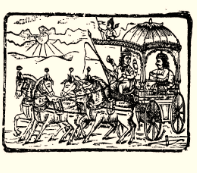
\includegraphics[scale=1.25]{graphics/Capture3.PNG}
\end{minipage}
\vspace*{\fill}
\newpage
%%%%%%%%%%%%%%%%%%%%%%%%%%%%%%%%%%%%%
\hfill
\newpage
%%%%%%%%%%%%%%%%%%%%%%%%%%%%%%%%%%%%%%
\begin{mdframed}
\begin{center}
\large
श्रीमद्वामाचरणभट्टाचार्यविरचितपुस्तकानां प्राप्तिस्थानम्
\end{center}
\vspace{5mm}
\begin{tabular}{lll}
    सिद्धान्तलक्षणजागदीशीविवृतिः&&\\
तर्कसंग्रहदीपिकाविवृतिर्न्यायबोधिन्याष्टिप्पणी च &$\ldots$ &॥।)\\
व्याप्तिपञ्चकमाथुराविवृतिर्जागदीशीविवृतिश्च, &$\ldots$& १  )
\end{tabular}
\begin{flushright}
\large
पता - मास्टर खेलाड़ीलाल एण्ड सन्स्, \\
 कचौड़ीगली, बनारस सिटी~।~
\end{flushright}
 \hrule
\begin{center}
{\large श्रीकृष्णवल्लभाचार्य्यस्वामिनारायणविरचितपुस्तकानां     \\
. प्राप्तिस्थानम्  }\\
तर्कसंग्रहदीपिकाकिरणावली, न्यायबोधिनीपदकृतटिप्पणी च,
\end{center}
\begin{flushright}
\large
 प० 'छन्नूलाल ज्ञानचन्द पाठक,\\
कचौड़ीगली, बनारस~।
\end{flushright}
\begin{center}
श्रीस्वामिनारायणवेदान्तसारः \textemdash\  सांख्यकारिकाभाष्यम्,\\
उपर्युक्तव्याप्तिपञ्चकं च~।   
\end{center}
\begin{flushright}
{\large
  पता\textendash पं० श्रीकृष्णवल्लभाचार्यः, \\
 श्रीस्वामिनारायणमन्दिरम्} \\
अंतपुर, काठिआवाड़~।\\
अथवा \textemdash\;\;\;\;\;\;\;\;\;\;\;\;\;\;\\
{\large बी. जी. ब्रदर्स. चौक.बनारस~।}\\
अथवा\textemdash\;\;\;\;\;\;\;\;\;\;\;\;\;\;\;\\
{\large  नागेश्वरमठ, पटनी टोला, बनारस~।} 
\end{flushright}
\hrule
\begin{center}
श्रीमज्जानकीनाथभट्टाचार्य्यविरचिताऽभिनवव्याख्यया समलङ्कृतं    
\end{center}

किरातार्ज्जुनीयम्\textemdash\ 
\begin{flushright}
{\large पता\textendash मास्टर खेलाड़ीलाल एन्ड सन्स, \\
 कचौड़ीगली, बनारसा~।} \\
 अथवा\textemdash\;\;\;\;\;\;\;\;\;\;\;\;\;\;\;\\
 {\large श्रीमधुसूदनभट्टाचार्य्य, श्रीभूदेव चतुष्पाठी, \\
 मुहल्ला-मानसरोवर, काशी~।~ }
\end{flushright}
\end{mdframed}
 \end{document}